\documentclass[12pt,a4paper]{jarticle}
%%% LaTexパッケージのインクルード %%%
\usepackage{graphicx}
\usepackage{wrapfig}
\usepackage{lscape}
\usepackage{amssymb}
\usepackage{amsmath}
\usepackage{bm}
\usepackage{setspace}
\usepackage{listings,jlisting}
\usepackage{color}
\usepackage{ascmac}
\usepackage{here}
\usepackage[dvipdfmx]{hyperref}
\usepackage{pxjahyper}
\usepackage{enumitem}
\usepackage{itembkbx}
\usepackage{authblk}
%%% ページレイアウト設定 %%%
\topmargin=-5mm
\oddsidemargin=-5mm
\evensidemargin=-5mm
\textheight=235mm
\textwidth=165mm
%%% コマンド定義 %%%
\newcommand{\underbold}[1]{\underline{\bf #1}}
\newcommand{\redtext}[1]{\textcolor{red}{#1}}
%%% \subsubsubsection等の定義 (ここから) %%%
\setcounter{secnumdepth}{6}
\makeatletter
\newcounter{subsubparagraph}[subparagraph]
\renewcommand\thesubsubparagraph{\thesubparagraph.\@arabic\c@subsubparagraph}
\newcommand\subsubparagraph{\@startsection{subsubparagraph}{6}{\parindent}%
                                       {3.25ex \@plus1ex \@minus .2ex}%
                                       {-1em}%
                              {\normalfont\normalsize\bfseries}}
\newcommand*\l@subsubparagraph{\@dottedtocline{6}{10em}{5em}}
\newcommand{\subsubsubsection}{\@startsection{paragraph}{4}{\z@}%
{1.5\baselineskip \@plus.5\dp0 \@minus.2\dp0}%
{.5\baselineskip \@plus2.3\dp0}%
{\reset@font\normalsize\bfseries}
}
\newcommand{\subsubsubsubsection}{\@startsection{subparagraph}{5}{\z@}%
{1.5\baselineskip \@plus.5\dp0 \@minus.2\dp0}%
{.5\baselineskip \@plus2.3\dp0}%
{\reset@font\normalsize\itshape}
}
\newcommand{\subsubsubsubsubsection}{\@startsection{subsubparagraph}{6}{\z@}%
{1.5\baselineskip \@plus.5\dp0 \@minus.2\dp0}%
{.5\baselineskip \@plus2.3\dp0}%
{\reset@font\normalsize\itshape}
}
\setcounter{tocdepth}{6}
%%% \subsubsubsection等の定義 (ここまで) %%%
%%% lstlisting設定 %%%
\lstset{language = C,
numbers = left,
numbersep = 8pt,
breaklines = true,
breakindent = 40pt,
frame = lines,
basicstyle = \ttfamily,
}

\title{FDPS仕様書}
\author{谷川衝}
\author{岩澤全規}
\author{細野七月}
\author{似鳥啓吾}
\author{村主崇行}
\author{行方大輔}
\author{野村昴太郎}
\author{牧野淳一郎}
\affil{理化学研究所 計算科学研究センター 粒子系シミュレータ研究チーム}
\date{}


\begin{document}
\maketitle
\tableofcontents

\newpage

%%%%%%%%%%%%%%%%%%%%%%%%%%%%%%%%%%%%%%%%%%%%%%%%%%%%%
\section{この文書の概要}

This document is the specification of FDPS (Framework for Developing
Particle Simulator), which supports the development of massively
parallel particle simulation codes. This document is written by
Ataru Tanikawa, Masaki Iwasawa, Natsuki Hosono, Keigo Nitadori,
Takayuki Muranushi, and Junichiro Makino at RIKEN Advanced Institute
for Computational Science.
%%この文書は大規模並列粒子シミュレーションの開発を支援するFramework
%%forDeveloping Particle Simulator (FDPS)の仕様書である。この文書は理化
%%学研究所計算科学研究機構粒子系シミュレータ研究チームの谷川衝、岩澤全
%%規、細野七月、似鳥啓吾、村主崇行、牧野淳一郎によって記述された。

This document is structured as follows.
%%この文書は以下のような構成となっている。

In sections~\ref{sec:overview}, \ref{sec:configuration},
and \ref{sec:compile}, we present prerequisites for programing with
FDPS. In section~\ref{sec:overview}, we show the concept of FDPS. In
section~\ref{sec:configuration}, we present the file configuration of
FDPS. In section~\ref{sec:compile}, we describe how to compile
simulation codes with FDPS.
%%節\ref{sec:overview}、\ref{sec:configuration}、\ref{sec:compile}には、
%%FDPSを使ってプログラムを書く際に前提となる情報が記述されている。
%%節\ref{sec:overview}には、FDPSの概要として、FDPSの基本的な考えかたや
%%動作が記述されている。節\ref{sec:configuration}には、FDPSのファイル構
%%成が記述されている。節\ref{sec:compile}には、FDPSのAPIを使用したコー
%%ドをコンパイルする時にどのようなマクロを用いればよいかが記述されてい
%%る。

In sections~\ref{sec:namespace}, \ref{sec:datatype}, \ref{sec:userdefined},
\ref{sec:initfin}, and \ref{sec:module}, we present necessary information
to develop simulation codes with FDPS. In section~\ref{sec:namespace},
we describe the structure of namespaces unused in FDPS. In
section~\ref{sec:datatype}, we described data types defined in
FDPS. In section~\ref{sec:userdefined}, we introduce user-defined
classes and function objects necessary for developing codes with
FDPS. In section~\ref{sec:initfin}, we describe APIs used to
initialize and finalize FDPS. In section~\ref{sec:module}, we present
modules in FDPS and their APIs.
%%節\ref{sec:namespace}、\ref{sec:datatype}、\ref{sec:userdefined}、
%%\ref{sec:initfin}、\ref{sec:module}には、FDPSを使ってプログラムを書く
%%際に必要となる情報が提供されている。節\ref{sec:namespace}には、FDPS内
%%での名前空間の構造についてが記述されている。節\ref{sec:datatype}には、
%%FDPSで独自に定義されているデータ型が記述されている。
%%節\ref{sec:userdefined}には、FDPSのAPIを使用する際にユーザーが定義す
%%る必要があるクラスや関数オブジェクトについて記述されている。
%%節\ref{sec:initfin}には、FDPSを開始するときと終了するときに呼ぶ必要の
%%あるAPIについて記述されている。節\ref{sec:module}には、FDPSにあるモ
%%ジュールとそのAPIについて記述されている。

In
sections~\ref{sec:errormessage}, \ref{sec:knownbug}, \ref{sec:limitation},
and \ref{sec:usersupport}, we present information useful for
troubleshooting.  In section~\ref{sec:errormessage}, we describe error
messages. In section~\ref{sec:knownbug}, we present known bugs. In
section~\ref{sec:limitation}, we describe the limitation of FDPS. In
section~\ref{sec:usersupport}, we present our current system for user
supports.
%%節\ref{sec:errormessage}、\ref{sec:knownbug}、\ref{sec:limitation}、
%%\ref{sec:usersupport}には、FDPSのAPIを使用したコードを記述したがコー
%%ドが思ったように動作しない場合に有用な情報が記載されている。
%%節\ref{sec:errormessage}にはエラーメッセージについてが記述されている。
%%節\ref{sec:knownbug}には、よく知られているバグについて記述されている。
%%節\ref{sec:limitation}には、FDPSの限界について記述されている。
%%節\ref{sec:usersupport}には、ユーザーサポートに関する情報が記述されて
%%いる。

Finally, we describe the license of FDPS in section~\ref{sec:license},
and the change log of this document in section~\ref{sec:changelog}.
%%最後に節\ref{sec:license}にはFDPSのライセンスに関する情報が、
%%節\ref{sec:changelog}にはこの文書の変更履歴が記述されている。


\newpage

%%%%%%%%%%%%%%%%%%%%%%%%%%%%%%%%%%%%%%%%%%%%%%%%%%%%%
\section{FDPS概要}
\label{sec:overview}

この節ではFDPSの概要を記述する。FDPSの開発目的、FDPSの基本的な考えかた、
FDPSを使用して作成したコードの動作について概説する。

%%%%%%%%%%%%%%%%%%%%%%%%%%%%%%%%%%%%%%%%%%%%%%%%%%%%%%%%%%%%%%%%%%%%%%
\subsection{開発目的}

粒子シミュレーションは、重力$N$体シミュレーション、SPHシミュレーション、
渦糸法、MPS法、分子動力学シミュレーションなど理学工学の様々な分野で使
用されている。より大きい空間スケール、より高い空間分解能(または質量分
解能)、より長い時間スケールの物理現象を追跡するために、高性能な粒子シ
ミュレーションコードへの要請はますます強くなっている。

高性能な粒子シミュレーションコードを組むためには、シミュレーションコー
ドの大規模並列化を避けることはできない。粒子シミュレーションコードの大
規模並列化をする際には、ロードバランスのため動的領域分割、領域分割に合
わせた粒子交換、ノード間通信の削減と最適化、キャッシュ利用効率の向上、
SIMDユニット利用効率の向上、アクセラレータへの対応など、数多くの困難な
処理を行う必要がある。現在、研究グループは個別にこれらの処理へ対応して
いる。

しかし、上記の処理は粒子シミュレーション共通のものである。FDPSの開発目
的は、これらの処理を高速に行うライブラリを提供し、大規模並列化への対応
に追われていた研究者の負担を軽くすることである。FDPSを使うことで、研究
者がよりクリエイティブな仕事に専念できるようになれば、幸いである。

%%%%%%%%%%%%%%%%%%%%%%%%%%%%%%%%%%%%%%%%%%%%%%%%%%%%%%%%%%%%%%%%%%%%%%
\subsection{基本的な考えかた}

ここではFDPSの基本的な考えかたについて記述する。

%%%%%%%%%%%%%%%%%%%%%%%%%%%%%%%%%%%%%%%%%%%%%%%%%%%%
\subsubsection{大規模並列粒子シミュレーションの手順}
\label{sec:overview_concept_abstraktion}

まずFDPSにおいて、大規模並列粒子シミュレーションがどのような手順で行わ
れることを想定しているかを記述する。粒子シミュレーションは、以下のよう
な微分方程式を時間発展させるものである。
\begin{align}
    \frac{d\bm{u}_i}{dt} = \sum_j f(\bm{u}_i,\bm{u}_j) + \sum_s
    g(\bm{u}_i,\bm{v}_s) \label{eq:GoverningEquation}
\end{align}
ここで$\bm{u}_i$は粒子$i$の物理量ベクトルであり、この物理量には質量、
位置、速度など粒子が持つあらゆる物理量が含まれる。関数$f$は粒子$j$から
粒子$i$への作用を規定する。以後、作用を受ける粒子を$i$粒子、作用を与え
る粒子を$j$粒子と呼ぶことにする。$\bm{v}_s$は$i$粒子から十分遠方にある
粒子を1つの粒子としてまとめた粒子(以後、この粒子を超粒子と呼ぶ)の物理
量ベクトルである。関数$g$は超粒子から$i$粒子への作用を規定する。式
(\ref{eq:GoverningEquation})の第2項は、重力やクーロン力など無限遠まで
到達する長距離力の場合はゼロではない。しかし流体の圧力のような短距離力
はゼロである。

大規模並列化された粒子シミュレーションコードは以下の手順で式
(\ref{eq:GoverningEquation})を時間発展させる。ここではデータの入出力や
初期化は省略している。
\begin{enumerate}
\item 以下の2段階の手順でどのプロセスがどの粒子の式
  (\ref{eq:GoverningEquation})を時間発展させるか決める。
  \label{item:LoadBalance}
  \begin{enumerate}
  \item プロセスの間でロードバランスを取れるように、シミュレーションで
    扱っている空間の領域を分割し、各プロセスの担当領域を決める(領域分
    割)。
  \item 各プロセスが、自分の担当する領域に存在する全粒子の物理量ベクト
    ル$\bm{u}_i$を持つように、他のプロセスと物理量ベクトル$\bm{u}_i$を
    交換する(粒子交換)。
  \end{enumerate}

\item 各プロセスは、自分の担当する全粒子の式
  (\ref{eq:GoverningEquation})の右辺を計算するのに必要な$j$粒子の物理
  量ベクトル$\bm{u}_j$と超粒子の物理量ベクトル$\bm{v}_s$を他のプロセス
  と通信することで集めて、$j$粒子のリストと超粒子のリスト(まとめて相互
  作用リストと呼ぶ)を作る(相互作用リストの作成)。
  \label{item:MakeInteractionList}

\item 各プロセスは自分の担当する全粒子に対して、式
  (\ref{eq:GoverningEquation})の右辺を計算し、$d\bm{u}_i/dt$を求める
  (相互作用の計算)。\label{item:CalcInteraction}

\item 各プロセスは、自分の担当する全粒子の物理量ベクトル$\bm{u}_i$とそ
  の時間導関数$d\bm{u}_i/dt$を使って、全粒子の時間積分を実行し、次の時
  刻の物理量ベクトル$\bm{u}_i$を求める(時間積分)。
  \label{item:IntegrateTime}

\item 手順\ref{item:LoadBalance}に戻る。        
\end{enumerate}

%%    ただし、あらゆる相互作用のタイプに対応するには以下5種類の$j$粒子
%%    と超粒子の集め方が必要。\label{item:MakeInteractionList}    
%%    \begin{itemize}
%%        \item 長距離力モード:$i$粒子に対して、近い粒子は$j$粒子として、
%%        遠方の複数の粒子はまとめて超粒子として集めるモード(使用例:開
%%        放条件下の重力やクーロン力)
%%        \item 長距離力モードカットオフ付き:長距離力モードとほぼ同じだ
%%        が、ある距離より遠い粒子は集めないモード(使用例:周期境界条件
%%        下の重力やクーロン力)
%%        \item 短距離力収集モード:$i$粒子自身の持つサーチ半径の内側に
%%        ある粒子のみ$j$粒子として集めるモード(使用例:SPH法における密
%%        度の計算)
%%        \item 短距離力散乱モード:$i$粒子をサーチ半径の内側に含む粒子
%%        を$j$粒子として集めるモード(使用例:Lennard-Jones力)
%%        \item 短距離力対称モード:短距離力収集モードで集める粒子と短距
%%        離力散乱モードで集める粒子の和集合を$j$粒子として集めるモード
%%        (使用例:SPH法における圧力勾配の計算)    
%%    \end{itemize}

%%%%%%%%%%%%%%%%%%%%%%%%%%%%%%%%%%%%%%%%%%%%%%%%%%%%
\subsubsection{ユーザーとFDPSの役割分担}

FDPSは、プロセス間の通信が発生する処理はFDPSが担当し、プロセス間の通信
の発生しない処理はユーザーが担当するという役割分担を基本としている。従っ
て、前節に挙げた、領域分割・粒子交換(項目\ref{item:LoadBalance})・相互
作用リストの作成(項目\ref{item:MakeInteractionList})をFDPSが、相互作用
の計算(項目\ref{item:CalcInteraction})・時間積分(項目
\ref{item:IntegrateTime})をユーザーが担当することになる。ユーザーは
FDPSのAPIを呼び出すだけで、大規模並列化に関わる煩雑な処理を避けつつ、
高性能な任意の相互作用の粒子シミュレーションコードを手に入れることがで
きる。

%%%%%%%%%%%%%%%%%%%%%%%%%%%%%%%%%%%%%%%%%%%%%%%%%%%%
\subsubsection{ユーザーのやること}

ユーザーがFDPSを使って粒子シミュレーションコードを作成するときにやるこ
とは以下の項目である。
\begin{itemize}

%%\item 座標系の選択(節\ref{sec:compile_coordinate})。2次元または3次元
%%  直角座標系の選択が可能。

%%\item 境界条件の選択(節\ref{sec:datatype_enum_boundarycondition})。開
%%  放境界条件、x, y, z軸方向どれかまたはすべての周期境界条件の選択が可
%%  能。
    
\item 粒子の定義(節\ref{sec:userdefined})。粒子の持つ物理量(式
  (\ref{eq:GoverningEquation})で言えば$\bm{u}_i$)の指定。例えば質量、
  位置、速度、加速度、元素組成、粒子サイズ、など。

\item 相互作用の定義(節\ref{sec:userdefined})。粒子間の相互作用(式
  (\ref{eq:GoverningEquation})で言えばで関数$f$, $g$)を指定。例えば、
  重力、クーロン力、圧力、など。

\item FDPSのAPIの呼出(節\ref{sec:initfin}, \ref{sec:module})

\end{itemize}

%%%%%%%%%%%%%%%%%%%%%%%%%%%%%%%%%%%%%%%%%%%%%%%%%%%%
\subsubsection{補足}

式(\ref{eq:GoverningEquation})の右辺は2粒子間相互作用の重ね合わせであ
る。従って、FDPSのAPIを呼ぶだけでは、3つ以上の粒子の間の相互作用の計算
を行うことはできない。しかし、FDPSはネイバーリストを返すAPIを用意して
いる。ネイバーリストを用いれば、ユーザーはプロセス間の通信の処理をする
ことなく、このような相互作用の計算をできる。

節\ref{sec:overview_concept_abstraktion}で示した手順は、全粒子が同じ時
間刻みを持っている。そのため、FDPSのAPIを呼び出すだけでは、独立時間刻
みで時間積分を効率的に行うことができない。しかし、上と同じくネイバーリ
ストを返すAPIがあるため、Particle Particle Particle Tree法を用いて独立
時間刻みを実装することは可能であろう。

%%マルチプロセス, マルチスレッド, SIMD演算を用いて, 並列に処理される.
%%FDPSはC++言語にて記述される.

%%%%%%%%%%%%%%%%%%%%%%%%%%%%%%%%%%%%%%%%%%%%%%%%%%%%%%%%%%%%%%%%%%%%%%
\subsection{コードの動作}
\label{sec:overview_action}

ここではFDPSを使用して作成したコードの動作の概略を記述する。このコード
には、4つのモジュールがあることになる。3つはFDPSのモジュールで、1つ
はユーザー定義のモジュールである。まとめると以下のようになる。
\begin{itemize}
\item 領域クラス:全プロセスが担当する領域の情報と、領域分割を行うAPI
  を持つ
\item 粒子群クラス:全粒子の情報と、プロセスの間での粒子交換を行うAPI
  を持つ
\item 相互作用ツリークラス:粒子分布から作られたツリー構造と、相互作用
  リストを作成するAPIを持つ
\item ユーザー定義クラス:ある1粒子を定義するクラス、粒子間の相互作用
  を定義する関数オブジェクトを持つ
\end{itemize}

これら4つのモジュールの間で情報がやり取りされる。これは図
\ref{fig:brief_interface}で概観できる。図\ref{fig:brief_interface}に示
された情報のやりとりは、節\ref{sec:overview_concept_abstraktion}に記述
された手順\ref{item:LoadBalance}から\ref{item:CalcInteraction}と、これ
らの手順以前に行われる手順(手順0とする)に対応する。
以下はこれらの手順の詳細な記述である。
\begin{enumerate}
\item[0.] ユーザー定義クラスのうち1粒子を定義するクラスが粒子群クラス
  へ、粒子間の相互作用を定義する関数オブジェクトが相互作用ツリークラス
  へ渡される。これはクラスの継承ではなく、粒子を定義するクラスは粒子群
  クラスのテンプレート引数として、粒子間の相互作用を定義する関数オブジェ
  クトは相互作用ツリークラスのAPIの引数として渡される
\item[\ref{item:LoadBalance}.] 以下の2段階でロードバランスを取る
  \begin{enumerate}
  \item 領域クラスが持つ領域分割のAPIが呼ばれる。このとき粒子情報が粒
    子群クラスから領域クラスへ渡される (赤字と赤矢印)
  \item 粒子群クラスが持つ粒子交換のAPIが呼ばれる。このとき領域情報が
    領域クラスから粒子群クラスへ渡される (青字と青矢印)
  \end{enumerate}
\item[\ref{item:MakeInteractionList}.] 相互作用ツリークラスが持つ相互
  作用リストを作成するAPIが呼ばれる。このとき領域情報が領域クラスから
  相互作用ツリークラスへ、粒子情報が粒子群クラスから相互作用ツリークラ
  スへ渡される (緑字と緑矢印)
\item[\ref{item:CalcInteraction}.] 相互作用ツリーククラスが持つ相互作
  用を定義した関数オブジェクトを呼び出すAPIが呼ばれる。相互作用計算が
  実行され、相互作用計算の結果が相互作用ツリークラスから粒子群クラスへ
  渡される (灰色の字と灰色矢印)
\end{enumerate}

%% ルートドメイン
%% ドメイン
%% リアル粒子
%% フル粒子
%% イメージ粒子
%% セル
%% リーフ

\begin{figure}[h]
  \begin{center}
    %    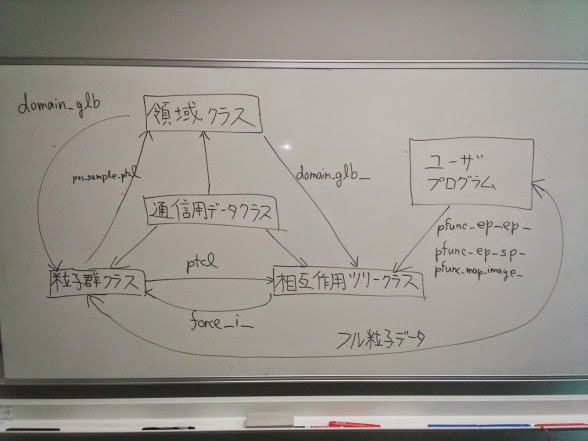
\includegraphics[width=10cm,bb=0 0 600 500]{fig/brief_interface.jpg}
    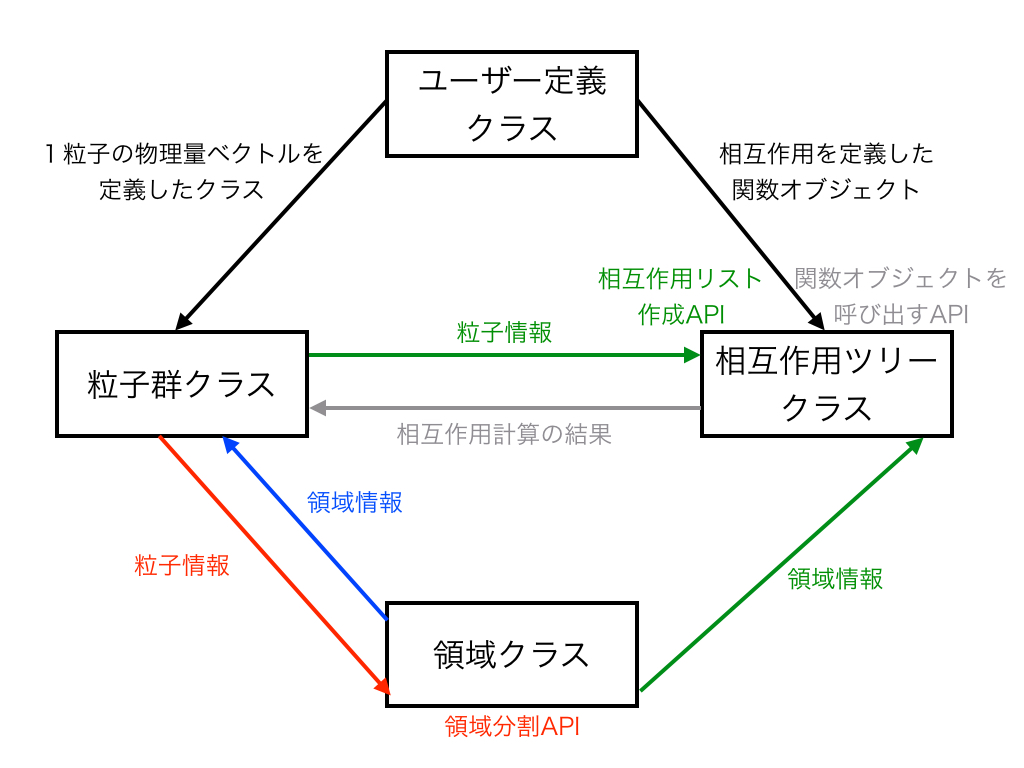
\includegraphics[width=10cm,bb=0 0 700 700]{fig/illustration/illustration.001.jpg}
  \end{center}
  \caption{モジュールインターフェースと情報の流れの模式図。}
  \label{fig:brief_interface}
\end{figure}


\newpage

%%%%%%%%%%%%%%%%%%%%%%%%%%%%%%%%%%%%%%%%%%%%%%%%%%%%%
\section{ファイル構成}
\label{sec:configuration}

\subsection{概要}

ここではFDPSのファイル構成について記述する。ドキュメント、ソースファイ
ル、テストコード、サンプルコードの順に記述する。

\subsection{ドキュメント}

ドキュメント関係のファイルはディレクトリdocの下にある。チュートリアル
がdoc\_tutorial.pdfであり、仕様書がdoc\_specs.pdfである。

\subsection{ソースファイル}

ソースファイルはディレクトリsrcの下にある。標準機能関係のソースファイ
ルはsrcの直下にある。ディレクトリsrcの直下にあるヘッダファイル
particle\_simulator.hppをソースファイルにインクルードすれば、FDPSの標準
機能を使用できるようになる。

\subsubsection{拡張機能}

拡張機能関係のソースファイルはディレクトリsrcの直下のディレクトリにそ
れぞれ入っている。拡張機能にはParticle Mesh、x86版Phantom-GRAPEがある。

\subsubsubsection{Particle Mesh}

Particle Meshのソースファイルはディレクトリsrc/particle\_meshの下にあ
る。ここでMakefileを編集して、makeを実行すると、ヘッダファイル
particle\_mesh\_class.hppとライブラリlibpm.aができる。このヘッダファイル
をインクルードし、このライブラリをリンクづけすれば、Particle Meshの機
能を使用できるようになる。

\subsubsubsection{x86版Phantom-GRAPE}

x86版Phantom-GRAPEのソースファイルはディレクトリ
src/phantom\_GRAPE\_x86の下にある。この下には低精度N体シミュレーション
用、低精度カットオフ付き相互作用計算用
、高精度N体シミュレーション用(ディレクトリ
G6/libavx)がある。それぞれについて述べる。

\subsubsubsubsection{低精度N体シミュレーション用}

これはディレクトリsrc/phantom\_GRAPE\_x86/G5/newton/libpg5にある。この
ディレクトリ内のMakefileを編集して、makeを実行すると、ライブラリ
libpg5.aができる。このディレクトリ内のヘッダファイルgp5util.hをインク
ルードし、ライブラリlibpg5.aをリンクすると、このPhantom-GRAPEが使用可
能になる。

\subsubsubsubsection{低精度カットオフ付き相互作用計算用}

これはディレクトリsrc/phantom\_GRAPE\_x86/G5/table/にある。このディレ
クトリ内のMakefileを編集して、makeを実行すると、ライブラリlibpg5.aがで
きる。このディレクトリ内のヘッダファイルgp5util.hをインクルードし、ラ
イブラリlibpg5.aをリンクすると、このPhantom-GRAPEが使用可能になる。

\subsubsubsubsection{高精度N体シミュレーション用}

これはディレクトリsrc/phantom\_GRAPE\_x86/G6/libavx/にある。このディレ
クトリ内のMakefileを編集して、makeを実行すると、ライブラリlibg6avx.aが
できる。このディレクトリ内のヘッダファイルgp6util.hをインクルードし、
ライブラリlibg6avx.aをリンクすると、このPhantom-GRAPEが使用可能になる。

\subsection{テストコード}

テストコードはディレクトリtestsの下にある。ディレクトリtestsにカレント
ディレクトリを移し、make checkを実行するとテストスィートが動作する。

\subsection{サンプルコード}

サンプルコードはディレクトリsampleの下にある。サンプルコードは2つ用意
されており、重力N体シミュレーションとSPHシミュレーションである。

\subsubsection{重力N体シミュレーション}

ディレクトリsample/nbodyの下にソースファイルがある。サンプルコードの実
行方法はチュートリアルを参照のこと。

\subsubsection{SPHシミュレーション}

ディレクトリsample/sphの下にソースファイルがある。サンプルコードの実
行方法はチュートリアルを参照のこと。


\newpage

%%%%%%%%%%%%%%%%%%%%%%%%%%%%%%%%%%%%%%%%%%%%%%%%%%%%%
\section{コンパイル時のマクロによる選択}
\label{sec:compile}

\subsection{概要}

FDPSでは、座標系、並列処理の有無、浮動小数点数型の精度、ツリーの最大の
深さ、粒子ソートのアルゴリズム等を選択できる。この選択はコンパイル時の
マクロの定義によってなされる。以下、それぞれの選択の方法を記述する。

\subsection{座標系}
\label{sec:compile_coordinate}

\subsubsection{概要}

座標系は直角座標系3次元と直角座標系2次元の選択ができる。以下、それら
の選択方法について述べる。

\subsubsection{直角座標系3次元}

デフォルトは直角座標系3次元である。なにも行わなくても直角座標系3次元
となる。

\subsubsection{直角座標系2次元}

コンパイル時にPARTICLE\_SIMULATOR\_TWO\_DIMENSIONをマクロ定義すると直
交座標系2次元となる。

\subsection{並列処理}

\subsubsection{概要}

並列処理に関しては、OpenMPの使用/不使用、MPIの使用/不使用を選択でき
る。以下、選択の仕方について記述する。

\subsubsection{OpenMPの使用}

デフォルトはOpenMP不使用である。使用する場合は、
\\ PARTICLE\_SIMULATOR\_THREAD\_PARALLELをマクロ定義すればよい。GCCコ
ンパイラの場合はコンパイラオプションに-fopenmpをつける必要がある。

\subsubsection{MPIの使用}

デフォルトはMPI不使用である。使用する場合は、
PARTICLE\_SIMULATOR\_THREAD\_PARALLELをマクロ定義すればよい。

\subsection{データ型の精度}
\subsubsection{概要}
FDPS側で用意したMomentクラス(第7.5.2節参照)とSuperParticleJクラス(第7.6.2節参照)のデータ型の精度を選択できる。以下、選択の仕方について記述する。

\subsubsection{既存のSuperParticleJクラスとMomentクラスの精度}
既存のSuperParticleJクラスとMomentクラスのメンバ変数の精度はデフォルトで64ビットである。32ビットにしたい場合、\\
PARTICLE\_SIMULATOR\_SPMOM\_F32 \\
をマクロ定義すればよい。


%\subsubsection{Vector型の範囲チェック}
%\label{sec:compile:vector_invalid_access}

%コンパイル時にPARTICLE\_SIMULATOR\_VECTOR\_RANGE\_CHECKをマクロ定義す
%るとVector型の範囲外の成分にアクセスするとエラーメッセージを出力するこ
%とが出来る。詳しくは節\ref{sec:errormessage:vector_invalid_access}を参
%照。


\subsection{ツリーの最大深さ(レベル)の変更}
\label{sec:compile_tree_level}


ツリー構造は粒子の位置座標のモートンキーを用いて作られているため、ツリー
の最大レベルはモートンキーのビット長に依存する.FDPSでは3次元シミュレー
ションの場合にのみ,適切なマクロを指定することにより、粒子のモートンキー
を64bit(レベル21),96bit(最大レベル31),128bit(最大レベル42)の3つから
選択することができる.特にマクロを指定しなければ,キーの長さは128bitに
なる.キーを96bitにする場合はPARTICLE\_SIMULATOR\_USE\_96BIT\_KEYを,
64bitにする場合はPARTICLE\_SIMULATOR\_USE\_64BIT\_KEYをマクロ定義す
ればよい.

アーキテクチャによっては短いキーとすることで若干の高速化やメモリ節約が
実現できるが、特に64ビットキーでは粒子分布によってはレベルが不足する。

\subsection{粒子のソートの方法の変更}
\label{sec:compile_sort_method}

{\tt TreeForForce}クラスの内部では粒子はモートンキーの順でソートされて
いる.デフォルトではソートアルゴリズムとしてマージソートが使われている
が,PARTICLE\_SIMULATOR\_USE\_RADIX\_SORTをマクロ定義することでソート
アルゴリズムを基数ソートに変更できる.

アーキテクチャによっては基数ソートが若干速いかもしれない。





\newpage

%%%%%%%%%%%%%%%%%%%%%%%%%%%%%%%%%%%%%%%%%%%%%%%%%%%%%
\section{名前空間}
\label{sec:namespace}

%\subsection{概要}
\subsection{Summary}

In this section, we describe the namespaces used in FDPS. All the FDPS
APIs are under namespace \texttt{ParticleSimulator}. In the
following, we show APIs directly under \texttt{ParticleSimulator}, and
namespaces nested under \texttt{ParticleSimulator}.
%%本節では、名前空間の構造について述べる。FDPSはParticleSimulatorという
%%名前空間で囲まれている。以下では、ParticleSimulator直下にある機能と、
%%ParticleSimulatorにネストされている名前空間について述べる。

\subsection{ParticleSimulator}

The standard features of FDPS are in namespace \texttt{ParticleSimulator}.
%FDPSの標準機能すべては名前空間ParticleSimulatorの直下にある。

Namespace \texttt{ParticleSimulator} is abbreviated to \texttt{PS} as follows.
%名前空間ParticleSimulatorは以下のように省略されており、この文書におけ
%るあとの記述でもこの省略形を採用する。
\begin{screen}
\begin{verbatim}
namespace PS = ParticleSimulator;
\end{verbatim}
\end{screen}
In this document, we use this abbreviation.

Extended features of FDPS are grouped under nested namespaces.
Currently, \texttt{ParticleMesh} features is under nested namespace
\texttt{ParticleMesh}.  In the following, we describe this namespace
containing the extended features.
%名前空間ParticleSimulatorの下にはいくつかの名前空間が拡張機能毎にネストされている。拡
%張機能にはParticleMeshがある。以下では拡張機能の名前空間について記述す
%る。

\subsubsection{ParticleMesh}

The features of Particle Mesh are under namespace \texttt{PartcielMesh}.
This namespace is abbreviated to \texttt{PM} as follows.
%Particle Meshの機能は名前空間PartcielMeshに囲まれており、名前空間
%ParticleMeshは名前空間ParticleSimulatorの直下にネストされている。また、
%ParticleMeshはPMと省略されている。これらをまとめると以下のようになって
%いる。
\begin{screen}
\begin{verbatim}
ParticleSimulator {
    ParticleMesh {
    }
    namespace PM = ParticleMesh;
}
\end{verbatim}
\end{screen}

In this document, we use this abbreviation.
%以後、この文書では省略形のPMを用いて記述する。

\newpage

%%%%%%%%%%%%%%%%%%%%%%%%%%%%%%%%%%%%%%%%%%%%%%%%%%%%%
\section{データ型}
\label{sec:datatype}

\subsection{概要}

FDPSでは独自の整数型、実数型、ベクトル型、対称行列型、PS::SEARCH\_MODE
型、列挙型が定義されている。整数型、実数型、ベクトル型、対称行列型に関
しては必ずしもここに挙げるものを用いる必要はないが、これらを用いること
を推奨する。PS::SEARCH\_MODE型、列挙型は必ず用いる必要がある。以下、整
数型、実数型、ベクトル型、対称行列型、PS::SEARCH\_MODE型、列挙型の順に
記述する。

\subsection{整数型}

%\subsubsection{概要}
\subsubsection{Overview}

The integer types are PS::S32, PS::S64, PS::U32, and PS::U64. We
describe these data types in this section.

%整数型にはPS::S32, PS::S64, PS::U32, PS::U64がある。以下、順にこれらを
%記述する。

\subsubsection{PS::S32}

PS::S32, which is 32-bit signed integer, is defined as follows.
%PS::S32は以下のように定義されている。すなわち32bitの符号付き整数である。
\begin{lstlisting}[caption=S32]
namespace ParticleSimulator {
    typedef int S32;
}
\end{lstlisting}

%Safe performance is ensured, only when users adopt GCC and K compilers.
%ただし、GCCコンパイラとKコンパイラでのみ32bitであることが保証されている。

\subsubsection{PS::S64}

PS::S64, which is 64-bit signed integer, is defined as follows.
%PS::S64は以下のように定義されている。すなわち64bitの符号付き整数である。
\begin{lstlisting}[caption=S64]
namespace ParticleSimulator {
    typedef long long int S64;
}
\end{lstlisting}

%Safe performance is ensured, only when users adopt GCC and K compilers.
%ただし、GCCコンパイラとKコンパイラでのみ64bitであることが保証されている。

\subsubsection{PS::U32}

PS::U32, which is 32-bit unsigned integer, is defined as follows.
%PS::U32は以下のように定義されている。すなわち32bitの符号なし整数である。
\begin{lstlisting}[caption=U32]
namespace ParticleSimulator {
    typedef unsigned int U32;
}
\end{lstlisting}

%Safe performance is ensured, only when users adopt GCC and K compilers.
%ただし、GCCコンパイラとKコンパイラでのみ32bitであることが保証されている。

\subsubsection{PS::U64}

PS::U64, which is 64-bit unsigned integer, is defined as follows.
%PS::U64は以下のように定義されている。すなわち64bitの符号なし整数である。
\begin{lstlisting}[caption=U64]
namespace ParticleSimulator {
    typedef unsigned long long int U64;
}
\end{lstlisting}

%Safe performance is ensured, only when users adopt GCC and K compilers.
%ただし、GCCコンパイラとKコンパイラでのみ64bitであることが保証されている。



\subsection{実数型}

\subsubsection{Abstract}

The floating point types are PS::F32 and PS::F64. We described
these data types in this section.
%実数型にはPS::F32, PS::F64がある。以下、順にこれらを記述する。

\subsubsection{PS::F32}

PS::F32, which is 32-bit floating point number, is defined as follows.
%PS::F32は以下のように定義されている。すなわち32bitの浮動小数点数である。
\begin{lstlisting}[caption=F32]
namespace ParticleSimulator {
    typedef float F32;
}
\end{lstlisting}

\subsubsection{PS::F64}

PS::F64, which is 64-bit floating point number, is defined as follows.
%PS::F64は以下のように定義されている。すなわち64bitの浮動小数点数である。
\begin{lstlisting}[caption=F64]
namespace ParticleSimulator {
    typedef double F64;
}
\end{lstlisting}


\subsection{ベクトル型}

\subsubsection{Abstract}

The vector types are \texttt{PS::Vector2} (2D vector) and
\texttt{PS::Vector3} (3D vector). We describe these vector types first.
These are template classes, which can take basic datatypes
as \texttt{F32} or \texttt{F64} as template arguments. We then present
wrappers for these vector types.

%%ベクトル型には2次元ベクトル型PS::Vector2と3次元ベクトル型PS::Vector3
%%がある。まずこれら2つを記述する。最後にこれらベクトル型のラッパーに
%%ついて記述する。

\subsubsection{PS::Vector2}

PS::Vector2はx, yの2要素を持つ。これらに対する様々なAPIや演算子を定義
した。それらの宣言を以下に記述する。この節ではこれらについて詳しく記述
する。
\begin{lstlisting}[caption=Vector2]
namespace ParticleSimulator{
    template <typename T>
    class Vector2{
    public:
        //メンバ変数2要素
        T x, y;

        //コンストラクタ
        Vector2();
        Vector2(const T _x, const T _y) : x(_x), y(_y) {}
        Vector2(const T s) : x(s), y(s) {}
        Vector2(const Vector2 & src) : x(src.x), y(src.y) {}

        //代入演算子
        const Vector2 & operator = (const Vector2 & rhs);

        //[]演算子
        const T & opertor[](const int i);
        T & operator[](const int i);

        //加減算
        Vector2 operator + (const Vector2 & rhs) const;
        const Vector2 & operator += (const Vector2 & rhs);
        Vector2 operator - (const Vector2 & rhs) const;
        const Vector2 & operator -= (const Vector2 & rhs);

        //ベクトルスカラ積
        Vector2 operator * (const T s) const;
        const Vector2 & operator *= (const T s);
        friend Vector2 operator * (const T s,
                                   const Vector2 & v);
        Vector2 operator / (const T s) const;
        const Vector2 & operator /= (const T s);

        //内積
        T operator * (const Vector2 & rhs) const;

        //外積(返り値はスカラ!!)
        T operator ^ (const Vector2 & rhs) const;

        //Vector2<U>への型変換
        template <typename U>
        operator Vector2<U> () const;
    };
}
namespace PS = ParticleSimulator;
\end{lstlisting}

\subsubsubsection{コンストラクタ}

\begin{screen}
\begin{verbatim}
template<typename T>
PS::Vector2<T>::Vector2()
\end{verbatim}
\end{screen}

\begin{itemize}

\item{{\bf 引数}}

なし。

\item{{\bf 機能}}

デフォルトコンストラクタ。メンバx,yは0で初期化される。

\end{itemize}

%%%%%%%%%%%%%%%%%%%%%%%%%%%%%
\begin{screen}
\begin{verbatim}
template<typename T>
PS::Vector2<T>::Vector2(const T _x, const T _y)
\end{verbatim}
\end{screen}

\begin{itemize}

\item{{\bf 引数}}

{\_x}: 入力。{const T}型。

{\_y}: 入力。{const T}型。

\item{{\bf 機能}}

メンバ{x}、{y}をそれぞれ{\_x}、{\_y}で初期化する。

\end{itemize}

%%%%%%%%%%%%%%%%%%%%%%%%%%%%%
\begin{screen}
\begin{verbatim}
template<typename T>
PS::Vector2<T>::Vector2(const T s);
\end{verbatim}
\end{screen}

\begin{itemize}

\item{{\bf 引数}}

{s}: 入力。{const T}型。

\item{{\bf 機能}}

メンバ{x}、{y}を両方とも{s}の値で初期化する。

\end{itemize}

%%%%%%%%%%%%%%%%%%%%%%%%%%%%%
\subsubsubsection{コピーコンストラクタ}

\begin{screen}
\begin{verbatim}
template<typename T>
PS::Vector2<T>::Vector2(const PS::Vector2<T> & src)
\end{verbatim}
\end{screen}

\begin{itemize}

\item{{\bf 引数}}

{src}: 入力。{const PS::Vector2$<$T$>$ \&}型。

\item{{\bf 機能}}

コピーコンストラクタ。{src}で初期化する。

\end{itemize}

%%%%%%%%%%%%%%%%%%%%%%%%%%%%%
\subsubsubsection{メンバ変数}

\begin{screen}
\begin{verbatim}
template<typename T>
T PS::Vector2<T>::x;

template<typename T>
T PS::Vector2<T>::y;
\end{verbatim}
\end{screen}

\begin{itemize}
  
\item{{\bf 機能}}
  
  メンバ{x}、{y}を直接操作出来る。
  
\end{itemize}

%%%%%%%%%%%%%%%%%%%%%%%%%%%%%
\subsubsubsection{代入演算子}

\begin{screen}
\begin{verbatim}
template<typename T>
const PS::Vector2<T> & PS::Vector2<T>::operator = 
                       (const PS::Vector2<T> & rhs);
\end{verbatim}
\end{screen}

\begin{itemize}

\item{{\bf 引数}}

{rhs}: 入力。{const PS::Vector2$<$T$>$ \&}型。

\item{{\bf 返り値}}

{const PS::Vector2$<$T$>$ \&}型。{rhs}のx,yの値を自身のメンバx,yに
代入し自身の参照を返す。代入演算子。

\end{itemize}

\subsubsubsection{[]演算子}

\begin{screen}
\begin{verbatim}
template<typename T>
const T & PS::Vector2<T>::operator[]
                       (const int i);
\end{verbatim}
\end{screen}

\begin{itemize}

\item{{\bf 引数}}

  {i}: 入力。{const int}型。

\item{{\bf 返り値}}

  {const $<$T$>$ \&}型。ベクトルのi成分を返す。
  
\item{{\bf 備考}}

  直接メンバ変数を指定する場合に比べ、処理が遅くなることがある。

\end{itemize}

\begin{screen}
\begin{verbatim}
template<typename T>
T & PS::Vector2<T>::operator[]
                       (const int i);
\end{verbatim}
\end{screen}

\begin{itemize}

\item{{\bf 引数}}

{i}: 入力。{const int}型。

\item{{\bf 返り値}}

{$<$T$>$ \&}型。ベクトルのi成分を返す。

\item{{\bf 備考}}

  直接メンバ変数を指定する場合に比べ、処理が遅くなることがある。

\end{itemize}

\subsubsubsection{加減算}

\begin{screen}
\begin{verbatim}
template<typename T>
PS::Vector2<T> PS::Vector2<T>::operator + 
               (const PS::Vector2<T> & rhs) const;
\end{verbatim}
\end{screen}

\begin{itemize}

\item{{\bf 引数}}

{rhs}: 入力。{const PS::Vector2$<$T$>$ \&}型。

\item{{\bf 返り値}}

{PS::Vector2$<$T$>$}型。{rhs}のx,yの値と自身のメンバx,yの値の和を
取った値を返す。

\end{itemize}

\begin{screen}
\begin{verbatim}
template<typename T>
const PS::Vector2<T> & PS::Vector2<T>::operator += 
                       (const PS::Vector2<T> & rhs);
\end{verbatim}
\end{screen}

\begin{itemize}

\item{{\bf 引数}}

{rhs}: 入力。{const PS::Vector2$<$T$>$ \&}型。

\item{{\bf 返り値}}

{const PS::Vector2$<$T$>$ \&}型。{rhs}のx,yの値を自身のメンバx,yに足し、自
身を返す。

\end{itemize}

\begin{screen}
\begin{verbatim}
template<typename T>
PS::Vector2<T> PS::Vector2<T>::operator - 
               (const PS::Vector2<T> & rhs) const;
\end{verbatim}
\end{screen}

\begin{itemize}

\item{{\bf 引数}}

{rhs}: 入力。{const PS::Vector2$<$T$>$ \&}型。

\item{{\bf 返り値}}

{PS::Vector2$<$T$>$}型。{rhs}のx,yの値と自身のメンバx,yの値の差を
取った値を返す。

\end{itemize}

\begin{screen}
\begin{verbatim}
template<typename T>
const PS::Vector2<T> & PS::Vector2<T>::operator -= 
                       (const PS::Vector2<T> & rhs);
\end{verbatim}
\end{screen}

\begin{itemize}

\item{{\bf 引数}}

{rhs}: 入力。{const PS::Vector2$<$T$>$ \&}型。

\item{{\bf 返り値}}

{const PS::Vector2$<$T$>$ \&}型。自身のメンバx,yから{rhs}のx,yを引
き自身を返す。

\end{itemize}

\subsubsubsection{ベクトルスカラ積}

\begin{screen}
\begin{verbatim}
template<typename T>
PS::Vector2<T> PS::Vector2<T>::operator * (const T s) const;
\end{verbatim}
\end{screen}

\begin{itemize}

\item{{\bf 引数}}

{s}: 入力。{const T}型。

\item{{\bf 返り値}}

{PS::Vector2$<$T$>$}型。自身のメンバx,yそれぞれに{s}をかけた値を返
す。

\end{itemize}

\begin{screen}
\begin{verbatim}
template<typename T>
const PS::Vector2<T> & PS::Vector2<T>::operator *= (const T s);
\end{verbatim}
\end{screen}

\begin{itemize}

\item{{\bf 引数}}

{rhs}: 入力。{const T}型。

\item{{\bf 返り値}}

{const PS::Vector2$<$T$>$ \&}型。自身のメンバx,yそれぞれに{s}をかけ
自身を返す。

\end{itemize}

\begin{screen}
\begin{verbatim}
template<typename T>
PS::Vector2<T> PS::Vector2<T>::operator / (const T s) const;
\end{verbatim}
\end{screen}

\begin{itemize}

\item{{\bf 引数}}

{s}: 入力。{const T}型。

\item{{\bf 返り値}}

{PS::Vector2$<$T$>$}型。自身のメンバx,yそれぞれを{s}で割った値を返
す。

\end{itemize}

\begin{screen}
\begin{verbatim}
template<typename T>
const PS::Vector2<T> & PS::Vector2<T>::operator /= (const T s);
\end{verbatim}
\end{screen}

\begin{itemize}

\item{{\bf 引数}}

{rhs}: 入力。{const T}型。

\item{{\bf 返り値}}

{const PS::Vector2$<$T$>$ \&}型。自身のメンバx,yそれぞれを{s}で割り
自身を返す。

\end{itemize}

\subsubsubsection{内積、外積}

\begin{screen}
\begin{verbatim}
template<typename T>
T PS::Vector2<T>::operator * (const PS::Vector2<T> & rhs) const;
\end{verbatim}
\end{screen}

\begin{itemize}

\item{{\bf 引数}}

{rhs}: 入力。{const PS::Vector2$<$T$>$ \&}型。

\item{{\bf 返り値}}

{T}型。自身と{rhs}の内積を取った値を返す。

\end{itemize}

\begin{screen}
\begin{verbatim}
template<typename T>
T PS::Vector2<T>::operator ^ (const PS::Vector2<T> & rhs) const;
\end{verbatim}
\end{screen}

\begin{itemize}

\item{{\bf 引数}}

{rhs}: 入力。{const PS::Vector2$<$T$>$ \&}型。

\item{{\bf 返り値}}

{T}型。自身と{rhs}の外積を取った値を返す。

\end{itemize}

\subsubsubsection{{Vector2$<$U$>$}への型変換}

\begin{screen}
\begin{verbatim}
template<typename T>
template <typename U>
PS::Vector2<T>::operator PS::Vector2<U> () const;
\end{verbatim}
\end{screen}

\begin{itemize}

\item{{\bf 引数}}

  なし。

\item{{\bf 返り値}}

  {const PS::Vector2$<$U$>$}型。

\item{{\bf 機能}}

  {const PS::Vector2$<$T$>$}型を{const PS::Vector2$<$U$>$}型にキャ
  ストする。

\end{itemize}




\subsubsection{PS::Vector3}

PS::Vecotr3はx, y, zの3要素を持つ。これらに対する様々なAPIや演算子を定
義した。それらの宣言を以下に記述する。この節ではこれらについて詳しく記
述する。
\begin{lstlisting}[caption=Vector3]
namespace ParticleSimulator{
    template <typename T>
    class Vector3{
    public:
        //メンバ変数は以下の二つのみ。
        T x, y, z;

        //コンストラクタ
        Vector3() : x(T(0)), y(T(0)), z(T(0)) {}
        Vector3(const T _x, const T _y, const T _z) : x(_x), y(_y), z(_z) {}
        Vector3(const T s) : x(s), y(s), z(s) {}
        Vector3(const Vector3 & src) : x(src.x), y(src.y), z(src.z) {}

        //代入演算子
        const Vector3 & operator = (const Vector3 & rhs);

        //[]演算子
        const T & opertor[](const int i);
        T & operator[](const int i);

        //加減算
        Vector3 operator + (const Vector3 & rhs) const;
        const Vector3 & operator += (const Vector3 & rhs);
        Vector3 operator - (const Vector3 & rhs) const;
        const Vector3 & operator -= (const Vector3 & rhs);

        //ベクトルスカラ積
        Vector3 operator * (const T s) const;
        const Vector3 & operator *= (const T s);
        friend Vector3 operator * (const T s, const Vector3 & v);
        Vector3 operator / (const T s) const;
        const Vector3 & operator /= (const T s);

        //内積
        T operator * (const Vector3 & rhs) const;

        //外積(返り値はスカラ!!)
        T operator ^ (const Vector3 & rhs) const;

        //Vector3<U>への型変換
        template <typename U>
        operator Vector3<U> () const;
    };
}
\end{lstlisting}
%%%%%%%%%%%%%%%%%%%%%%%%%%%%%
\subsubsubsection{コンストラクタ}
\mbox{}
%%%%%%%%%%%%%%%%%%%%%%%%%%%%%
%%%%%%%%%%%%%%%%%%%%%%%%%%%%%
\begin{screen}
\begin{verbatim}
template<typename T>
PS::Vector3<T>::Vector3()
\end{verbatim}
\end{screen}

\begin{itemize}

\item{{\bf 引数}}

なし。

\item{{\bf 機能}}

デフォルトコンストラクタ。メンバx,yは0で初期化される。

\end{itemize}

%%%%%%%%%%%%%%%%%%%%%%%%%%%%%
\begin{screen}
\begin{verbatim}
template<typename T>
PS::Vector3<T>::Vector3(const T _x, const T _y)
\end{verbatim}
\end{screen}

\begin{itemize}

\item{{\bf 引数}}

{\_x}: 入力。{const T}型。

{\_y}: 入力。{const T}型。

\item{{\bf 機能}}

メンバ{x}、{y}をそれぞれ{\_x}、{\_y}で初期化する。

\end{itemize}

%%%%%%%%%%%%%%%%%%%%%%%%%%%%%
\begin{screen}
\begin{verbatim}
template<typename T>
PS::Vector3<T>::Vector3(const T s);
\end{verbatim}
\end{screen}

\begin{itemize}

\item{{\bf 引数}}

{s}: 入力。{const T}型。

\item{{\bf 機能}}

メンバ{x}、{y}を両方とも{s}の値で初期化する。

\end{itemize}

%%%%%%%%%%%%%%%%%%%%%%%%%%%%%
\subsubsubsection{コピーコンストラクタ}
\mbox{}
%%%%%%%%%%%%%%%%%%%%%%%%%%%%%

%%%%%%%%%%%%%%%%%%%%%%%%%%%%%
\begin{screen}
\begin{verbatim}
template<typename T>
PS::Vector3<T>::Vector3(const PS::Vector3<T> & src)
\end{verbatim}
\end{screen}

\begin{itemize}

\item{{\bf 引数}}

{src}: 入力。{const PS::Vector3$<$T$>$ \&}型。

\item{{\bf 機能}}

コピーコンストラクタ。{src}で初期化する。

\end{itemize}

%%%%%%%%%%%%%%%%%%%%%%%%%%%%%
\subsubsubsection{メンバ変数}

\begin{screen}
\begin{verbatim}
template<typename T>
T PS::Vector3<T>::x;

template<typename T>
T PS::Vector3<T>::y;

template<typename T>
T PS::Vector3<T>::z;
\end{verbatim}
\end{screen}

\begin{itemize}
  
\item{{\bf 機能}}
  
  メンバ{x}、{y}、{z}を直接操作出来る。
  
\end{itemize}

%%%%%%%%%%%%%%%%%%%%%%%%%%%%%
\subsubsubsection{代入演算子}
\mbox{}
%%%%%%%%%%%%%%%%%%%%%%%%%%%%%

%%%%%%%%%%%%%%%%%%%%%%%%%%%%%
\begin{screen}
\begin{verbatim}
template<typename T>
const PS::Vector3<T> & PS::Vector3<T>::operator = 
                       (const PS::Vector3<T> & rhs);
\end{verbatim}
\end{screen}

\begin{itemize}

\item{{\bf 引数}}

{rhs}: 入力。{const PS::Vector3$<$T$>$ \&}型。

\item{{\bf 返り値}}

{const PS::Vector3$<$T$>$ \&}型。{rhs}のx,yの値を自身のメンバx,yに
代入し自身の参照を返す。代入演算子。

\end{itemize}

\subsubsubsection{[]演算子}

\begin{screen}
\begin{verbatim}
template<typename T>
const T & PS::Vector3<T>::operator[]
                       (const int i);
\end{verbatim}
\end{screen}

\begin{itemize}

\item{{\bf 引数}}

{i}: 入力。{const int}型。

\item{{\bf 返り値}}

{const $<$T$>$ \&}型。ベクトルのi成分を返す。

\item{{\bf 備考}}

  直接メンバ変数を指定する場合に比べ、処理が遅くなることがある。

\end{itemize}

\begin{screen}
\begin{verbatim}
template<typename T>
T & PS::Vector3<T>::operator[]
                       (const int i);
\end{verbatim}
\end{screen}

\begin{itemize}

\item{{\bf 引数}}

{i}: 入力。{const int}型。

\item{{\bf 返り値}}

{$<$T$>$ \&}型。ベクトルのi成分を返す。

\item{{\bf 備考}}

  直接メンバ変数を指定する場合に比べ、処理が遅くなることがある。

\end{itemize}


%%%%%%%%%%%%%%%%%%%%%%%%%%%%%
\subsubsubsection{加減算}
\mbox{}
%%%%%%%%%%%%%%%%%%%%%%%%%%%%%

%%%%%%%%%%%%%%%%%%%%%%%%%%%%%
\begin{screen}
\begin{verbatim}
template<typename T>
PS::Vector3<T> PS::Vector3<T>::operator + 
               (const PS::Vector3<T> & rhs) const;
\end{verbatim}
\end{screen}

\begin{itemize}

\item{{\bf 引数}}

{rhs}: 入力。{const PS::Vector3$<$T$>$ \&}型。

\item{{\bf 返り値}}

{PS::Vector3$<$T$>$}型。{rhs}のx,yの値と自身のメンバx,yの値の和を
取った値を返す。

\end{itemize}


%%%%%%%%%%%%%%%%%%%%%%%%%%%%%
\begin{screen}
\begin{verbatim}
template<typename T>
const PS::Vector3<T> & PS::Vector3<T>::operator += 
                       (const PS::Vector3<T> & rhs);
\end{verbatim}
\end{screen}

\begin{itemize}

\item{{\bf 引数}}

{rhs}: 入力。{const PS::Vector3$<$T$>$ \&}型。

\item{{\bf 返り値}}

{const PS::Vector3$<$T$>$ \&}型。{rhs}のx,yの値を自身のメンバx,yに足し、自
身を返す。

\end{itemize}


%%%%%%%%%%%%%%%%%%%%%%%%%%%%%
\begin{screen}
\begin{verbatim}
template<typename T>
PS::Vector3<T> PS::Vector3<T>::operator - 
               (const PS::Vector3<T> & rhs) const;
\end{verbatim}
\end{screen}

\begin{itemize}

\item{{\bf 引数}}

{rhs}: 入力。{const PS::Vector3$<$T$>$ \&}型。

\item{{\bf 返り値}}

{PS::Vector3$<$T$>$}型。{rhs}のx,yの値と自身のメンバx,yの値の差を
取った値を返す。

\end{itemize}


%%%%%%%%%%%%%%%%%%%%%%%%%%%%%
\begin{screen}
\begin{verbatim}
template<typename T>
const PS::Vector3<T> & PS::Vector3<T>::operator -= 
                       (const PS::Vector3<T> & rhs);
\end{verbatim}
\end{screen}

\begin{itemize}

\item{{\bf 引数}}

{rhs}: 入力。{const PS::Vector3$<$T$>$ \&}型。

\item{{\bf 返り値}}

{const PS::Vector3$<$T$>$ \&}型。自身のメンバx,yから{rhs}のx,yを引
き自身を返す。

\end{itemize}

%%%%%%%%%%%%%%%%%%%%%%%%%%%%%
\subsubsubsection{ベクトルスカラ積}
\mbox{}
%%%%%%%%%%%%%%%%%%%%%%%%%%%%%

%%%%%%%%%%%%%%%%%%%%%%%%%%%%%
\begin{screen}
\begin{verbatim}
template<typename T>
PS::Vector3<T> PS::Vector3<T>::operator * (const T s) const;
\end{verbatim}
\end{screen}

\begin{itemize}

\item{{\bf 引数}}

{s}: 入力。{const T}型。

\item{{\bf 返り値}}

{PS::Vector3$<$T$>$}型。自身のメンバx,yそれぞれに{s}をかけた値を返
す。

\end{itemize}


%%%%%%%%%%%%%%%%%%%%%%%%%%%%%
\begin{screen}
\begin{verbatim}
template<typename T>
const PS::Vector3<T> & PS::Vector3<T>::operator *= (const T s);
\end{verbatim}
\end{screen}

\begin{itemize}

\item{{\bf 引数}}

{rhs}: 入力。{const T}型。

\item{{\bf 返り値}}

{const PS::Vector3$<$T$>$ \&}型。自身のメンバx,yそれぞれに{s}をかけ
自身を返す。

\end{itemize}


%%%%%%%%%%%%%%%%%%%%%%%%%%%%%
\begin{screen}
\begin{verbatim}
template<typename T>
PS::Vector3<T> PS::Vector3<T>::operator / (const T s) const;
\end{verbatim}
\end{screen}

\begin{itemize}

\item{{\bf 引数}}

{s}: 入力。{const T}型。

\item{{\bf 返り値}}

{PS::Vector3$<$T$>$}型。自身のメンバx,yそれぞれを{s}で割った値を返
す。

\end{itemize}


%%%%%%%%%%%%%%%%%%%%%%%%%%%%%
\begin{screen}
\begin{verbatim}
template<typename T>
const PS::Vector3<T> & PS::Vector3<T>::operator /= (const T s);
\end{verbatim}
\end{screen}

\begin{itemize}

\item{{\bf 引数}}

{rhs}: 入力。{const T}型。

\item{{\bf 返り値}}

{const PS::Vector3$<$T$>$ \&}型。自身のメンバx,yそれぞれを{s}で割り
自身を返す。

\end{itemize}


%%%%%%%%%%%%%%%%%%%%%%%%%%%%%
\subsubsubsection{内積、外積}
\mbox{}
%%%%%%%%%%%%%%%%%%%%%%%%%%%%%

%%%%%%%%%%%%%%%%%%%%%%%%%%%%%
\begin{screen}
\begin{verbatim}
template<typename T>
T PS::Vector3<T>::operator * (const PS::Vector3<T> & rhs) const;
\end{verbatim}
\end{screen}

\begin{itemize}

\item{{\bf 引数}}

{rhs}: 入力。{const PS::Vector3$<$T$>$ \&}型。

\item{{\bf 返り値}}

{T}型。自身と{rhs}の内積を取った値を返す。

\end{itemize}

%%%%%%%%%%%%%%%%%%%%%%%%%%%%%
\begin{screen}
\begin{verbatim}
template<typename T>
T PS::Vector3<T>::operator ^ (const PS::Vector3<T> & rhs) const;
\end{verbatim}
\end{screen}

\begin{itemize}

\item{{\bf 引数}}

{rhs}: 入力。{const PS::Vector3$<$T$>$ \&}型。

\item{{\bf 返り値}}

{T}型。自身と{rhs}の外積を取った値を返す。

\end{itemize}


%%%%%%%%%%%%%%%%%%%%%%%%%%%%%
\subsubsubsection{{Vector3$<$U$>$}への型変換}
\mbox{}
%%%%%%%%%%%%%%%%%%%%%%%%%%%%%

%%%%%%%%%%%%%%%%%%%%%%%%%%%%%
\begin{screen}
\begin{verbatim}
template<typename T>
template <typename U>
PS::Vector3<T>::operator PS::Vector3<U> () const;
\end{verbatim}
\end{screen}

\begin{itemize}

\item{{\bf 引数}}

  なし

\item{{\bf 返り値}}

  {const PS::Vector3$<$U$>$}型。

\item{{\bf 機能}}

  {const PS::Vector3$<$T$>$}型を{const PS::Vector3$<$U$>$}型にキャ
  ストする。

\end{itemize}


\subsubsection{Wrappers}

The wrappers of vector types are defined as follows.
%ベクトル型のラッパーの定義を以下に示す。
\begin{lstlisting}[caption=vectorwrapper]
namespace ParticleSimulator{
    typedef Vector2<F32> F32vec2;
    typedef Vector3<F32> F32vec3;
    typedef Vector2<F64> F64vec2;
    typedef Vector3<F64> F64vec3;
#ifdef PARTICLE_SIMULATOR_TWO_DIMENSION
    typedef F32vec2 F32vec;
    typedef F64vec2 F64vec;
#else
    typedef F32vec3 F32vec;
    typedef F64vec3 F64vec;
#endif
}
\end{lstlisting}

PS::F32vec2, PS::F32vec3, PS::F64vec2, and PS::F64vec3 are,
respectively, 2D vector in single precision, 3D vector in single
presicion, 2D vector in double precision, and 3D vector in double
precision. If users set 2D (3D) coordinate system, PS::F32vec and
PS::F64vec is wrappers of PS::F32vec2 and PS::F64vec2 (PS::F32vec3 and
PS::F64vec3).
%%すなわちPS::F32vec2, PS::F32vec3, PS::F64vec2, PS::F64vec3はそれぞれ
%%単精度2次元ベクトル、倍精度2次元ベクトル、単精度3次元ベクトル、倍精度
%%3次元ベクトルである。FDPSで扱う空間座標系を2次元とした場合、
%%PS::F32vecとPS::F64vecはそれぞれ単精度2次元ベクトル、倍精度2次元ベク
%%トルとなる。一方、FDPSで扱う空間座標系を3次元とした場合、PS::F32vecと
%%PS::F64vecはそれぞれ単精度3次元ベクトル、倍精度3次元ベクトルとなる。




\label{sec:datatype_vector}

\subsection{オルソトープ型}

\subsubsection{Abstract}

The orthotope types are \texttt{PS::Orthotope2} (rectangle) and
\texttt{PS::Orthotope3} (cuboid). We describe these orthotope types first.
These are template classes, which can take basic datatypes
as \texttt{F32} or \texttt{F64} as template arguments. We then present
wrappers for these orthotope types.


\subsubsection{PS::Orthotope2}

\texttt{PS::Orthotope2} has two components: \texttt{low\_} and \texttt{high\_}, both of which are \texttt{PS::Vector2} class.
We define various APIs and operators for these components.
In the following, we describe them.

\begin{lstlisting}[caption=Orthotope2]
namespace ParticleSimulator{
    template<class T>
    class Orthotope2{
    public:
        Vector2<T> low_;
        Vector2<T> high_;

        Orthotope2(): low_(9999.9), high_(-9999.9){}
        
        Orthotope2(const Vector2<T> & _low, const Vector2<T> & _high)
            : low_(_low), high_(_high){}
        
        Orthotope2(const Orthotope2 & src) : low_(src.low_), high_(src.high_){}

        Orthotope2(const Vector2<T> & center, const T length) :
            low_(center-(Vector2<T>)(length)), high_(center+(Vector2<T>)(length)) {
        }

        void initNegativeVolume(){
            low_ = std::numeric_limits<float>::max() / 128;
            high_ = -low_;
        }

        void init(){
            initNegativeVolume();
        }

        void merge( const Orthotope2 & ort ){
            this->high_.x = ( this->high_.x > ort.high_.x ) ? this->high_.x : ort.high_.x;
            this->high_.y = ( this->high_.y > ort.high_.y ) ? this->high_.y : ort.high_.y;
            this->low_.x = ( this->low_.x <= ort.low_.x ) ? this->low_.x : ort.low_.x;
            this->low_.y = ( this->low_.y <= ort.low_.y ) ? this->low_.y : ort.low_.y;
        }

        void merge( const Vector2<T> & vec ){
            this->high_.x = ( this->high_.x > vec.x ) ? this->high_.x : vec.x;
            this->high_.y = ( this->high_.y > vec.y ) ? this->high_.y : vec.y;
            this->low_.x = ( this->low_.x <= vec.x ) ? this->low_.x : vec.x;
            this->low_.y = ( this->low_.y <= vec.y ) ? this->low_.y : vec.y;
        }

        void merge( const Vector2<T> & vec, const T size){
            this->high_.x = ( this->high_.x > vec.x + size ) ? this->high_.x : vec.x + size;
            this->high_.y = ( this->high_.y > vec.y + size ) ? this->high_.y : vec.y + size;
            this->low_.x = ( this->low_.x <= vec.x - size) ? this->low_.x : vec.x - size;
            this->low_.y = ( this->low_.y <= vec.y - size) ? this->low_.y : vec.y - size;
        }
    };
}
namespace PS = ParticleSimulator;
\end{lstlisting}

%%%%%%%%%%%%%%%%%%%%%%%%%%%%%
\subsubsubsection{Member variables}

\begin{screen}
\begin{verbatim}
template<typename T>
PS::Vector2<T> PS::Orthotope2<T>::low_;

template<typename T>
PS::Vector2<T> PS::Orthotope2<T>::high_;
\end{verbatim}
\end{screen}

\begin{itemize}
  
\item{{\bf Feature}}
  
Member variables, \texttt{low\_} and \texttt{high\_} can be directly handled.
  
\end{itemize}


%%%%%%%%%%%%%%%%%%%%%%%%%%%%%%%%
\subsubsubsection{Constructors}
%---------------
\begin{screen}
\begin{verbatim}
template<typename T>
PS::Orthotope2<T>::Orthotope2();
\end{verbatim}
\end{screen}

\begin{itemize}

\item{{\bf Arguments}}

None. But, the template argument \texttt{T} must be either \texttt{PS::F32} or \texttt{PS::F64}.

\item{{\bf Feature}}

Default constructor.
Member variables \texttt{low\_} and \texttt{high\_} are initialized by (9999.9, 9999.9) and (-9999.9, -9999.9), respectively.

\end{itemize}
%---------------
\begin{screen}
\begin{verbatim}
template<typename T>
PS::Orthotope2<T>::Orthotope2(const Vector2<T> _low, const Vector2<T> _high);
\end{verbatim}
\end{screen}

\begin{itemize}

\item{{\bf Arguments}}

\texttt{\_low}: Input. Type \texttt{const Vector2$<$T$>$}.

\texttt{\_high}: Input. Type \texttt{const Vector2$<$T$>$}.

where \texttt{T} must be either \texttt{PS::F32} or \texttt{PS::F64}.

\item{{\bf Feature}}

Member variables \texttt{low\_} and \texttt{high\_} are initialized by \texttt{\_low} and \texttt{\_high}, respectively.

\end{itemize}
%---------------
\begin{screen}
\begin{verbatim}
template<typename T>
PS::Orthotope2<T>::Orthotope2(const Vector2<T> & center, const T length);
\end{verbatim}
\end{screen}

\begin{itemize}

\item{{\bf Arguments}}

\texttt{center}: Input. Type \texttt{const Vector2$<$T$>$ \&}.
\texttt{length}: Input. Type \texttt{const T}.

\item{{\bf Feature}}

Member variables \texttt{low\_} and \texttt{high\_} are initialized by \texttt{center-(Vector2$<$T$>$)(length)} and \texttt{center+(Vector2$<$T$>$)(length)}, respectively.

\end{itemize}


%%%%%%%%%%%%%%%%%%%%%%%%%%%%%%%%
\subsubsubsection{Copy constructor}
%---------------
\begin{screen}
\begin{verbatim}
template<typename T>
PS::Orthotope2<T>::Orthotope2(const Orthotope2<T> & src);
\end{verbatim}
\end{screen}

\begin{itemize}

\item{{\bf Argument}}

\texttt{src}: Input. Type \texttt{const Orthotope2$<$T$>$ \&}.

\item{{\bf Feature}}

Member variables \texttt{low\_} and \texttt{high\_} are initialized by \texttt{src.low\_} and \texttt{src.high\_}, respectively.

\end{itemize}


%%%%%%%%%%%%%%%%%%%%%%%%%%%%%
\subsubsubsection{Initialize}
%---------------
\begin{screen}
\begin{verbatim}
template<typename T>
PS::Orthotope2<T>::initNegativeVolume();
\end{verbatim}
\end{screen}

\begin{itemize}

\item{{\bf Arguments}}

None.

\item{{\bf Feature}}

Member variables \texttt{low\_} and \texttt{high\_} are initialized by ($a$, $a$) and (-$a$, -$a$), respectively,
where $a$=\texttt{std::numeric\_limits$<$float$>$::max() / 128}.

\end{itemize}

%---------------
\begin{screen}
\begin{verbatim}
template<typename T>
PS::Orthotope2<T>::init();
\end{verbatim}
\end{screen}

\begin{itemize}

\item{{\bf Arguments}}

None.

\item{{\bf Feature}}

This member function is the same as \texttt{initNegativeVolume}.

\end{itemize}

%%%%%%%%%%%%%%%%%%%%%%%%%%%%%
\subsubsubsection{Merge operations}
%---------------
\begin{screen}
\begin{verbatim}
template<typename T>
void PS::Orthotope2<T>::merge( const Orthotope2 & ort )();
\end{verbatim}
\end{screen}

\begin{itemize}

\item{{\bf Arguments}}

\texttt{ort}: Input. Type \texttt{const Orthotope2 \&}.

\item{{\bf Feature}}

Member variables \texttt{low\_} and \texttt{high\_} are updated so that they represents the smallest rectangle that contains both the original rectangle and rectangle \texttt{ort}.

\end{itemize}
%---------------
\begin{screen}
\begin{verbatim}
template<typename T>
void PS::Orthotope2<T>::merge( const Vector2<T> & vec )();
\end{verbatim}
\end{screen}

\begin{itemize}

\item{{\bf Arguments}}

\texttt{vec}: Input. Type \texttt{const Vector2$<$T$>$ \&}.

\item{{\bf Feature}}

Member variables \texttt{low\_} and \texttt{high\_} are updated so that they represents the smallest rectangle that contains the point \texttt{vec}.

\end{itemize}
%---------------
\begin{screen}
\begin{verbatim}
template<typename T>
void PS::Orthotope2<T>::merge( const Vector2<T> & vec, const T size )();
\end{verbatim}
\end{screen}

\begin{itemize}

\item{{\bf Arguments}}

\texttt{vec}: Input. Type \texttt{const Vector2$<$T$>$ \&}.
\texttt{size}: Input. Type \texttt{const T}.

\item{{\bf Feature}}

Member variables \texttt{low\_} and {high\_} are updated so that they represents the smallest rectangle that contains a circle whose center is \texttt{vec} and radius is \texttt{size}.

\end{itemize}



\subsubsection{PS::Orthotope3}

\texttt{PS::Orthotope3}は\texttt{PS::Vector3}型のメンバ変数\texttt{low\_}, \texttt{high\_}を持つ。
これらに対する様々なAPIや演算子を定義した。それらの宣言を以下に記述する。
この節ではこれらについて詳しく記述する。
\begin{lstlisting}[caption=Orthotope3]
namespace ParticleSimulator{
    template<class T>
    class Orthotope3{
    public:
        Vector3<T> low_;
        Vector3<T> high_;

        Orthotope3(): low_(9999.9), high_(-9999.9){}

        Orthotope3(const Vector3<T> & _low, const Vector3<T> & _high)
            : low_(_low), high_(_high) {}

        Orthotope3(const Orthotope3 & src) : low_(src.low_), high_(src.high_){}

        Orthotope3(const Vector3<T> & center, const T length) :
            low_(center-(Vector3<T>)(length)), high_(center+(Vector3<T>)(length)) {
        }

        void initNegativeVolume(){
            low_ = std::numeric_limits<float>::max() / 128;
            high_ = -low_;
        }

        void init(){
            initNegativeVolume();
        }

        void merge( const Orthotope3 & ort ){
            this->high_.x = ( this->high_.x > ort.high_.x ) ? this->high_.x : ort.high_.x;
            this->high_.y = ( this->high_.y > ort.high_.y ) ? this->high_.y : ort.high_.y;
            this->high_.z = ( this->high_.z > ort.high_.z ) ? this->high_.z : ort.high_.z;
            this->low_.x = ( this->low_.x <= ort.low_.x ) ? this->low_.x : ort.low_.x;
            this->low_.y = ( this->low_.y <= ort.low_.y ) ? this->low_.y : ort.low_.y;
            this->low_.z = ( this->low_.z <= ort.low_.z ) ? this->low_.z : ort.low_.z;
        }

        void merge( const Vector3<T> & vec ){
            this->high_.x = ( this->high_.x > vec.x ) ? this->high_.x : vec.x;
            this->high_.y = ( this->high_.y > vec.y ) ? this->high_.y : vec.y;
            this->high_.z = ( this->high_.z > vec.z ) ? this->high_.z : vec.z;
            this->low_.x = ( this->low_.x <= vec.x ) ? this->low_.x : vec.x;
            this->low_.y = ( this->low_.y <= vec.y ) ? this->low_.y : vec.y;
            this->low_.z = ( this->low_.z <= vec.z ) ? this->low_.z : vec.z;
        }

        void merge( const Vector3<T> & vec, const T size){
            this->high_.x = ( this->high_.x > vec.x + size ) ? this->high_.x : vec.x + size;
            this->high_.y = ( this->high_.y > vec.y + size ) ? this->high_.y : vec.y + size;
            this->high_.z = ( this->high_.z > vec.z + size) ? this->high_.z : vec.z + size;
            this->low_.x = ( this->low_.x <= vec.x - size) ? this->low_.x : vec.x - size;
            this->low_.y = ( this->low_.y <= vec.y - size) ? this->low_.y : vec.y - size;
            this->low_.z = ( this->low_.z <= vec.z - size) ? this->low_.z : vec.z - size;
        }
    };
}
namespace PS = ParticleSimulator;
\end{lstlisting}

%%%%%%%%%%%%%%%%%%%%%%%%%%%%%
\subsubsubsection{メンバ変数}

\begin{screen}
\begin{verbatim}
template<typename T>
PS::Vector3<T> PS::Orthotope3<T>::low_;

template<typename T>
PS::Vector3<T> PS::Orthotope3<T>::high_;
\end{verbatim}
\end{screen}

\begin{itemize}
  
\item{{\bf 機能}}
  
メンバ変数\texttt{low\_}、\texttt{high\_}を直接操作出来る。
  
\end{itemize}


%%%%%%%%%%%%%%%%%%%%%%%%%%%%%%%%
\subsubsubsection{コンストラクタ}
%---------------
\begin{screen}
\begin{verbatim}
template<typename T>
PS::Orthotope3<T>::Orthotope3();
\end{verbatim}
\end{screen}

\begin{itemize}

\item{{\bf 引数}}

なし。ただし、テンプレート引数\texttt{T}は \texttt{PS::F32} または \texttt{PS::F64} でなければならない。

\item{{\bf 機能}}

デフォルトコンストラクタ。
メンバ変数\texttt{low\_}, \texttt{high\_}は、それぞれ、(9999.9, 9999.9, 9999.9), (-9999.9, -9999.9, -9999.9)で初期化される。

\end{itemize}
%---------------
\begin{screen}
\begin{verbatim}
template<typename T>
PS::Orthotope3<T>::Orthotope3(const Vector3<T> _low, const Vector3<T> _high);
\end{verbatim}
\end{screen}

\begin{itemize}

\item{{\bf 引数}}

\texttt{\_low}: 入力。\texttt{const Vector3$<$T$>$}型。

\texttt{\_high}: 入力。\texttt{const Vector3$<$T$>$}型。

ここで、\texttt{T} は \texttt{PS::F32} または \texttt{PS::F64} でなければならない。

\item{{\bf 機能}}

メンバ変数\texttt{low\_}、\texttt{high\_}を、それぞれ\texttt{\_low}、\texttt{\_high}で初期化する。

\end{itemize}
%---------------
\begin{screen}
\begin{verbatim}
template<typename T>
PS::Orthotope3<T>::Orthotope3(const Vector3<T> & center, const T length);
\end{verbatim}
\end{screen}

\begin{itemize}

\item{{\bf 引数}}

\texttt{center}: 入力。\texttt{const Vector3$<$T$>$ \&}

\texttt{length}: 入力。\texttt{const T}型。

\item{{\bf 機能}}

メンバ変数\texttt{low\_}、\texttt{high\_}を、それぞれ、\texttt{center-(Vector3$<$T$>$)(length)}、\texttt{center+(Vector3$<$T$>$)(length)}で初期化する。

\end{itemize}


%%%%%%%%%%%%%%%%%%%%%%%%%%%%%%%%
\subsubsubsection{コピーコンストラクタ}
%---------------
\begin{screen}
\begin{verbatim}
template<typename T>
PS::Orthotope3<T>::Orthotope3(const Orthotope3<T> & src);
\end{verbatim}
\end{screen}

\begin{itemize}

\item{{\bf 引数}}

\texttt{src}: 入力。\texttt{const Orthotope3$<$T$>$ \&}型。

\item{{\bf 機能}}

メンバ変数\texttt{low\_}、\texttt{high\_}を、それぞれ、\texttt{src.low\_}、\texttt{src.high\_}で初期化する。

\end{itemize}


%%%%%%%%%%%%%%%%%%%%%%%%%%%%%
\subsubsubsection{初期化}
%---------------
\begin{screen}
\begin{verbatim}
template<typename T>
PS::Orthotope3<T>::initNegativeVolume();
\end{verbatim}
\end{screen}

\begin{itemize}

\item{{\bf 引数}}

なし。

\item{{\bf 機能}}

メンバ変数\texttt{low\_}、\texttt{high\_}を、それぞれ、($a$, $a$, $a$)、(-$a$, -$a$, -$a$)で初期化する。
ここで、$a$=\texttt{std::numeric\_limits$<$float$>$::max() / 128}である。

\end{itemize}

%---------------
\begin{screen}
\begin{verbatim}
template<typename T>
PS::Orthotope3<T>::init();
\end{verbatim}
\end{screen}

\begin{itemize}

\item{{\bf 引数}}

なし。

\item{{\bf 機能}}

メンバ関数 \texttt{initNegativeVolume} と同じ機能を提供する。

\end{itemize}

%%%%%%%%%%%%%%%%%%%%%%%%%%%%%
\subsubsubsection{結合操作}
%---------------
\begin{screen}
\begin{verbatim}
template<typename T>
void PS::Orthotope3<T>::merge( const Orthotope3 & ort )();
\end{verbatim}
\end{screen}

\begin{itemize}

\item{{\bf 引数}}

\texttt{ort}: 入力。\texttt{const Orthotope3 \&}型。

\item{{\bf 機能}}

メンバ変数\texttt{low\_}、\texttt{high\_}を、当該長方形と長方形\texttt{ort}を包含する最小の長方形を記述するように更新する。

\end{itemize}
%---------------
\begin{screen}
\begin{verbatim}
template<typename T>
void PS::Orthotope3<T>::merge( const Vector3<T> & vec )();
\end{verbatim}
\end{screen}

\begin{itemize}

\item{{\bf 引数}}

\texttt{vec}: 入力。\texttt{const Vector3$<$T$>$ \&}型。

\item{{\bf 機能}}

メンバ変数\texttt{low\_}、\texttt{high\_}を、点\texttt{vec}を包含するように更新する。

\end{itemize}
%---------------
\begin{screen}
\begin{verbatim}
template<typename T>
void PS::Orthotope3<T>::merge( const Vector3<T> & vec, const T size )();
\end{verbatim}
\end{screen}

\begin{itemize}

\item{{\bf 引数}}

\texttt{vec}: 入力。\texttt{const Vector3$<$T$>$ \&}型。

\texttt{size}: 入力。\texttt{const T}型。

\item{{\bf 機能}}

メンバ変数\texttt{low\_}、\texttt{high\_}を、中心\texttt{vec}、半径\texttt{size}の球を包含するように更新する。

\end{itemize}



\subsubsection{Wrappers}

The wrappers of orthotope types are defined as follows.

\begin{lstlisting}[caption=Orthotope wrapper]
namespace ParticleSimulator{
    typedef Orthotope2<F32> F32ort2;
    typedef Orthotope3<F32> F32ort3;
    typedef Orthotope2<F64> F64ort2;
    typedef Orthotope3<F64> F64ort3;
#ifdef PARTICLE_SIMULATOR_TWO_DIMENSION
    typedef F32ort2 F32ort;
    typedef F64ort2 F64ort;
#else
    typedef F32ort3 F32ort;
    typedef F64ort3 F64ort;
#endif
}
\end{lstlisting}

PS::F32ort2, PS::F32ort3, PS::F64ort2, and PS::F64ort3 are,
respectively, 2D orthotope in single precision, 3D orthotope in single
presicion, 2D orthotope in double precision, and 3D orthotope in double
precision. If users set 2D (3D) coordinate system, PS::F32ort and
PS::F64ort are wrappers of PS::F32ort2 and PS::F64ort2 (PS::F32ort3 and
PS::F64ort3).




\label{sec:datatype_orthotope}


\subsection{対称行列型}

\subsubsection{概要}

対称行列型には2x2対称行列型PS::MatrixSym2と3x3対称行列型PS::MatrixSym3
がある。まずこれら2つを記述する。最後にこれら対称行列型のラッパーにつ
いて記述する。

\subsubsection{PS::MatrixSym2}

\texttt{PS::MatrixSym2} has three components: \texttt{xx}, \texttt{yy}, and \texttt{xy}.
We define various APIs and operators for these components.
In the following, we list them.
%%PS::MatrixSym2はxx, yy, xyの3要素を持つ。これらに対する様々なAPIや演
%%算子を定義した。それらの宣言を以下に記述する。この節ではこれらについ
%%て詳しく記述する。
\begin{lstlisting}[caption=MatrixSym2]
namespace ParticleSimulator{
    template<class T>
    class MatrixSym2{
    public:
        // Three member variables
        T xx, yy, xy;

        // Constructors
        MatrixSym2() : xx(T(0)), yy(T(0)), xy(T(0)) {}
        MatrixSym2(const T _xx, const T _yy, const T _xy)
            : xx(_xx), yy(_yy), xy(_xy) {}
        MatrixSym2(const T s) : xx(s), yy(s), xy(s){}
        MatrixSym2(const MatrixSym2 & src) : xx(src.xx), yy(src.yy), xy(src.xy) {}

        // Assignment operator
        const MatrixSym2 & operator = (const MatrixSym2 & rhs);

        // Addition and subtraction
        MatrixSym2 operator + (const MatrixSym2 & rhs) const;
        const MatrixSym2 & operator += (const MatrixSym2 & rhs) const;
        MatrixSym2 operator - (const MatrixSym2 & rhs) const;
        const MatrixSym2 & operator -= (const MatrixSym2 & rhs) const;

        // Trace
        T getTrace() const;

        // Typecast to MatrixSym2<U>
        template <typename U>
        operator MatrixSym2<U> () const;
    }
}
namespace PS = ParticleSimulator;
\end{lstlisting}

%%%%%%%%%%%%%%%%%%%%%%%%%%%%%%%%%%%%%%%%%%%%%%%%%%%%%
\subsubsubsection{Constructor}

\begin{screen}
\begin{verbatim}
template<typename T>
PS::MatrixSym2<T>::MatrixSym2();
\end{verbatim}
\end{screen}

\begin{itemize}

\item{{\bf Argument}}

  None.

\item{{\bf Feature}}

Default constructor. The member variables \texttt{xx}, \texttt{yy} and \texttt{xy} are initialized as 0.
%デフォルトコンストラクタ。メンバxx,yy,xyは0で初期化される。

\end{itemize}

\begin{screen}
\begin{verbatim}
template<typename T>
PS::MatrixSym2<T>::MatrixSym2
            (const T _xx,
             const T _yy,
             const T _xy);
\end{verbatim}
\end{screen}

\begin{itemize}

\item{{\bf Argument}}

\texttt{\_xx}: Input. Type \texttt{const T}.
%{\_xx}: 入力。{const T}型。

\texttt{\_yy}: Input. Type \texttt{const T}.
%{\_yy}: 入力。{const T}型。

\texttt{\_xy}: Input. Type \texttt{const T}.
%{\_xy}: 入力。{const T}型。

\item{{\bf Feature}}

Values of members \texttt{xx}, \texttt{yy} and \texttt{xy} are set to values of arguments \texttt{\_xx}, \texttt{\_yy} and \texttt{\_xy}, respectively.
%%メンバ{xx}、{yy}、{xy}をそれぞれ{\_xx}、{\_yy}、{\_xy}で初期化する。

\end{itemize}

\begin{screen}
\begin{verbatim}
template<typename T>
PS::MatrixSym2<T>::MatrixSym2(const T s);
\end{verbatim}
\end{screen}

\begin{itemize}

\item{{\bf Argument}}

\texttt{s}: Input. Type \texttt{const T}.
%{s}: 入力。{const T}型。

\item{{\bf Feature}}

Values of members \texttt{xx}, \texttt{yy} and \texttt{xy} are set to the value of argument \texttt{s}.
%メンバ{xx}、{yy}、{xy}すべてを{s}の値で初期化する。

\end{itemize}

%%%%%%%%%%%%%%%%%%%%%%%%%%%%%%%%%%%%%%%%%%%%%%%%%%%%%
\subsubsubsection{Copy constructor}

\begin{screen}
\begin{verbatim}
template<typename T>
PS::MatrixSym2<T>::MatrixSym2(const PS::MatrixSym2<T> & src)
\end{verbatim}
\end{screen}

\begin{itemize}

\item{{\bf Argument}}

\texttt{src}: Input. Type \texttt{const PS::MatrixSym2$<$T$>$ \&}.
%{src}: 入力。{const PS::MatrixSym2$<$T$>$ \&}型。

\item{{\bf Feature}}

Copy constructor. The new variable will have the same value as \texttt{src}.
%コピーコンストラクタ。{src}で初期化する。

\end{itemize}

%%%%%%%%%%%%%%%%%%%%%%%%%%%%%%%%%%%%%%%%%%%%%%%%%%%%%
\subsubsubsection{Assignment operator}

\begin{screen}
\begin{verbatim}
template<typename T>
const PS::MatrixSym2<T> & PS::MatrixSym2<T>::operator = 
                       (const PS::MatrixSym2<T> & rhs);
\end{verbatim}
\end{screen}

\begin{itemize}

\item{{\bf Argument}}

\texttt{rhs}: Input. Type \texttt{const PS::MatrixSym2$<$T$>$ \&}.
%{rhs}: 入力。{const PS::MatrixSym2$<$T$>$ \&}型。

\item{{\bf Return value}}

Type \texttt{const PS::MatrixSym2$<$T$>$ \&}. Assigns the values of components of \texttt{rhs}
to its components, and returns the vector itself.
%%{const PS::MatrixSym2$<$T$>$ \&}型。{rhs}のxx,yy,xyの値を自身のメンバ
%%xx,yy,xyに代入し自身の参照を返す。代入演算子。

\end{itemize}

%%%%%%%%%%%%%%%%%%%%%%%%%%%%%%%%%%%%%%%%%%%%%%%%%%%%%
\subsubsubsection{Addition and subtraction}

\begin{screen}
\begin{verbatim}
template<typename T>
PS::MatrixSym2<T> PS::MatrixSym2<T>::operator + 
               (const PS::MatrixSym2<T> & rhs) const;
\end{verbatim}
\end{screen}

\begin{itemize}

\item{{\bf Argument}}

\texttt{rhs}: Input. Type \texttt{const PS::MatrixSym2$<$T$>$ \&}.
%{rhs}: 入力。{const PS::MatrixSym2$<$T$>$ \&}型。

\item{{\bf Return value}}

Type \texttt{PS::MatrixSym2$<$T$>$}. Add the components of \texttt{rhs} and its
components, and return the results.

%%{PS::MatrixSym2$<$T$>$}型。{rhs}のxx,yy,xyの値と自身のメンバxx,yy,xy
%%の値の和を取った値を返す。

\end{itemize}

\begin{screen}
\begin{verbatim}
template<typename T>
const PS::MatrixSym2<T> & PS::MatrixSym2<T>::operator += 
                       (const PS::MatrixSym2<T> & rhs);
\end{verbatim}
\end{screen}

\begin{itemize}

\item{{\bf Argument}}

\texttt{rhs}: Input. Type \texttt{const PS::MatrixSym2$<$T$>$ \&}.
%{rhs}: 入力。{const PS::MatrixSym2$<$T$>$ \&}型。

\item{{\bf Return value}}

Type \texttt{const PS::MatrixSym2$<$T$>$ \&}. Add the components of \texttt{rhs} to its
components, and return itself (lhs is changed).
%%{const PS::MatrixSym2$<$T$>$ \&}型。{rhs}のxx,yy,xyの値を自身のメンバ
%%xx,yy,xyに足し、自身を返す。

\end{itemize}

\begin{screen}
\begin{verbatim}
template<typename T>
PS::MatrixSym2<T> PS::MatrixSym2<T>::operator - 
               (const PS::MatrixSym2<T> & rhs) const;
\end{verbatim}
\end{screen}

\begin{itemize}

\item{{\bf Argument}}

\texttt{rhs}: Input. Type \texttt{const PS::MatrixSym2$<$T$>$ \&}.
%{rhs}: 入力。{const PS::MatrixSym2$<$T$>$ \&}型。

\item{{\bf Return value}}

Type \texttt{PS::MatrixSym2$<$T$>$}. Subtract the components of \texttt{rhs} from its
components, and return the results.

%%{PS::MatrixSym2$<$T$>$}型。{rhs}のxx,yy,xyの値と自身のメンバxx,yy,xy
%%の値の差を取った値を返す。

\end{itemize}

\begin{screen}
\begin{verbatim}
template<typename T>
const PS::MatrixSym2<T> & PS::MatrixSym2<T>::operator -= 
                       (const PS::MatrixSym2<T> & rhs);
\end{verbatim}
\end{screen}

\begin{itemize}

\item{{\bf Argument}}

\texttt{rhs}: Input. Type \texttt{const PS::MatrixSym2$<$T$>$ \&}.
%{rhs}: 入力。{const PS::MatrixSym2$<$T$>$ \&}型。

\item{{\bf Return value}}

Type \texttt{const PS::MatrixSym2$<$T$>$ \&}. Subtract the components of \texttt{rhs} from
its components, and return itself (lhs is changed).
%%{const PS::MatrixSym2$<$T$>$ \&}型。自身のメンバxx,yy,xyから{rhs}の
%%xx,yy,xyを引き自身を返す。

\end{itemize}

%%%%%%%%%%%%%%%%%%%%%%%%%%%%%%%%%%%%%%%%%%%%%%%%%%%%%
\subsubsubsection{Trace}

\begin{screen}
\begin{verbatim}
template<typename T>
T PS::MatrixSym2<T>::getTrace() const;
\end{verbatim}
\end{screen}

\begin{itemize}

\item{{\bf Argument}}

  None.

\item{{\bf Return value}}

  Type \texttt{T}.

\item{{\bf Feature}}

  Calculate the trace, and return the result.

\end{itemize}

%%%%%%%%%%%%%%%%%%%%%%%%%%%%%%%%%%%%%%%%%%%%%%%%%%%%%
\subsubsubsection{Typecast to MatrixSym2$<$U$>$}

\begin{screen}
\begin{verbatim}
template<typename T>
template<typename U>
PS::MatrixSym2<T>::operator PS::MatrixSym2<U> () const;
\end{verbatim}
\end{screen}

\begin{itemize}

\item{{\bf Argument}}

  None.

\item{{\bf Return value}}

  Type \texttt{const PS::MatrixSym2$<$U$>$}.

\item{{\bf Feature}}

  Typecast from type \texttt{const PS::MatrixSym2$<$T$>$} to \texttt{const
  PS::MatrixSym2$<$U$>$}.
%%  {const PS::MatrixSym2$<$T$>$}型を{const PS::MatrixSym2$<$U$>$}型に
%%  キャ ストする

\end{itemize}



\subsubsection{PS::MatrixSym3}

\texttt{PS::MatrixSym3} has six components: \texttt{xx}, \texttt{yy}, \texttt{zz}, \texttt{xy}, \texttt{xz}, and \texttt{yz}.
We define various APIs and operators for these components.
In the following, we list them.
%%PS::MatrixSym3はxx, yy, zz, xy, xz, yzの6要素を持つ。これらに対する様々
%%なAPIや演算子を定義した。それらの宣言を以下に記述する。この節ではこれ
%%らについて詳しく記述する。
\begin{lstlisting}[caption=MatrixSym3]
namespace ParticleSimulator{
    template<class T>
    class MatrixSym3{
    public:
        // Six member variables
        T xx, yy, zz, xy, xz, yz;

        // Constructors
        MatrixSym3() : xx(T(0)), yy(T(0)), zz(T(0)),
                       xy(T(0)), xz(T(0)), yz(T(0)) {}
        MatrixSym3(const T _xx, const T _yy, const T _zz,
                   const T _xy, const T _xz, const T _yz )
                       : xx(_xx), yy(_yy), zz(_zz),
                       xy(_xy), xz(_xz), yz(_yz) {}
        MatrixSym3(const T s) : xx(s), yy(s), zz(s),
                                xy(s), xz(s), yz(s) {}
        MatrixSym3(const MatrixSym3 & src) :
            xx(src.xx), yy(src.yy), zz(src.zz),
            xy(src.xy), xz(src.xz), yz(src.yz) {}

        // Assignment operator
        const MatrixSym3 & operator = (const MatrixSym3 & rhs);

        // Addition and subtraction
        MatrixSym3 operator + (const MatrixSym3 & rhs) const;
        const MatrixSym3 & operator += (const MatrixSym3 & rhs) const;
        MatrixSym3 operator - (const MatrixSym3 & rhs) const;
        const MatrixSym3 & operator -= (const MatrixSym3 & rhs) const;

        // Trace
        T getTrace() const;

        // Typecast to MatrixSym3<U>
        template <typename U>
        operator MatrixSym3<U> () const;
    }
}
namespace PS = ParticleSimulator;
\end{lstlisting}

%%%%%%%%%%%%%%%%%%%%%%%%%%%%%%%%%%%%%%%%%%%%%%%%%%%%%
\subsubsubsection{Constructor}

\begin{screen}
\begin{verbatim}
template<typename T>
PS::MatrixSym3<T>::MatrixSym3();
\end{verbatim}
\end{screen}

\begin{itemize}

\item{{\bf Argument}}

  None.

\item{{\bf Feature}}

Default constructor. All the member variables are initialized as 0.
%デフォルトコンストラクタ。6要素は0で初期化される。

\end{itemize}

\begin{screen}
\begin{verbatim}
template<typename T>
PS::MatrixSym3<T>::MatrixSym3(const T _xx,
                              const T _yy,
                              const T _zz,
                              const T _xy,
                              const T _xz,
                              const T _yz);
\end{verbatim}
\end{screen}

\begin{itemize}

\item{{\bf Argument}}

\texttt{\_xx}: Input. Type \texttt{const T}.
%%{\_xx}: 入力。{const T}型。

\texttt{\_yy}: Input. Type \texttt{const T}.
%{\_yy}: 入力。{const T}型。

\texttt{\_zz}: Input. Type \texttt{const T}.
%{\_zz}: 入力。{const T}型。

\texttt{\_xy}: Input. Type \texttt{const T}.
%{\_xy}: 入力。{const T}型。

\texttt{\_xz}: Input. Type \texttt{const T}.
%{\_xz}: 入力。{const T}型。

\texttt{\_yz}: Input. Type \texttt{const T}.
%{\_yz}: 入力。{const T}型。

\item{{\bf Feature}}

Values of members \texttt{xx}, \texttt{yy}, \texttt{zz}, \texttt{xy},
\texttt{xz} and \texttt{yz} are set to values of arguments \texttt{\_xx},
\texttt{\_yy}, \texttt{\_zz}, \texttt{\_xy}, \texttt{xz} and \texttt{\_yz},
respectively.
%%メンバ{xx}、{yy}、{zz}、{xy}、{xz}、{yz}をそれぞれ{\_xx}、{\_yy}、
%%{\_zz}、{\_xy}、{\_xz}、{\_yz}で初期化する。

\end{itemize}

\begin{screen}
\begin{verbatim}
template<typename T>
PS::MatrixSym3<T>::MatrixSym3(const T s);
\end{verbatim}
\end{screen}

\begin{itemize}

\item{{\bf Argument}}

\texttt{s}: Input. Type \texttt{const T}.
%{s}: 入力。{const T}型。

\item{{\bf Feature}}

Values of members are set to the value of argument \texttt{s}.
%6要素すべてを{s}の値で初期化する。

\end{itemize}

%%%%%%%%%%%%%%%%%%%%%%%%%%%%%%%%%%%%%%%%%%%%%%%%%%%%%
\subsubsubsection{Copy constructor}

\begin{screen}
\begin{verbatim}
template<typename T>
PS::MatrixSym3<T>::MatrixSym3(const PS::MatrixSym3<T> & src)
\end{verbatim}
\end{screen}

\begin{itemize}

\item{{\bf Argument}}

\texttt{src}: Input. Type const \texttt{PS::MatrixSym3$<$T$>$ \&}.
%{src}: 入力。{const PS::MatrixSym3$<$T$>$ \&}型。

\item{{\bf Feature}}

Copy constructor. The new variable will have the same value as \texttt{src}.
%コピーコンストラクタ。{src}で初期化する。

\end{itemize}

%%%%%%%%%%%%%%%%%%%%%%%%%%%%%%%%%%%%%%%%%%%%%%%%%%%%%
\subsubsubsection{Assignment operator}

\begin{screen}
\begin{verbatim}
template<typename T>
const PS::MatrixSym3<T> & PS::MatrixSym3<T>::operator = 
                       (const PS::MatrixSym3<T> & rhs);
\end{verbatim}
\end{screen}

\begin{itemize}

\item{{\bf Argument}}

\texttt{rhs}: Input. Type \texttt{const PS::MatrixSym3$<$T$>$ \&}.
%{rhs}: 入力。{const PS::MatrixSym3$<$T$>$ \&}型。

\item{{\bf Return value}}

Type \texttt{const PS::MatrixSym3$<$T$>$ \&}. Assigns the values of components of \texttt{rhs}
to its components, and returns the vector itself.
%%{const PS::MatrixSym3$<$T$>$ \&}型。{rhs}の6要素それぞれの値を自身の
%%6要素それぞれに代入し自身の参照を返す。代入演算子。

\end{itemize}

%%%%%%%%%%%%%%%%%%%%%%%%%%%%%%%%%%%%%%%%%%%%%%%%%%%%%
\subsubsubsection{Addition and subtraction}

\begin{screen}
\begin{verbatim}
template<typename T>
PS::MatrixSym3<T> PS::MatrixSym3<T>::operator + 
               (const PS::MatrixSym3<T> & rhs) const;
\end{verbatim}
\end{screen}

\begin{itemize}

\item{{\bf Argument}}

\texttt{rhs}: Input. Type \texttt{const PS::MatrixSym3$<$T$>$ \&}.
%{rhs}: 入力。{const PS::MatrixSym3$<$T$>$ \&}型。

\item{{\bf Return value}}

Type \texttt{PS::MatrixSym3$<$T$>$}. Add the components of \texttt{rhs} and its
components, and return the results.
%%{PS::MatrixSym3$<$T$>$ }型。{rhs}の6要素それぞれの値と自身の6要素の
%%値の和を取った値を返す。

\end{itemize}

\begin{screen}
\begin{verbatim}
template<typename T>
const PS::MatrixSym3<T> & PS::MatrixSym3<T>::operator += 
                       (const PS::MatrixSym3<T> & rhs);
\end{verbatim}
\end{screen}

\begin{itemize}

\item{{\bf Argument}}

\texttt{rhs}: Input. Type \texttt{const PS::MatrixSym3$<$T$>$ \&}.
%{rhs}: 入力。{const PS::MatrixSym3$<$T$>$ \&}型。

\item{{\bf Return value}}

Type \texttt{const PS::MatrixSym3$<$T$>$ \&}. Add the components of \texttt{rhs} to its
components, and return itself (lhs is changed).
%%{const PS::MatrixSym3$<$T$>$ \&}型。{rhs}の6要素それぞれの値を自身の
%%6要素それぞれに足し、自身を返す。

\end{itemize}

\begin{screen}
\begin{verbatim}
template<typename T>
PS::MatrixSym3<T> PS::MatrixSym3<T>::operator - 
               (const PS::MatrixSym3<T> & rhs) const;
\end{verbatim}
\end{screen}

\begin{itemize}

\item{{\bf Argument}}

\texttt{rhs}: Input. Type \texttt{const PS::MatrixSym3$<$T$>$ \&}.
%{rhs}: 入力。{const PS::MatrixSym3$<$T$>$ \&}型。

\item{{\bf Return value}}

Type \texttt{PS::MatrixSym3$<$T$>$}. Subtract the components of \texttt{rhs} from its
components, and return the results.
%%{PS::MatrixSym3$<$T$>$}型。{rhs}の6要素それぞれの値と自身の6要素そ
%%れぞれの値の差を取った値を返す。

\end{itemize}

\begin{screen}
\begin{verbatim}
template<typename T>
const PS::MatrixSym3<T> & PS::MatrixSym3<T>::operator -= 
                       (const PS::MatrixSym3<T> & rhs);
\end{verbatim}
\end{screen}

\begin{itemize}

\item{{\bf Argument}}

\texttt{rhs}: Input. Type \texttt{const PS::MatrixSym3$<$T$>$ \&}.
%{rhs}: 入力。{const PS::MatrixSym3$<$T$>$ \&}型。

\item{{\bf Return value}}

Type \texttt{const PS::MatrixSym3$<$T$>$ \&}. Subtract the components of \texttt{rhs} from
its components, and return itself (lhs is changed).
%%{const PS::MatrixSym3$<$T$>$ \&}型。自身の6要素それぞれから{rhs}の6
%%要素それぞれを引き自身を返す。

\end{itemize}

%%%%%%%%%%%%%%%%%%%%%%%%%%%%%%%%%%%%%%%%%%%%%%%%%%%%%
\subsubsubsection{Trace}

\begin{screen}
\begin{verbatim}
template<typename T>
T PS::MatrixSym3<T>::getTrace() const;
\end{verbatim}
\end{screen}

\begin{itemize}

\item{{\bf Argument}}

  None.

\item{{\bf Return value}}

  Type \texttt{T}.

\item{{\bf Feature}}

  Calculate the trace, and return the result.
%  トレースを計算し、その結果を返す。

\end{itemize}

%%%%%%%%%%%%%%%%%%%%%%%%%%%%%%%%%%%%%%%%%%%%%%%%%%%%%
\subsubsubsection{Typecast to MatrixSym3$<$U$>$}

\begin{screen}
\begin{verbatim}
template<typename T>
template<typename U>
PS::MatrixSym3<T>::operator PS::MatrixSym3<U> () const;
\end{verbatim}
\end{screen}

\begin{itemize}

\item{{\bf Argument}}

  None.

\item{{\bf Return value}}

  Type \texttt{const PS::MatrixSym3$<$U$>$}.

%{const PS::MatrixSym3$<$U$>$}型。

\item{{\bf Feature}}

  Typecast from type \texttt{const PS::MatrixSym3$<$T$>$} to \texttt{const
  PS::MatrixSym3$<$U$>$}.
%%  {const PS::MatrixSym3$<$T$>$}型を{const PS::MatrixSym3$<$U$>$}型に
%%  キャ ストする

\end{itemize}



\subsubsection{対称行列型のラッパー}

The wrappers of symmetric matrix types are defined as follows.
%対称行列型のラッパーの定義を以下に示す。
\begin{lstlisting}[caption=matrixsymwrapper]
namespace ParticleSimulator{
    typedef MatrixSym2<F32> F32mat2;
    typedef MatrixSym3<F32> F32mat3;
    typedef MatrixSym2<F64> F64mat2;
    typedef MatrixSym3<F64> F64mat3;
#ifdef PARTICLE_SIMULATOR_TWO_DIMENSION
    typedef F32mat2 F32mat;
    typedef F64mat2 F64mat;
#else
    typedef F32mat3 F32mat;
    typedef F64mat3 F64mat;
#endif
}
namespace PS = ParticleSimulator;
\end{lstlisting}

\texttt{PS::F32mat2}, \texttt{PS::F32mat3}, \texttt{PS::F64mat2}, and \texttt{PS::F64mat3} are,
respectively, 2x2 symmetric matrix in single precision, 3x3 symmetric
matrix in single presicion, 2x2 symmetric matrix in double precision,
and 3x3 symmetric matrix in double precision. If users set 2D (3D)
coordinate system, \texttt{PS::F32mat} and \texttt{PS::F64mat} is wrappers of
\texttt{PS::F32mat2} and \texttt{PS::F64mat2} (\texttt{PS::F32mat3} and \texttt{PS::F64mat3}).
%%すなわちPS::F32mat2, PS::F32mat3, PS::F64mat2, PS::F64mat3はそれぞれ
%%単精度2x2対称行列、倍精度2x2対称行列、単精度3x3対称行列、倍精度3x3対
%%称行列である。FDPSで扱う空間座標系を2次元とした場合、PS::F32matと
%%PS::F64matはそれぞれ単精度2x2対称行列、倍精度2x2対称行列となる。一方、
%%FDPSで扱う空間座標系を3次元とした場合、PS::F32matとPS::F64matはそれぞ
%%れ単精度3x3対称行列、倍精度3x3対称行列となる。





\subsection{PS::SEARCH\_MODE型}

\subsubsection{概要}

本節では、PS::SEARCH\_MODE型について記述する。PS::SEARCH\_MODE型は相互
作用ツリークラスのテンプレート引数としてのみ使用されるものである。この
型によって、相互作用ツリークラスで計算する相互作用のモードを決定する。
PS::SEARCH\_MODE型には以下がある:
\begin{itemize}[leftmargin=*,itemsep=-1ex]
\item PS::SEARCH\_MODE\_LONG
\item PS::SEARCH\_MODE\_LONG\_CUTOFF
\item PS::SEARCH\_MODE\_GATHER
\item PS::SEARCH\_MODE\_SCATTER
\item PS::SEARCH\_MODE\_SYMMETRY
\item PS::SEARCH\_MODE\_LONG\_SCATTER
\item PS::SEARCH\_MODE\_LONG\_SYMMETRY
\item PS::SEARCH\_MODE\_LONG\_CUTOFF\_SCATTER
\end{itemize}
以下で、それぞれが対応する相互作用のモードについて記述する。

\subsubsection{PS::SEARCH\_MODE\_LONG}

この型を使用するのは、遠くの粒子からの寄与を複数の粒子にまとめた超粒子
からの寄与として計算する場合である。開放境界条件における重力やクーロン
力に適用できる(周期境界条件では使用不可能)。

\subsubsection{PS::SEARCH\_MODE\_LONG\_CUTOFF}

この型を使用するのは、遠くの粒子からの寄与を複数の粒子にまとめた超粒子
からの寄与として計算し、かつ有限の距離までの寄与しか計算しない場合であ
る。周期境界条件における重力やクーロン力(Particle Mesh法の並用が必要)
などに適用できる。

\subsubsection{PS::SEARCH\_MODE\_GATHER}

この型を使用するのは、相互作用の到達距離が有限でかつ、その到達距離がi
粒子の大きさで決まる場合である。

\subsubsection{PS::SEARCH\_MODE\_SCATTER}

この型を使用するのは、相互作用の到達距離が有限でかつ、その到達距離がj
粒子の大きさで決まる場合である。

\subsubsection{PS::SEARCH\_MODE\_SYMMETRY}

この型を使用するのは、相互作用の到達距離が有限でかつ、その到達距離がi,
j粒子のうち大きいほうのサイズで決まる場合である。

\subsubsection{PS::SEARCH\_MODE\_LONG\_SCATTER}

基本的にはSEARCH\_MODE\_LONGと同じであるが、i粒子とj粒子の距離がj粒子の
探査半径よりも短い場合は、そのj粒子は超粒子に含めない(超粒子としてではなく粒子として扱う)。

\subsubsection{PS::SEARCH\_MODE\_LONG\_SYMMETRY}

基本的にはSEARCH\_MODE\_LONGと同じであるが、i粒子とj粒子の距離が、i粒子とj粒子の
探査半径のどちらか大きい方よりも短い場合は、そのj粒子は超粒子に含めない(超粒子としてではなく粒子として扱う)。


\subsubsection{PS::SEARCH\_MODE\_LONG\_CUTOFF\_SCATTER}

未実装。


\subsection{列挙型}
\label{sec:datatype_enum}

\subsubsection{Summary}

In this section, we describe enumerated types defined in FDPS.
Currently, there is just one datatype. We describe it below.
%%本節ではFDPSで定義されている列挙型について記述する。列挙型には
%%BOUNDARY\_CONDITION型が存在する。以下、各列挙型について記述する。

\subsubsection{PS::BOUNDARY\_CONDITION type}
\label{sec:datatype_enum_boundarycondition}

\subsubsubsection{Summary}

Type BOUNDARY\_CONDITION specifies boundary conditions. The definition
is as follows.
%%BOUNDARY\_CONDITION型は境界条件を指定するためのデータ型である。これは
%%以下のように定義されている。
\begin{lstlisting}[caption=boundarycondition]
namespace ParticleSimulator{
    enum BOUNDARY_CONDITION{
        BOUNDARY_CONDITION_OPEN,
        BOUNDARY_CONDITION_PERIODIC_X,
        BOUNDARY_CONDITION_PERIODIC_Y,
        BOUNDARY_CONDITION_PERIODIC_Z,
        BOUNDARY_CONDITION_PERIODIC_XY,
        BOUNDARY_CONDITION_PERIODIC_XZ,
        BOUNDARY_CONDITION_PERIODIC_YZ,
        BOUNDARY_CONDITION_PERIODIC_XYZ,
        BOUNDARY_CONDITION_SHEARING_BOX,
        BOUNDARY_CONDITION_USER_DEFINED,
    };
}
\end{lstlisting}

We explain each value below.
%以下にどの変数がどの境界条件に対応するかを記述する。

\subsubsubsection{PS::BOUNDARY\_CONDITION\_OPEN}

This specifies the open boundary condition.
%開放境界となる。

\subsubsubsection{PS::BOUNDARY\_CONDITION\_PERIODIC\_X}

This specifies the periodic boundary condition in the direction of x-axis,
and open boundary condition in other directions. The interval is
left-bounded and right-unbounded. This is true for all periodic
boundary conditions.
%%x軸方向のみ周期境界、その他の軸方向は開放境界となる。周期の境界の下限
%%は閉境界、上限は開境界となっている。この境界の規定はすべての軸方向に
%%あてはまる。

\subsubsubsection{PS::BOUNDARY\_CONDITION\_PERIODIC\_Y}

This specifies the periodic boundary condition in the direction of y-axis,
and open boundary condition in other directions.
%y軸方向のみ周期境界、その他の軸方向は開放境界となる。

\subsubsubsection{PS::BOUNDARY\_CONDITION\_PERIODIC\_Z}

This specifies the periodic boundary condition in the direction of z-axis,
and open boundary condition in other directions.
%z軸方向のみ周期境界、その他の軸方向は開放境界となる。

\subsubsubsection{PS::BOUNDARY\_CONDITION\_PERIODIC\_XY}

This specifies the periodic boundary condition in the directions of x- and
y-axes, and open boundary condition in the direction of z-axis.
%x, y軸方向のみ周期境界、その他の軸方向は開放境界となる。

\subsubsubsection{PS::BOUNDARY\_CONDITION\_PERIODIC\_XZ}

This specifies the periodic boundary condition in the directions of x- and
z-axes, and open boundary condition in the direction of y-axis.
%x, z軸方向のみ周期境界、その他の軸方向は開放境界となる。

\subsubsubsection{PS::BOUNDARY\_CONDITION\_PERIODIC\_YZ}

This specifies the periodic boundary condition in the directions of y-
and z-axes, and open boundary condition in the direction of x-axis.
%y, z軸方向のみ周期境界、その他の軸方向は開放境界となる。

\subsubsubsection{PS::BOUNDARY\_CONDITION\_PERIODIC\_XYZ}

This specifies the periodic boundary condition in all three directions.
%x, y, z軸方向すべてが周期境界となる。

\subsubsubsection{PS::BOUNDARY\_CONDITION\_SHEARING\_BOX}

Not implemented yet.
%未実装。

\subsubsubsection{PS::BOUNDARY\_CONDITION\_USER\_DEFINED}

Not implemented yet.
%未実装。

%%%%%%%%%%%%%%%%%%%%%%%%%%%%%%%%%%%
\subsubsection{PS::INTERACTION\_LIST\_MODE type}
\label{sec:datatype_enum_interaction_list_mode}

%\subsubsubsection{概要}
\subsubsubsection{Summary}


Type INTERACTION\_LIST\_MODE is used to determine if user program
reuse the interaction list or not. This type is defined as follows.


%INTERACTION\_LIST\_MODE型は相互作用リストを再利用するかどうかを決定す
%るためのデータ型である。これは以下のように定義されている。

\begin{lstlisting}[caption=boundarycondition]
namespace ParticleSimulator{
    enum INTERACTION_LIST_MODE{
        MAKE_LIST,
        MAKE_LIST_FOR_REUSE,
        REUSE_LIST,
    };
}
\end{lstlisting}

This data type is used as the last argument of the function
calcForceAllAndWriteBack(). For more detail, plese see
section \ref{sec:treeForForceHighLevelAPI}.

%このデータ型はcalcForceAllAndWriteBack()等の関数の引数として使われる
%(詳しくはセクション\ref{sec:treeForForceHighLevelAPI}を参照)。

\subsubsubsection{PS::MAKE\_LIST}

FDPS (re)makes interaction lists for each interaction calculation
(each call of the APIs described above). In this case, we cannot reuse
interaction list in the next interaction calculation because FDPS does
not store the information of interaction list. \textbf{This is the
default operation mode in FDPS}.


%相互作用リストを毎回作り相互作用計算を行う場合に用いる。相互作用リスト
%の再利用はできない。

\subsubsubsection{PS::MAKE\_LIST\_FOR\_REUSE}

FDPS (re)makes interaction lists and stores them internally. Then, it
performs interaction calculation. In this case, we can reuse these
interaction lists in the next interaction calculation if we call the
APIs with the flag PS::REUSE\_LIST. The interaction lists memorized in
FDPS are destroyed if we perform the interaction calculation with the
flags PS::MAKE\_LIST\_FOR\_REUSE or PS::MAKE\_LIST.\\

%相互作用リストを再利用し相互作用計算を行いたい場合に用いる。このオプショ
%ンを選択する事でFDPSは相互作用リストを作りそれを保持する。作成した相互
%作用リストはPS::MAKE\_LIST\_FOR\_REUSEもしくはPS::MAKE\_LISTを用いて相
%互作用計算を行った際に破棄される。

\subsubsubsection{PS::REUSE\_INTERACTION\_LIST}

FDPS performs interaction calculation using the previously-created
interaction lists, which are the lists that are created at the
previous call of the APIs with the flag PS::MAKE\_LIST\_FOR\_REUSE. In
this case, moment information in superparticles are automatically
updated using the latest particle information.\\

%相互作用リストを再利用し相互作用計算を行う。再利用される相互作用リスト
%はPS::MAKE\_LIST\_FOR\_REUSEを選択時に作成した相互作用リストである。


\subsection{PS::TimeProfile}
\label{sec:datatype_timeprofile}

\subsubsection{Abstract}

In this section, we describe data type PS::TimeProfile. This data type
is class to store calculation time for each function, and is used for
three classes: DomainInfo, ParticleSystem, and TreeForForce. These
three classes have ``PS::TimeProfile getTimeProfile()''. Users get the
calculation time of each function by using the function
``getTimeProfile()''.
%%本節では、PS::TimeProfile型について記述する。PS::TimeProfile型はFDPS
%%で使われる3つのクラス、領域分割クラス、粒子群クラス、相互作用ツリー
%%クラス、各メソッドの計算時間を格納するクラスである。これら3つのクラ
%%スには{\tt PS::TimeProfile getTimeProfile()}というメソッドが存在し、
%%このメソッドをつかって、ユーザーは各メソッドの計算時間を取得出来る。

This class is described as follows.
%このクラスは以下のように記述されている。

\begin{lstlisting}[caption=TimeProfile]
namespace ParticleSimulator{
    class TimeProfile{
    publid:
        F64 collect_sample_particle;
        F64 decompose_domain;
        F64 exchange_particle;
        F64 make_local_tree;
        F64 make_global_tree;
        F64 calc_force;
        F64 calc_moment_local_tree;
        F64 calc_moment_global_tree;
        F64 make_LET_1st;
        F64 make_LET_2nd;        
        F64 exchange_LET_1st;
        F64 exchange_LET_2nd;
    };
}    
\end{lstlisting}

%%%%%%%%%%%%%%%%%%%%%%%%%%%%%
\subsubsubsection{Addition}
\mbox{}
%%%%%%%%%%%%%%%%%%%%%%%%%%%%%

%%%%%%%%%%%%%%%%%%%%%%%%%%%%%
\begin{screen}
\begin{verbatim}
PS::TimeProfile PS::TimeProfile::operator + 
               (const PS::TimeProfile & rhs) const;
\end{verbatim}
\end{screen}

\begin{itemize}

\item{{\bf Argument}}

{rhs}: Input. Type const TimeProfile \&.
%{rhs}: 入力。{const TimeProfile \&}型。

\item{{\bf Return value}}

Type PS::TimeProfile. Add the components of rhs to its own components,
and return the results.
%%{PS::TimeProfile}型。{rhs}のすべてのメンバ変数の値と自身のメンバ変数
%%の値の和を取った値を返す。

\end{itemize}

%%%%%%%%%%%%%%%%%%%%%%%%%%%%%
\subsubsubsection{Reduction}
\mbox{}
%%%%%%%%%%%%%%%%%%%%%%%%%%%%%

%%%%%%%%%%%%%%%%%%%%%%%%%%%%%
\begin{screen}
\begin{verbatim}
PS::F64 PS::TimeProfile::getTotalTime() const;
\end{verbatim}
\end{screen}

\begin{itemize}

\item{{\bf Argument}}

  None.

\item{{\bf Return value}}

  Type PS::F64. Return values of all the member variables.
%{PS::F64}型。すべてのメンバ変数の値の和を返す。

\end{itemize}

%%%%%%%%%%%%%%%%%%%%%%%%%%%%%
\subsubsubsection{Initialize}
\mbox{}
%%%%%%%%%%%%%%%%%%%%%%%%%%%%%

%%%%%%%%%%%%%%%%%%%%%%%%%%%%%
\begin{screen}
\begin{verbatim}
void PS::TimeProfile::clear();
\end{verbatim}
\end{screen}

\begin{itemize}

\item{{\bf Argument}}

 None.

\item{{\bf Return value}}

 None.

\item{{\bf Feature}}

 Assign 0 to all the member variables.
%すべてのメンバ変数に0を代入する。

\end{itemize}


%%\subsection{MPIデータ型}

%%\subsubsection{概要}

本節ではFDPSで定義されているMPIデータ型について記述する。

\subsubsection{PS::GetDataType$<$S32$>$()}

PS::S32に対応するMPIデータ型である。

\subsubsection{PS::GetDataType$<$S64$>$()}

PS::S64に対応するMPIデータ型である。

\subsubsection{PS::GetDataType$<$U32$>$()}

PS::U32に対応するMPIデータ型である。

\subsubsection{PS::GetDataType$<$U64$>$()}

PS::U64に対応するMPIデータ型である。

\subsubsection{PS::GetDataType$<$F32$>$()}

PS::F32に対応するMPIデータ型である。

\subsubsection{PS::GetDataType$<$F64$>$()}

PS::F64に対応するMPIデータ型である。

\subsubsection{PS::MPI\_F32VEC}

PS::F32vecに対応するMPIデータ型である。PS::F32vecは、2次元直交座標系を
扱っている場合には2次元ベクトル、3次元直交座標系を扱っている場合には3
次元ベクトルである。

\subsubsection{PS::MPI\_F64VEC}

PS::F64vecに対応するMPIデータ型である。PS::F64vecは、2次元直交座標系を
扱っている場合には2次元ベクトル、3次元直交座標系を扱っている場合には3
次元ベクトルである。




\newpage

%%%%%%%%%%%%%%%%%%%%%%%%%%%%%%%%%%%%%%%%%%%%%%%%%%%%%
\section{ユーザー定義クラス・ユーザー定義関数オブジェクト}
\label{sec:userdefined}

\subsection{概要}

本節では、ユーザーが定義するクラスとファンクタについて記述する。ユーザー
定義クラスとなるのは、FullParticleクラス、EssentialParticleIクラス、
EssentialParticleJクラス、Momentクラス、SuperParticleJクラス、Forceクラ
ス、ヘッダクラスである。またユーザー定義の関数オブジェクトには、関数オブジェ
クトcalcForceEpEp、calcForceSpEpがある。

FullParticleクラスは、ある1粒子の情報すべてを持つクラスであり、粒子群
クラスにテンプレート引数として渡されるものである(節
\ref{sec:overview_action}の手順0)。

関数オブジェクトcalcForceEpEpとcalcForceSpEpは、それぞれj粒子からi粒子
への作用を計算する関数オブジェクトと超粒子からi粒子への作用を計算する
関数オブジェクトである。これらは相互作用ツリークラスのAPIの引数として
渡されるものである(節\ref{sec:overview_action}の手順0)。超粒子を必要と
するPS::SEARCH\_MODE型(PS::SEARCH\_MODE\_LONGか
PS::SEARCH\_MODE\_LONG\_CUTOFF)以外を使用する場合には、関数オブジェク
トcalcForceSpEpを定義する必要はない。

EssentialParticleIクラス、EssentialParticleJクラス、Momentクラス、
SuperParticleJクラス、Forceクラスは粒子間の相互作用の定義を補助するも
のである。これらのクラスのうちEssentialParticleIクラス、
EssentialParticleJクラス、Forceクラスはそれぞれ相互作用を計算する際にi
粒子に必要な情報、相互作用を計算する際にj粒子に必要な情報、相互作用の
結果の情報を持つ。これらはFullParticleクラスのサブセットであるため、こ
れらをFullParticleクラスで代用することも可能である。しかし、
FullParticleクラスは相互作用の定義に必要のないデータを多く含む場合も考
えられるため、計算コストを軽減したいならば、これらのクラスを使用するこ
とを検討するべきである。MomentクラスとSuperParticleJクラスは、それぞれ
ツリーセルのモーメント情報を持つクラスと超粒子に必要な情報を持つ
SuperParticleJクラスである。ユーザーが定義する必要があるのは、超粒子を
使う必要がある場合、すなわちPS::SEARCH\_MODE型にPS::SEARCH\_MODE\_LONG
かPS::SEARCH\_MODE\_LONG\_CUTOFFを選んだ場合のみである。

ヘッダクラスは入出力ファイルのヘッダ情報を持つ。

この節で記述するのは、これらのクラスや関数オブジェクトを定義する際の規
定である。ユーザーはこれらの間でのデータのやりとりや、関数オブジェクト
内でのデータの加工についてコードに書く必要がある。これらは上に挙げたク
ラスのメンバ関数と関数オブジェクト内で行われる。以下、必要なメンバ関数
とその規定について記述する。

\subsection{FullParticleクラス}
\label{sec:fullparticle}

\subsubsection{概要}

FullParticleクラスは粒子情報すべてを持つクラスであり、
節\ref{sec:overview_action}の手順0で、粒子群クラスに渡されるユーザー定
義クラスの1つである。ユーザーはこのクラスに対して、どのようなメンバ変
数、メンバ関数を定義してもかまわない。ただし、FDPSからFullParticleクラ
スの情報にアクセスする ために、ユーザーはいくつかの決まった名前のメン
バ関数を定義する必要がある。以下、この節の前提、常に必要なメンバ関数と、
場合によっては必要なメンバ関数について記述する。

\subsubsection{前提}

この節の中では、以下のように、FullParticleクラスとしてFPというクラスを
一例とする。FPという名前は自由に変えることができる。
\begin{screen}
\begin{verbatim}
class FP;
\end{verbatim}
\end{screen}

\subsubsection{必要なメンバ関数}

\subsubsubsection{概要}

常に必要なメンバ関数はFP::getPosとFP::copyFromForceである。FP::getPos
はFullParticleの位置情報をFDPSに読み込ませるための関数で、
FP::copyFromForceは計算された相互作用の結果をFullParticleに書き戻す関
数である。これらのメンバ関数の記述例と解説を以下に示す。

\subsubsubsection{FP::getPos}

\begin{screen}
\begin{verbatim}
class FP {
public:
    PS::F64vec getPos() const;
};
\end{verbatim}
\end{screen}

\begin{itemize}

\item {\bf 引数}

  なし
  
\item {\bf 返値}

  PS::F32vec型またはPS::F64vec型。FPクラスのオブジェクトの位置情報を保
  持したメンバ変数。
  
\item {\bf 機能}

  FPクラスのオブジェクトの位置情報を保持したメンバ変数を返す。
  
\end{itemize}

\subsubsubsection{FP::copyFromForce}

%%%%%%%%%%%%%%%%%%%%%%%%%%%%%%%%%%%%%%%%%%%%%%%%%%%%%%
%%%%%%%%%%%%%%%%%%%%%%%%%%%%%%%%%%%%%%%%%%%%%%%%%%%%%%
\if 0
\begin{screen}
\begin{verbatim}
class Force {
public:
    PS::F64vec acc;
    PS::F64    pot;
};
class FP {
public:
    PS::F64vec acceleration;
    PS::F64    potential;
    void copyFromForce(const Force & force) {
        this->acceleration = force.acc;
        this->potential    = force.pot;
    }
};
\end{verbatim}
\end{screen}

\begin{itemize}

\item {\bf 前提}

  Forceクラスは粒子の相互作用の計算結果を保持するクラス。

\item {\bf 引数}

  force: 入力。const Force \&型。粒子の相互作用の計算結果を保持。
  
\item {\bf 返値}

  なし。
  
\item {\bf 機能}

  粒子の相互作用の計算結果をFPクラスへ書き戻す。Forceクラスのメンバ変
  数acc, potがそれぞれFPクラスのメンバ変数acceleration, potentialに対
  応。
  
\item {\bf 備考}

  Forceクラスというクラス名とそのメンバ変数名は変更可能。FPのメンバ変
  数名は変更可能。メンバ関数FP::copyFromForceの引数名は変更可能。

\end{itemize}
\fi
%%%%%%%%%%%%%%%%%%%%%%%%%%%%%%%%%%%%%%%%%%%%%%%%%%%%%%
%%%%%%%%%%%%%%%%%%%%%%%%%%%%%%%%%%%%%%%%%%%%%%%%%%%%%%

\begin{screen}
\begin{verbatim}
class Force;

class FP {
public:
    void copyFromForce(const Force & force);
};
\end{verbatim}
\end{screen}

\begin{itemize}

\item {\bf 引数}

  force: 入力。const Force \&型。粒子の相互作用の計算結果を保持。
  
\item {\bf 返値}

  なし。
  
\item {\bf 機能}

  粒子の相互作用の計算結果をFPクラスへ書き戻す。
  
\end{itemize}


\subsubsection{場合によっては必要なメンバ関数}

\subsubsubsection{概要}

本節では、以下に示す場合に必要となるメンバ関数について記述する:
\begin{enumerate}%[leftmargin=*,itemsep=-1ex,label={[\arabic*]}]
\item 相互作用ツリークラスのPS::SEARCH\_MODE型にPS::SEARCH\_MODE\_LONG以外を用いる場合
\item 粒子群クラスのファイル入出力APIを用いる場合
\item 粒子群クラスのAPIであるParticleSystem::adjustPositionIntoRootDomainを用いる場合
\item 拡張機能のParticle Meshクラスを用いる場合
\end{enumerate}

\subsubsubsection{相互作用ツリークラスのPS::SEARCH\_MODE型に\\PS::SEARCH\_MODE\_LONG以外を用いる場合}

\subsubsubsubsection{FP::getRSearch}

%%%%%%%%%%%%%%%%%%%%%%%%%%%%%%%%%%%%%%%%%%%%%%%%%%%%%%
%%%%%%%%%%%%%%%%%%%%%%%%%%%%%%%%%%%%%%%%%%%%%%%%%%%%%%
\if 0
\begin{screen}
\begin{verbatim}
class FP {
public:
    PS::F64 search_radius;
    PS::F64 getRSearch() const {
        return this->search_radius;
    }
};
\end{verbatim}
\end{screen}

\begin{itemize}

\item {\bf 前提}

  FPクラスのメンバ変数search\_radiusはある1つの粒子の近傍粒子を探す半
  径の大きさ。このsearch\_radiusのデータ型はPS::F32型またはPS::F64型。
  
\item {\bf 引数}

  なし
  
\item {\bf 返値}

  PS::F32型またはPS::F64型。 FPクラスのオブジェクトの近傍粒子を探す半
  径の大きさを保持したメンバ変数。
  
\item {\bf 機能}

  FPクラスのオブジェクトの近傍粒子を探す半径の大きさを保持したメンバ変
  数を返す。

\item {\bf 備考}

  FPクラスのメンバ変数search\_radiusの変数名は変更可能。
  
\end{itemize}
\fi
%%%%%%%%%%%%%%%%%%%%%%%%%%%%%%%%%%%%%%%%%%%%%%%%%%%%%%
%%%%%%%%%%%%%%%%%%%%%%%%%%%%%%%%%%%%%%%%%%%%%%%%%%%%%%

\begin{screen}
\begin{verbatim}
class FP {
public:
    PS::F64 getRSearch() const;
};
\end{verbatim}
\end{screen}

\begin{itemize}

\item {\bf 引数}

  なし
  
\item {\bf 返値}

  PS::F32型またはPS::F64型。 FPクラスのオブジェクトの近傍粒子を探す半
  径の大きさを保持したメンバ変数。
  
\item {\bf 機能}

  FPクラスのオブジェクトの近傍粒子を探す半径の大きさを保持したメンバ変
  数を返す。

\end{itemize}

%%%%%%%%%%%%%%%%%%%%%%%%%%%%%%%%%%%%%%%%%%%%%%%%%%%%%%
\subsubsubsection{粒子群クラスのファイル入出力APIを用いる場合}
\label{sec:userdefined_fullparticle_io}

粒子群クラスのファイル入出力APIであるParticleSystem::readParticleAscii, ParticleSystem::writeParticleAscii, ParticleSystem::readParticleBinary, ParticleSystem::writeParticleBinaryを使用するときにそれぞれreadAscii, writeAscii, readBinary, writeBinaryというメンバ関数が必要となる(readAscii, writeAscii, readBinary, writeAscii以外の名前を使うことも可能。詳しくは節\ref{sec:ParticleSystem:IO}を参照)。以下、readAsciiとwriteAscii, readBinary, writeBinaryの規定について記述する。

%%%%%%%%%%%%%%%%%%%%%%%%%%%%%%%%%%%%%%%%%%%%%%%%%%%%%%
\subsubsubsubsection{FP::readAscii}
\label{sec:FP_readAscii}

\begin{screen}
\begin{verbatim}
class FP {
public:
    void readAscii(FILE *fp);
};
\end{verbatim}
\end{screen}

\begin{itemize}

\item {\bf 引数}

  fp: FILE *型。粒子データの入力ファイルを指すファイルポインタ。
  
\item {\bf 返値}

  なし。
  
\item {\bf 機能}

  アスキー形式の粒子データの入力ファイル1行からFPクラス1個の情報を読み取り、メンバ変数に値を入れる。ここで1行とは、FPクラス1個のデータの末尾に\textbf{必ず唯一つの}改行コード(\texttt{\textbackslash n})がある状態の意味である。
\end{itemize}

%%%%%%%%%%%%%%%%%%%%%%%%%%%%%%%%%%%%%%%%%%%%%%%%%%%%%%
\subsubsubsubsection{FP::writeAscii}
\label{sec:FP_writeAscii}

\begin{screen}
\begin{verbatim}
class FP {
public:
    void writeAscii(FILE *fp);
};
\end{verbatim}
\end{screen}

\begin{itemize}

\item {\bf 引数}

  fp: FILE *型。粒子データの出力ファイルを指すファイルポインタ。
  
\item {\bf 返値}

  なし。
  
\item {\bf 機能}

  粒子データの出力ファイルへFPクラス1個の情報を1行としてアスキー形式で書き出す。ここで1行とは、FPクラス1個のデータの末尾に\textbf{必ず唯一つの}改行コード(\texttt{\textbackslash n})がある状態の意味である。
  
\end{itemize}


%%%%%%%%%%%%%%%%%%%%%%%%%%%%%%%%%%%%%%%%%%%%%%%%%%%%%%
\subsubsubsubsection{FP::readBinary}
\label{sec:FP_readBinary}

\begin{screen}
\begin{verbatim}
class FP {
public:
    void readBinary(FILE *fp);
};
\end{verbatim}
\end{screen}

\begin{itemize}

\item {\bf 引数}

  fp: FILE *型。粒子データの入力ファイルを指すファイルポインタ。
  
\item {\bf 返値}

  なし。
  
\item {\bf 機能}

  バイナリ形式の粒子データの入力ファイルからFPクラス1個の情報を読み取り、メンバ変数に値を入れる。
  
\end{itemize}

%%%%%%%%%%%%%%%%%%%%%%%%%%%%%%%%%%%%%%%%%%%%%%%%%%%%%%
\subsubsubsubsection{FP::writeBinary}
\label{sec:FP_writeBinary}

\begin{screen}
\begin{verbatim}
class FP {
public:
    void writeBinary(FILE *fp);
};
\end{verbatim}
\end{screen}

\begin{itemize}

\item {\bf 引数}

  fp: FILE *型。粒子データの出力ファイルを指すファイルポインタ。
  
\item {\bf 返値}

  なし。
  
\item {\bf 機能}

  粒子データの出力ファイルへFPクラス1個の情報をバイナリ形式で書き出す。
  
\end{itemize}


\subsubsubsection{ParticleSystem::adjustPositionIntoRootDomainを用いる場合}

\subsubsubsubsection{FP::setPos}

%%%%%%%%%%%%%%%%%%%%%%%%%%%%%%%%%%%%%%%%%%%%%%%%%%%%%%
%%%%%%%%%%%%%%%%%%%%%%%%%%%%%%%%%%%%%%%%%%%%%%%%%%%%%%
\if 0
\begin{screen}
\begin{verbatim}
class FP {
public:
    PS::F64vec pos;
    void setPos(const PS::F64vec pos_new) {
        this->pos = pos_new;
    }
};
\end{verbatim}
\end{screen}

\begin{itemize}

\item {\bf 前提}

  FPクラスのメンバ変数posは1つの粒子の位置情報。このposのデータ型は
  PS::F32vecまたはPS::F64vec。

\item {\bf 引数}

  pos\_new: 入力。const PS::F32vecまたはconst PS::F64vec型。FDPS側で修
  正した粒子の位置情報。

\item {\bf 返値}

  なし。
  
\item {\bf 機能}

  FDPSが修正した粒子の位置情報をFPクラスのオブジェクトの位置情報に書き
  込む。

\item {\bf 備考}

  FPクラスのメンバ変数posの変数名は変更可能。メンバ関数FP::setPosの引
  数名pos\_newは変更可能。posとpos\_newのデータ型が異なる場合の動作は
  保証しない。

\end{itemize}
\fi
%%%%%%%%%%%%%%%%%%%%%%%%%%%%%%%%%%%%%%%%%%%%%%%%%%%%%%
%%%%%%%%%%%%%%%%%%%%%%%%%%%%%%%%%%%%%%%%%%%%%%%%%%%%%%

\begin{screen}
\begin{verbatim}
class FP {
public:
    void setPos(const PS::F64vec pos_new);
};
\end{verbatim}
\end{screen}

\begin{itemize}

\item {\bf 引数}

  pos\_new: 入力。const PS::F32vecまたはconst PS::F64vec型。FDPS側で修
  正した粒子の位置情報。

\item {\bf 返値}

  なし。
  
\item {\bf 機能}

  FDPSが修正した粒子の位置情報をFPクラスのオブジェクトの位置情報に書き
  込む。

\end{itemize}

\subsubsubsection{Particle Meshクラスを用いる場合}

Particle Meshクラスを用いる場合には、メンバ関数
FP::getChargeParticleMeshと\\FP::copyFromForceParticleMeshを用意する必要
がある。以下にそれぞれの規定を記述する。

\subsubsubsubsection{FP::getChargeParticleMesh}

%%%%%%%%%%%%%%%%%%%%%%%%%%%%%%%%%%%%%%%%%%%%%%%%%%%%%%
%%%%%%%%%%%%%%%%%%%%%%%%%%%%%%%%%%%%%%%%%%%%%%%%%%%%%%
\if 0
\begin{screen}
\begin{verbatim}
class FP {
public:
    PS::F64 mass;
    PS::F64 getChargeParticleMesh() const {
        return this->mass;
    }
};
\end{verbatim}
\end{screen}

\begin{itemize}

\item {\bf 前提}

  FPクラスのメンバ変数massは1つの粒子の質量または電荷の情報を持つ変数。
  データ型はPS::F32またはPS::F64型。

\item {\bf 引数}

  なし。

\item {\bf 返値}

  PS::F32型またはPS::F64型。1つの粒子の質量または電荷の変数を返す。
  
\item {\bf 機能}

  1つの粒子の質量または電荷を表すメンバ変数を返す。

\item {\bf 備考}

  FPクラスのメンバ変数massの変数名は変更可能。

\end{itemize}
\fi
%%%%%%%%%%%%%%%%%%%%%%%%%%%%%%%%%%%%%%%%%%%%%%%%%%%%%%
%%%%%%%%%%%%%%%%%%%%%%%%%%%%%%%%%%%%%%%%%%%%%%%%%%%%%%

\begin{screen}
\begin{verbatim}
class FP {
public:
    PS::F64 getChargeParticleMesh() const;
};
\end{verbatim}
\end{screen}

\begin{itemize}

\item {\bf 引数}

  なし。

\item {\bf 返値}

  PS::F32型またはPS::F64型。1つの粒子の質量または電荷の変数を返す。
  
\item {\bf 機能}

  1つの粒子の質量または電荷を表すメンバ変数を返す。

\end{itemize}


\subsubsubsubsection{FP::copyFromForceParticleMesh}

%%%%%%%%%%%%%%%%%%%%%%%%%%%%%%%%%%%%%%%%%%%%%%%%%%%%%%
%%%%%%%%%%%%%%%%%%%%%%%%%%%%%%%%%%%%%%%%%%%%%%%%%%%%%%
\if 0
\begin{screen}
\begin{verbatim}
class FP {
public:
    PS::F64vec accelerationFromPM;
    void copyFromForceParticleMesh(const PS::F32vec & acc_pm) {
        this->accelerationFromPM = acc_pm;
    }
};
\end{verbatim}
\end{screen}

\begin{itemize}

\item {\bf 前提}

  FPクラスのメンバ変数accelerationFromPM\_pmは1つの粒子のParticle
  Meshによる力の情報を保持する変数。このaccelerationFromPM\_pmのデータ
  型はPS::F32vecまたはPS::F64vec。

\item {\bf 引数}

  acc\_pm: const PS::F32vec型またはconst PS::F64vec型。1つの粒子の
  Particle Meshによる力の計算結果。

\item {\bf 返値}

  なし。
  
\item {\bf 機能}

  1つの粒子のParticle Meshによる力の計算結果をこの粒子のメンバ変数に
  書き込む。
  
\item {\bf 備考}

  FPクラスのメンバ変数acc\_pmの変数名は変更可能。メンバ関数
  FP::copyFromForceParticleMeshの引数acc\_pmの引数名は変更可能。

\end{itemize}
\fi
%%%%%%%%%%%%%%%%%%%%%%%%%%%%%%%%%%%%%%%%%%%%%%%%%%%%%%
%%%%%%%%%%%%%%%%%%%%%%%%%%%%%%%%%%%%%%%%%%%%%%%%%%%%%%

\begin{screen}
\begin{verbatim}
class FP {
public:
    void copyFromForceParticleMesh(const PS::F32vec & acc_pm);
};
\end{verbatim}
\end{screen}

\begin{itemize}

\item {\bf 引数}

  acc\_pm: const PS::F32vec型またはconst PS::F64vec型。1つの粒子の
  Particle Meshによる力の計算結果。

\item {\bf 返値}

  なし。
  
\item {\bf 機能}

  1つの粒子のParticle Meshによる力の計算結果をこの粒子のメンバ変数に
  書き込む。
  
\end{itemize}


%%%%%%%%%%%%%%%%%%%%%%%%%%%%%%%%%%%%%%%%%%%%%%%%%%%%%%
%%%%%%%%%%%%%%%%%%%%%%%%%%%%%%%%%%%%%%%%%%%%%%%%%%%%%%
%%%%%%%%%%%%%%%%%%%%%%%%%%%%%%%%%%%%%%%%%%%%%%%%%%%%%%

\subsubsubsection{粒子交換時に粒子データをシリアライズして送る場合}
\label{sec:FP:serialize}

粒子交換時に粒子データをシリアライズして送る場合には、メンバ関数に
FP::packとFP::unpackを用意する必要がある。以下にそれぞれの規定を記述す
る。

%%%%%%%%%%%%%%%%%%%%%%%%%%%%%%%%%%%%%%%%%%%%%%%%%%%%%%

\subsubsubsubsection{FP::pack}

\begin{screen}
\begin{verbatim}
class FP {
public:
    static PS::S32 pack(const PS::S32 n_ptcl, const FP *ptcl[], char *buf, 
                        size_t & packed_size, const size_t max_buf_size);
};
\end{verbatim}
\end{screen}

\begin{itemize}

\item {\bf 引数}

  n\_ptcl: 粒子交換時に送る粒子の数。\\
  ptcl: 送る粒子へのポインタの配列。\\
  buf: 送信バッファーの先頭アドレス。\\
  packed\_size: ユーザーがバッファーへ書き込むサイズ。単位はバイト。\\
  max\_buf\_size: 送信バッファーの書き込み可能な領域のサイズ。単位はバイト。

\item {\bf 返値}

  PS::S32型。packed\_sizeがmax\_buf\_sizeを超えた場合は-1を返す。それ
  以外の場合は0を返す。
  
\item {\bf 機能}

 粒子交換時に送信する粒子をシリアライズし、送信バッファーに書き込む。

\end{itemize}

%%%%%%%%%%%%%%%%%%%%%%%%%%%%%%%%%%%%%%%%%%%%%%%%%%%%%%

\subsubsubsubsection{FP::unPack}

\begin{screen}
\begin{verbatim}
class FP {
public:
    static PS::S32 unPack(const PS::S32 n_ptcl, FP ptcl[], const char *buf);
};
\end{verbatim}
\end{screen}

\begin{itemize}

\item {\bf 引数}

  n\_ptcl: 粒子交換時に受け取る粒子の数。\\
  ptcl: 受け取る粒子の配列。\\
  buf: 受信バッファーの先頭アドレス。

\item {\bf 返値}

  PS::S32型。デシリアライズに失敗した場合は-1を返す。それ以外の場合は0
  を返す。

\item {\bf 機能}

 粒子交換時に受信する粒子をデシリアライズし、粒子配列に書き込む。詳し
 くはセクション\ref{sec:particleSystem:exchangeParticle}を参照。デシリ
 アライズに失敗した場合はPS::Abort()が呼ばれプログラムは終了する。

\end{itemize}


\subsection{EssentialParticleIクラス}
\label{sec:essentialparticlei}

\subsubsection{概要}

EssentialParticleIクラスは相互作用の計算に必要なi粒子の情報を持つクラ
スであり、相互作用の定義(節\ref{sec:overview_action}の手順0)に必要とな
る。EssentialParticleIクラスはFullParticleクラス
(節\ref{sec:fullparticle})のサブセットである。FDPSは、このクラスのデー
タにアクセスする必要がある。そのため、EssentialParticleIクラスはいくつ
かのメンバ関数を持つ必要がある。以下、この節の前提、常に必要なメンバ関
数と、場合によっては必要なメンバ関数について記述する。

\subsubsection{前提}

この節の中では、EssentialParticleIクラスとしてEPIというクラスを一例と
して使う。また、FullParticleクラスの一例としてFPというクラスを使う。
EPI, FPというクラス名は変更可能である。

EPIとFPの宣言は以下の通りである。
\begin{screen}
\begin{verbatim}
class FP;
class EPI;
\end{verbatim}
\end{screen}

\subsubsection{必要なメンバ関数}

\subsubsubsection{概要}

常に必要なメンバ関数はEPI::getPosとEPI::copyfromFPである。EPI::getPos
はEPIクラスの位置情報をFDPSに読み込ませるための関数で、EPI::copyFromFP
はFPクラスの情報をEPIクラスに書きこむ関数である。これらのメンバ関数の
記述例と解説を以下に示す。

\subsubsubsection{EPI::getPos}

%%%%%%%%%%%%%%%%%%%%%%%%%%%%%%%%%%%%%%%%%%%%%%%%%%%%%%
%%%%%%%%%%%%%%%%%%%%%%%%%%%%%%%%%%%%%%%%%%%%%%%%%%%%%%
\if 0
\begin{screen}
\begin{verbatim}
class EPI {
public:
    PS::F64vec pos;
    PS::F64vec getPos() const {
        return this->pos;
    }
};
\end{verbatim}
\end{screen}

\begin{itemize}

\item {\bf 前提}
  
  EPIのメンバ変数posはある1つの粒子の位置情報。このposのデー
  タ型はPS::F64vec型。
  
\item {\bf 引数}

  なし
  
\item {\bf 返値}

  PS::F64vec型。EPIクラスの位置情報を保持したメンバ変数。
  
\item {\bf 機能}

  EPIクラスのオブジェクトの位置情報を保持したメンバ変数を返す。
  
\item {\bf 備考}

  EPIクラスのメンバ変数posの変数名は変更可能。

\end{itemize}
\fi
%%%%%%%%%%%%%%%%%%%%%%%%%%%%%%%%%%%%%%%%%%%%%%%%%%%%%%
%%%%%%%%%%%%%%%%%%%%%%%%%%%%%%%%%%%%%%%%%%%%%%%%%%%%%%

\begin{screen}
\begin{verbatim}
class EPI {
public:
    PS::F64vec getPos() const;
};
\end{verbatim}
\end{screen}

\begin{itemize}

\item {\bf 引数}

  なし
  
\item {\bf 返値}

  PS::F64vec型。EPIクラスの位置情報を保持したメンバ変数。
  
\item {\bf 機能}

  EPIクラスのオブジェクトの位置情報を保持したメンバ変数を返す。
  
\end{itemize}


\subsubsubsection{EPI::copyFromFP}

%%%%%%%%%%%%%%%%%%%%%%%%%%%%%%%%%%%%%%%%%%%%%%%%%%%%%%
%%%%%%%%%%%%%%%%%%%%%%%%%%%%%%%%%%%%%%%%%%%%%%%%%%%%%%
\if 0
\begin{screen}
\begin{verbatim}
class FP {
public:
    PS::S64    identity;
    PS::F64    mass;
    PS::F64vec position;
    PS::F64vec velocity;
    PS::F64vec acceleration;
    PS::F64    potential;
};
class EPI {
public:
    PS::S64    id;
    PS::F64vec pos;
    void copyFromFP(const FP & fp) {
        this->id  = fp.identity;
        this->pos = fp.position;
    }
};
\end{verbatim}
\end{screen}

\begin{itemize}

\item {\bf 前提}

  FPクラスのメンバ変数identity, positionとEPI
  クラスのメンバ変数id, posはそれぞれ対応する情報を持つ。

\item {\bf 引数}

  fp: 入力。const FP \&型。FPクラスの情報を持つ。
  
\item {\bf 返値}

  なし。
  
\item {\bf 機能}

  FPクラスの持つ1粒子の情報の一部をEssnetialParticleIクラス
  に書き込む。
  
\item {\bf 備考}

  FPクラスのメンバ変数の変数名、EPIクラスのメ
  ンバ変数の変数名は変更可能。メンバ関数EPI::copyFromFP
  の引数名は変更可能。EPIクラスの粒子情報はFP
  クラスの粒子情報のサブセット。対応する情報を持つメンバ変数同士のデー
  タ型が一致している必要はないが、実数型とベクトル型(または整数型とベ
  クトル型)という違いがある場合に正しく動作する保証はない。

\end{itemize}
\fi
%%%%%%%%%%%%%%%%%%%%%%%%%%%%%%%%%%%%%%%%%%%%%%%%%%%%%%
%%%%%%%%%%%%%%%%%%%%%%%%%%%%%%%%%%%%%%%%%%%%%%%%%%%%%%

\begin{screen}
\begin{verbatim}
class FP;
class EPI {
public:
    void copyFromFP(const FP & fp);
};
\end{verbatim}
\end{screen}

\begin{itemize}

\item {\bf 引数}

  fp: 入力。const FP \&型。FPクラスの情報を持つ。
  
\item {\bf 返値}

  なし。
  
\item {\bf 機能}

  FPクラスの持つ1粒子の情報の一部をEssnetialParticleIクラス
  に書き込む。
  
\end{itemize}

\subsubsection{場合によっては必要なメンバ関数}

\subsubsubsection{概要}

本節では、場合によっては必要なメンバ関数について記述する。相互作用ツリー
クラスのPS::SEARCH\_MODE型にPS::SEARCH\_MODE\_GATHERまたは
PS::SEARCH\_MODE\_SYMMETRYを用いる場合に必要となるメンバ関数ついて記述
する。

\subsubsubsection{相互作用ツリークラスのPS::SEARCH\_MODE型に\\PS::SEARCH\_MODE\_GATHERまたはPS::SEARCH\_MODE\_SYMMETRYを用いる場合}

\subsubsubsubsection{EPI::getRSearch}

%%%%%%%%%%%%%%%%%%%%%%%%%%%%%%%%%%%%%%%%%%%%%%%%%%%%%%
%%%%%%%%%%%%%%%%%%%%%%%%%%%%%%%%%%%%%%%%%%%%%%%%%%%%%%
\if 0
\begin{screen}
\begin{verbatim}
class EPI {
public:
    PS::F64 search_radius;
    PS::F64 getRSearch() const {
        return this->search_radius;
    }
};
\end{verbatim}
\end{screen}

\begin{itemize}

\item {\bf 前提}

  EPIクラスのメンバ変数search\_radiusはある1つの粒子の
  近傍粒子を探す半径の大きさ。このsearch\_radiusのデータ型はPS::F32型
  またはPS::F64型。
  
\item {\bf 引数}

  なし
  
\item {\bf 返値}

  PS::F32型またはPS::F64型。 EPIクラスの近傍粒子を探す
  半径の大きさを保持したメンバ変数。
  
\item {\bf 機能}

  EPIクラスの近傍粒子を探す半径の大きさを保持したメンバ
  変数を返す。

\item {\bf 備考}

  EPIクラスのメンバ変数search\_radiusの変数名は変更可能。
  
\end{itemize}
\fi
%%%%%%%%%%%%%%%%%%%%%%%%%%%%%%%%%%%%%%%%%%%%%%%%%%%%%%
%%%%%%%%%%%%%%%%%%%%%%%%%%%%%%%%%%%%%%%%%%%%%%%%%%%%%%

\begin{screen}
\begin{verbatim}
class EPI {
public:
    PS::F64 getRSearch() const;
};
\end{verbatim}
\end{screen}

\begin{itemize}

\item {\bf 引数}

  なし
  
\item {\bf 返値}

  PS::F32型またはPS::F64型。 EPIクラスの近傍粒子を探す
  半径の大きさを保持したメンバ変数。
  
\item {\bf 機能}

  EPIクラスの近傍粒子を探す半径の大きさを保持したメンバ
  変数を返す。

\end{itemize}

\subsection{EssentialParticleJクラス}
\label{sec:essentialparticlej}

\subsubsection{概要}

EssentialParticleJクラスは相互作用の計算に必要なj粒子の情報を持つクラ
スであり、相互作用の定義(節\ref{sec:overview_action}の手順0)に必要とな
る。EssentialParticleJクラスはFullParticleクラス
(節\ref{sec:fullparticle})のサブセットである。FDPSは、このクラスのデー
タにアクセスする必要がある。このために、EssentialParticleJクラスはいく
つかのメンバ関数を持つ必要がある。以下、この節の前提、常に必要なメンバ
関数と、場合によっては必要なメンバ関数について記述する。

\subsubsection{前提}

この節の中では、EssentialParticleJクラスとしてEPJというクラスを一例と
して使う。また、FullParticleクラスの一例としてFPというクラスを使う。
EPJ, FPというクラス名は変更可能である。

EPJとFPの宣言は以下の通りである。
\begin{screen}
\begin{verbatim}
class FP;
class EPJ;
\end{verbatim}
\end{screen}

\subsubsection{必要なメンバ関数}

\subsubsubsection{概要}

常に必要なメンバ関数はEPJ::getPosとEPJ::copyfromFPである。EPJ::getPos
はEPJクラスの位置情報をFDPSに読み込ませるための関数で、EPJ::copyFromFP
はFPクラスの情報をEPJクラスに書きこむ関数である。これら
のメンバ関数の記述例と解説を以下に示す。

\subsubsubsection{EPJ::getPos}

%%%%%%%%%%%%%%%%%%%%%%%%%%%%%%%%%%%%%%%%%%%%%%%%%%%%%%
%%%%%%%%%%%%%%%%%%%%%%%%%%%%%%%%%%%%%%%%%%%%%%%%%%%%%%
\if 0
\begin{screen}
\begin{verbatim}
class EPJ {
public:
    PS::F64vec pos;
    PS::F64vec getPos() const {
        return this->pos;
    }
};
\end{verbatim}
\end{screen}

\begin{itemize}

\item {\bf 前提}
  
  EPJのメンバ変数posはある1つの粒子の位置情報。このposのデー
  タ型はPS::F64vec型。
  
\item {\bf 引数}

  なし
  
\item {\bf 返値}

  PS::F64vec型。EPJクラスの位置情報を保持したメンバ変数。
  
\item {\bf 機能}

  EPJクラスの位置情報を保持したメンバ変数を返す。
  
\item {\bf 備考}

  EPJクラスのメンバ変数posの変数名は変更可能。

\end{itemize}
\fi
%%%%%%%%%%%%%%%%%%%%%%%%%%%%%%%%%%%%%%%%%%%%%%%%%%%%%%
%%%%%%%%%%%%%%%%%%%%%%%%%%%%%%%%%%%%%%%%%%%%%%%%%%%%%%

\begin{screen}
\begin{verbatim}
class EPJ {
public:
    PS::F64vec getPos() const;
};
\end{verbatim}
\end{screen}

\begin{itemize}

\item {\bf 引数}

  なし
  
\item {\bf 返値}

  PS::F64vec型。EPJクラスの位置情報を保持したメンバ変数。
  
\item {\bf 機能}

  EPJクラスの位置情報を保持したメンバ変数を返す。
  
\end{itemize}


\subsubsubsection{EPJ::copyFromFP}

%%%%%%%%%%%%%%%%%%%%%%%%%%%%%%%%%%%%%%%%%%%%%%%%%%%%%%
%%%%%%%%%%%%%%%%%%%%%%%%%%%%%%%%%%%%%%%%%%%%%%%%%%%%%%
\if 0
\begin{screen}
\begin{verbatim}
class FP {
public:
    PS::S64    identity;
    PS::F64    mass;
    PS::F64vec position;
    PS::F64vec velocity;
    PS::F64vec acceleration;
    PS::F64    potential;
};
class EPJ {
public:
    PS::S64    id;
    PS::F64    m;
    PS::F64vec pos;
    void copyFromFP(const FP & fp) {
        this->id  = fp.identity;
        this->m   = fp.mass;
        this->pos = fp.position;
    }
};
\end{verbatim}
\end{screen}

\begin{itemize}

\item {\bf 前提}

  FPクラスのメンバ変数identity, mass, positionと
  EPJクラスのメンバ変数id, m, posはそれぞれ対応する情報
  を持つ。

\item {\bf 引数}

  fp: 入力。const FP \&型。FPクラスの情報を持つ。
  
\item {\bf 返値}

  なし。
  
\item {\bf 機能}

  FPクラスの持つ1粒子の情報の一部をEPJクラスに書き込む。
  
\item {\bf 備考}

  FPクラスのメンバ変数の変数名、EPJクラスのメンバ変数の変数名は変更可
  能。メンバ関数EPJ::copyFromFPの引数名は変更可能。対応する情報を持つ
  メンバ変数同士のデータ型が一致している必要はないが、実数型とベクトル
  型(または整数型とベクトル型)という違いがある場合に正しく動作する保証
  はない。

\end{itemize}
\fi
%%%%%%%%%%%%%%%%%%%%%%%%%%%%%%%%%%%%%%%%%%%%%%%%%%%%%%
%%%%%%%%%%%%%%%%%%%%%%%%%%%%%%%%%%%%%%%%%%%%%%%%%%%%%%

\begin{screen}
\begin{verbatim}
class FP;
class EPJ {
public:
    void copyFromFP(const FP & fp);
};
\end{verbatim}
\end{screen}

\begin{itemize}

\item {\bf 引数}

  fp: 入力。const FP \&型。FPクラスの情報を持つ。
  
\item {\bf 返値}

  なし。
  
\item {\bf 機能}

  FPクラスの持つ1粒子の情報の一部をEPJクラスに書き込む。
  
\end{itemize}

\subsubsection{場合によっては必要なメンバ関数}

\subsubsubsection{概要}

本節では、場合によっては必要なメンバ関数について記述する。相互作用ツリー
クラスのPS::SEARCH\_MODE型にPS::SEARCH\_MODE\_LONG以外を用いる場合に必
要なメンバ関数、列挙型のBOUNDARY\_CONDITION型に
PS::BOUNDARY\_CONDITION\_OPEN以外を選んだ場合に必要となるメンバ関数に
ついて記述する。なお、既存のMomentクラスやSuperParticleJクラスを用いる
際に必要となるメンバ変数はこれら既存のクラスの節を参照のこと。

\subsubsubsection{相互作用ツリークラスのPS::SEARCH\_MODE型に\\PS::SEARCH\_MODE\_LONG以外を用いる場合}

\subsubsubsubsection{EPJ::getRSearch}

\begin{screen}
\begin{verbatim}
class EPJ {
public:
    PS::F64 getRSearch() const;
};
\end{verbatim}
\end{screen}

\begin{itemize}

\item {\bf 引数}

  なし
  
\item {\bf 返値}

  PS::F32型またはPS::F64型。 EPJクラスの近傍粒子を探す
  半径の大きさを保持したメンバ変数。
  
\item {\bf 機能}

  EPJクラスの近傍粒子を探す半径の大きさを保持したメンバ
  変数を返す。
  
  なお、PS::SEARCH\_MODE型にPS::SEARCH\_MODE\_LONG\_CUTOFFを用いる場合、すべてのEPJが同じ値を返すように定義しなければならない。


\end{itemize}

\subsubsubsection{BOUNDARY\_CONDITION型にPS::BOUNDARY\_CONDITION\_OPEN以外を用いる場合}

\subsubsubsubsection{EPJ::setPos}

\begin{screen}
\begin{verbatim}
class EPJ {
public:
    void setPos(const PS::F64vec pos_new);
};
\end{verbatim}
\end{screen}

\begin{itemize}

\item {\bf 引数}

  pos\_new: 入力。const PS::F32vecまたはconst PS::F64vec型。FDPS側で修
  正した粒子の位置情報。

\item {\bf 返値}

  なし。
  
\item {\bf 機能}

  FDPSが修正した粒子の位置情報をEPJクラスの位置情報に書き込む。

\end{itemize}


%%%%%%%%%%%%%%%%%%%%%%%%%%%%%%%%%%%%%%%%%%%%%%%%%%%%%%
%%%%%%%%%%%%%%%%%%%%%%%%%%%%%%%%%%%%%%%%%%%%%%%%%%%%%%
\subsubsubsection{粒子のid番号から対応するEPJを取得したい場合}
\subsubsubsubsection{EPJ::getId}
\label{sec:EPJ:getId}

\begin{screen}
\begin{verbatim}
class EPJ {
public:
    PS::S64 getId();
};
\end{verbatim}
\end{screen}

\begin{itemize}

\item {\bf 引数}

なし。

\item {\bf 返値}

PS::S64型。
  
\item {\bf 機能}

PS::TreeForForce::getEpjFromId()を使用する場合に必要。詳しく
は\ref{sec:getEpjFromId}を参照。


\end{itemize}

%%%%%%%%%%%%%%%%%%%%%%%%%%%%%%%%%%%%%%%%%%%%%%%%%%%%%%
%%%%%%%%%%%%%%%%%%%%%%%%%%%%%%%%%%%%%%%%%%%%%%%%%%%%%%
%%%%%%%%%%%%%%%%%%%%%%%%%%%%%%%%%%%%%%%%%%%%%%%%%%%%%%

\subsubsubsection{LET交換時に粒子データをシリアライズして送る場合}
\label{sec:EPJ:serialize}

LET交換時に粒子データをシリアライズして送る場合には、メンバ関数に
EPJ::packとEPJ::unpackを用意する必要がある。以下にそれぞれの規定を記述
する。

%%%%%%%%%%%%%%%%%%%%%%%%%%%%%%%%%%%%%%%%%%%%%%%%%%%%%%

\subsubsubsubsection{EPJ::pack}

\begin{screen}
\begin{verbatim}
class EPJ {
public:
    static PS::S32 pack(const PS::S32 n_ptcl, const EPJ *ptcl[], char *buf, 
                        size_t & packed_size, const size_t max_buf_size);
};
\end{verbatim}
\end{screen}

\begin{itemize}

\item {\bf 引数}

  n\_ptcl: LET交換時に送る粒子の数。\\
  ptcl: 送る粒子へのポインタの配列。\\
  buf: 送信バッファーの先頭アドレス。\\
  packed\_size: ユーザーがバッファーへ書き込むサイズ。単位はバイト。\\
  max\_buf\_size: 送信バッファーの書き込み可能な領域のサイズ。単位はバイト。

\item {\bf 返値}

  PS::S32型。packed\_sizeがmax\_buf\_sizeを超えた場合は-1を返す。それ
  以外の場合は0を返す。
  
\item {\bf 機能}

  LET交換時に送信する粒子をシリアライズし、送信バッファーに書き込む。

\end{itemize}

%%%%%%%%%%%%%%%%%%%%%%%%%%%%%%%%%%%%%%%%%%%%%%%%%%%%%%

\subsubsubsubsection{EPJ::unPack}

\begin{screen}
\begin{verbatim}
class EPJ {
public:
    static void unPack(const PS::S32 n_ptcl, EPJ ptcl[], const char *buf);
};
\end{verbatim}
\end{screen}

\begin{itemize}

\item {\bf 引数}

  n\_ptcl: LET交換時に受け取る粒子の数。\\
  ptcl: 受け取る粒子の配列。\\
  buf: 受信バッファーの先頭アドレス。\\

\item {\bf 返値}

  なし。

\item {\bf 機能}

 LET交換時に受信する粒子をデシリアライズし、粒子配列に書き込む。詳しく
 はセクション\ref{sec:treeForForceHighLevelAPI}を参照。デシリアライズ
 に失敗した場合はPS::Abort()が呼ばれプログラムは終了する。

\end{itemize}

\subsection{Momentクラス}
\label{sec:moment}

\subsubsection{Summary}

The class \texttt{Moment} encapsulates the values of moment and related
quantities of a set of grouped particles
(see, step 0 in Sec. \ref{sec:overview_action}).
The examples of moment are monopole, dipole and radius of the largest
particle and so on. This class is used for intermediate variables to
make \texttt{SuperParticleJ} from \texttt{EssentialParticleJ}.
Thus, this class has a member function that calculates the moment from
\texttt{EssentialParticleJ} or \texttt{SuperParticleJ}.

Since these processes have prescribed form, FDPS has pre-defined classes.
In this section we first describe the pre-defined class and then describe
the rules in the case users define it.

\subsubsection{Pre-defined class}

\subsubsubsection{Summary}

FDPS has several pre-defined \texttt{Moment} classes, which are used if
specific case are chosen as \texttt{PS::SEARCH\_MODE} in \texttt{PS::TreeForForce}.
Below, we describe about the \texttt{Moment} class which can be chosen in each \texttt{PS::SEARCH\_MODE}.

\subsubsubsection{PS::SEARCH\_MODE\_LONG}

\subsubsubsubsection{PS::MomentMonopole}
\label{sec:MomentMonopole}

This class encapsulates the monopole moment.
The reference point for the calculation of monopole is set to center of mass or center of charge.

\begin{screen}
\begin{verbatim}
namespace ParticleSimulator {
    class MomentMonopole {
    public:
        F64    mass;
        F64vec pos;
    };
}
\end{verbatim}
\end{screen}

\begin{itemize}

\item Name of the class

  \texttt{PS::MomentMonopole}

\item Members and their information

  \texttt{mass}: accumulated mass or electron charge.

  \texttt{pos}: center of mass or center of charge.

\item Terms of use

  The class \texttt{EssentialParticleJ} (see, Sec. \ref{sec:essentialparticlej}) has \texttt{EssentialParticleJ::getCharge} and \texttt{EssentialParticleJ::getPos}
  and returns mass/electron charge and position.
  Users can use an arbitrary name instead of \texttt{EssentialParticleJ}.

\end{itemize}

\subsubsubsubsection{PS::MomentQuadrupole}
\label{sec:MomentQuadrupole}

This class encapsulates the monopole and quadrupole moment.
The reference point for the calculation of moments is set to the center of mass.

\begin{screen}
\begin{verbatim}
namespace ParticleSimulator {
    class MomentQuadrupole {
    public:
        F64    mass;    
        F64vec pos;
        F64mat quad;
    };
}
\end{verbatim}
\end{screen}

\begin{itemize}

\item Name of the class

  \texttt{PS::MomentQuadrupole}

\item Members and their information

  \texttt{mass}: accumulated mass.

  \texttt{pos}: center of mass.

  \texttt{quad}: accumulated quadrupole.

\item Terms of use

  The class \texttt{EssentialParticleJ} (see, Sec. \ref{sec:essentialparticlej}) has \texttt{EssentialParticleJ::getCharge} and \texttt{EssentialParticleJ::getPos}
  and returns mass/electron charge and position.
  Users can use an arbitrary name instead of \texttt{EssentialParticleJ}.

\end{itemize}

\subsubsubsubsection{PS::MomentMonopoleGeometricCenter}
\label{sec:MomentMonopoleGeometricCenter}


This class encapsulates the monopole moment.
The reference point for the calculation of monopole is set to the geometric center.

\begin{screen}
\begin{verbatim}
namespace ParticleSimulator {
    class MomentMonopoleGeometricCenter {
    public:
        F64    charge;    
        F64vec pos;
    };
}
\end{verbatim}
\end{screen}

\begin{itemize}

\item Name of the class

  \texttt{PS::MomentMonopoleGeometricCenter}

\item Members and their information

  \texttt{charge}: accumulated mass/charge.

  \texttt{pos}: geometric center.

\item Terms of use

  The class \texttt{EssentialParticleJ} (see, Sec. \ref{sec:essentialparticlej}) has \texttt{EssentialParticleJ::getCharge} and \texttt{EssentialParticleJ::getPos}
  and returns mass/electron charge and position.
  Users can use an arbitrary name instead of \texttt{EssentialParticleJ}.

\end{itemize}

\subsubsubsubsection{PS::MomentDipoleGeometricCenter}
\label{sec:MomentDipoleGeometricCenter}

This class encapsulates the moments up to dipole.
The reference point for the calculation of moments is set to geometric center.

\begin{screen}
\begin{verbatim}
namespace ParticleSimulator {
    class MomentDipoleGeometricCenter {
    public:
        F64    charge;    
        F64vec pos;
        F64vec dipole;
    };
}
\end{verbatim}
\end{screen}

\begin{itemize}

\item Name of the class

  \texttt{PS::MomentDipoleGeometricCenter}

\item Members and their information

  \texttt{charge}: accumulated mass/charge.

  \texttt{pos}: geometric center.

  \texttt{dipole}: dipole of the particle mass or electric charge.

\item Terms of use

  The class \texttt{EssentialParticleJ} (see, Sec. \ref{sec:essentialparticlej})
  has \texttt{EssentialParticleJ::getCharge} and \texttt{EssentialParticleJ::getPos}
  and returns mass/electron charge and position.
  Users can use an arbitrary name instead of \texttt{EssentialParticleJ}.

\end{itemize}

\subsubsubsubsection{PS::MomentQuadrupoleGeometricCenter}
\label{sec:MomentQuadrupoleGeometricCenter}

This class encapsulates the moments up to quadrupole.
The reference point for the calculation of moments is set to geometric center.

\begin{screen}
\begin{verbatim}
namespace ParticleSimulator {
    class MomentQuadrupoleGeometricCenter {
    public:
        F64    charge;    
        F64vec pos;
        F64vec dipole;
        F64mat quadrupole;
    };
}
\end{verbatim}
\end{screen}

\begin{itemize}

\item Name of the class

  \texttt{PS::MomentQuadrupoleGeometricCenter}

\item Members and their information

  \texttt{charge}: accumulated mass/charge.

  \texttt{pos}: geometric center.

  \texttt{dipole}: dipole of the particle mass or electron charge.

  \texttt{quadrupole}: quadrupole of the particle mass or electron charge.

\item Terms of use

  The class \texttt{EssentialParticleJ} (see, Sec. \ref{sec:essentialparticlej})
  has \texttt{EssentialParticleJ::getCharge} and \texttt{EssentialParticleJ::getPos}
  and returns mass/electron charge and position.
  Users can use an arbitrary name instead of \texttt{EssentialParticleJ}.

\end{itemize}
  
\subsubsubsection{PS::SEARCH\_MODE\_LONG\_SCATTER}

\subsubsubsubsection{PS::MomentMonopoleScatter}
\label{sec:MomentMonopoleScatter}

This class encapsulates the monopole moment. The reference point for the calculation of monopole is set to center of mass or center of charge.

\begin{screen}
\begin{verbatim}
namespace ParticleSimulator {
    class MomentMonopoleScatter {
    public:
        F64    mass;
        F64vec pos;
        F64ort vertex_out_;
        F64ort vertex_in_;
    };
}
\end{verbatim}
\end{screen}

\begin{itemize}
\item Name of the class
  \texttt{PS::MomentMonopoleScatter}

\item Members and their information

  \texttt{mass}: accumulated mass or electron charge.

  \texttt{pos}: center of mass or center of charge.
        
  \texttt{vertex\_out\_}: positions of vertices of the smallest rectangular parallelepiped including all grouped particles when each particle is regarded as a sphere whose radius is the returned value of EssentialParticleJ::getRSearch.
  
  \texttt{vertex\_in\_}: positions of vertices of the smallest rectangular parallelepiped including all grouped particles.

\item Terms of use

  The class \texttt{EssentialParticleJ} (see, Sec. \ref{sec:essentialparticlej}) has \texttt{EssentialParticleJ::getCharge}, \texttt{EssentialParticleJ::getPos} and \texttt{EssentialParticleJ::getRSearch} and returns mass/electron charge, position and cutoff length. Users can use an arbitrary name instead of the name of member functions of \texttt{EssentialParticleJ}.

\end{itemize}

\subsubsubsubsection{PS::MomentQuadrupoleScatter}
\label{sec:MomentQuadrupoleScatter}

This class encapsulates the monopole and quadrupole moments. The reference point for the calculation of monopole is set to center of mass or center of charge.

\begin{screen}
\begin{verbatim}
namespace ParticleSimulator {
    class MomentQuadrupoleScatter {
    public:
        F64    mass;
        F64vec pos;
        F64mat quad;
        F64ort vertex_out_;
        F64ort vertex_in_;
    };
}
\end{verbatim}
\end{screen}

\begin{itemize}
\item Name of the class
        
  \texttt{PS::MomentQuadrupoleScatter}

\item Members and their information

  \texttt{mass}: accumulated mass or electron charge.

  \texttt{pos}: center of mass or center of charge.
        
  \texttt{quad}: accumulated quadrupole.
        
  \texttt{vertex\_out\_}: positions of vertices of the smallest rectangular parallelepiped including all grouped particles when each particle is regarded as a sphere whose radius is the returned value of EssentialParticleJ::getRSearch.
  
  \texttt{vertex\_in\_}: positions of vertices of the smallest rectangular parallelepiped including all grouped particles.

\item Terms of use

  The class \texttt{EssentialParticleJ} (see, Sec. \ref{sec:essentialparticlej}) has \texttt{EssentialParticleJ::getCharge}, \texttt{EssentialParticleJ::getPos} and \texttt{EssentialParticleJ::getRSearch} and returns mass/electron charge, position and cutoff length. Users can use an arbitrary name instead of the name of member functions of \texttt{EssentialParticleJ}.

\end{itemize}

\subsubsubsection{PS::SEARCH\_MODE\_LONG\_SYMMETRY}

\subsubsubsubsection{PS::MomentMonopoleSymmetry}
\label{sec:MomentMonopoleSymmetry}

This class encapsulates the monopole moment. The reference point for the calculation of monopole is set to center of mass or center of charge.

\begin{screen}
\begin{verbatim}
namespace ParticleSimulator {
    class MomentMonopoleSymmetry {
    public:
        F64    mass;
        F64vec pos;
        F64ort vertex_out_;
        F64ort vertex_in_;
    };
}
\end{verbatim}
\end{screen}

\begin{itemize}
\item Name of the class
        
  \texttt{PS::MomentMonopoleSymmetry}

\item Members and their information

  \texttt{mass}: accumulated mass or electron charge.

  \texttt{pos}: center of mass or center of charge.
        
  \texttt{vertex\_out\_}: positions of vertices of the smallest rectangular parallelepiped including all grouped particles when each particle is regarded as a sphere whose radius is the returned value of EssentialParticleJ::getRSearch.
  
  \texttt{vertex\_in\_}: positions of vertices of the smallest rectangular parallelepiped including all grouped particles.

\item Terms of use

  The class \texttt{EssentialParticleJ} (see, Sec. \ref{sec:essentialparticlej}) has \texttt{EssentialParticleJ::getCharge}, \texttt{EssentialParticleJ::getPos} and \texttt{EssentialParticleJ::getRSearch} and returns mass/electron charge, position and cutoff length. Users can use an arbitrary name instead of the name of member functions of \texttt{EssentialParticleJ}.

\end{itemize}

\subsubsubsubsection{PS::MomentQuadrupoleSymmetry}
\label{sec:MomentQuadrupoleSymmetry}

This class encapsulates the monopole and quadrupole moments. The reference point for the calculation of monopole is set to center of mass or center of charge.

\begin{screen}
\begin{verbatim}
namespace ParticleSimulator {
    class MomentQuadrupoleSymmetry {
    public:
        F64    mass;
        F64vec pos;
        F64mat quad;
        F64ort vertex_out_;
        F64ort vertex_in_;
    };
}
\end{verbatim}
\end{screen}

\begin{itemize}

\item Name of the class

  \texttt{PS::MomentQuadrupoleSymmetry}

\item Members and their information

  \texttt{mass}: accumulated mass or electron charge.

  \texttt{pos}: center of mass or center of charge.
        
  \texttt{quad}: accumulated quadrupole.
        
  \texttt{vertex\_out\_}: positions of vertices of the smallest rectangular parallelepiped including all grouped particles when each particle is regarded as a sphere whose radius is the returned value of EssentialParticleJ::getRSearch.
  
  \texttt{vertex\_in\_}: positions of vertices of the smallest rectangular parallelepiped including all grouped particles.

\item Terms of use

  The class \texttt{EssentialParticleJ} (see, Sec. \ref{sec:essentialparticlej}) has \texttt{EssentialParticleJ::getCharge}, \texttt{EssentialParticleJ::getPos} and \texttt{EssentialParticleJ::getRSearch} and returns mass/electron charge, position and cutoff length. Users can use an arbitrary name instead of the name of member functions of \texttt{EssentialParticleJ}.

\end{itemize}

\subsubsubsection{PS::SEARCH\_MODE\_LONG\_CUTOFF}

\subsubsubsubsection{PS::MomentMonopoleCutoff}
\label{sec:MomentMonopoleCutoff}

This class encapsulates the monopole moment.
The reference point for the calculation of monopole is set to center of mass or center of charge.

\begin{screen}
\begin{verbatim}
namespace ParticleSimulator {
    class MomentMonopoleCutoff {
    public:
        F64    mass;
        F64vec pos;
    };
}
\end{verbatim}
\end{screen}

\begin{itemize}

\item Name of the class

  \texttt{PS::MomentMonopoleCutoff}

\item Members and their information

  \texttt{mass}: accumulated mass or electron charge.

  \texttt{pos}: center of mass or center of charge.

\item Terms of use

  The class \texttt{EssentialParticleJ} (see, Sec. \ref{sec:essentialparticlej})
  has \texttt{EssentialParticleJ::getCharge}, \texttt{EssentialParticleJ::getPos}
  and \texttt{EssentialParticleJ::getRSearch} and returns mass/electron charge,
  position and cutoff length. Users can use an arbitrary name instead of the name
  of member functions of \texttt{EssentialParticleJ}.

\end{itemize}

\subsubsection{Required member functions}

\subsubsubsection{Summary}

%以下ではMomentクラスを定義する際に、必要なメンバ関数を記述する。このと
%きMomentクラスのクラス名をMomとする。これは変更自由である。
Below, the required member functions of \texttt{Moment} class are described.
In this section we use the name \texttt{Mom} as a \texttt{Moment} class.

\subsubsubsection{Constructor}

\begin{screen}
\begin{verbatim}
class Mom {
public:
    Mom ();
};
\end{verbatim}
\end{screen}

\begin{itemize}
  
\item {\bf Arguments}

  None.
  
\item {\bf Returns}

  None.

\item {\bf Behaviour}

  %Momクラスのオブジェクトの初期化をする。
  Initialize the instance of \texttt{Mom} class.
  
\end{itemize}

\subsubsubsection{Mom::init}

\begin{screen}
\begin{verbatim}
class Mom {
public:
    void init();
};
\end{verbatim}
\end{screen}

\begin{itemize}
  
\item {\bf Arguments}

  None.
  
\item {\bf Returns}

  None.

\item {\bf Behaviour}

  %Momクラスのオブジェクトの初期化をする。
  Initialize the instance of \texttt{Mom} class.

\end{itemize}

\subsubsubsection{Mom::getPos}

\begin{screen}
\begin{verbatim}
class Mom {
public:
    PS::F32vec getPos();
};
\end{verbatim}
\end{screen}

\begin{itemize}

\item {\bf Arguments}

  None.
  
\item {\bf Returns}

  %PS::F32vecまたはPS::F64vec型。Momクラスのメンバ変数pos。
  \texttt{PS::F32vec} or \texttt{PS::F64vec}.
  Returns the position of a variable of class.

\end{itemize}

\subsubsubsection{Mom::getCharge}

\begin{screen}
\begin{verbatim}
class Mom {
public:
    PS::F32 getCharge() const;
};
\end{verbatim}
\end{screen}

\begin{itemize}

\item {\bf Arguments}

  None.
  
\item {\bf Returns}

  %PS::F32またはPS::F64型。Momクラスのメンバ変数mass。
  \texttt{PS::F32} or \texttt{PS::F64}.
  Returns the mass or charge of a variable of class \texttt{Mom}.

\end{itemize}

\subsubsubsection{Mom::accumulateAtLeaf}

\begin{screen}
\begin{verbatim}
class Mom {
public:
    template <class Tepj>
    void accumulateAtLeaf(const Tepj & epj);
};
\end{verbatim}
\end{screen}

\begin{itemize}

\item {\bf Arguments}

  %epj: 入力。const Tepj \&型。Tepjのオブジェクト。
  \texttt{epj}: Input. \texttt{const Tepj \&} type. The object of \texttt{Tepj}.

\item {\bf Returns}

  None.

\item {\bf Behaviour}

  %EssentialParticleJクラスのオブジェクトからモーメントを計算する。
  Accumulate the multipole moment from \texttt{EssentialParticleJ}.

\end{itemize}

\subsubsubsection{Mom::accumulate}

\begin{screen}
\begin{verbatim}
class Mom {
public:
    void accumulate(const Mom & mom);
};
\end{verbatim}
\end{screen}

\begin{itemize}

\item {\bf Arguments}

  %mom: 入力。const Mom \&型。Momクラスのオブジェクト。
  \texttt{mom}: Input. \texttt{const Mom \&} type. The instance of \texttt{Mom} class.

\item {\bf Returns}

  None.

\item {\bf Behaviour}

  %MomクラスのオブジェクトからさらにMomクラスの情報を計算する。
  Accumulate the multipole moments in \texttt{Mom} class from \texttt{Mom} class objects.

\end{itemize}

\subsubsubsection{Mom::set}

\begin{screen}
\begin{verbatim}
class Mom {
public:
    void set();
};
\end{verbatim}
\end{screen}

\begin{itemize}

\item {\bf Arguments}

  None.
  
\item {\bf Returns}

  None.

\item {\bf Behaviour}

  %上記のメンバ関数Mom::accumulateAtLeaf, Mom::accumulateではモー
  %メントの位置情報の規格化ができていない場合ので、ここで規格化する。
  Normalize the multipole moments, since the member functions
  \texttt{Mom::accumulateAtLeaf} and \texttt{Mom::accumulate} do not
  normalize the multipole moment.

\end{itemize}

\subsubsubsection{Mom::accumulateAtLeaf2}

\begin{screen}
\begin{verbatim}
class Mom {
public:
    template <class Tepj>
    void accumulateAtLeaf2(const Tepj & epj);
};
\end{verbatim}
\end{screen}

\begin{itemize}

\item {\bf Arguments}

  %epj: 入力。const Tepj \&型。Tepjのオブジェクト。
  \texttt{epj}: Input. \texttt{const Tepj \&} type. The instance of \texttt{Teps}.

\item {\bf Returns}

  None.

\item {\bf Behaviour}

  %EssentialParticleJクラスのオブジェクトからモーメントを計算する。
  Accumulate the multipole moments in \texttt{Mom} class from \texttt{EssentialParticleJ} class objects.

\end{itemize}

\subsubsubsection{Mom::accumulate2}

\begin{screen}
\begin{verbatim}
class Mom {
public:
    void accumulate(const Mom & mom);
};
\end{verbatim}
\end{screen}

\begin{itemize}

\item {\bf Arguments}

  %mom: 入力。const Mom \&型。Momクラスのオブジェクト。
  \texttt{mom}: Input. \texttt{const Mom \&} type. The instance of \texttt{Mom} class.

\item {\bf Returns}

  None.

\item {\bf Behaviour}

  %MomクラスのオブジェクトからさらにMomクラスの情報を計算する。
  Accumulate the multipole moments in \texttt{Mom} class from \texttt{Mom} class objects.

\end{itemize}

%%%%%%%%%%%%%%%%%%%%%%%%%%%%%%%%%%%%%%%%%%%%%%%%%%%%%%
\subsubsection{Required member functions for specific cases}

\subsubsubsection{Summary}

Below, the required member functions of \texttt{Moment} class for specific cases are described. In this section we use the name \texttt{Mom} as a \texttt{Moment} class.

\subsubsubsection{One of \texttt{PS::SEARCH\_MODE\_LONG\_CUTOFF}, \newline \texttt{PS::SEARCH\_MODE\_LONG\_SCATTER}, \newline \texttt{PS::SEARCH\_MODE\_LONG\_SYMMETRY} \newline is used as \texttt{PS::SEARCH\_MODE}}
%--------------
\subsubsubsection{Mom::getVertexIn}

\begin{screen}
\begin{verbatim}
class Mom {
public:
    F64ort getVertexIn();
};
\end{verbatim}
\end{screen}

\begin{itemize}

\item {\bf Arguments}

None.
  
\item {\bf Returns}

\texttt{PS::F32ort} or \texttt{PS::F64ort} types.

\item {\bf Behaviour}

  Return the positions of two vertices describing the smallest cuboid (rectangle if the space dimension is two) that contains all the particles corresponding to this \texttt{Mom} class.

\item {\bf Notes}

The positional information above must be calculated correctly in each tree cell. For this end, users must implement coordinate calculations into the member functions \texttt{accumulateAtLeaf} and \texttt{accumulate}, which are used, respectively, to calculate the moment information at the leaf cells (i.e. the tree cells at the deepest levels of a tree structure) from particles and to calculate the moment information of a parent tree cell from its child tree cells. Below, we show an example of the implementation of the member function \texttt{getVertexIn}.
  
\begin{screen}
\begin{verbatim}
class Mom {
public:
    // vertex_in_: Member variable storing the positional
    //             information of a cuboid (or rectangle)
    F64ort vertex_in_; 
    F64ort getVertexIn() const { return vertex_in_; }
    template<class Tepj>
    void accumulateAtLeaf(const Tepj & epj){ 
         // Other calculations
        (this->vertex_in_).merge(epj.getPos());
    }
    void accumulate(const Mom & mom){
        // Other calculations
        (this->vertex_in_).merge(mom.vertex_in_);
    }
};
\end{verbatim}
\end{screen}
where \texttt{merge} is one of the member functions of Orthotope type.
Users can freely change the name of this member variable.
  
\end{itemize}

%--------------
\subsubsubsection{Mom::getVertexOut}

\begin{screen}
\begin{verbatim}
class Mom {
public:
    F64ort getVertexOut();
};
\end{verbatim}
\end{screen}

\begin{itemize}

\item {\bf Arguments}

None.
  
\item {\bf Returns}

\texttt{PS::F32ort} or \texttt{PS::F64ort} type.

\item {\bf Behaviour}

Return the positions of two vertices describing the smallest cuboid (rectangle if the space dimension is two) that contains all of spheres (circles if the space dimension is two) whose centers and radii are, respectively, the positions and the returned values of \texttt{getRSearch} of particles corresponding to this \texttt{Mom} class. 

\item {\bf Notes}

As in the case of member function \texttt{getVertexIn}, the positional information above must be calculated correctly in each tree cell. For this end, users must implement coordinate calculations in the member functions \texttt{accumulateAtLeaf} and \texttt{accumulate}.Below, we show an example of the implementation of the member function \texttt{getVertexOut}.
  
\begin{screen}
\begin{verbatim}
class Mom {
public:
    // vertex_out_: Member variable storing the positional
    //              information of a cuboid (or rectangle)
    F64ort vertex_out_; 
    F64ort getVertexOut() const { return vertex_out_; }
    template<class Tepj>
    void accumulateAtLeaf(const Tepj & epj){ 
         // Other calculations
         (this->vertex_out_).merge(epj.getPos(), epj.getRSearch());
    }
    void accumulate(const Mom & mom){
        // Other calculations
        (this->vertex_out_).merge(mom.vertex_out_);
    }
};
\end{verbatim}
\end{screen}
where \texttt{merge} is a member function of Orthotope type.
Users can freely change the name of the member variable.
  
\end{itemize}

\subsection{SuperParticleJクラス}
\label{sec:superparticlej}

\subsubsection{概要}

SuperParticleJクラスは近い粒子同士でまとまった複数の粒子を代表してまと
めた超粒子の情報を持つクラスであり、相互作用の定義
(節\ref{sec:overview_action}の手順0)に必要となる。このクラスが必要とな
るのはPS::SEARCH\_MODEに以下のいずれかを選択した場合だけである。
\begin{itemize}[itemsep=-1ex]
\item PS::SEARCH\_MODE\_LONG
\item PS::SEARCH\_MODE\_LONG\_SCATTER
\item PS::SEARCH\_MODE\_LONG\_SYMMETRY
\item PS::SEARCH\_MODE\_LONG\_CUTOFF
\end{itemize}
このクラスのメンバ関数には、超粒子の位置情報をFDPS側とやりとりする
メンバ関数がある。また、超粒子の情報とMomentクラスの情報は対になる
ものである。従って、このクラスのメンバ関数には、Momentクラスから
このクラスへ情報を変換(またはその逆変換)するメンバ関数がある。

SuperParticleJクラスもMomentクラス同様、ある程度決っているものが多いの
で、それらについてはFDPS側で用意した。以下、既存のクラス、
SuperParticleJクラスを作るときに必要なメンバ関数、場合によっては必要な
メンバ関数について記述する。

\subsubsection{既存のクラス}

FDPSはいくつかのSuperParticleJクラスを用意している。以下、各
PS::SEARCH\_MODEに対し選ぶことのできるクラスについて記述する。
PS::SEARCH\_MODE\_LONG、PS::SEARCH\_MODE\_LONG\_SCATTER、
PS::SEARCH\_MODE\_LONG\_SYMMETRY、PS::SEARCH\_MODE\_LONG\_CUTOFF
の場合をこの順序で記述する。その他の\\PS::SEARCH\_MODEでは超粒子を必要としない。

\subsubsubsection{PS::SEARCH\_MODE\_LONG}

\subsubsubsubsection{PS::SPJMonopole}
\label{sec:SPJMonopole}

単極子までの情報を持つMomentクラスPS::MomentMonopoleと対になる
SuperParticleJクラス。以下、このクラスの概要を記述する。
\begin{screen}
\begin{verbatim}
namespace ParticleSimulator {
    class SPJMonopole {
    public:
        F64    mass;
        F64vec pos;
    };
}
\end{verbatim}
\end{screen}

\begin{itemize}
\item クラス名
  PS::SPJMonopole

\item メンバ変数とその情報

  mass: 近傍でまとめた粒子の全質量、または全電荷

  pos: 近傍でまとめた粒子の重心、または粒子電荷の重心

\item 使用条件

  MomentクラスであるPS::MomentMonopoleクラスの使用条件に準ずる。

\end{itemize}

\subsubsubsubsection{PS::SPJQuadrupole}
\label{sec:SPJQuadrupole}

単極子と四重極子を情報を持つMomentクラスPS::MomentQuadrupoleと対になる
SuperParticleJクラス。以下、このクラスの概要を記述する。
\begin{screen}
\begin{verbatim}
namespace ParticleSimulator {
    class SPJQuadrupole {
    public:
        F64    mass;
        F64vec pos;
        F64mat quad;
    };
}
\end{verbatim}
\end{screen}

\begin{itemize}
\item クラス名
  PS::SPJQuadrupole

\item メンバ変数とその情報

  mass: 近傍でまとめた粒子の全質量、または全電荷

  pos: 近傍でまとめた粒子の重心、または粒子電荷の重心

  quad: 近傍でまとめた粒子の四重極子

\item 使用条件

  MomentクラスであるPS::MomentQuadrupoleクラスの使用条件に準ずる。

\end{itemize}

\subsubsubsubsection{PS::SPJMonopoleGeometricCenter}
\label{sec:SPJMonopoleGeometricCenter}

単極子までを情報として持つ(ただしモーメント計算の際の座標系の中心は粒
子の幾何中心)MomentクラスPS::MomentMonopoleGeometricCenterと対となる
SuperParticleJクラス。以下、このクラスの概要を記述する。
\begin{screen}
\begin{verbatim}
namespace ParticleSimulator {
    class SPJMonopoleGeometricCenter {
    public:
        F64    charge;    
        F64vec pos;
    };
}
\end{verbatim}
\end{screen}

\begin{itemize}
\item クラス名
  PS::SPJMonopoleGeometricCenter

\item メンバ変数とその情報

  charge: 近傍でまとめた粒子の全質量、または全電荷

  pos: 近傍でまとめた粒子の幾何中心

\item 使用条件

  PS::MomentMonopoleGeometricCenterの使用条件に準ずる。

\end{itemize}

\subsubsubsubsection{PS::SPJDipoleGeometricCenter}
\label{sec:SPJDipoleGeometricCenter}

双極子までを情報として持つ(ただしモーメント計算の際の座標系の中心は粒
子の幾何中心)MomentクラスPS::MomentDipoleGeometricCenterと対となる
SuperParticleJクラス。以下、このクラスの概要を記述する。
\begin{screen}
\begin{verbatim}
namespace ParticleSimulator {
    class SPJDipoleGeometricCenter {
    public:
        F64    charge;    
        F64vec pos;
        F64vec dipole;
    };
}
\end{verbatim}
\end{screen}

\begin{itemize}
\item クラス名
  PS::SPJDipoleGeometricCenter

\item メンバ変数とその情報

  charge: 近傍でまとめた粒子の全質量、または全電荷

  pos: 近傍でまとめた粒子の幾何中心

  dipole: 粒子の質量または電荷の双極子

\item 使用条件

  PS::MomentDipoleGeometricCenterの使用条件に準ずる。

\end{itemize}

\subsubsubsubsection{PS::SPJQuadrupoleGeometricCenter}
\label{sec:SPJQuadrupoleGeometricCenter}

四重極子までを情報として持つ(ただしモーメント計算の際の座標系の中心は
粒子の幾何中心)MomentクラスPS::MomentQuadrupoleGeometricCenterと対とな
るSuperParticleJクラス。以下、このクラスの概要を記述する。
\begin{screen}
\begin{verbatim}
namespace ParticleSimulator {
    class SPJQuadrupoleGeometricCenter {
    public:
        F64    charge;    
        F64vec pos;
        F64vec dipole;
        F64mat quadrupole;
    };
}
\end{verbatim}
\end{screen}

\begin{itemize}
\item クラス名
  PS::SPJQuadrupoleGeometricCenter

\item メンバ変数とその情報

  charge: 近傍でまとめた粒子の全質量、または全電荷

  pos: 近傍でまとめた粒子の幾何中心

  dipole: 粒子の質量または電荷の双極子

  quadrupole: 粒子の質量または電荷の四重極子

\item 使用条件

  PS::MomentQuadrupoleGeometricCenterの使用条件に準ずる。

\end{itemize}
  
\subsubsubsection{PS::SEARCH\_MODE\_LONG\_SCATTER}

\subsubsubsubsection{PS::SPJMonopoleScatter}
\label{sec:SPJMonopoleScatter}

単極子までを情報として持つMomentクラスPS::MomentMonopoleScatterと
対となるSuperParticleJクラス。以下、このクラスの概要を記述する。
\begin{screen}
\begin{verbatim}
namespace ParticleSimulator {
    class SPJMonopoleScatter {
    public:
        F64    mass;
        F64vec pos;
    };
}
\end{verbatim}
\end{screen}

\begin{itemize}
\item クラス名
  PS::SPJMonopoleScatter

\item メンバ変数とその情報

  mass: 近傍でまとめた粒子の全質量、または全電荷

  pos: 近傍でまとめた粒子の重心、または粒子電荷の重心

\item 使用条件

  PS::MomentMonopoleScatterの使用条件に準ずる。

\end{itemize}

\subsubsubsubsection{PS::SPJQuadrupoleScatter}
\label{sec:SPJQuadrupoleScatter}

単極子と四重極子を情報として持つMomentクラスPS::MomentQuadrupoleScatterと
対となるSuperParticleJクラス。以下、このクラスの概要を記述する。
\begin{screen}
\begin{verbatim}
namespace ParticleSimulator {
    class SPJQuadrupolepoleScatter {
    public:
        F64    mass;
        F64vec pos;
        F64mat quad;
    };
}
\end{verbatim}
\end{screen}

\begin{itemize}
\item クラス名
  PS::SPJQuadrupoleScatter

\item メンバ変数とその情報

  mass: 近傍でまとめた粒子の全質量、または全電荷

  pos: 近傍でまとめた粒子の重心、または粒子電荷の重心
        
  quad: 近傍でまとめた粒子の四重極子

\item 使用条件

  PS::MomentQuadrupoleScatterの使用条件に準ずる。

\end{itemize}

\subsubsubsection{PS::SEARCH\_MODE\_LONG\_SYMMETRY}

\subsubsubsubsection{PS::SPJMonopoleSymmetry}
\label{sec:SPJMonopoleSymmetry}

単極子までを情報として持つMomentクラスPS::MomentMonopoleSymmetryと
対となるSuperParticleJクラス。以下、このクラスの概要を記述する。
\begin{screen}
\begin{verbatim}
namespace ParticleSimulator {
    class SPJMonopoleSymmetry {
    public:
        F64    mass;
        F64vec pos;
    };
}
\end{verbatim}
\end{screen}

\begin{itemize}
\item クラス名
  PS::SPJMonopoleSymmetry

\item メンバ変数とその情報

  mass: 近傍でまとめた粒子の全質量、または全電荷

  pos: 近傍でまとめた粒子の重心、または粒子電荷の重心

\item 使用条件

  PS::MomentMonopoleSymmetryの使用条件に準ずる。

\end{itemize}

\subsubsubsubsection{PS::SPJQuadrupoleSymmetry}
\label{sec:SPJQuadrupoleSymmetry}

単極子と四重極子を情報として持つMomentクラスPS::MomentQuadrupoleSymmetryと
対となるSuperParticleJクラス。以下、このクラスの概要を記述する。
\begin{screen}
\begin{verbatim}
namespace ParticleSimulator {
    class SPJQuadrupolepoleSymmetry {
    public:
        F64    mass;
        F64vec pos;
        F64mat quad;
    };
}
\end{verbatim}
\end{screen}

\begin{itemize}
\item クラス名
  PS::SPJQuadrupoleSymmetry

\item メンバ変数とその情報

  mass: 近傍でまとめた粒子の全質量、または全電荷

  pos: 近傍でまとめた粒子の重心、または粒子電荷の重心
        
  quad: 近傍でまとめた粒子の四重極子

\item 使用条件

  PS::MomentQuadrupoleSymmetryの使用条件に準ずる。

\end{itemize}

\subsubsubsection{PS::SEARCH\_MODE\_LONG\_CUTOFF}

\subsubsubsubsection{PS::SPJMonopoleCutoff}
\label{sec:SPJMonopoleCutoff}

単極子までを情報として持つMomentクラスPS::MomentMonopoleCutoffと
対となるSuperParticleJクラス。以下、このクラスの概要を記述する。
\begin{screen}
\begin{verbatim}
namespace ParticleSimulator {
    class SPJMonopoleCutoff {
    public:
        F64    mass;
        F64vec pos;
    };
}
\end{verbatim}
\end{screen}

\begin{itemize}
\item クラス名
  PS::SPJMonopoleCutoff

\item メンバ変数とその情報

  mass: 近傍でまとめた粒子の全質量、または全電荷

  pos: 近傍でまとめた粒子の重心、または粒子電荷の重心

\item 使用条件

  PS::MomentMonopoleCutoffの使用条件に準ずる。

\end{itemize}

\subsubsection{必要なメンバ関数}

\subsubsubsection{概要}

以下ではSuperParticleJクラスを作る際に必要なメンバ関数を記述する。この
ときSuperParticleJクラスのクラス名をSPJとする。これは変更自由である。

\subsubsubsection{SPJ::getPos}

\if 0
\begin{screen}
\begin{verbatim}
class SPJ {
public:
    PS::F64vec pos;
    PS::F64vec getPos() const {
        return this->pos;
    }
};
\end{verbatim}
\end{screen}

\begin{itemize}

\item {\bf 前提}
  
  SPJのメンバ変数posはある1つの超粒子の位置情報。このposのデータ型は
  PS::F32vecまたはPS::F64vec型。
  
\item {\bf 引数}

  なし
  
\item {\bf 返値}

  PS::F32vec型またはPS::F64vec型。SPJクラスの位置情報を保持したメンバ
  変数。
  
\item {\bf 機能}

  SPJクラスの位置情報を保持したメンバ変数を返す。
  
\item {\bf 備考}

  SPJクラスのメンバ変数posの変数名は変更可能。

\end{itemize}
\fi

\begin{screen}
\begin{verbatim}
class SPJ {
public:
    PS::F64vec getPos() const;
};
\end{verbatim}
\end{screen}

\begin{itemize}

\item {\bf 引数}

  なし
  
\item {\bf 返値}

  PS::F32vec型またはPS::F64vec型。SPJクラスの位置情報を保持したメンバ
  変数。
  
\item {\bf 機能}

  SPJクラスの位置情報を保持したメンバ変数を返す。
  
\end{itemize}

\subsubsubsection{SPJ::setPos}

\if 0
\begin{screen}
\begin{verbatim}
class SPJ {
public:
    PS::F64vec pos;
    void setPos(const PS::F64vec pos_new) {
        this->pos = pos_new;
    }
};
\end{verbatim}
\end{screen}

\begin{itemize}

\item {\bf 前提}
  
  SPJクラスのメンバ変数posは1つの粒子の位置情報。このposのデータ型は
  PS::F32vecまたはPS::F64vec。

\item {\bf 引数}

  pos\_new: 入力。const PS::F32vecまたはconst PS::F64vec型。FDPS側で修
  正した粒子の位置情報。

\item {\bf 返値}

  なし。
  
\item {\bf 機能}

  FDPSが修正した粒子の位置情報をSPJクラスの位置情報に書き込む。

\item {\bf 備考}

  SPJクラスのメンバ変数posの変数名は変更可能。メンバ関数SPJ::setPosの
  引数名pos\_newは変更可能。posとpos\_newのデータ型が異なる場合の動作
  は保証しない。

\end{itemize}
\fi

\begin{screen}
\begin{verbatim}
class SPJ {
public:
    void setPos(const PS::F64vec pos_new);
};
\end{verbatim}
\end{screen}

\begin{itemize}

\item {\bf 引数}

  pos\_new: 入力。const PS::F32vecまたはconst PS::F64vec型。FDPS側で修
  正した粒子の位置情報。

\item {\bf 返値}

  なし。
  
\item {\bf 機能}

  FDPSが修正した粒子の位置情報をSPJクラスの位置情報に書き込む。

\end{itemize}


\subsubsubsection{SPJ::copyFromMoment}

\if 0
\begin{screen}
\begin{verbatim}
class Mom {
public:
    PS::F32    mass;
    PS::F32vec pos;
}
class SPJ {
public:
    PS::F32    mass;
    PS::F32vec pos;
    void copyFromMoment(const Mom & mom) {
        mass = mom.mass;
        pos  = mom.pos;
    }
};
\end{verbatim}
\end{screen}

\begin{itemize}

\item {\bf 前提}

  なし
  
\item {\bf 引数}

  mom: 入力。const Mom \&型。Momにはユーザー定義またはFDPS側で用意した
  Momentクラスが入る。

\item {\bf 返値}

  なし。
  
\item {\bf 機能}

  Momクラスの情報をSPJクラスにコピーする。

\item {\bf 備考}

  Momクラスのクラス名は変更可能。MomクラスとSPJクラスのメンバ変数名は
  変更可能。メンバ関数SPJ::copyFromMomentの引数名は変更可能。

\end{itemize}
\fi

\begin{screen}
\begin{verbatim}
class Mom;
class SPJ {
public:
    void copyFromMoment(const Mom & mom);
};
\end{verbatim}
\end{screen}

\begin{itemize}

\item {\bf 引数}

  mom: 入力。const Mom \&型。Momにはユーザー定義またはFDPS側で用意した
  Momentクラスが入る。

\item {\bf 返値}

  なし。
  
\item {\bf 機能}

  Momクラスの情報をSPJクラスにコピーする。

\end{itemize}

\subsubsubsection{SPJ::convertToMoment}

\if 0
\begin{screen}
\begin{verbatim}
class Mom {
public:
    PS::F32    mass;
    PS::F32vec pos;
    Mom(const PS::F32 m,
        const PS::F32vec & p) {
        mass = m;
        pos  = p;
    }
}
class SPJ {
public:
    PS::F32    mass;
    PS::F32vec pos;
    Mom convertToMoment() const {
        return Mom(mass, pos);
    }
};
\end{verbatim}
\end{screen}

\begin{itemize}

\item {\bf 前提}

  なし
  
\item {\bf 引数}

  なし

\item {\bf 返値}

  Mom型。Momクラスのコンストラクタ。
  
\item {\bf 機能}

  Momクラスのコンストラクタを返す。

\item {\bf 備考}

  Momクラスのクラス名は変更可能。MomクラスとSPJクラスのメンバ変数名は
  変更可能。メンバ関数SPJ::copyFromMomentの引数名は変更可能。メンバ関
  数SPJ::convertToMomentで使用されるMomクラスのコンストラクタが定義さ
  れている必要がある。

\end{itemize}
\fi

\begin{screen}
\begin{verbatim}
class Mom;
class SPJ {
public:
    Mom convertToMoment() const;
};
\end{verbatim}
\end{screen}

\begin{itemize}

\item {\bf 引数}

  なし

\item {\bf 返値}

  Mom型。Momクラスのコンストラクタ。
  
\item {\bf 機能}
  
  超粒子をモーメントに変換し、その変換したものをMomクラスのコンストラク
  タを返す。

\end{itemize}

\subsubsubsection{SPJ::clear}

\if 0
\begin{screen}
\begin{verbatim}
class SPJ {
public:
    PS::F32    mass;
    PS::F32vec pos;
    void clear() {
        mass = 0.0;
        pos  = 0.0;
    }
};
\end{verbatim}
\end{screen}

\begin{itemize}

\item {\bf 前提}

  なし
  
\item {\bf 引数}

  なし

\item {\bf 返値}

  なし
  
\item {\bf 機能}

  SPJクラスのオブジェクトの情報をクリアする。

\item {\bf 備考}

  メンバ変数名は変更可能。

\end{itemize}
\fi

\begin{screen}
\begin{verbatim}
class SPJ {
public:
    void clear();
};
\end{verbatim}
\end{screen}

\begin{itemize}

\item {\bf 引数}

  なし

\item {\bf 返値}

  なし
  
\item {\bf 機能}

  SPJクラスのオブジェクトの情報をクリアする。

\end{itemize}


\subsubsection{場合によっては必要なメンバ関数}

\subsubsubsection{概要}

本節では、場合によっては必要なメンバ関数について記述する。

\subsubsubsection{LET交換時に粒子データをシリアライズして送る場合}
\label{sec:SPJ:serialize}

LET交換時に粒子データをシリアライズして送る場合には、メンバ関数に
SPJ::packとSPJ::unpackを用意する必要がある。以下にそれぞれの規定を記述
する。

%%%%%%%%%%%%%%%%%%%%%%%%%%%%%%%%%%%%%%%%%%%%%%%%%%%%%%

\subsubsubsubsection{SPJ::pack}

\begin{screen}
\begin{verbatim}
class SPJ {
public:
    static PS::S32 pack(const PS::S32 n_ptcl, const SPJ *ptcl[], char *buf, 
                        size_t & packed_size, const size_t max_buf_size);
};
\end{verbatim}
\end{screen}

\begin{itemize}

\item {\bf 引数}

  n\_ptcl: LET交換時に送る粒子の数。
  

  ptcl: 送る粒子へのポインタの配列。

  buf: 送信バッファーの先頭アドレス。
  
  packed\_size: ユーザーがバッファーへ書き込むサイズ。単位はバイト。
  
  max\_buf\_size: 送信バッファーの書き込み可能な領域のサイズ。単位はバイト。

\item {\bf 返値}

  PS::S32型。packed\_sizeがmax\_buf\_sizeを超えた場合は-1を返す。それ
  以外の場合は0を返す。
  
\item {\bf 機能}

 LET交換時に送信する粒子をシリアライズし、送信バッファーに書き込む。

\end{itemize}

%%%%%%%%%%%%%%%%%%%%%%%%%%%%%%%%%%%%%%%%%%%%%%%%%%%%%%

\subsubsubsubsection{SPJ::unPack}

\begin{screen}
\begin{verbatim}
class SPJ {
public:
    static void unPack(const PS::S32 n_ptcl, SPJ[], const char *buf);
};
\end{verbatim}
\end{screen}

\begin{itemize}

\item {\bf 引数}

  n\_ptcl: LET交換時に受け取る粒子の数。
  
  ptcl: 受け取る粒子の配列。
  
  buf: 受信バッファーの先頭アドレス。

\item {\bf 返値}

  なし。

\item {\bf 機能}

 LET交換時に受信する粒子をデシリアライズし、粒子配列に書き込む。

\end{itemize}

\subsection{Forceクラス}
\label{sec:force}

\subsubsection{Summary}

%Forceクラスは相互作用の結果を保持するクラスであり、相互作用の定義
%(節\ref{sec:overview_action}の手順0)に必要となる。以下、この節の前提、
%常に必要なメンバ関数について記述する。
The \texttt{Force} class contains the results of the calculation of interactions (see, step 0 in Sec. \ref{sec:overview_action}).
In this section we describe the member functions in any case required.

\subsubsection{Premise}

%この節で用いる例としてForceクラスのクラス名をResultとする。このクラス名
%は変更自由である。
Let us take \texttt{Result} class as an example of \texttt{Force} as below.
Users can use an arbitrary name instead of \texttt{Result}.

\subsubsection{Required member functions}

%常に必要なメンバ関数はResult::clearである。この関数は相互作用の計算結果を初期
%化する。以下、Result::clearについて記述する。
The member function \texttt{Result::clear} is in any case needed.
This function initialize the result on interaction calculations.

\subsubsubsection{Result::clear}

\begin{screen}
\begin{verbatim}
class Result {
public:
    void clear();
};
\end{verbatim}
\end{screen}

\begin{itemize}

  
\item {\bf Arguments}

  None.
  
\item {\bf Returns}

  None.
  
\item {\bf Behaviour}

  %Resultクラスのメンバ変数を初期化する。
  Initializes the result of interaction calculations.
  
\end{itemize}


\subsection{ヘッダクラス}
\label{sec:userdefined_header}

\subsubsection{概要}

ヘッダクラスは入出力ファイルのヘッダの形式を決めるクラスである。ヘッダクラスはFDPSが提供する粒子群クラスのファイル入出力APIを使用し、かつ入出力ファイルにヘッダを含ませたい場合に必要となるクラスである。粒子群クラスのファイル入出力APIとは、ParticleSystem::readParticleAscii, ParticleSystem::writeParticleAscii, ParticleSystem::readParticleBinary, ParticleSystem::writeParticleBinaryである。以下、この節における前提と、これらのAPIを使用する際に必要となるメンバ関数とその記述の規定を述べる。この節において、常に必要なメンバ関数というものは存在しない。

\subsubsection{前提}

この節では、ヘッダクラスのクラス名をHdrとする。このクラス名は変更可能である。

\subsubsection{場合によっては必要なメンバ関数}

\subsubsubsection{Hdr::readAscii}
\label{sec:Hdr_readAscii}

\begin{screen}
\begin{verbatim}
class Hdr {
public:
    PS::S32 readAscii(FILE *fp);
};
\end{verbatim}
\end{screen}

\begin{itemize}

\item {\bf 引数}

  fp: 入力。FILE *型。粒子データの入力ファイルを指すファイルポインタ。
  
\item {\bf 返値}

  PS::S32型。粒子数の情報を返す。ヘッダに粒子数の情報がない場合は-1を
  返す。
  
\item {\bf 機能}

  粒子データの入力ファイルからヘッダ情報を読みこむ。
  
\end{itemize}


\subsubsubsection{Hdr::writeAscii}
\label{sec:Hdr_writeAscii}  


\begin{screen}
\begin{verbatim}
class Hdr {
public:
    void writeAscii(FILE *fp);
};
\end{verbatim}
\end{screen}

\begin{itemize}

\item {\bf 引数}

  fp: 入力。FILE *型。粒子データの出力ファイルを指すファイルポインタ。
  
\item {\bf 返値}

  なし。
  
\item {\bf 機能}

  粒子データの出力ファイルへヘッダ情報を書き込む。
  
\end{itemize}
  
\subsubsubsection{Hdr::readBinary}
\label{sec:Hdr_readBinary}

\begin{screen}
\begin{verbatim}
class Hdr {
public:
    PS::S32 readBinary(FILE *fp);
};
\end{verbatim}
\end{screen}

\begin{itemize}

\item {\bf 引数}

  fp: 入力。FILE *型。粒子データの入力ファイルを指すファイルポインタ。
  
\item {\bf 返値}

  PS::S32型。粒子数の情報を返す。ヘッダに粒子数の情報がない場合は-1を
  返す。
  
\item {\bf 機能}

  粒子データの入力ファイルからヘッダ情報を読みこむ。
  
\end{itemize}


\subsubsubsection{Hdr::writeBinary}
\label{sec:Hdr_writeBinary}

\begin{screen}
\begin{verbatim}
class Hdr {
public:
    void writeBinary(FILE *fp);
};
\end{verbatim}
\end{screen}

\begin{itemize}

\item {\bf 引数}

  fp: 入力。FILE *型。粒子データの出力ファイルを指すファイルポインタ。
  
\item {\bf 返値}

  なし。
  
\item {\bf 機能}

  粒子データの出力ファイルへヘッダ情報を書き込む。
  
\end{itemize}


\subsection{関数オブジェクトcalcForceEpEp}
\label{sec:userdefined_calcForceEpEp}

\subsubsection{Summary}

%関数オブジェクトcalcForceEpEpは粒子同士の相互作用を記述するものであり、
%相互作用の定義(節\ref{sec:overview_action}の手順0)に必要となる。以下、
%これの書き方の規定を記述する。
Functor \texttt{calcForceEpEp} defines the interaction between two particles.
This functor is required for the calculation of interactions (see, step 0 in Sec. \ref{sec:overview_action}).

\subsubsection{Premise}

%ここで示すのは重力N体シミュレーションの粒子間相互作用の記述の仕方であ
%る。関数オブジェクトcalcForceEpEpの名前はgravityEpEpとする。これは変更
%自由である。また、EssentialParitlceIクラスのクラス名をEPI,
%EssentialParitlceJクラスのクラス名をEPJ, Forceクラスのクラス名をResult
%とする。
Here one example of gravitational $N$-body problems are shown.
The name of functor \texttt{calcForceEpEp} is \texttt{gravityEpEp}, which is an arbitrary.
The class name of \texttt{EssentialParitlceI}, \texttt{EssentialParitlceJ} and \texttt{Force} are \texttt{EPI}, \texttt{EPJ} and \texttt{Result}.

\subsubsection{gravityEpEp::operator ()}

\begin{lstlisting}[caption=calcForceEpEp]
class Result;
class EPI;
class EPJ;
struct gravityEpEp {
    static PS::F32 eps2;
    void operator () (const EPI *epi,
                      const PS::S32 ni,
                      const EPJ *epj,
                      const PS::S32 nj,
                      Result *result)
    }
};
PS::F32 gravityEpEp::eps2 = 9.765625e-4;
\end{lstlisting}

\begin{itemize}

\item {\bf Arguments}

  %epi: 入力。const EPI *型またはEPI *型。i粒子情報を持つ配列。
  \texttt{epi}: Input. \texttt{const EPI *} type or \texttt{EPI *} type. Array of $i$ particles.

  %ni: 入力。const PS::S32型またはPS::S32型。i粒子数。
  \texttt{ni}: Input. \texttt{const PS::S32} type or \texttt{PS::S32}. The number of $i$ particles.

  %epj: 入力。const EPJ *型またはEPJ *型。j粒子情報を持つ配列。
  \texttt{epj}: Input. \texttt{const EPJ *} type or \texttt{EPJ *} type. Array of $j$ particles.

  %nj: 入力。const PS::S32型またはPS::S32型。j粒子数。
  \texttt{nj}: Input. \texttt{const PS::S32} type or \texttt{PS::S32} type. Number of $j$ particles.

  %result: 出力。Result *型。i粒子の相互作用結果を返す配列。
  \texttt{result}: Output. \texttt{Result *} type. Array of the results of interaction.

\item {\bf Returns}

  None.
  
\item {\bf Behaviour}

  %j粒子からi粒子への作用を計算する。
  Calculates the interaction to $i-$ particle from $j-$ particle.
  
\end{itemize}

\subsection{関数オブジェクトcalcForceSpEp}
\label{sec:userdefined_calcForceSpEp}

\subsubsection{概要}

関数オブジェクトcalcForceSpEpは超粒子から粒子への作用を記述するもので
あり、相互作用の定義(節\ref{sec:overview_action}の手順0)に必要となる。
以下、これの書き方の規定を記述する。

\subsubsection{前提}

ここで示すのは重力N体シミュレーションにおける超粒子から粒子への作用の
記述の仕方である。超粒子は単極子までの情報で作られているものとする。関
数オブジェクトcalcForceSpEpの名前はgravitySpEpとする。これは変更自由で
ある。また、EssentialParitlceIクラスのクラス名をEPI, SuperParitlceJク
ラスのクラス名をSPJ, Forceクラスのクラス名をResultとする。

\subsubsection{gravitySpEp::operator ()}

\if 0
\begin{lstlisting}[caption=calcForceSpEp]
class Result {
public:
    PS::F32vec accfromspj;
};
class EPI {
public:
    PS::S32    id;
    PS::F32vec pos;
};
class SPJ {
public:
    PS::F32    mass;
    PS::F32vec pos;
};
struct gravitySpEp {
    static PS::F32 eps2;
    void operator () (const EPI *epi,
                      const PS::S32 ni,
                      const SPJ *spj,
                      const PS::S32 nj,
                      Result *result) {
                      
        for(PS::S32 i = 0; i < ni; i++) {
            PS::F32vec xi = epi[i].pos;
            PS::F32vec ai = 0.0;
            for(PS::S32 j = 0; j < nj; j++) {
                PS::F32    mj = spj[j].mass;
                PS::F32vec xj = spj[j].pos;

                PS::F32vec dx   = xi - xj;
                PS::F32    r2   = dx * dx + eps2;
                PS::F32    rinv = 1. / sqrt(r2);

                ai += mj * rinv * rinv * rinv * dx;
            }
            result.accfromspj = ai;
        }
    }
};
PS::F32 gravitySpEp::eps2 = 9.765625e-4;
\end{lstlisting}

\begin{itemize}

\item {\bf 前提}

  クラスResult, EPI, SPJに必要なメンバ関数は省略した。クラスResultのメ
  ンバ変数accfromspjはi粒子が超粒子から受ける重力加速度である。クラス
  EPIとSPJのメンバ変数posはそれぞれの粒子位置である。クラスSPJのメンバ
  変数massは超粒子の質量である。ファンクタgravitySpEpのメンバ変数eps2
  は重力ソフトニングの2乗である。ここの外側でスレッド並列になっている
  ため、ここでOpenMPを記述する必要はない。

\item {\bf 引数}

  epi: 入力。const EPI *型またはEPI *型。i粒子情報を持つ配列。

  ni: 入力。const PS::S32型またはPS::S32型。i粒子数。

  spj: 入力。const SPJ *型またはSPJ *型。超粒子情報を持つ配列。
  
  nj: 入力。const PS::S32型またはPS::S32型。超粒子数。

  result: 出力。Result *型。i粒子の相互作用結果を返す配列。

\item {\bf 返値}

  なし。
  
\item {\bf 機能}

  超粒子からi粒子への作用を計算する。
  
\item {\bf 備考}

  引数名すべて変更可能。関数オブジェクトの内容などはすべて変更可能。
  
\end{itemize}
\fi

\begin{lstlisting}[caption=calcForceSpEp]
class Result;
class EPI;
class SPJ;
struct gravitySpEp {
    void operator () (const EPI *epi,
                      const PS::S32 ni,
                      const SPJ *spj,
                      const PS::S32 nj,
                      Result *result);
};
\end{lstlisting}

\begin{itemize}

\item {\bf 引数}

  epi: 入力。const EPI *型またはEPI *型。i粒子情報を持つ配列。

  ni: 入力。const PS::S32型またはPS::S32型。i粒子数。

  spj: 入力。const SPJ *型またはSPJ *型。超粒子情報を持つ配列。
  
  nj: 入力。const PS::S32型またはPS::S32型。超粒子数。

  result: 出力。Result *型。i粒子の相互作用結果を返す配列。

\item {\bf 返値}

  なし。
  
\item {\bf 機能}

  超粒子からi粒子への作用を計算する。
  
\end{itemize}

\subsection{関数オブジェクトcalcForceDispatch}
\label{sec:userdefined_calcForceDispatch}


\subsubsection{概要}

関数calcForceDispatchは関数calcForceRetrieveと合わせて粒子同士の相互作
用を記述するものであり、calcForceSpEp やcalcForceEpEp の代わりに相互作
用の定義(節\ref{sec:overview_action}の手順0)に使うことができる。
calcForceSpEp やcalcForceEpEp との違いは、calcForceDispatch は複数の相
互作用リストと i粒子リストを受け取ることである。これにより、GPGPU 等の
アクセラレータを起動する回数を削減し、実行効率を向上させる。以下、これ
の書き方の規定を記述する。関数calcForceDispatchの名前はGravityDispatch
とする。これは変更自由である。また、EssentialParitlceIクラスのクラス名
をEPI, EssentialParitlceJクラスのクラス名をEPJ, SuperParitlceJクラスの
クラス名をSPJとする。

\subsubsection{短距離力の場合}

\begin{lstlisting}[caption=calcForceDispatch]
class EPI;
class EPJ;
PS::S32 HydroforceDispatch(const PS::S32  tag,
                           const PS::S32  nwalk,
                           const EPI**      epi,
                           const PS::S32*  ni,
                           const EPJ**      epj,
                           const PS::S32*  nj_ep;
};
\end{lstlisting}

\begin{itemize}

\item {\bf 引数}

  tag: 入力。const PS::S32 型。tagの番号。発行されるtagの番号は\\
  0から関数PS::TreeForForce::calcForceAllandWriteBackMultiWalk()の\\
  第三引数として設定された値から1引いた数までである。\\
  tagの番号はcalcForceRetrieve()で設定するtagの番号と対応させる必要がある。
    

  nwalk: 入力。const PS::S32 型。walkの数。walkの数の最大値は\\
  PS::TreeForForce::calcForceAllandWriteBackMultiWalk()の第六引数の値である。

  epi: 入力。const EPI** 型。i粒子情報を持つポインタのポインタ。

  ni: 入力。const PS::S32*型。i粒子数のポインタ。

  epj: 入力。const EPJ** 型。j粒子情報を持つポインタのポインタ。
  
  nj\_ep: 入力。const PS::S32* 型。j粒子数のポインタ。

\item {\bf 返値}

  PS::S32型。ユーザーは正常に実行された場合は0を、エラーが起こった場合
  は0以外の値を返すようにする。
  
\item {\bf 機能}

epi,epjの情報をアクセラレータに送り、相互作用カーネルを発行する。
  
\end{itemize}

\subsubsection{長距離力の場合}

\begin{lstlisting}[caption=calcForceDispatch]
class EPI;
class EPJ;
class SPJ;
PS::S32 GravityDispatch(const PS::S32   tag,
                        const PS::S32   nwalk,
                        const EPI**     epi,
                        const PS::S32*  ni,
                        const EPJ**     epj,
                        const PS::S32*  nj_ep,
                        const SPJ**     spj,
                        const PS::S32*  nj_sp);
};
\end{lstlisting}

\begin{itemize}

\item {\bf 引数}


  tag: 入力。const PS::S32 型。tagの番号。発行されるtagの番号は0から関
  数PS::TreeForForce::calcForceAllandWriteBackMultiWalk()の第三引数と
  して設定された値から1引いた数までである。tagの番号は
  calcForceRetrieve()で設定するtagの番号と対応させる必要がある。

  nwalk: 入力。const PS::S32 型。walkの数。walkの数の最大値は
  PS::TreeForForce::calcForceAllandWriteBackMultiWalk()の第六引数の値
  である。

  epi: 入力。const EPI** 型。i粒子情報を持つ配列の配列。

  ni: 入力。const PS::S32*型。i粒子数の配列。

  epj: 入力。const EPJ** 型。j粒子情報を持つ配列の配列。
  
  nj\_ep: 入力。const PS::S32* 型。j粒子数の配列。

  spj: 入力。const SPJ** 型。j粒子情報を持つ配列の配列。
  
  nj\_sp: 入力。const PS::S32* 型。j粒子数の配列。

\item {\bf 返値}

  PS::S32型。ユーザーは正常に実行された場合は0を、エラーが起こった場合
  は0以外の値を返すようにする。
  
\item {\bf 機能}

epi,epj,spjの情報をアクセラレータに送り、相互作用カーネルを発行する。
  
\end{itemize}


\subsection{関数オブジェクトcalcForceRetrieve}
\label{sec:userdefined_calcForceRetrieve}

%\subsubsection{概要}
\subsubsection{Summary}

%% 関数calcForceRetrieveは関数calcForceDispatchで行った相互作用の結果を回
%% 収する関数である。以下、これの書き方の規定を記述する。関数
%% calcForceRetrieveの名前はGravityRetrieveとする。これは変更自由である。
%% また、Forceクラスのクラス名をResultとする。

Functor \texttt{calcForceRetrieve} retrieves the result of interaction
calculation dispatched by functor \texttt{calcForceDispatch}.

The name of functor \texttt{calcForceRetrieve}
is \texttt{GravityRetrieve} and the name of \texttt{Force} class
is \texttt{Result}


\begin{lstlisting}[caption=calcForceDispatch]
class EPI;
class EPJ;
class Result;
PS::S32 GravityRetrieve(const PS::S32  tag,
                        const PS::S32  nwalk,
                        const PS::S32  ni     [],
                        Result         result [][]);
};
\end{lstlisting}

\begin{itemize}

%% \item {\bf 引数}

  %% tag: 入力。const PS::S32 型。tagの番号。対応する calcForceDispatch の
  %% tag 番号と一致させる必要がある。

  %% nwalk: 入力。const PS::S32 型。walkの数。対応する calcForceDispatch
  %% に与えた nwalk の値と一致させる必要がある。

  %% ni: 入力。const PS::S32*型。i粒子数の配列。
  
  %% result: 出力。Result *型。i粒子の相互作用結果を返す配列の配列。

%% \item {\bf 返値}

%%   PS::S32型。ユーザーは正常に実行された場合は0を、エラーが起こった場合
%%   は0以外の値を返すようにする。
  

%% \item {\bf 機能}

%% 同じtag番号を持つ関数calcForceDispatchで行った相互作用の結果を回収する。


\item {\bf Arguments}

  {\tt tag}: input. Type {\tt const PS::S32}. Should be the same as
    that for the corresponding call to {\tt  CalcForceDispatch()}.
  
  {\tt nwalk}: input. Type {\tt const PS::S32}. The number of
  interaction lists. Should be the same as
    that for the corresponding call to \texttt{CalcForceDispatch()}.
  

  {\tt ni:} input. Type {\tt const PS::S32*} or {\tt PS::S32*}. Array
  of the numbers of i-particles.

  {\tt result:} output. Type {\tt Result**}. 
  
\item {\bf return value}
   Returns 0 upon normal completion. Otherwize non-zero values are returned.
  
\item {\bf Function}

  Store the results calculated by the call
    to \texttt{CalcForceDispatch()} with the same tag value to the
    array {\tt force}.


\end{itemize}



%\subsection{関数オブジェクトcomp}
%\label{sec:userdefined_comp}
%\input{userdefined_comp.tex}


\newpage

%%%%%%%%%%%%%%%%%%%%%%%%%%%%%%%%%%%%%%%%%%%%%%%%%%%%%
\section{プログラムの開始と終了}
\label{sec:initfin}

\subsection{概要}

プログラムの開始と終了に必要なAPIなどを記述する。

\subsection{API}

\subsubsection{PS::Initialize}

プログラムの開始を行うには以下のAPIを呼び出す必要がある。
\begin{screen}
\begin{verbatim}
void PS::Initialize
              (PS::S32 & argc,
               char ** & argv,
               const PS::S64 mpool_size=100000000);
\end{verbatim}
\end{screen}

\begin{itemize}

\item {\bf 引数}

argc: 入力。PS::S32型。コマンドライン引数の総数。

argv: 入力。char ** \&型。コマンドライン引数の文字列を指すポインタのポ
インタ。

mpool\_size: 入力。const PS::S64型。FDPSが内部で使用するメモリプールのサイズ。単位はバイト。デフォルト値は$10^{8}$バイト。

\item {\bf 返値}

  なし

\item {\bf 機能}

  FDPSの初期化を行う。FDPSのAPIのうち最初に呼び出さなければならない。
  内部ではMPI::Initを呼び出すため、引数argcとargvが変っている可能性が
  ある。

\end{itemize}

\subsubsection{PS::Finalize}

プログラムの終了するには以下のAPIを呼び出す必要がある。
\begin{screen}
\begin{verbatim}
void PS::Finalize();
\end{verbatim}
\end{screen}

\begin{itemize}

\item {\bf 引数}

  なし

\item {\bf 返値}

  なし

\item {\bf 機能}

  FDPSの終了処理を行う。

\end{itemize}

\subsubsection{PS::Abort}

プログラムを異常終了させる場合には以下のAPIを呼び出す必要がある。
\begin{screen}
\begin{verbatim}
void PS::Abort(const PS::S32 err = -1);
\end{verbatim}
\end{screen}

\begin{itemize}

\item {\bf 引数}

  err: PS::S32型。プログラムの終了ステータス。デフォルト-1。

\item {\bf 返値}

  なし

\item {\bf 機能}

  FDPSの異常終了処理を行う。引数はプログラムの終了ステータスである。こ
  の引数は、MPIを使用していない場合はexit関数に渡され、MPIを使用してい
  る場合はMPIのAbort関数に渡される。

\end{itemize}

\subsubsection{PS::DisplayInfo}

\begin{screen}
\begin{verbatim}
void PS::DisplayInfo();
\end{verbatim}
\end{screen}

\begin{itemize}

\item {\bf 引数}

  なし

\item {\bf 返値}

  なし

\item {\bf 機能}

  FDPSのライセンス情報などを表示する。

\end{itemize}


\newpage

%%%%%%%%%%%%%%%%%%%%%%%%%%%%%%%%%%%%%%%%%%%%%%%%%%%%%
\section{モジュール}
\label{sec:module}

%本節では、FDPSのモジュールについて記述する。最初にFDPSの標準機能につい
%て、次にFDPSの拡張機能について記述する。

This section describes the classes defined in FDPS and their APIs.
The following subsections describe the standard classes and the extension classes of FDPS.

%\subsection{標準機能}
\subsection{Standard Classes}

%\subsubsection{概要}
\subsubsection{Summary}

The following subsections describe the four standard classes of FDPS:
{\tt DomainInfo} class, {\tt ParticleSystem} class, {\tt TreeForForce}
class and {\tt Comm} class.

%本節では、FDPSの標準機能について記述する。標準機能には4つのモジュール
%があり、領域クラス、粒子群クラス、相互作用ツリークラス、通信用データク
%ラスがある。この4つのクラスについて順に記述する。

%\subsubsection{領域クラス}
\subsubsection{DomainInfo Class}

%本節では、領域クラスについて記述する。このクラスは領域情報の保持や領域
%の分割を行うモジュールである。まずオブジェクトの生成方法を記述し、その
%後APIを記述する。

This section describes {\tt DomainInfo} class. This class handles
the decomposition of computational domains and keeps their data.

%%%%%%%%%%%%%%%%%%%%%%%%%%%%%%%%%%%%%%%%%%%%%%%%%%%%%%%%%%%%%%%%%
%\subsubsubsection{オブジェクトの生成}
\subsubsubsection{Creation of Object}

%領域クラスは以下のように宣言されている。

{\tt DomainInfo} class is declared as below.

\begin{lstlisting}[caption=DomainInfo0]
namespace ParticleSimulator {
    class DomainInfo;
}
\end{lstlisting}

%領域クラスのオブジェクトの生成は以下のように行う。ここではdinfoという
%オブジェクトを生成している。

Next example shows how to create an object of {\tt DomainInfo} class.
Here, the object is named ``dinfo".

\begin{screen}
\begin{verbatim}
PS::DomainInfo dinfo;
\end{verbatim}
\end{screen}


%%%%%%%%%%%%%%%%%%%%%%%%%%%%%%%%%%%%%%%%%%%%%%%%%%%%%%%%%%%%%%%%%
\subsubsubsection{API}

%領域クラスには初期設定関連のAPI、領域分割関連のAPIがある。以下、各節に
%分けて記述する。

{\tt DomainInfo} class has the APIs for initialization and
decomposition of domain. The following subsections describe them.

%%%%%%%%%%%%%%%%%%%%%%%%%%%%%%%%%%%%%%%%%%%%%%%%%%%%%%
%\subsubsubsubsection{初期設定}
\subsubsubsubsection{Initial Setup}

%初期設定関連のAPIの宣言は以下のようになっている。このあと各APIについて
%記述する。

The APIs for the initial setup of {\tt DomainInfo} class are declared
below.

\begin{lstlisting}[caption=DomainInfo1]
namespace ParticleSimulator {
    class DomainInfo{
    public:
        DomainInfo();
        void initialize(const F32 coef_ema=1.0);
        void setCommInfo(const CommInfo & comm);
        void setNumberOfDomainMultiDimension(const S32 nx,
                                             const S32 ny,
                                             const S32 nz=1);
        void setBoundaryCondition(enum BOUNDARY_CONDITION bc);
        S32 getBoundaryCondition();
        void setPosRootDomain(const F32vec & low,
                              const F32vec & high);
        void setPosRootDomainX(const F64 l, const F64 h);
        void setPosRootDomainY(const F64 l, const F64 h);
        void setPosRootDomainZ(const F64 l, const F64 h);
    };
}
\end{lstlisting}

%%%%%%%%%%%%%%%%%%%%%%%%%%%%%%%%%%%%%%%%%%%
%\subsubsubsubsubsection{コンストラクタ}
\subsubsubsubsubsection{Constructor}

\begin{screen}
\begin{verbatim}
void PS::DomainInfo::DomainInfo();
\end{verbatim}
\end{screen}

\begin{itemize}

\item {\bf arguments}

void.

\item {\bf returned value}

void.

\item {\bf function}

%領域クラスのオブジェクトを生成する。
Create an object of {\tt DomainInfo} class.

\end{itemize}

%%%%%%%%%%%%%%%%%%%%%%%%%%%%%%%%%%%%%%%%%%%
\subsubsubsubsubsection{PS::DomainInfo::initialize}

\begin{screen}
\begin{verbatim}
void PS::DomainInfo::initialize(const PS::F32 coef_ema=1.0);
\end{verbatim}
\end{screen}

\begin{itemize}

\item {\bf arguments}

\texttt{coef\_ema}: input. Type const {\tt PS::F32}. The smoothing factor of an
exponential moving average.

\item {\bf returned value}

void.

\item {\bf function}

Initialize an object of the domain information class. The argument
\texttt{coef\_ema} is the smoothing factor of exponential moving
average and is a constant real value between 0 and 1. If other values
are chosen, FDPS sends an error message and terminates the user
program.  A larger \texttt{coef\_ema} weighs newer values rather
than older values. In the case of unity, the domains are determined by
using the newest values only and in the case of zero, they are
determined by using the initial values only. Users call this API only
once. The details of this function are described in the paper by
Ishiyama, Fukushige \& Makino (2009, Publications of the Astronomical
Society of Japan, 61, 1319)

%領域クラスのオブジェクトを初期化する。指数移動平均の平滑化係数を設定
%する。この係数の許される値は0から1である。大きくなるほど、最新の粒子
%分布の情報が領域分割に反映されやすい。1の場合、最新の粒子分布の情報の
%み反映される。0の場合、最初の粒子分布の情報のみ反映される。1度は呼ぶ
%必要がある。過去の粒子分布の情報を領域分割に反映する必要がある理由に
%ついては、Ishiyama, Fukushige \& Makino (2009, Publications of the
%Astronomical Society of Japan, 61, 1319)を参照のこと。

\end{itemize}


%%%%%%%%%%%%%%%%%%%%%%%%%%%%%%%%%%%%%%%%%%%
\subsubsubsubsubsection{PS::DomainInfo::setCommInfo}

\begin{screen}
\begin{verbatim}
void setCommInfo(const CommInfo & comm);
\end{verbatim}
\end{screen}

\begin{itemize}

\item {\bf arguments}

{\tt comm}: input. Type {\tt CommInfo \&}.


\item {\bf returnd value}

None.

\item {\bf function}

Specify the communicator for MPI communication.

%% \item {\bf 引数}

%% comm: 入力.{\tt CommInfo \&}型.

%% coef\_ema: 入力。 const PS::F32型。指数移動平均の平滑化係数。デフォ
%% ルト 1.0

%% \item {\bf 返値}

%% なし

%% \item {\bf 機能}

%% 通信に使うコミュニケータを指定する。 initialize と同様 coef\_ema も与えられる。

\end{itemize}


%%%%%%%%%%%%%%%%%%%%%%%%%%%%%%%%%%%%%%%%%%%
\subsubsubsubsubsection{PS::DomainInfo::setNumberOfDomainMultiDimension}

\begin{screen}
\begin{verbatim}
void PS::DomainInfo::setNumberOfDomainMultiDimension
                 (const PS::S32 nx,
                  const PS::S32 ny,
                  const PS::S32 nz=1);
\end{verbatim}
\end{screen}

\begin{itemize}

\item {\bf arguments}

{\tt nx}: Input. Type const {\tt PS::S32}. The number of subdomains along x direction.

{\tt ny}: Input. Type const {\tt PS::S32}. The number of subdomains along y direction.

{\tt nz}: Input. Type const {\tt PS::S32}. The number of subdomains along z direction. The default value is 1.

%ny: 入力。 const PS::S32型。y軸方向のルートドメインの分割数。
%nz: 入力。 const PS::S32型。z軸方向のルートドメインの分割数。デフォル
%ト1。

%nx: 入力。 const PS::S32型。x軸方向のルートドメインの分割数。
%ny: 入力。 const PS::S32型。y軸方向のルートドメインの分割数。
%nz: 入力。 const PS::S32型。z軸方向のルートドメインの分割数。デフォル
%ト1。

\item {\bf returned value}

void.

\item {\bf function}

Set the numbers of subdomains. If the API is not
called: \texttt{nx}, \texttt{ny} and \texttt{nz} are determined
automatically. If the product of \texttt{nx}, \texttt{ny}
and \texttt{nz} is not equal to the total number of MPI processes,
FDPS sends an error message and terminates the user program.

%計算領域の分割する方法を設定する。nx, ny, nzはそれぞれx軸、y軸、z軸方
%向の計算領域の分割数である。呼ばなければ自動的にnx, ny, nzが決まる。呼
%んだ場合に入力するnx, ny, nzの総積がMPIプロセス数と等しくなければ、例
%外が送出される。

\end{itemize}

%%%%%%%%%%%%%%%%%%%%%%%%%%%%%%%%%%%%%%%%%%%
\subsubsubsubsubsection{PS::DomainInfo::setBoundaryCondition}

\begin{screen}
\begin{verbatim}
void PS::DomainInfo::setBoundaryCondition
                 (enum PS::BOUNDARY_CONDITION bc);
\end{verbatim}
\end{screen}

\begin{itemize}

\item {\bf arguments}

%bc: 入力。 列挙型。境界条件。

\texttt{bc}: input. Type enum \texttt{PS::BOUNDARY\_CONDITION}. Boundary conditions.

\item {\bf returned value}

void.

\item {\bf function}

Set the boundary condition. FDPS allows boundary conditions defined
in Section \ref{sec:datatype_enum_boundarycondition}
(BOUNDARY\_CONDITION\_SHEARING\_BOX and
BOUNDARY\_CONDITION\_USER\_DEFINED have not been implemented yet). If
the API is not called, the open boundary is used.

%境界条件の設定をする。許される入力は、
%\ref{sec:datatype_enum_boundarycondition}で挙げた列挙型のみ(ただし
%BOUNDARY\_CONDITION\_SHEARING\_BOX, BOUNDARY\_CONDITION\_USER\_DEFINED
%は未実装)。呼ばない場合は、開放境界となる。

\end{itemize}

%%%%%%%%%%%%%%%%%%%%%%%%%%%%%%%%%%%%%%%%%%%
\subsubsubsubsubsection{PS::DomainInfo::getBoundaryCondition}

\begin{screen}
\begin{verbatim}
S32 PS::DomainInfo::getBoundaryCondition();
\end{verbatim}
\end{screen}

\begin{itemize}

\item {\bf arguments}

void.

\item {\bf returned value}

Type \texttt{PS::S32}.

\item {\bf function}

Return an integer value corresponding to the current boundary condition.
The possible values are integers corresponding to the enumerators of PS::BOUNDARY\_CONDITION.

\end{itemize}


%%%%%%%%%%%%%%%%%%%%%%%%%%%%%%%%%%%%%%%%%%%
\subsubsubsubsubsection{PS::DomainInfo::setPosRootDomain}

\begin{screen}
\begin{verbatim}
void PS::DomainInfo::setPosRootDomain
                 (const PS::F32vec & low,
                  const PS::F32vec & high);
\end{verbatim}
\end{screen}

\begin{itemize}

\item {\bf arguments}

\texttt{low}: input. Type const {\tt PS::F32vec}. Top vertex of the boundary (inclusive).

\texttt{high}: input. Type const {\tt PS::F32vec}. Bottom vertex of the boundary (exclusive).

%low: 入力。 PS::F32vec型。計算領域の下限(閉境界)。

%high: 入力。 PS::F32vec型。計算領域の上限(解境界)。

\item {\bf returned value}

void.

\item {\bf function}

Set positions of vertexes of top and bottom of root domain. The API do
not need to be called under open boundary condition. Every coordinate
of \texttt{high} must be greater than the corresponding coordinate
of \texttt{low}. Otherwise, FDPS sends a error message and terminates
the user program.

%計算領域の下限と上限を設定する。開放境界条件の場合は呼ぶ必要はない。そ
%れ以外の境界条件の場合は、呼ばなくても動作するが、その結果が正しいこと
%は保証できない。

\end{itemize}

%%%%%%%%%%%%%%%%%%%%%%%%%%%%%%%%%%%%%%%%%%%
\subsubsubsubsubsection{PS::DomainInfo::setPosRootDomainX}

\begin{screen}
\begin{verbatim}
void PS::DomainInfo::setPosRootDomainX
                 (const F64 l, const F64 h);
\end{verbatim}
\end{screen}

\begin{itemize}

\item {\bf arguments}

{\tt l}: input. Type PS::F64.Lower limit of the x coordinate.
{\tt h}: input. Type PS::F64. Upper limit of the x coordinate.


\item {\bf returned value}

None

\item {\bf Function}

Set the upper and lower limits of x coordinates.  This API does
not need to be called under usual open boundary condition. The upper
limit must be larger than the lower limit. Otherwise, FDPS sends a error message and terminates
the user program.


Even when the open boundary is used, when
The CALC\_DISTANCE\_TYPE template argument for TreeForForce class is
not  NORNAL, corresponding upper and lower limit must be set by
calling this function,





highの座標の各値はlowの対応する座標よりも大きくなけれ
ばならない。そうでない場合は、FDPSはエラーメッセージを送出し、ユーザー
プログラムを終了させる。

%% \item {\bf 引数}

%% l: 入力。 PS::F64型。計算領域のx座標の下限(閉境界)。

%% h: 入力。 PS::F64c型。計算領域のx座標の上限(開境界)。

%% \item {\bf 返値}

%% なし

%% \item {\bf 機能}

%% 計算領域の x 座標の下限と上限を設定する。開放境界条件の場合は通常呼ぶ必要はない。そ
%% れ以外の境界条件の場合は、呼ばなくても動作するが、その結果が正しいこと
%% は保証できない。開放境界の場合でも、TreeForce に与える
%% CALC\_DISTANCE\_TYPE 型が NORNAL ではない時には想定する条件に応じた
%% 上限・下限をこの関数で設定し、実際にの座標値がその範囲に収まる必要があ
%% る。

%% highの座標の各値はlowの対応する座標よりも大きくなけれ
%% ばならない。そうでない場合は、FDPSはエラーメッセージを送出し、ユーザー
%% プログラムを終了させる。

\end{itemize}

\subsubsubsubsubsection{PS::DomainInfo::setPosRootDomainY}

\begin{screen}
\begin{verbatim}
void PS::DomainInfo::setPosRootDomainY
                 (const F64 l, const F64 h);
\end{verbatim}
\end{screen}

setPosRootDomainX と同様だが y 座標についての関数である。

\subsubsubsubsubsection{PS::DomainInfo::setPosRootDomainZ}

\begin{screen}
\begin{verbatim}
void PS::DomainInfo::setPosRootDomainZ
                 (const F64 l, const F64 h);
\end{verbatim}
\end{screen}

setPosRootDomainX と同様だが z 座標についての関数である。


%%%%%%%%%%%%%%%%%%%%%%%%%%%%%%%%%%%%%%%%%%%%%%%%%%%%%%
%\subsubsubsubsection{領域分割}
\subsubsubsubsection{Decomposition of Domain}

%領域分割関連のAPIの宣言は以下のようになっている。このあと各APIについて
%記述する。

The APIs of decomposition of domain are declared below:

\begin{lstlisting}[caption=DomainInfo2]
namespace ParticleSimulator {
    class DomainInfo{
    public:
        template<class Tpsys>
        void collectSampleParticle(Tpsys & psys,
                                   const bool clear,
                                   const F32 weight);
        template<class Tpsys>
        void collectSampleParticle(Tpsys & psys,
                                   const bool clear);
        template<class Tpsys>
        void collectSampleParticle(Tpsys & psys);
        
        void decomposeDomain();
        
        template<class Tpsys>
        void decomposeDomainAll(Tpsys & psys,
                                const F32 weight);
        template<class Tpsys>
        void decomposeDomainAll(Tpsys & psys);
    };
}
\end{lstlisting}

%%%%%%%%%%%%%%%%%%%%%%%%%%%%%%%%%%%%%%%%%%%
\subsubsubsubsubsection{PS::DomainInfo::collectSampleParticle}

\begin{screen}
\begin{verbatim}
template<class Tpsys>
void PS::DomainInfo::collectSampleParticle
                 (Tpsys & psys,
                  const bool clear,
                  const PS::F32 weight);
\end{verbatim}
\end{screen}

\begin{itemize}

\item {\bf arguments}

\texttt{psys}: input. Type {\tt ParticleSystem \&}. {\tt ParticleSystem} class
for giving sample particles to decompose domain.

\texttt{clear}: input. Type \texttt{const bool}. A flag to clear the data of sample
particles, if set to \texttt{true}.

\texttt{weight}: input. Type const {\tt PS::F32}. A weight to determine the
number of sample particles.


%psys: 入力。 Tpsys \&型。領域分割のためのサンプル粒子を提供する粒子群
%クラス。

%clear: 入力。 bool型。前にサンプルされた粒子情報をクリアするかどうかを
%決定するフラグ。trueでクリアする。

%weight: 入力。 const PS::F32型。領域分割のためのサンプル粒子数を決める
%ためのウェイト。

\item {\bf returned value}

void.

\item {\bf function}

Sample particles from an object of {\tt ParticleSystem} class. If
\texttt{clear} is true, the data of the samples collected before is
cleared. Larger \texttt{weight} leads to give more sample particles.
More specifically, $n_{\mathrm{smpl}}n_{\mathrm{proc}}(w_{i}/\sum_{k}w_{k})$
particles are sampled from process $i$, where $n_{\mathrm{smpl}}$ is the
number of sampled particles per process, which is set by API\\
\texttt{setAverateTargetNumberOfSampleParticlePerProcess},\\
$n_{\mathrm{proc}}$ is the number of MPI processes, and $w_{i}$ is
\texttt{weight} of process $i$. For better load balance, \texttt{weight}
should be a quantity that reflects the calculation time of each process.



%粒子群クラスのオブジェクトpsysから粒子をサンプルする。clearによってこ
%れより前にサンプルした粒子の情報を消すかどうか決める。weightによってそ
%のMPIプロセスからサンプルする粒子の量を調整する(weightが大きいほどサン
%プル粒子数が多い)。

\end{itemize}

\begin{screen}
\begin{verbatim}
template<class Tpsys>
void PS::DomainInfo::collectSampleParticle
                 (Tpsys & psys,
                  const bool clear);
\end{verbatim}
\end{screen}

\begin{itemize}

\item {\bf arguments}

%psys: 入力。 Tpsys \&型。領域分割のためのサンプル粒子を提供する粒子群
%クラス。

%clear: 入力。 bool型。前にサンプルされた粒子情報をクリアするかどうかを
%決定するフラグ。trueでクリアする。

\texttt{psys}: input. Type {\tt ParticleSystem \&}. An object of {\tt
ParticleSystem} class for giving sample particles to decompose domain.

\texttt{clear}: input. Type \texttt{const bool}. A flag to clear the data of particles,
if set to 'true'.

\item {\bf returned value}

void.

\item {\bf function}

Sample particles from {\tt psys}. If \texttt{clear} is true, the data
are cleared.

%粒子群クラスのオブジェクトpsysから粒子をサンプルする。clearによってこ
%れより前にサンプルした粒子の情報を消すかどうか決める。

\end{itemize}

\begin{screen}
\begin{verbatim}
template<class Tpsys>
void PS::DomainInfo::collectSampleParticle
                 (Tpsys & psys);
\end{verbatim}
\end{screen}

\begin{itemize}

\item {\bf arguments}

%psys: 入力。 Tpsys \&型。領域分割のためのサンプル粒子を提供する粒子群
%クラス。

\texttt{psys}: input. Type {\tt ParticleSystem \&}. An object of {\tt ParticleSystem} class
for giving sample particles to decompose domain.

\item {\bf returned value}

void.

\item {\bf functions}

Sample particles from {\tt psys}.
%粒子群クラスのオブジェクトpsysから粒子をサンプルする。

\end{itemize}

%%%%%%%%%%%%%%%%%%%%%%%%%%%%%%%%%%%%%%%%%%%
\subsubsubsubsubsection{PS::DomainInfo::decomposeDomain}

\begin{screen}
\begin{verbatim}
void PS::DomainInfo::decomposeDomain();
\end{verbatim}
\end{screen}

\begin{itemize}

\item {\bf arguments}

void.

\item {\bf returned value}

void.

\item {\bf function}

Decompose calculation domains.
%計算領域の分割を実行する。

\end{itemize}

%%%%%%%%%%%%%%%%%%%%%%%%%%%%%%%%%%%%%%%%%%%
\subsubsubsubsubsection{PS::DomainInfo::decomposeDomainAll}

\begin{screen}
\begin{verbatim}
template<class Tpsys>
void PS::DomainInfo::decomposeDomainAll
                 (Tpsys & psys,
                  const PS::F32 weight);
\end{verbatim}
\end{screen}

\begin{itemize}

\item {\bf arguments}

\texttt{psys}: input. Type {\tt ParticleSystem \&}. The particle system class
giving sample particles for the domain decomposition.
%psys: 入力。 Tpsys \&型。領域分割のためのサンプル粒子を提供する粒子群
%クラス。

\texttt{weight}: input. Type \texttt{const PS::F32}. The sampling weight.
%weight: 入力。 const PS::F32型。領域分割のためのサンプル粒子数を決める
%ためのウェイト。

\item {\bf returned value}

%なし
void.

\item {\bf function}

Sample particles from \texttt{psys} and decompose domains.  This API
is the combination of {\tt PS::DomainInfo::collectSampleParticle} and
{\tt PS::DomainInfo::decomposeDomain}.

%粒子群クラスのオブジェクトpsysから粒子をサンプルし、続けてルートドメイ
%ンの分割を行う。PS::DomainInfo::collectSampleParticleと
%PS::DomainInfo::decomposeDomainが行うことを一度に行う。weightの意味は
%PS::DomainInfo::collectSampleParticleと同じ。

\end{itemize}

\begin{screen}
\begin{verbatim}
template<class Tpsys>
void PS::DomainInfo::decomposeDomainAll
                 (Tpsys & psys);
\end{verbatim}
\end{screen}

\begin{itemize}

\item {\bf arguments}

psys: input. Type {\tt ParticleSystem} \&. The particle system class for giving samples.
%psys: 入力。 Tpsys \&型。領域分割のためのサンプル粒子を提供する粒子群
%クラスのオブジェクト。

\item {\bf returned value}

%なし
void.

\item {\bf function}

Sample particles from ``psys" and decompose domains. This API is the
combination of {\tt PS::DomainInfo::collectSampleParticle} and {\tt
PS::DomainInfo::decomposeDomain}.

%粒子群クラスのオブジェクトpsysから粒子をサンプルし、続けてルートドメイ
%ンの分割を行う。PS::DomainInfo::collectSampleParticleと
%PS::DomainInfo::decomposeDomainが行うことを一度に行う。

\end{itemize}


%%%%%%%%%%%%%%%%%%%%%%%%%%%%%%%%%%%%%%%%%%%%%%%%%%%%%%
\subsubsubsubsection{Time Measurment}

The member functions of collecting information of an object are
declared below. When a member function is called, its execution time
is set to the private member of {\tt TimeProfile} class
\texttt{time\_profile\_}. Until the method \texttt{clearTimeProfile()} is called,
execution times are accumulated.

%クラス内の情報取得関連のAPIの宣言は以下のようになっている。自クラスの
%主要なメソッドを呼び出すとそれにかかった時間をプライベートメンバの
%time\_profile\_の該当メンバに書き込む。メソッドclearTimeProfile()を呼
%ばない限り時間は足しあわされていく。

\begin{lstlisting}[caption=DomainInfo3]
namespace ParticleSimulator {
    class DomainInfo{
    public:
        TimeProfile getTimeProfile();
        void clearTimeProfile();
    };
}
\end{lstlisting}

%%%%%%%%%%%%%%%%%%%%%%%%%%%%%%%%%%%%%%%%%%%
\subsubsubsubsubsection{PS::DomainInfo::getTimeProfile}
\begin{screen}
\begin{verbatim}
PS::TimeProfile PS::DomainInfo::getTimeProfile();
\end{verbatim}
\end{screen}

\begin{itemize}

\item {\bf arguments}

void.

\item {\bf returned value}

Type \texttt{PS::TimeProfile}.

\item {\bf function}

Return the copy of the member variable {\tt time\_profile\_}.

%メンバ関数collectSampleParticleとdecomposeDomainにかかった時間(ミリ秒
%単位)をTimeProfile型のメンバ変数collect\_sample\_particles\_と
%decompose\_domain\_に格納する。

\end{itemize}

%%%%%%%%%%%%%%%%%%%%%%%%%%%%%%%%%%%%%%%%%%%
\subsubsubsubsubsection{PS::DomainInfo::clearTimeProfile}
\begin{screen}
\begin{verbatim}
void PS::DomainInfo::clearTimeProfile();
\end{verbatim}
\end{screen}

\begin{itemize}

\item {\bf arguments}

void.

\item {\bf returned value}

void.

\item {\bf function}

Set all member variables of {\tt time\_profile\_} to 0.

%領域情報クラスのTimeProfile型のプライベートメンバ変数のメンバ変数
%collect\_sample\_particles\_とdecompose\_domain\_の値を0クリアする。

\end{itemize}


%%%%%%%%%%%%%%%%%%%%%%%%%%%%%%%%%%%%%%%%%%%%%%%%%%%%%%
%%%%%%%%%%%%%%%%%%%%%%%%%%%%%%%%%%%%%%%%%%%%%%%%%%%%%%
%%%%%%%%%%%%%%%%%%%%%%%%%%%%%%%%%%%%%%%%%%%%%%%%%%%%%%
\subsubsubsubsection{Obtain Information}

The APIs of obtaining information is deleared bellow.

\begin{lstlisting}[caption=DomainInfo3]
namespace ParticleSimulator {
    class DomainInfo{
    public:
        S64 getMemSizeUsed();
    };
}
\end{lstlisting}

%%%%%%%%%%%%%%%%%%%%%%%%%%%%%%%%%%%%%%%%%%%
\subsubsubsubsubsection{PS::DomainInfo::getMemSizeUsed}
\begin{screen}
\begin{verbatim}
PS::S64 PS::DomainInfo::getMemSizeUsed();
\end{verbatim}
\end{screen}

\begin{itemize}

\item {\bf arguments}

void.
%なし。

\item {\bf returned value}

Type \texttt{PS::S64}. Size of used memory of the calling object in
the unit of byte.

\item {\bf function}

Return the size of used memory of the calling object in the unit of byte.

%対象のオブジェクトが使用しているメモリー量をByte単位で返す。

\end{itemize}



%%\subsubsubsubsubsubsection{getNumberofDomainOneAxis}

%%\subsubsubsubsubsubsection{getDomain}


%\subsubsection{粒子群クラス}
\subsubsection{ParticleSystem Class}

本節では、粒子群クラスについて記述する。このクラスは粒子情報の保持や
MPIプロセス間で粒子情報の交換を行うモジュールである。まずオブジェクト
の生成方法を記述し、その後APIを記述する。

%%%%%%%%%%%%%%%%%%%%%%%%%%%%%%%%%%%%%%%%%%%%%%%%%%%%%%%%%%%%%%%%%
\subsubsubsection{オブジェクトの生成}

粒子群クラスは以下のように宣言されている。
\begin{lstlisting}[caption=ParticleSystem0]
namespace ParticleSimulator {
    template<class Tptcl>
    class ParticleSystem;
}
\end{lstlisting}
テンプレート引数Tptclはユーザー定義のFullParticleクラスである。

粒子群クラスのオブジェクトの生成は以下のように行う。ここではsystemとい
うオブジェクトを生成している。
\begin{screen}
\begin{verbatim}
PS::ParticleSystem<FP> system;
\end{verbatim}
\end{screen}
テンプレート引数FPはユーザー定義のFullParticleクラスの1例であるFPクラ
スである。

%%%%%%%%%%%%%%%%%%%%%%%%%%%%%%%%%%%%%%%%%%%%%%%%%%%%%%%%%%%%%%%%%
\subsubsubsection{API}

このモジュールには初期設定関連のAPI、オブジェクト情報取得設定関連のAPI、
ファイル入出力関連のAPI、粒子交換関連のAPIがある。以下、各節に分けて記
述する。

%%%%%%%%%%%%%%%%%%%%%%%%%%%%%%%%%%%%%%%%%%%%%%%%%%%%%%
\subsubsubsubsection{初期設定}

初期設定関連のAPIの宣言は以下のようになっている。このあと各APIについて
記述する。
\begin{lstlisting}[caption=ParticleSystem1]
namespace ParticleSimulator {
    template<class Tptcl>
    class ParticleSystem{
    public:
        ParticleSystem();
        void initialize();
        void setCommInfo(const CommInfo & comm);
        void setAverageTargetNumberOfSampleParticlePerProcess
                        (const S32 & nsampleperprocess);
    };
}
\end{lstlisting}


%%%%%%%%%%%%%%%%%%%%%%%%%%%%%%%%%%%%%%%%%%%
\subsubsubsubsubsection{コンストラクタ}

\begin{screen}
\begin{verbatim}
template <class Tptcl>
void PS::ParticleSystem<Tptcl>::ParticleSystem();
\end{verbatim}
\end{screen}

\begin{itemize}

\item {\bf 引数}

なし

\item {\bf 返値}

なし

\item {\bf 機能}

粒子群クラスのオブジェクトを生成する。

\end{itemize}

%%%%%%%%%%%%%%%%%%%%%%%%%%%%%%%%%%%%%%%%%%%
\subsubsubsubsubsection{PS::ParticleSystem::initialize}

\begin{screen}
\begin{verbatim}
template <class Tptcl>
void PS::ParticleSystem<Tptcl>::initialize();
\end{verbatim}
\end{screen}

\begin{itemize}

\item {\bf 引数}

なし

\item {\bf 返値}

なし

\item {\bf 機能}

粒子群クラスのオブジェクトを初期化する。1度は呼ぶ必要がある。


\end{itemize}

\subsubsubsubsubsection{PS::ParticleSystem::setCommInfo}

\begin{screen}
\begin{verbatim}
void setCommInfo(const CommInfo & comm);
\end{verbatim}
\end{screen}

\begin{itemize}

\item {\bf 引数}

comm: 入力.{\tt CommInfo \&}型.

\item {\bf 返値}

なし

\item {\bf 機能}

通信に使うコミュニケータを指定する。

\end{itemize}


%%%%%%%%%%%%%%%%%%%%%%%%%%%%%%%%%%%%%%%%%%%
\subsubsubsubsubsection{PS::ParticleSystem::\\setAverateTargetNumberOfSampleParticlePerProcess}

\begin{screen}
\begin{verbatim}
template <class Tptcl>
void PS::ParticleSystem<Tptcl>::setAverateTargetNumberOfSampleParticlePerProcess
                 (const PS::S32 & nsampleperprocess);
\end{verbatim}
\end{screen}

\begin{itemize}

\item {\bf 引数}

nsampleperprocess: 入力。const PS::S32 \&型。1つのMPIプロセスでサンプル
する粒子数目標。

\item {\bf 返値}

なし

\item {\bf 機能}

1つのMPIプロセスでサンプルする粒子数の目標を設定する。呼び出さなくて
もよいが、呼び出さないとこの目標数が30となる。

\end{itemize}

%%%%%%%%%%%%%%%%%%%%%%%%%%%%%%%%%%%%%%%%%%%%%%%%%%%%%%
\subsubsubsubsection{情報取得}

オブジェクト情報取得関連のAPIの宣言は以下のようになっている。このあと
各APIについて記述する。

\begin{lstlisting}[caption=ParticleSystem2]
namespace ParticleSimulator {
    template<class Tptcl>
    class ParticleSystem{
    public:
        Tptcl & operator [] (const S32 id);
        S32 getNumberOfParticleLocal() const;
        S32 getNumberOfParticleGlobal() const;
        S64 getUsedMemorySize() const;
    };
}
\end{lstlisting}

%%%%%%%%%%%%%%%%%%%%%%%%%%%%%%%%%%%%%%%%%%%
\subsubsubsubsubsection{PS::ParticleSystem::operator []}

\begin{screen}
\begin{verbatim}
template <class Tptcl>
Tptcl & PS::ParticleSystem<Tptcl>::operator []
             (const PS::S32 id);
\end{verbatim}
\end{screen}

\begin{itemize}

\item {\bf 引数}

id: 入力。const PS::S32型。粒子配列のインデックス。

\item {\bf 返値}

FullParticle \&型。Tptcl型のオブジェクト。

\item {\bf 機能}

id番目のFullParticle型のオブジェクトの参照を返す。

\end{itemize}



%%%%%%%%%%%%%%%%%%%%%%%%%%%%%%%%%%%%%%%%%%%
\subsubsubsubsubsection{PS::ParticleSystem::getNumberOfParticleLocal}

\begin{screen}
\begin{verbatim}
template <class Tptcl>
PS::S32 PS::ParticleSystem<Tptcl>::getNumberOfParticleLocal();
\end{verbatim}
\end{screen}

\begin{itemize}

\item {\bf 引数}

なし

\item {\bf 返値}

PS::S32型。1つのMPIプロセスの持つ粒子数。

\item {\bf 機能}

1つのMPIプロセスの持つ粒子数を返す。

\end{itemize}

%%%%%%%%%%%%%%%%%%%%%%%%%%%%%%%%%%%%%%%%%%%
\subsubsubsubsubsection{PS::ParticleSystem::getNumberOfParticleGlobal}

\begin{screen}
\begin{verbatim}
template <class Tptcl>
PS::S32 PS::ParticleSystem<Tptcl>::getNumberOfParticleGlobal();
\end{verbatim}
\end{screen}

\begin{itemize}

\item {\bf 引数}

なし

\item {\bf 返値}

PS::S32型。全MPIプロセスの持つ粒子数。

\item {\bf 機能}

全MPIプロセスの持つ粒子数を返す。

\end{itemize}

%%%%%%%%%%%%%%%%%%%%%%%%%%%%%%%%%%%%%%%%%%%
\subsubsubsubsubsection{PS::DomainInfo::getUsedMemorySize}
\begin{screen}
\begin{verbatim}
PS::S64 PS::DomainInfo::getUsedMemorySize() const;
\end{verbatim}
\end{screen}

\begin{itemize}

\item {\bf 引数}

なし。

\item {\bf 返値}

PS::S64。

\item {\bf 機能}

対象のオブジェクトが使用しているメモリー量をByte単位で返す。

\end{itemize}

%%%%%%%%%%%%%%%%%%%%%%%%%%%%%%%%%%%%%%%%%%%%%%%%%%%%%%
%%%%%%%%%%%%%%%%%%%%%%%%%%%%%%%%%%%%%%%%%%%%%%%%%%%%%%
%%%%%%%%%%%%%%%%%%%%%%%%%%%%%%%%%%%%%%%%%%%%%%%%%%%%%%

\subsubsubsubsection{ファイル入出力}
\label{sec:ParticleSystem:IO}

ファイル入出力関連のAPIは{\tt void (read|write)Paritlce(Ascii|Binary)}
  であり、プレフィックスの{\tt read}は入力、{\tt write}は出力、サフィッ
  クスの{\tt Ascii}はファイルがアスキー形式の場合、{\tt Binary}はファ
  イルがバイナリ形式の場合に使用する。それぞれの関数に対してさらに、引
  数が異なる8つの関数がオーバーロードされている。それらを下記に示す。

%\begin{enumerate}[itemsep=-1ex,label=\arabic*)]
%\item \verb|template <class Theader> Theader & header|
%\item \verb|const char * const format|
%\item \verb|void (Tptcl::*pFunc)(FILE *)|
%\end{enumerate}
%このあと、各APIについて記述する。説明を簡潔にするため、オーバーロードされた関数群をまとめて記述する。

%%%%%%%%%%%%%%%%%%%%%%%%%%%%%%%%%%%%%%%%%%%
\subsubsubsubsubsection{PS::ParticleSystem::readParticleAscii}
\label{sec:readParticleAscii}

readParticleAsciiは下記の8つの異なる引数仕様を持つ。
\begin{lstlisting}%[caption=ParticleSystem4]

void PS::ParticleSystem<Tptlc>::readParticleAscii
                 (Tchar0 filename,
                  Tchar1 format,
                  Theader & header);
                  
void PS::ParticleSystem<Tptcl>::readParticleAscii
            (Tchar0 filename,
             Tchar1 format);
             
void PS::ParticleSystem<Tptcl>::readParticleAscii
            (Tchar0 filename,
             Theader & header);
             
void PS::ParticleSystem<Tptcl>::readParticleAscii
            (Tchar0 filename);
            
void PS::ParticleSystem<Tptlc>::readParticleAscii
                 (Tchar0 filename,
                  Tchar1 format,
                  Theader & header,
                  void (Tptcl::*pFunc)(FILE*));
                  
void PS::ParticleSystem<Tptcl>::readParticleAscii
            (Tchar0 filename,
             Tchar1 format,
             void (Tptcl::*pFunc)(FILE*));
             
void PS::ParticleSystem<Tptcl>::readParticleAscii
            (Tchar0 filename,
             Theader & header,
             void (Tptcl::*pFunc)(FILE*));
             
void PS::ParticleSystem<Tptcl>::readParticleAscii
            (Tchar0 filename,
             void (Tptcl::*pFunc)(FILE*));
\end{lstlisting}

\begin{itemize}

\item {\bf 引数}

引数の型Tcha0とTchar1はconst char * const, const char *, もしくは char
* 型を表す.

filename: 入力。const char * const, const char *, もしくは char * 型。
それ以外の型が与えられた場合の動作は未定義。分散ファイル読み込み時には
入力ファイル名のベースとなる部分。単一ファイル読み込み時には入力ファイ
ル名。

format: 入力。const char * const, const char *, もしくは char * 型。分
散ファイルから粒子データを読み込む際のファイルフォーマット。

header: 入力。Theader \&型。ファイルのヘッダ情報。

pFunc: 入力。 void (Tptcl::*)(FILE*) 型。FILEポインタを引数にとりvoid
を返すTptclのメンバ関数ポインタ。

\item {\bf 返値}

なし

\item {\bf 機能}

引数formatが存在する場合、各プロセスがfilenameとformatの組によって指定
される名前の入力ファイルから粒子データを読み出し、データをFullParticle
クラスのオブジェクトに格納する(\textbf{分散ファイルの読み込み})。一方、
引数formatが存在しない場合、ルートプロセスがfilenameで指定された入力ファ
イルから粒子データを読み出し、データをFullParticleクラスのオブジェクト
に格納した後、各プロセスに分配する(\textbf{単一ファイルの読み込み})。
いずれの場合においても、引数headerが存在しない場合、ファイルに保存され
ている粒子数を調べるため、1回ファイルを読み込んで行数を取得した後、も
う一度ファイルを読み込み直し、粒子データを読み込む。すなわち、粒子数の
推定は、1粒子のデータが1行に記述されているという仮定の下行う。


分散ファイルを読み込む場合、filenameで、分散しているファイルのベースと
なる名前を指定する。formatでファイル名のフォーマットを指定する。フォー
マットの指定方法は標準Cライブラリの関数printfの第1引数と同じである。た
だし変換指定は必ず3つであり、その指定子は1つめは文字列、残りはどちらも
整数である。2つ目の変換指定にはそのジョブの全プロセス数が、3つ目の変換
指定にはプロセス番号が入る。例えば、filenameがnbody、format
が\%s\_\%03d\_\%03d.initならば、全プロセス数$64$のジョブのプロセス番号
$12$のプロセスは、nbody\_064\_012.initというファイルを読み込む。

1粒子のデータを読み取る関数は引数pFuncが存在すればそれを使用し、そうで
ない場合にはFullParticleクラスのメンバ関数readAsciiを使用する。
readAsciiはユーザが定義しなければならない。readAsciiの仕様については
節\ref{sec:FP_readAscii}を、実装例については
節\ref{sec:example_userdefined_fullparticle_io}を参照のこと。pFuncも
readAsciiと同じ仕様を満たす必要がある。

ファイルのヘッダのデータを読み取る関数はTheaderのメンバ関数readAsciiで
ユーザが定義する。仕様については節\ref{sec:Hdr_readAscii}を、実装例に
ついては節\ref{sec:example_userdefined_header}を参照のこと。

ファイルはアスキーモードで開く。

\end{itemize}


%%%%%%%%%%%%%%%%%%%%%%%%%%%%%%%%%%%%%%%%%%%
\subsubsubsubsubsection{PS::ParticleSystem::readParticleBinary}
\label{sec:readParticleBinary}

readParticleBinaryは下記の8つの異なる引数仕様を持つ。
\begin{lstlisting}%[caption=ParticleSystem4]

void PS::ParticleSystem<Tptlc>::readParticleBinary
                 (Tchar0 filename,
                  Tchar1 format,
                  Theader & header);

void PS::ParticleSystem<Tptcl>::readParticleBinary
            (Tchar0 filename,
             const char * const format); 
             
void PS::ParticleSystem<Tptcl>::readParticleBinary
            (Tchar0 filename,
             Theader & header);

void PS::ParticleSystem<Tptcl>::readParticleBinary
            (Tchar0 filename);

void PS::ParticleSystem<Tptlc>::readParticleBinary
                 (Tchar0 filename,
                  Tchar1 format,
                  Theader & header,
                  void (Tptcl::*pFunc)(FILE*));
                 
void PS::ParticleSystem<Tptcl>::readParticleBinary
            (Tchar0 filename,
             Tchar1 format,
             void (Tptcl::*pFunc)(FILE*));

void PS::ParticleSystem<Tptcl>::readParticleBinary
            (Tchar0 filename,
             Theader & header,
             void (Tptcl::*pFunc)(FILE*));
             
void PS::ParticleSystem<Tptcl>::readParticleBinary
            (Tchar0 filename,
             void (Tptcl::*pFunc)(FILE*));

void PS::ParticleSystem<Tptcl>::writeParticleAscii
            (Tchar0 const filename,
             const Theader & header,
             void (Tptcl::*pFunc)(FILE*)const);

\end{lstlisting}

\begin{itemize}

\item {\bf 引数}

引数の型Tcha0とTchar1はconst char * const, const char *, もしくは char
* 型を表す.

filename: 入力.const char *型。分散ファイル読み込み時には入力ファイル
名のベースとなる部分。単一ファイル読み込み時にはファイル名。

format: 入力。const char *型。分散ファイルから粒子データを読み込む際の
ファイルフォーマット。

header: 入力。Theader \&型。ファイルのヘッダ情報。

pFunc: 入力。 void (Tptcl::*)(FILE*) 型。FILEポインタを引数にとりvoid
を返すTptclのメンバ関数ポインタ。


\item {\bf 返値}

なし

\item {\bf 機能}

readParticleAsciiとほぼ同じ機能を提供するが、下記の点が異なる。
\begin{itemize}
\item ファイルはバイナリーモードで開く。
\item 引数 headerが存在しない場合の粒子数の推定は、実際に1粒子を読み込んだときのファイル位置指示子のバイト数を調べることによって行うため、1粒子のデータの最後が改行文字(\texttt{\textbackslash n})となっている必要はない。
\end{itemize}

\end{itemize}

%%%%%%%%%%%%%%%%%%%%%%%%%%%%%%%%%%%%%%%%%%%
\subsubsubsubsubsection{PS::ParticleSystem::writeParticleAscii}
\label{sec:writeParticleAscii}

writeParticleAsciiは下記の8つの異なる引数仕様を持つ。
\begin{lstlisting}%[caption=ParticleSystem4]

template <class Tptcl>
template <class Theader>
void PS::ParticleSystem<Tptcl>::writeParticleAscii
            (const char * const filename,
             const char * const format,
             const Theader & header);
             
template <class Tptcl>
void PS::ParticleSystem<Tptcl>::writeParticleAscii
            (const char * const filename,
             const char * const format);

template <class Tptcl>
template <class Theader>
void PS::ParticleSystem<Tptcl>::writeParticleAscii
            (const char * const filename,
             const Theader & header);

template <class Tptcl>
void PS::ParticleSystem<Tptcl>::writeParticleAscii
            (const char * const filename);

template <class Tptcl>
template <class Theader>
void PS::ParticleSystem<Tptcl>::writeParticleAscii
            (const char * const filename,
             const char * const format,
             const Theader & header,
             void (Tptcl::*pFunc)(FILE*)const);

template <class Tptcl>
void PS::ParticleSystem<Tptcl>::writeParticleAscii
            (const char * const filename,
             const char * const format,
             void (Tptcl::*pFunc)(FILE*)const);

template <class Tptcl>             
template <class Theader>
void PS::ParticleSystem<Tptcl>::writeParticleAscii
            (const char * const filename,
             const Theader & header,
             void (Tptcl::*pFunc)(FILE*)const);
             
template <class Tptcl>                        
void PS::ParticleSystem<Tptcl>::writeParticleAscii
            (const char * const filename,
             void (Tptcl::*pFunc)(FILE*)const);
\end{lstlisting}

\begin{itemize}

\item{{\bf 引数}}

  filename: 入力。const char * const型。出力ファイル名のベースとなる部
  分。

  format: 入力。const char * const型。分散ファイルに粒子データを書き込
  む際のファイルフォーマット。

  header: 入力。const Theader \&型。ファイルのヘッダ情報。
  
  pFunc: 入力。void (Tptcl::*)(FILE*)const 型。FILEポインタを引数にとりvoidを返すTptclのメンバ関数ポインタ。


\item{{\bf 返り値}}

  なし。

\item{{\bf 機能}}

引数formatが存在する場合、各プロセスがfilenameとformatの組によって指定される名前の出力ファイルにFullParticleクラスのオブジェクトのデータと、もし存在すればTheaderクラスのオブジェクトのデータを出力する(\textbf{分散ファイルへの書き出し})。一方、引数formatが存在しない場合、各プロセスのFullParticleクラスのオブジェクトのデータをルートプロセスに集め、ルートプロセスがfilenameで指定された出力ファイルに集めたデータと、もし存在すればTheaderクラスのオブジェクトデータを出力する(\textbf{単一ファイルへの書き出し})。


分散ファイル書き出し時の出力ファイル名のフォーマットはメンバ関数\\PS::ParticleSystem::readParticleAsciiの場合と同様である。
  
1粒子のデータを書き込む関数はpFuncが存在する場合にはそれが使用され、そうでない場合にはFullParticleクラスのメンバ関数writeAsciiが使用される。writeAsciiはユーザが定義しなければならない。writeAsciiの仕様については節\ref{sec:FP_writeAscii}を、実装例については節\ref{sec:example_userdefined_fullparticle_io}を参照のこと。

ファイルのヘッダのデータを書き込む関数はヘッダクラスのメンバ関数writeAsciiでユーザが定義する。仕様については節\ref{sec:Hdr_writeAscii}を、実装例については節\ref{sec:example_userdefined_header}を参照のこと。

ファイルはアスキーモードで開く。

\end{itemize}


%%%%%%%%%%%%%%%%%%%%%%%%%%%%%%%%%%%%%%%%%%%
\subsubsubsubsubsection{PS::ParticleSystem::writeParticleBinary}
\label{sec:writeParticleBinary}

writeParticleBinaryは下記の8つの異なる引数仕様を持つ。
\begin{lstlisting}%[caption=ParticleSystem4]

template <class Tptcl>
template <class Theader>
void PS::ParticleSystem<Tptcl>::writeParticleBinary
            (const char * const filename,
             const char * const format,
             const Theader & header);
             
template <class Tptcl>
void PS::ParticleSystem<Tptcl>::writeParticleBinary
            (const char * const filename,
             const char * const format);

template <class Tptcl>
template <class Theader>
void PS::ParticleSystem<Tptcl>::writeParticleBinary
            (const char * const filename,
             const Theader & header);

template <class Tptcl>
void PS::ParticleSystem<Tptcl>::writeParticleBinary
            (const char * const filename);

template <class Tptcl>
template <class Theader>
void PS::ParticleSystem<Tptcl>::writeParticleBinary
            (const char * const filename,
             const char * const format,
             const Theader & header,
             void (Tptcl::*pFunc)(FILE*)const);

template <class Tptcl>
void PS::ParticleSystem<Tptcl>::writeParticleBinary
            (const char * const filename,
             const char * const format,
             void (Tptcl::*pFunc)(FILE*)const);

template <class Tptcl>
template <class Theader>
void PS::ParticleSystem<Tptcl>::writeParticleBinary
            (const char * const filename,
             const Theader & header,
             void (Tptcl::*pFunc)(FILE*)const);

template <class Tptcl>             
void PS::ParticleSystem<Tptcl>::writeParticleBinary
            (const char * const filename,
             void (Tptcl::*pFunc)(FILE*)const));
\end{lstlisting}

\begin{itemize}

\item{{\bf 引数}}

  filename: 入力。const char * const型。分散ファイルへの書き込み時には出力ファイル名のベースとなる部分。単一ファイルへの書き込み時にはファイル名。

  format: 入力。const char * const型。分散ファイルに粒子データを書き込む際のファイルフォーマット。

  header: 入力。const Theader \&型。ファイルのヘッダ情報。
  
  pFunc: 入力。void (Tptcl::*)(FILE*)const 型。FILEポインタを引数にとりvoidを返すTptclのメンバ関数ポインタ。


\item{{\bf 返り値}}

  なし。

\item{{\bf 機能}}

writeParticleAsciiとほぼ同じ機能を提供するが、下記の点が異なる。
\begin{itemize}
\item ファイルはバイナリーモードで開く。
\end{itemize}

\end{itemize}


%%%%%%%%%%%%%%%%%%%%%%%%%%%%%%%%%%%%%%%%%%%%%%%%%%%%%%
\subsubsubsubsection{粒子交換}


粒子交換関連のAPIの宣言は以下のようになっている。このあと各APIについて
記述する。
\begin{lstlisting}[caption=ParticleSystem4]
namespace ParticleSimulator {
    template<class Tptcl>
    class ParticleSystem{
    public:
        template<class Tdinfo>
        void exchangeParticle(Tdinfo & dinfo, const bool flag_serialize=false);
    };
}
\end{lstlisting}

%%%%%%%%%%%%%%%%%%%%%%%%%%%%%%%%%%%%%%%%%%%
\subsubsubsubsubsection{PS::ParticleSystem::exchangeParticle}
\label{sec:particleSystem:exchangeParticle}

\begin{screen}
\begin{verbatim}
template <class Tptcl>
template <class Tdinfo>
void PS::ParticleSystem<Tptcl>::exchangeParticle
                 (Tdinfo & dinfo, const bool flag_serialize=false);
\end{verbatim}
\end{screen}

\begin{itemize}

\item {\bf 引数}

dinfo: 入力。DomainInfo \& 型。領域クラスのオブジェクト。

flag\_serialize: 入力。const bool 型。粒子情報をシリアライズして送信す
るかを決定するフラグ。trueで粒子をシリアライズする。デフォルトはfalse。

\item {\bf 返値}

なし

\item {\bf 機能}

粒子が適切なドメインに配置されるように、粒子の交換を行う。粒子をシリア
ライズして送信する場合はFPにメンバ関数packとunPackを定義し(詳しくはセ
クション\ref{sec:FP:serialize})、flag\_serializeをtrueにする (\textcolor{red}{シリアライズ送信の対応は未実装})。

\end{itemize}

%%%%%%%%%%%%%%%%%%%%%%%%%%%%%%%%%%%%%%%%%%%%%%%%%%%%%%
\subsubsubsubsection{粒子の追加、削除}
\label{sec:addAndRemoveParticle}

粒子の追加もしくは削除関連のAPIは以下の様に宣言されている。

%%%%%%%%%%%%%%%%%%%%%%%%%%%%%%%%%%%%%%%%%%%
\subsubsubsubsubsection{PS::ParticleSystem::addOneParticle()}
\begin{screen}
\begin{verbatim}
void PS::ParticleSystem::addOneParticle(const FullPartilce & fp);
\end{verbatim}
\end{screen}

\begin{itemize}

\item {\bf 引数}

fp: 入力。const FullParticle \&型。追加する粒子のFullParticle。

\item {\bf 返値}

なし。

\item {\bf 機能}

追加された粒子を粒子配列の末尾に追加する。

\end{itemize}


%%%%%%%%%%%%%%%%%%%%%%%%%%%%%%%%%%%%%%%%%%%
\subsubsubsubsubsection{PS::ParticleSystem::removeParticle()}
\begin{screen}
\begin{verbatim}
void PS::ParticleSystem::removeParticle(const PS::S32 * idx, 
                                        const PS::S32 n);
\end{verbatim}
\end{screen}

\begin{itemize}

\item {\bf 引数}

idx: 入力。const PS::S32 * 型。消去する粒子の配列インデックスの配列。

n: 入力。const PS::S32 型。配列idxのサイズ。

\item {\bf 返値}

なし。

\item {\bf 機能}

配列idx[]に格納されているインデックスの粒子を削除する。この関数を呼ぶ
前後で、粒子の配列インデックスが同じである事は保証されない。


\end{itemize}


%%%%%%%%%%%%%%%%%%%%%%%%%%%%%%%%%%%%%%%%%%%%%%%%%%%%%%
\subsubsubsubsection{時間計測}

クラス内の情報取得関連のAPIの宣言は以下のようになっている。自クラスの
主要なメソッドを呼び出すとそれにかかった時間をプライベートメンバの
time\_profile\_の該当メンバに書き込む。メソッドclearTimeProfile()を呼
ばない限り時間は足しあわされていく。

\begin{lstlisting}[caption=ParticleSystem3]
namespace ParticleSimulator {
    template<class Tptcl>
    class ParticleSystem{
    private:
        TimeProfile time_profile_;
    public:
        TimeProfile getTimeProfile();
        void clearTimeProfile();
    };
}
\end{lstlisting}

%%%%%%%%%%%%%%%%%%%%%%%%%%%%%%%%%%%%%%%%%%%
\subsubsubsubsubsection{PS::ParticleSystem::getTimeProfile}
\begin{screen}
\begin{verbatim}
PS::TimeProfile PS::ParticleSystem::getTimeProfile();
\end{verbatim}
\end{screen}

\begin{itemize}

\item {\bf 引数}

なし。

\item {\bf 返値}

PS::TimeProfile型。

\item {\bf 機能}

メンバ関数exchangeParticleにかかった時間(ミリ秒単位)をTimeProfile型
のメンバ変数exchange\_particles\_に格納し、返す。

\end{itemize}

%%%%%%%%%%%%%%%%%%%%%%%%%%%%%%%%%%%%%%%%%%%
\subsubsubsubsubsection{PS::ParticleSystem::clearTimeProfile}
\begin{screen}
\begin{verbatim}
void PS::ParticleSystem::clearTimeProfile();
\end{verbatim}
\end{screen}

\begin{itemize}

\item {\bf 引数}

なし。

\item {\bf 返値}

なし。

\item {\bf 機能}

領域情報クラスのTimeProfile型のプライベートメンバ変数のメンバ変数
exchange\_particles\_の値を0クリアする。

\end{itemize}




%%%%%%%%%%%%%%%%%%%%%%%%%%%%%%%%%%%%%%%%%%%%%%%%%%%%%%
\subsubsubsubsection{その他}

その他のAPIの宣言は以下のようになっている。このあと各APIについて記述す
る。
\begin{lstlisting}[caption=ParticleSystem4]
namespace ParticleSimulator {
    template<class Tptcl>
    class ParticleSystem{
    public:
        template<class Tdinfo>
        void adjustPositionIntoRootDomain
                    (const Tdinfo & dinfo);
        void setNumberOfParticleLocal(const S32 n);
        tamplate<class Tcomp>
        void sortParticle(Tcomp comp);
    };
}
\end{lstlisting}

%%%%%%%%%%%%%%%%%%%%%%%%%%%%%%%%%%%%%%%%%%%
\subsubsubsubsubsection{PS::ParticleSystem::adjustPositionIntoRootDomain}

\begin{screen}
\begin{verbatim}
template <class Tptcl>
template <class Tdinfo>
void ParticleSystem<Tptcl>::adjustPositionIntoRootDomain
            (const Tdinfo & dinfo);
\end{verbatim}
\end{screen}

\begin{itemize}

\item {\bf 引数}

  dinfo: 入力。Tdinfo型。領域クラスのオブジェクト。

\item {\bf 返値}

  なし

\item {\bf 機能}

  周期境界条件の場合に、計算領域からはみ出した粒子を計算領域に適切に戻
  す。

\end{itemize}


%%%%%%%%%%%%%%%%%%%%%%%%%%%%%%%%%%%%%%%%%%%
\subsubsubsubsubsection{PS::ParticleSystem::setNumberOfParticleLocal}

\begin{screen}
\begin{verbatim}
template <class Tptcl>
void PS::ParticleSystem<Tptcl>::setNumberOfParticleLocal
                 (const PS::S32 n);
\end{verbatim}
\end{screen}

\begin{itemize}

\item {\bf 引数}

n: 入力。const PS::S32型。粒子数。

\item {\bf 返値}

なし

\item {\bf 機能}

1つのMPIプロセスの持つ粒子数を設定する。

\end{itemize}


%%%%%%%%%%%%%%%%%%%%%%%%%%%%%%%%%%%%%%%%%%%
\subsubsubsubsubsection{PS::ParticleSystem::sortParticle}
\label{sec:ParticleSystem:sortParticle}

\begin{screen}
\begin{verbatim}
tamplate<class Tcomp>
void sortParticle(Tcomp comp);
\end{verbatim}
\end{screen}

\begin{itemize}

\item {\bf 引数}

comp: 入力。Tcomp型。比較関数。比較関数は返り値をbool型とし、引数は
const FullParticle \& を2つ。例として以下にFullParticleがメンバ変数id
を持っておりidの昇順に並べ替える場合を示す。

\begin{verbatim}
bool comp(const FP & left, const FP & right){
    return left.id < right.id;
}
\end{verbatim}

\item {\bf 返値}

なし

\item {\bf 機能}

粒子群クラスが保持するFullParticleの配列を引数compで指示したように並べ替える。

\end{itemize}


%\subsubsection{相互作用ツリークラス}
\subsubsection{TreeForForce Class}

本節では、相互作用ツリークラスについて記述する。このクラスは粒子間相互
作用の計算を行うモジュールである。まずオブジェクトの生成方法を記述し、
その後APIを記述する。

%%%%%%%%%%%%%%%%%%%%%%%%%%%%%%%%%%%%%%%%%%%%%%%%%%%%%%%%%%%%%%%%%
\subsubsubsection{オブジェクトの生成}
\label{sec:module_standard_treeforce_object}
このクラスは以下のように宣言されている。
\begin{lstlisting}[caption=TreeForForce0]
namespace ParticleSimulator {
    template<class TSearchMode,
             class TResult,
             class TEpi,
             class TEpj,
             class TMomLocal,
             class TMomGlobal,
             class TSpj,
             enum CALC_DISTANCE_TYPE CALC_DISTANCE_TYPE = CALC_DISTANCE_TYPE_NORMAL>
    class TreeForForce;
}
\end{lstlisting}

テンプレート引数は順に、PS::SEARCH\_MODE型(ユーザー選択)、Forceクラス
(ユーザー定義)、EssentialParticleIクラス(ユーザー定義)、
EssentialParticleJ型(ユーザー定義)、ローカルツリーのMoment型(ユーザー
定義)、グローバルツリーのMoment型(ユーザー定義)、SuperParticleJ型(ユー
ザー定義)、{\tt PS::CALC\_DISTANCE\_TYPE}型は粒子間の距離の計算方法を
決定する為にFDPSで定義されている型である.
(詳細は \ref{sec:datatype_enum_calc_distance_type} 節を参照)

PS::SEARCH\_MODE型に応じてラッパーを用意した。これらのラッパーを使えば
入力するテンプレート引数の数が減るので、こちらのラッパーを用いることを
推奨する。以下、各PS::SEARCH\_MODE型の場合のオブジェクトの生成方法を記述する。

\subsubsubsubsection{PS::SEARCH\_MODE\_LONG}
\label{sec:module_treeforce_standard_search_mode_long}

以下のようにオブジェクトsystemを生成する。
\begin{screen}
\begin{verbatim}
PS::TreeForForceLong
    <TResult, TEpi, TEpj, TMom, TSpj>::Normal system;
\end{verbatim}
\end{screen}
テンプレート引数は順に、Forceクラス(ユーザー定義)、EssentialParticleI
クラス(ユーザー定義)、EssentialParticleJクラス(ユーザー定義)、ローカル
ツリー及びグローバルツリーのMomentクラス(ユーザー定義)、SuperParticleJ
クラス(ユーザー定義)である。

Moment クラスと SuperParticleJ クラスに FDPS が提供する Moment クラスと SuperParticleJ クラスを指定した型も用意した。これらはモーメントの計算方法別に6種類ある。以下、粒子の重心を中心とした場合の単極子まで、四重極子までのモーメント計算、粒子の幾何中心を中心とした場合の単極子まで、双極子まで、四重極子までのモーメント計算、のオブジェクトの生成方法をこの順で記述する。ここでは、すべてsystemというオブジェクトを生成している。

\begin{screen}
\begin{verbatim}
PS::TreeForForceLong
    <TResult, TEpi, TEpj>::Monopole system;
\end{verbatim}
\end{screen}

%%\begin{screen}
%%\begin{verbatim}
%%PS::TreeForForceLong<Tforce, Tepi, Tepj>::Dipole system;
%%\end{verbatim}
%%\end{screen}

\begin{screen}
\begin{verbatim}
PS::TreeForForceLong
    <TResult, TEpi, TEpj>::Quadrupole system;
\end{verbatim}
\end{screen}

\begin{screen}
\begin{verbatim}
PS::TreeForForceLong
    <TResult, TEpi, TEpj>::MonopoleGeometricCenter system;
\end{verbatim}
\end{screen}
\begin{screen}
\begin{verbatim}
PS::TreeForForceLong
    <TResult, TEpi, TEpj>::DipoleGeometricCenter system;
\end{verbatim}
\end{screen}

\begin{screen}
\begin{verbatim}
PS::TreeForForceLong
    <TResult, TEpi, TEpj>::QuadrupoleGeometricCenter system;
\end{verbatim}
\end{screen}

各相互作用ツリークラスで使用している Moment クラスと SuperParticleJ クラスは、上記の順で、
\begin{itemize}%[itemsep=-1ex]
\item PS::MomentMonopole と PS::SPJMonopole (定義は\ref{sec:MomentMonopole}, \ref{sec:SPJMonopole}参照)
\item PS::MomentQuadrupole と PS::SPJQuadrupole (定義は\ref{sec:MomentQuadrupole}, \ref{sec:SPJQuadrupole}参照)
\item PS::MomentMonopoleGeometricCenter と PS::SPJMonopoleGeometricCenter (定義は\ref{sec:MomentMonopoleGeometricCenter}, \ref{sec:SPJMonopoleGeometricCenter}参照)
\item PS::MomentDipoleGeometricCenter と PS::SPJDipoleGeometricCenter (定義は\ref{sec:MomentDipoleGeometricCenter}, \ref{sec:SPJDipoleGeometricCenter}参照)
\item PS::MomentQuadrupoleGeometricCenter と PS::SPJQuadrupoleGeometricCenter (定義は\ref{sec:MomentQuadrupoleGeometricCenter}, \ref{sec:SPJQuadrupoleGeometricCenter}参照)
\end{itemize}
である。


テンプレート引数は PS::SEARCH\_MODE\_LONG の場合と同じである。

\subsubsubsubsection{PS::SEARCH\_MODE\_LONG\_SCATTER}
以下のようにオブジェクトsystemを生成する。
\begin{screen}
\begin{verbatim}
PS::TreeForForceLong
    <TResult, TEpi, TEpj, TMom, TSpj>::WithScatterSearch system;
\end{verbatim}
\end{screen}
テンプレート引数は順に、Forceクラス、EssentialParticleIクラス、
EssentialParticleJクラス、ローカルツリー及びグローバルツリーのMomentク
ラス、SuperParticleJクラスである。

Moment クラスと SuperParticleJ クラスに FDPS が提供する Moment クラスと SuperParticle J クラスを指定したクラスも用意した。これらはモーメントの計算方法別に2種類ある。以下、粒子の重心を中心とした場合の単極子まで、四重極子までのモーメント計算のオブジェクトの生成方法をこの順で記述する。ここでは、すべて system というオブジェクトを生成している。

\begin{screen}
\begin{verbatim}
PS::TreeForForceLong
    <TResult, TEpi, TEpj>::MonopoleWithScatterSearch system;
\end{verbatim}
\end{screen}


\begin{screen}
\begin{verbatim}
PS::TreeForForceLong
    <TResult, TEpi, TEpj>::QuadrupoleWithScatterSearch system;
\end{verbatim}
\end{screen}

各相互作用ツリークラスで使用している Moment クラスと SuperParticleJ クラスは、上記の順で、PS::MomentMonopoleScatter と PS::SPJMonopoleScatter
(定義は\ref{sec:MomentMonopoleScatter}, \ref{sec:SPJMonopoleScatter}参照)、PS::MomentQuadrupoleScatter と PS::SPJQuadrupoleScatter
(定義は\ref{sec:MomentQuadrupoleScatter}, \ref{sec:SPJQuadrupoleScatter}参照)である。


テンプレート引数は PS::SEARCH\_MODE\_LONG の場合と同じである。

\subsubsubsubsection{PS::SEARCH\_MODE\_LONG\_SYMMETRY}
以下のようにオブジェクトsystemを生成する。
\begin{screen}
\begin{verbatim}
PS::TreeForForceLong
    <TResult, TEpi, TEpj, TMom, TSpj>::WithSymmetrySearch system;
\end{verbatim}
\end{screen}
テンプレート引数は順に、Forceクラス、EssentialParticleIクラス、
EssentialParticleJクラス、ローカルツリー及びグローバルツリーのMomentク
ラス、SuperParticleJクラスである。

Moment クラスと SuperParticleJ クラスに FDPS が提供する Moment クラスと SuperParticleJ クラスを指定したクラスも用意した。これらはモーメントの計算方法別に2種類ある。以下、粒子の重心を中心とした場合の単極子まで、四重極子までのモーメント計算のオブジェクトの生成方法をこの順で記述する。ここでは、すべて system というオブジェクトを生成している。

\begin{screen}
\begin{verbatim}
PS::TreeForForceLong
    <TResult, TEpi, TEpj>::MonopoleWithSymmetrySearch system;
\end{verbatim}
\end{screen}


\begin{screen}
\begin{verbatim}
PS::TreeForForceLong
    <TResult, TEpi, TEpj>::QuadrupoleWithSymmetrySearch system;
\end{verbatim}
\end{screen}

各相互作用ツリークラスで使用している Moment クラスと SuperParticleJ クラスは、上記の順で、PS::MomentMonopoleSymmetry と PS::SPJMonopoleSymmetry
(定義は\ref{sec:MomentMonopoleSymmetry}, \ref{sec:SPJMonopoleSymmetry}参照)、PS::MomentQuadrupoleSymmetry と PS::SPJQuadrupoleSymmetry
(定義は\ref{sec:MomentQuadrupoleSymmetry}, \ref{sec:SPJQuadrupoleSymmetry}参照)である。

テンプレート引数は PS::SEARCH\_MODE\_LONG の場合と同じである。

\subsubsubsubsection{PS::SEARCH\_MODE\_LONG\_CUTOFF}

以下のようにオブジェクトsystemを生成する。
\begin{screen}
\begin{verbatim}
PS::TreeForForceLong
    <TResult, TEpi, TEpj, TMom, TSpj>::WithCutoff system;
\end{verbatim}
\end{screen}
テンプレート引数は順に、Forceクラス、EssentialParticleIクラス、
EssentialParticleJクラス、ローカルツリー及びグローバルツリーのMomentク
ラス、SuperParticleJクラスである。

Moment クラスと SuperParticleJ クラスに FDPS が提供する PS::MomentMonopoleCutoff と PS::SPJMonopoleCutoff (定義は、それぞれ
 \ref{sec:MomentMonopoleCutoff}節と\ref{sec:SPJMonopoleCutoff}節)を使う場合には、以下の宣言で system を生成できる。これは、モーメント計算の中心を粒子の重心とした場合に、単極子まで計算するものである。
\begin{screen}
\begin{verbatim}
PS::TreeForForceLong
    <TResult, TEpi, TEpj>::MonopoleWithCutoff system;
\end{verbatim}
\end{screen}

テンプレート引数は PS::SEARCH\_MODE\_LONG の場合と同じである。

\subsubsubsubsection{PS::SEARCH\_MODE\_GATHER}

以下のようにオブジェクトsystemを生成する。
\begin{screen}
\begin{verbatim}
PS::TreeForForceShort<TResult, TEpi, TEpj>::Gather system;
\end{verbatim}
\end{screen}
テンプレート引数は順に、Forceクラス、EssentialParticleIクラス、
EssentialParticleJクラスである。

\subsubsubsubsection{PS::SEARCH\_MODE\_SCATTER}

以下のようにオブジェクトsystemを生成する。
\begin{screen}
\begin{verbatim}
PS::TreeForForceShort<TResult, TEpi, TEpj>::Scatter system;
\end{verbatim}
\end{screen}
テンプレート引数は順に、Forceクラス、EssentialParticleIクラス、
EssentialParticleJクラスである。

\subsubsubsubsection{PS::SEARCH\_MODE\_SYMMETRY}

以下のようにオブジェクトsystemを生成する。
\begin{screen}
\begin{verbatim}
PS::TreeForForceShort<TResult, TEpi, TEpj>::Symmetry system;
\end{verbatim}
\end{screen}
テンプレート引数は順に、Forceクラス、EssentialParticleIクラス、
EssentialParticleJクラスである。

%%%%%%%%%%%%%%%%%%%%%%%%%%%%%%%%%%%%%%%%%%%%%%%%%%%%%%%%%%%%%%%%%
\subsubsubsection{API}

このモジュールには初期設定関連のAPI、相互作用計算関連の低レベルAPI、相
互作用計算関連の高レベルAPI、ネイバーリスト関連のAPIがある。以下、各節
に分けて記述する。

本節の中のAPIの宣言ではテンプレートクラスのテンプレート引数は省略する。
すなわち、本来ならば以下のように記述するべきであるが、
\begin{screen}
\begin{verbatim}
template <class TSearchMode,
          class TResult,
          class TEpi,
          class TEpj,
          class TMomLocal,
          class TMomGlobal,
          class TSpj>
void PS::TreeForForce<TSearchMode,
                      TEpi,
                      TEpj,
                      TMomLocal,
                      TMomGlobal,
                      TSpj>::MemberFunction1();

template <class TSearchMode,
          class TResult,
          class TEpi,
          class TEpj,
          class TMomLocal,
          class TMomGlobal,
          class TSpj>
template <class TTT>
void PS::TreeForForce<TSearchMode,
                      TEpi,
                      TEpj,
                      TMomLocal,
                      TMomGlobal,
                      TSpj>::MemberFunction2(TTT arg1);
\end{verbatim}
\end{screen}
冗長であるので、以下のように省略する。
\begin{screen}
\begin{verbatim}
void PS::TreeForForce::MemberFunction1();

template <class TTT>
void PS::TreeForForce::MemberFunction2(TTT arg1);
\end{verbatim}
\end{screen}

%%%%%%%%%%%%%%%%%%%%%%%%%%%%%%%%%%%%%%%%%%%%%%%%%%%%%%
\subsubsubsubsection{初期設定}
\label{sec:treeForForceInitializeAPI}

初期設定関連のAPIの宣言は以下のようになっている。このあと各APIについて
記述する。
\begin{lstlisting}[caption=TreeForForce1]
namespace ParticleSimulator {
    template<class TSearchMode,
             class TResult,
             class TEpi,
             class TEpj,
             class TMomLocal,
             class TMomGlobal,
             class TSpj>
    class TreeForForce{
    public:
    void TreeForForce();
    void initialize(const U64 n_glb_tot,
                    const F32 theta=0.7,
                    const U32 n_leaf_limit=8,
                    const U32 n_group_limit=64);
    void setCommInfo(const CommInfo & comm);

    };
}
\end{lstlisting}

\subsubsubsubsubsection{コンストラクタ}

\begin{screen}
\begin{verbatim}
void PS::TreeForForce::TreeForForce();
\end{verbatim}
\end{screen}

\begin{itemize}

\item {\bf 引数}

なし

\item {\bf 返値}

なし

\item {\bf 機能}

相互作用ツリークラスのオブジェクトを生成する。

\end{itemize}

\subsubsubsubsubsection{PS::TreeForForce::initialize}

\begin{screen}
\begin{verbatim}
void PS::TreeForForce::initialize
            (const PS::U64 n_glb_tot,
             const PS::F32 theta=0.7,
             const PS::U32 n_leaf_limit=8,
             const PS::U32 n_group_limit=64);
\end{verbatim}
\end{screen}

\begin{itemize}

\item {\bf 引数}

n\_glb\_tot: 入力。const PS::U64型。粒子配列の上限。

theta: 入力。const PS::F32型。見こみ角に対する基準。デフォルト0.7。

n\_leaf\_limit。const PS::U32型。ツリーを切るのをやめる粒子数の上限。
デフォルト8。

n\_group\_limit。const PS::U32型。相互作用リストを共有する粒子数の上限。
デフォルト64。

\item {\bf 返値}

なし

\item {\bf 機能}

相互作用ツリークラスのオブジェクトを初期化する。

\end{itemize}




\subsubsubsubsubsection{PS::TreeForForce::setCommInfo}

\begin{screen}
\begin{verbatim}
void setCommInfo(const CommInfo & comm);
\end{verbatim}
\end{screen}

\begin{itemize}

\item {\bf 引数}

comm: 入力.{\tt CommInfo \&}型.

\item {\bf 返値}

なし

\item {\bf 機能}

通信に使うコミュニケータを指定する。

\end{itemize}



\subsubsubsubsubsection{PS::TreeForForce::setExchangeLETMode}
\label{sec:module_standard_treeforce_setexchangeletmode}
\begin{screen}
\begin{verbatim}
void setExchangeLETMode(enum PS::EXCHANGE_LET_MODE elm)
\end{verbatim}
\end{screen}

\begin{itemize}

\item {\bf 引数}

elm: 入力.{\tt enum PS::EXCHANGE\_LET\_MODE}型.

\item {\bf 返値}

なし

\item {\bf 機能}

LET交換の方法を{\tt elm}で指定することができる.許される入力は、
\ref{sec:datatype_enum_exchange_let_mode}で挙げた列挙型のみ。呼ばない場合は、{\tt PS::EXCHANGE\_LET\_A2A}が使われる.

\end{itemize}

%%%%%%%%%%%%%%%%%%%%%%%%%%%%%%%%%%%%%%%%%%%%%%%%%%%%%%
\subsubsubsubsection{低レベル関数}

相互作用計算関連の低レベルAPIの宣言は以下のようになっている。このあと
各APIについて記述する。
\begin{lstlisting}[caption=TreeForForce1]
namespace ParticleSimulator {
    template<class TSearchMode,
             class TResult,
             class TEpi,
             class TEpj,
             class TMomLocal,
             class TMomGlobal,
             class TSpj>
    class TreeForForce{
    public:
        template<class Tpsys>
        void setParticleLocalTree(const Tpsys & psys,
                                  const bool clear=true);
        template<class Tdinfo>
        void makeLocalTree(const Tdinfo & dinfo);
        void makeLocalTree(const F32 l,
                           const F32vec & c = F32vec(0.0));
        template<class Tdinfo>
        void makeGlobalTree(const Tdinfo & dinfo);        
        void calcMomentGlobalTree();
        template<class Tfunc_ep_ep>
        void calcForce(Tfunc_ep_ep pfunc_ep_ep,
                       const bool clear=true);  
        template<class Tfunc_ep_ep, class Tfunc_sp_ep>
        void calcForce(Tfunc_ep_ep pfunc_ep_ep,
                       Tfunc_sp_ep pfunc_sp_ep,
                       const bool clear=true);
        Tforce getForce(const S32 i);
    };
}
\end{lstlisting}

\subsubsubsubsubsection{PS::TreeForForce::setParticleLocalTree}

\begin{screen}
\begin{verbatim}
template<class Tpsys>
void PS::TreeForForce::setParticleLocalTree
            (const Tpsys & psys,
             const bool clear = true);
\end{verbatim}
\end{screen}

\begin{itemize}

\item {\bf 引数}

psys: 入力。const Tpsys \& 型。ローカルツリーを構成する粒子群クラスの
オブジェクト。

clear: 入力。const bool型。前に読込んだ粒子をクリアするかどうか決定す
るフラグ。trueでクリアする。デフォルトtrue。

\item {\bf 返値}

なし

\item {\bf 機能}

相互作用ツリークラスのオブジェクトに粒子群クラスのオブジェクトの粒子を
読み込む。clearがtrueならば前に読込んだ粒子情報をクリアし、falseならク
リアしない。

\end{itemize}

\subsubsubsubsubsection{PS::TreeForForce::makeLocalTree}
%% setRootCell, mortonSortLocalTreeOnly, linkCellLocalTreeOnly
%% setRootCell関係でオーバーロード

\begin{screen}
\begin{verbatim}
template<class Tdinfo>
void PS::TreeForForce::makeLocalTree
            (const Tdinfo & dinfo);
\end{verbatim}
\end{screen}

\begin{itemize}

\item {\bf 引数}

dinfo: 入力。const Tdinfo \&型。領域クラスのオブジェクト。

\item {\bf 返値}

なし

\item {\bf 機能}

ローカルツリーを作る。領域クラスのオブジェクトから扱うべきルートドメイ
ンを読み取り、ツリーのルートセルを決定する。

\end{itemize}

\begin{screen}
\begin{verbatim}
template<class Tdinfo>
void PS::TreeForForce::makeLocalTree
            (const PS::F32 l,
             const PS::F32vec & c = PS::F32vec(0.0));
\end{verbatim}
\end{screen}

\begin{itemize}

\item {\bf 引数}

l: 入力。const PS::F32型。ツリーのルートセルの大きさ。

c: 入力。const PS::F32vec \&型。ツリーの中心の座標。デフォルトは座標原点。

\item {\bf 返値}

なし

\item {\bf 機能}

ローカルツリーを作る。ツリーのルートセルを2つの引数で決定する。ツリー
のルートセルは全プロセスで共通でなければならない。共通でない場合の動作
の正しさは保証しない。

\end{itemize}

\subsubsubsubsubsection{PS::TreeForForce::makeGlobalTree}
%% calcMomentLocalTreeOnly, exchangeLocalEssentialTree,
%% setLocalEssentialTreeToGlobalTree, mortonSortGlobalTreeOnly,
%% linkCellGlobalTreeOnly

\begin{screen}
\begin{verbatim}
template<class Tdinfo>
void PS::TreeForForce::makeGlobalTree
            (const Tdinfo & dinfo);        
\end{verbatim}
\end{screen}

\begin{itemize}

\item {\bf 引数}

dinfo: 入力。const Tdinfo \& 型。領域クラスのオブジェクト。

\item {\bf 返値}

なし

\item {\bf 機能}

グローバルツリーを作る。

\end{itemize}

\subsubsubsubsubsection{PS::TreeForForce::calcMomentGlobalTree}
%% calcMomentGlobalTreeOnly, makeIPGroup

\begin{screen}
\begin{verbatim}
void PS::TreeForForce::calcMomentGlobalTree();
\end{verbatim}
\end{screen}

\begin{itemize}

\item {\bf 引数}

なし

\item {\bf 返値}

なし

\item {\bf 機能}

グローバルツリーの各々のセルのモーメントを計算する。

\end{itemize}

\subsubsubsubsubsection{PS::TreeForForce::calcForce}

\begin{screen}
\begin{verbatim}
template<class Tfunc_ep_ep>
void PS::TreeForForce::calcForce
             (Tfunc_ep_ep pfunc_ep_ep(TEpi *,
                                      const PS::S32,
                                      TEpj *,
                                      const PS::S32,
                                      TResult *),
              const bool clear=true);
\end{verbatim}
\end{screen}

\begin{itemize}

\item {\bf 引数}

pfunc\_ep\_ep: 入力。返値がvoid型のEssentialParticleIと
EssentialParticleJの間の相互作用計算用の関数オブジェクト
(節\ref{sec:userdefined_calcForceEpEp}参照)。関数の引数は第1引数から
順に(const) TEpi *型、const PS::S32型、(const) TEpj *型、const PS::S32
型、TResult *型。

clear: 入力。const bool型。前に計算された相互作用の結果をクリアするか
どうかを決定するフラグ。trueならばクリアする。デフォルトtrue。

\item {\bf 返値}

なし

\item {\bf 機能}

このオブジェクトに読み込まれた粒子すべての粒子間相互作用を計算する。こ
れを使うのはPS::SEARCH\_MODE型がPS::SEARCH\_MODE\_GATHER,
PS::SEARCH\_MODE\_SCATTER, PS::SEARCH\_MODE\_SYMMETRYの場合に限る。

\end{itemize}

\begin{screen}
\begin{verbatim}
template<class Tfunc_ep_ep, class Tfunc_sp_ep>
void PS::TreeForForce::calcForce
             (Tfunc_ep_ep pfunc_ep_ep,
              Tfunc_ep_ep pfunc_sp_ep,
              const bool clear=true);
\end{verbatim}
\end{screen}

\begin{itemize}

\item {\bf 引数}

pfunc\_ep\_ep: 入力。返値がvoid型のEssentialParticleIと
EssentialParticleJの間の相互作用計算用の関数オブジェクト。関数の引数は
第1引数から順に(const) TEpi *型、const PS::S32型、(const) TEpj *型、
const PS::S32型、TResult *型。

pfunc\_sp\_ep: 入力。返値がvoid型のEssentialParticleIと
SuperParticleJの間の相互作用計算用の関数オブジェクト。関数の引数は
第1引数から順に(const) TEpi *型、const PS::S32型、(const) TSpj *型、
const PS::S32型、TResult *型。

clear: 入力。const bool型。前に計算された相互作用の結果をクリアするか
どうかを決定するフラグ。trueならばクリアする。デフォルトtrue。

\item {\bf 返値}

なし

\item {\bf 機能}

このオブジェクトに読み込まれた粒子すべての粒子間相互作用を計算する。こ
れを使うのはPS::SEARCH\_MODE型がPS::SEARCH\_MODE\_LONG,\\
PS::SEARCH\_MODE\_LONG\_CUTOFFの場合に限る。

\end{itemize}

\subsubsubsubsubsection{PS::TreeForForce::getForce}

\begin{screen}
\begin{verbatim}
TResult PS::TreeForForce::getForce(const PS::S32 i);
\end{verbatim}
\end{screen}

\begin{itemize}

\item {\bf 引数}

i: 入力。const PS::S32型。粒子配列のインデックス。

\item {\bf 返値}

TResult型。PS::TreeForForce::setParticleLocalTreeでi番目に読み込まれた
粒子の受ける作用。

\item {\bf 機能}

PS::TreeForForce::setParticleLocalTreeでi番目に読み込まれた粒子の受け
る作用を返す。

\end{itemize}

\subsubsubsubsubsection{PS::TreeForForce::copyLocalTreeStructure}

今後、追加する。

\subsubsubsubsubsection{PS::TreeForForce::repeatLocalCalcForce}

今後、追加する。

%%%%%%%%%%%%%%%%%%%%%%%%%%%%%%%%%%%%%%%%%%%%%%%%%%%%%%
\subsubsubsubsection{高レベル関数}
\label{sec:treeForForceHighLevelAPI}

相互作用計算関連の高レベルAPIの宣言は以下のようになっている。このあと
各APIについて記述する。
\begin{lstlisting}[caption=TreeForForce1]
namespace ParticleSimulator {
    template<class TSearchMode,
             class TResult,
             class TEpi,
             class TEpj,
             class TMomLocal,
             class TMomGlobal,
             class TSpj>
    class TreeForForce{
    public:
        template<class Tfunc_ep_ep,
                 class Tpsys>
        void calcForceAllAndWriteBack
                    (Tfunc_ep_ep pfunc_ep_ep,
                     Tpsys & psys,
                     DomainInfo & dinfo,
                     const bool clear_force = true,
                     const INTERACTION_LIST_MODE list_mode = MAKE_LIST,
                     const bool flag_serialize=false);
                     
        template<class Tfunc_ep_ep,
                 class Tfunc_sp_ep,
                 class Tpsys>
        void calcForceAllAndWriteBack
                    (Tfunc_ep_ep pfunc_ep_ep,
                     Tfunc_sp_ep pfunc_sp_ep,  
                     Tpsys & psys,
                     DomainInfo & dinfo,
                     const bool clear_force=true,
                     const INTERACTION_LIST_MODE list_mode = MAKE_LIST,
                     const bool flag_serialize=false);

                     
        template<class Tfunc_dispatch,
                 class Tfunc_retrieve,
                 class Tpsys>
        void calcForceAllandWriteBackMultiWalk
                    (Tfunc_dispatch pfunc_dispatch,
                     Tfunc_retrieve pfunc_retrieve,
                     const S32 tag_max,
                     Tpsys & psys,
                     DomainInfo & dinfo,
                     const S32 n_walk_limit,
                     const bool clear=true,
                     const INTERACTION_LIST_MODE list_mode = MAKE_LIST,
                     const bool flag_serialize=false); 

        template<class Tfunc_dispatch,
                 class Tfunc_retrieve,
                 class Tpsys>
        void calcForceAllandWriteBackMultiWalkIndex
                    (Tfunc_dispatch pfunc_dispatch,
                     Tfunc_retrieve pfunc_retrieve,
                     const S32 tag_max,
                     Tpsys & psys,
                     DomainInfo & dinfo,
                     const S32 n_walk_limit,
                     const bool clear=true,
                     const INTERACTION_LIST_MODE list_mode = MAKE_LIST,
                     const bool flag_serialize=false);

        template<class Tfunc_ep_ep,
                 class Tpsys>
        void calcForceAll
                    (Tfunc_ep_ep pfunc_ep_ep,
                     Tpsys & psys,
                     DomainInfo & dinfo,
                     const bool clear_force=true,
                     const INTERACTION_LIST_MODE list_mode = MAKE_LIST,
                     const bool flag_serialize=false);

        template<class Tfunc_ep_ep,
                 class Tfunc_sp_ep,
                 class Tpsys>
        void calcForceAll
                    (Tfunc_ep_ep pfunc_ep_ep,
                     Tfunc_sp_ep pfunc_sp_ep,
                     Tpsys & psys,
                     DomainInfo & dinfo,
                     const bool clear_force=true,
                     const INTERACTION_LIST_MODE list_mode = MAKE_LIST,
                     const bool flag_serialize=false);
                     

        template<class Tfunc_ep_ep>
        void calcForceMakeingTree
                    (Tfunc_ep_ep pfunc_ep_ep,
                     DomainInfo & dinfo,
                     const bool clear_force=true,
                     const INTERACTION_LIST_MODE list_mode = MAKE_LIST,
                     const bool flag_serialize=false);
                     
        template<class Tfunc_ep_ep,
                 class Tfunc_sp_ep>
        void calcForceMakingTree
                    (Tfunc_ep_ep pfunc_ep_ep,
                     Tfunc_sp_ep pfunc_sp_ep,
                     DomainInfo & dinfo,
                     const bool clear_force=true,
                     const INTERACTION_LIST_MODE list_mode = MAKE_LIST,
                     const bool flag_serialize=false);

        template<class Tfunc_ep_ep,
                 class Tpsys>
        void calcForceAndWriteBack
                    (Tfunc_ep_ep pfunc_ep_ep,
                     Tpsys & psys,
                     const bool clear=true,
                     const INTERACTION_LIST_MODE list_mode = MAKE_LIST,
                     const bool flag_serialize=false);
                     
        template<class Tfunc_ep_ep,
                 class Tfunc_sp_ep,
                 class Tpsys>
        void calcForceAndWriteBack
                    (Tfunc_ep_ep pfunc_ep_ep,
                     Tfunc_sp_ep pfunc_sp_ep,
                     Tpsys & psys,
                     const bool clear=true,
                     const INTERACTION_LIST_MODE list_mode = MAKE_LIST,
                     const bool flag_serialize=false);
    };
}
namespace PS = ParticleSimulator;
\end{lstlisting}

\subsubsubsubsubsection{PS::TreeForForce::calcForceAllAndWriteBack}
\label{sec:module_standard_treeforforce_calcforceallandwriteback}
%% setParticleLocalTree, makeLocalTree, makeGlobalTree,
%% calcMomentGlobalTree, calcForce, getForce

%%%%%%%%%%%%%%%%%%%%%%%%%%%%%%%%
\begin{screen}
\begin{verbatim}
template<class Tfunc_ep_ep,
         class Tpsys>
void PS::TreeForForce::calcForceAllAndWriteBack
             (Tfunc_ep_ep pfunc_ep_ep(TEpi *,
                                      const PS::S32,
                                      TEpj *,
                                      const PS::S32,
                                      TResult *),
              Tpsys & psys,
              DomainInfo & dinfo
              const bool clear=true,
              const PS::INTERACTION_LIST_MODE list_mode = PS::MAKE_LIST,
              const bool flag_serialize=false);
\end{verbatim}
\end{screen}

\begin{itemize}

\item {\bf 引数}

pfunc\_ep\_ep: 入力。返値がvoid型のEssentialParticleIと
EssentialParticleJの間の相互作用計算用の関数オブジェクト。関数の引数は
第1引数から順に(const) TEpi *型、PS::S32型、const
TEpj *型、PS::S32型、TResult *型。

psys: 入力。Tpsys \&型。相互作用を計算したい粒子群クラスのオブジェクト。

dinfo: 入力。DomainInfo \&型。領域クラスのオブジェクト。

clear: 入力。const bool型。前に計算された相互作用の結果をクリアするか
どうかを決定するフラグ。trueならばクリアする。デフォルトtrue。

list\_mode: 入力。PS::INTERACTION\_LIST\_MODE 型。相
互作用リストを作成し相互作用計算を行うか、前回作成した相互作用リストを
再利用し相互作用計算を行うかを決定するフラグ。
PS::MAKE\_LISTならば新たに相互作用リストを作成する。この
場合、次の相互作用計算時に相互作用リストの再利用はできず、新たに相互作
用リストを作成する必要がある。PS::MAKE\_LIST\_FOR\_REUSE
は新たに相互作用リストを作成し相互作用計算を行う。この場合、次回の相互
作用計算時に、今回作った相互作用リストを再利用し相互作用計算ができる。
PS::REUSE\_LISTならば、前回
PS::MAKE\_LIST\_FOR\_REUSEを選んだ際に作成した相互作用リ
ストを再利用し相互作用計算を行う。デフォルトはPS::MAKE\_LIST。
PS::INTERACTION\_LIST\_MODEの詳細はセクショ
ン\ref{sec:datatype_enum_interaction_list_mode}を参照。

flag\_serialize: 入力。const bool 型。粒子情報をシリアライズして送信す
るかを決定するフラグ。trueで粒子をシリアライズする。デフォルトはfalse。

\item {\bf 返値}

なし

\item {\bf 機能}

粒子群クラスのオブジェクトpsysの粒子すべての相互作用を計算し、その計算
結果をpsysに書き戻す。これを使うのはPS::SEARCH\_MODE型が
PS::SEARCH\_MODE\_GATHER, PS::SEARCH\_MODE\_SCATTER,
PS::SEARCH\_MODE\_SYMMETRYの場合に限る。

PS::INTERACTION\_LIST\_MODEにより相互作用リストを新たに作るか再利用す
るかを選ぶことができる。相互作用リストの再利用している間は
PS::ParticleSystem::exchangeParticle()によって粒子の交換を行ってはなら
ない。また、粒子データの消去や粒子配列の順番の並び替えを行ってはならな
い。

LETをシリアライズして送信する場合はEPJにメンバ関数packとunPackを定義し
(詳しくはセクション\ref{sec:EPJ:serialize})、flag\_serializeをtrueにす
る(\textcolor{red}{この機能は未実装})。


\end{itemize}

%%%%%%%%%%%%%%%%%%%%%%%%%%%%%%%%%%%
\begin{screen}
\begin{verbatim}
template<class Tfunc_ep_ep,
         class Tfunc_sp_ep,
         class Tpsys>
void PS::TreeForForce::calcForceAllAndWriteBack
             (Tfunc_ep_ep pfunc_ep_ep(TEpi *,
                                      const PS::S32,
                                      TEpj *,
                                      const PS::S32,
                                      TResult *),
              Tfunc_sp_ep pfunc_sp_ep(TEpi *,
                                      const PS::S32,
                                      TSpj *,
                                      const PS::S32,
                                      TResult *),
              Tpsys & psys,
              DomainInfo & dinfo
              const bool clear=true,
              const PS::INTERACTION_LIST_MODE list_mode = PS::MAKE_LIST,
              const bool flag_serialize=false);
\end{verbatim}
\end{screen}

\begin{itemize}

\item {\bf 引数}

pfunc\_ep\_ep: 入力。返値がvoid型のEssentialParticleIと
EssentialParticleJの間の相互作用計算用の関数オブジェクト。関数の引数は
第1引数から順に(const) TEpi *型、PS::S32型、const
TEpj *型、PS::S32型、TResult *型。

pfunc\_sp\_ep: 入力。返値がvoid型のEssentialParticleIとSuperParticleJ
の間の相互作用計算用の関数オブジェクト。関数の引数は第1引数から順に
(const) TEpi *型、PS::S32型、const TSpj *型、PS::S32型、TResult *型。

psys: 入力。Tpsys \&型。相互作用を計算したい粒子群クラスのオブジェクト。

dinfo: 入力。DomainInfo \&型。領域クラスのオブジェクト。

clear: 入力。const bool型。前に計算された相互作用の結果をクリアするか
どうかを決定するフラグ。trueならばクリアする。デフォルトtrue。

list\_mode: 入力。PS::INTERACTION\_LIST\_MODE 型。相
互作用リストを作成し相互作用計算を行うか、前回作成した相互作用リストを
再利用し相互作用計算を行うかを決定するフラグ。
PS::MAKE\_LISTならば新たに相互作用リストを作成する。この
場合、次の相互作用計算時に相互作用リストの再利用はできず、新たに相互作
用リストを作成する必要がある。PS::MAKE\_LIST\_FOR\_REUSE
は新たに相互作用リストを作成し相互作用計算を行う。この場合、次回の相互
作用計算時に、今回作った相互作用リストを再利用し相互作用計算ができる。
PS::REUSE\_LISTならば、前回
PS::MAKE\_LIST\_FOR\_REUSEを選んだ際に作成した相互作用リ
ストを再利用し相互作用計算を行う。デフォルトは
PS::MAKE\_LIST。PS::INTERACTION\_LIST\_MODEの詳細はセクショ
ン\ref{sec:datatype_enum_interaction_list_mode}を参照。

flag\_serialize: 入力。const bool 型。粒子情報をシリアライズして送信す
るかを決定するフラグ。trueで粒子をシリアライズする。デフォルトはfalse。

\item {\bf 返値}

なし

\item {\bf 機能}

粒子群クラスのオブジェクトpsysの粒子すべての相互作用を計算し、その計算
結果をpsysに書き戻す。これを使うのはPS::SEARCH\_MODE型が
PS::SEARCH\_MODE\_LONG, PS::SEARCH\_MODE\_LONG\_CUTOFFの場合に限る。

PS::INTERACTION\_LIST\_MODEにより相互作用リストを新たに作るか再利用す
るかを選ぶことができる。相互作用リストの再利用している間は
PS::ParticleSystem::exchangeParticle()によって粒子の交換を行ってはなら
ない。また、粒子データの消去や粒子配列の順番の並び替えを行ってはならな
い。

LETをシリアライズして送信する場合はEPJとSPJにメンバ関数packとunPackを
定義し(詳しくはセクショ
ン\ref{sec:EPJ:serialize},\ref{sec:SPJ:serialize})、flag\_serializeを
trueにする(\textcolor{red}{この機能は未実装})。

\end{itemize}

%%%%%%%%%%%%%%%%%%%%%%%%%%%%%%%%%%%
\subsubsubsubsubsection{\footnotesize{PS::TreeForForce::calcForceAllAndWriteBackMultiWalk}}
\label{sec:module_standard_treeforforce_calcforceallandwritebackmultiwalk}

\begin{screen}
\begin{verbatim}
template<class Tfunc_dispatch,
         class Tfunc_retrieve,
         class Tpsys>
void PS::TreeForForce::calcForceAllAndWriteBackMultiWalk
             (Tfunc_dispatch pfunc_dispatch,
              Tfunc_retrieve pfunc_retrieve,
              const PS::S32 tag_max,
              Tpsys & psys,
              DomainInfo & dinfo,
              const PS::S32 n_walk_limit,
              const bool clear=true,
              const PS::INTERACTION_LIST_MODE list_mode = PS::MAKE_LIST,
              const bool flag_serialize=false);
\end{verbatim}
\end{screen}

\begin{itemize}

\item {\bf 引数}

pfunc\_dispatch: 入力。返値がvoid型で、EssentialParticleIの配列と
EssentialParticleJの配列(とSuperParticleJの配列)をアクセラレータに転送
し、カーネルを発行させる関数。PS::SEARCH\_MODE型が
PS::SEARCH\_MODE\_LONG, PS::SEARCH\_MODE\_LONG\_CUTOFFの場合にこの関数
は以下の形ををしている必要がある。

\begin{verbatim}
PS::S32 pfunc_dispatch(const PS::S32  tag,
                       const PS::S32  nwalk,
                       const TEpi**   iptcl,
                       const PS::S32* ni,
                       const TEpj**   jptcl_ep,
                       const PS::S32* nj_ep,
                       const TSpj**   jptcl_sp,
                       const PS::S32* nj_sp);
\end{verbatim}

関数の引数は第1引数から順にconst PS::S32型、const PS::S32型、const
TEpi**型、PS::S32*型、const TEpj**型、PS::S32*型、const TSpj**型、
PS::S32*型。返り値はPS::S32型とし、正常に終了した場合は0を返す。


PS::SEARCH\_MODE型がPS::SEARCH\_MODE\_GATHER,
PS::SEARCH\_MODE\_SCATTER, PS::SEARCH\_MODE\_SYMMETRYの場合にこの関数
は以下の形ををしている必要がある。

\begin{verbatim}
PS::S32 pfunc_dispatch(const PS::S32  tag,
                       const PS::S32  nwalk,
                       const TEpi**   iptcl,
                       const PS::S32* ni,
                       const TEpj**   jptcl_ep,
                       const PS::S32* nj_ep);
\end{verbatim}

関数の引数は第1引数から順にconst PS::S32型、const PS::S32型、const
TEpi**型、PS::S32*型、const TEpj**型、PS::S32*型。返り値はPS::S32型とし、
正常に終了した場合は0を返す。

pfunc\_retrieve: 入力。返値がvoid型で、pfunc\_dispatchで転送したデータ
の結果を回収する関数。この関数は以下の形ををしている必要がある。

\begin{verbatim}
void pfunc_retrieve(const PS::S32  tag,
                    const PS::S32  nwalk,
                    const PS::S32* ni,
                    TResult**      force);
\end{verbatim}

関数の引数は第1引数から順にconst PS::S32型、PS::S32*型、TResult**型。
引数tagはpfunc\_dispatch()とpfunc\_retrieve()を関係させるもので、
pfunc\_dispatchで計算された結果は同じtagの値を持つpfunc\_retrieve()で
回収される。

tag\_max: 入力。const PS::S32 型。発行されるtagの数の最大値。扱うtagの
番号は0からtag\_max-1までとなる。0以下の整数を指定した場合はエラーを出
力する。現バージョンでは、1の場合に正常に動作し、1を超える値を指定した
場合にはtagの値は0のみである。

psys: 入力。Tpsys \&型。相互作用を計算したい粒子群クラスのオブジェクト。

dinfo: 入力。DomainInfo \&型。領域クラスのオブジェクト。

n\_walk\_limit: 入力。const PS::S32 型。1度にアクセラレータに送る相互作用リストの数の最大値。

clear: 入力。const bool型。前に計算された相互作用の結果をクリアするか
どうかを決定するフラグ。trueならばクリアする。デフォルトtrue。

list\_mode: 入力。PS::INTERACTION\_LIST\_MODE 型。相
互作用リストを作成し相互作用計算を行うか、前回作成した相互作用リストを
再利用し相互作用計算を行うかを決定するフラグ。
PS::MAKE\_LISTならば新たに相互作用リストを作成する。この
場合、次の相互作用計算時に相互作用リストの再利用はできず、新たに相互作
用リストを作成する必要がある。PS::MAKE\_LIST\_FOR\_REUSE
は新たに相互作用リストを作成し相互作用計算を行う。この場合、次回の相互
作用計算時に、今回作った相互作用リストを再利用し相互作用計算ができる。
PS::REUSE\_LISTならば、前回
PS::MAKE\_LIST\_FOR\_REUSEを選んだ際に作成した相互作用リ
ストを再利用し相互作用計算を行う。デフォルトは
PS::MAKE\_LIST。PS::INTERACTION\_LIST\_MODEの詳細はセクショ
ン\ref{sec:datatype_enum_interaction_list_mode}を参照。

flag\_serialize: 入力。const bool 型。粒子情報をシリアライズして送信す
るかを決定するフラグ。trueで粒子をシリアライズする。デフォルトはfalse。

\item {\bf 返値}

なし

\item {\bf 機能}

粒子群クラスのオブジェクトpsysの粒子すべての相互作用を計算し、その計算
結果をpsysに書き戻す。相互作用リストを作る際にマルチウォーク法を用い、
一度に複数の相互作用リストを作成する。一度に作成する相互作用リストの数
の最大値はn\_walk\_limitである。

PS::INTERACTION\_LIST\_MODEにより相互作用リストを新たに作るか再利用す
るかを選ぶことができる。相互作用リストの再利用している間は
PS::ParticleSystem::exchangeParticle()によって粒子の交換を行ってはなら
ない。また、粒子データの消去や粒子配列の順番の並び替えを行ってはならな
い。

LETをシリアライズして送信する場合はEPJ(長距離力の場合はSPJも)にメンバ
関数packとunPackを定義し(詳しくはセクショ
ン\ref{sec:EPJ:serialize},\ref{sec:SPJ:serialize})、flag\_serializeを
trueにする(\textcolor{red}{この機能は未実装})。

\end{itemize}
%%%%%%%%%%%%%%%%%%%%%%%%%%%%%%%%%%%

%%%%%%%%%%%%%%%%%%%%%%%%%%%%%%%%%%%
\subsubsubsubsubsection{\footnotesize{PS::TreeForForce::calcForceAllAndWriteBackMultiWalkIndex}}
\label{sec:module_standard_treeforforce_calcforceallandwritebackmultiwalkindex}

\begin{screen}
\begin{verbatim}
template<class Tfunc_dispatch,
         class Tfunc_retrieve,
         class Tpsys>
void PS::TreeForForce::calcForceAllAndWriteBackMultiWalkIndex
             (Tfunc_dispatch pfunc_dispatch,
              Tfunc_retrieve pfunc_retrieve,
              const PS::S32 tag_max,
              Tpsys & psys,
              DomainInfo & dinfo,
              const PS::S32 n_walk_limit,
              const bool clear=true,
              const PS::INTERACTION_LIST_MODE list_mode = PS::MAKE_LIST,
              const bool flag_serialize=false);
\end{verbatim}
\end{screen}

\begin{itemize}

\item {\bf 引数}

pfunc\_dispatch: 入力。返値がvoid型で、EssentialParticleIの配列と
EssentialParticleJの配列(とSuperParticleJの配列)をアクセラレータに転送
し、カーネルを発行させる関数。PS::SEARCH\_MODE型が
PS::SEARCH\_MODE\_LONG, PS::SEARCH\_MODE\_LONG\_CUTOFFの場合にこの関数
は以下の形ををしている必要がある。

\begin{verbatim}
PS::S32 pfunc_dispatch(const PS::S32   tag,
                       const PS::S32   nwalk,
                       const TEpi**    iptcl,
                       const PS::S32*  ni,
                       const PS::S32** id_jptcl_ep,
                       const PS::S32*  nj_ep,
                       const PS::S32** id_jptcl_sp,
                       const PS::S32*  nj_sp,
                       const TEpj*     jptcl_ep,
                       const PS::S32   n_send_ep,
                       const TSpj*     jptcl_sp,
                       const PS::S32   n_send_sp,
                       const bool send_ptcl);
\end{verbatim}

関数の引数は第1引数から順にconst PS::S32型、const PS::S32型、const
TEpi**型、PS::S32*型、const PS::S32**型、const PS::S32*型、const
PS::S32**型、const PS::S32*型、const TEpj*型、PS::S32型、const TSpj*型、
PS::S32型、const bool型。返り値はPS::S32型とし、正常に終了した場合は0
を返す。

PS::SEARCH\_MODE型がPS::SEARCH\_MODE\_GATHER,
PS::SEARCH\_MODE\_SCATTER, PS::SEARCH\_MODE\_SYMMETRYの場合にこの関数
は以下の形ををしている必要がある。

\begin{verbatim}
PS::S32 pfunc_dispatch(const PS::S32   tag,
                       const PS::S32   nwalk,
                       const TEpi**    iptcl,
                       const PS::S32*  ni,
                       const PS::S32** id_jptcl_ep,
                       const PS::S32*  nj_ep,
                       const TEpj*     jptcl_ep,
                       const PS::S32   n_send_ep,
                       const bool send_ptcl);
\end{verbatim}

関数の引数は第1引数から順にconst PS::S32型、const PS::S32型、const
TEpi**型、PS::S32*型、const PS::S32**型、const PS::S32*型、const TEpj*
型、PS::S32型、const TSpj*型、PS::S32型、const bool型。返り値はPS::S32
型とし、正常に終了した場合は0を返す。

pfunc\_retrieve: 入力。返値がvoid型で、pfunc\_dispatchで転送したデータ
の結果を回収する関数。この関数は以下の形ををしている必要がある。

\begin{verbatim}
void pfunc_retrieve(const PS::S32  tag,
                    const PS::S32  nwalk,
                    const PS::S32* ni,
                    TResult**      force);
\end{verbatim}

関数の引数は第1引数から順にconst PS::S32型、const TEpi *型、PS::S32型、
const TSpj *型、PS::S32型、TResult *型。引数tagはpfunc\_dispatch()と
pfunc\_retrieve()を関係させるもので、pfunc\_dispatchで計算された結果は
同じtagの値を持つpfunc\_retrieve()で回収される。

tag\_max: 入力。const PS::S32 型。発行されるtagの数の最大値。扱うtagの
番号は0からtag\_max-1までとなる。0以下の整数を指定した場合はエラーを出
力する。現バージョンでは、1の場合に正常に動作し、1を超える値を指定した
場合にはtagの値は0のみである。

psys: 入力。Tpsys \&型。相互作用を計算したい粒子群クラスのオブジェクト。

dinfo: 入力。DomainInfo \&型。領域クラスのオブジェクト。

n\_walk\_limit: 入力。const PS::S32 型。1度にアクセラレータに送る相互作用リストの数の最大値。

clear: 入力。const bool型。前に計算された相互作用の結果をクリアするか
どうかを決定するフラグ。trueならばクリアする。デフォルトtrue。

list\_mode: 入力。PS::INTERACTION\_LIST\_MODE 型。相
互作用リストを作成し相互作用計算を行うか、前回作成した相互作用リストを
再利用し相互作用計算を行うかを決定するフラグ。
PS::MAKE\_LISTならば新たに相互作用リストを作成する。この
場合、次の相互作用計算時に相互作用リストの再利用はできず、新たに相互作
用リストを作成する必要がある。PS::MAKE\_LIST\_FOR\_REUSE
は新たに相互作用リストを作成し相互作用計算を行う。この場合、次回の相互
作用計算時に、今回作った相互作用リストを再利用し相互作用計算ができる。
PS::REUSE\_LISTならば、前回
PS::MAKE\_LIST\_FOR\_REUSEを選んだ際に作成した相互作用リ
ストを再利用し相互作用計算を行う。デフォルトは
PS::MAKE\_LIST。PS::INTERACTION\_LIST\_MODEの詳細はセクショ
ン\ref{sec:datatype_enum_interaction_list_mode}を参照。

flag\_serialize: 入力。const bool 型。粒子情報をシリアライズして送信す
るかを決定するフラグ。trueで粒子をシリアライズする。デフォルトはfalse。

\item {\bf 返値}

なし

\item {\bf 機能}

粒子群クラスのオブジェクトpsysの粒子すべての相互作用を計算し、その計算
結果をpsysに書き戻す。初期に全てのEPJとSPJをdeviceメモリ上に転送し、
FDPSはデバイス上のインデクスについての相互作用リストを作る。この際にマ
ルチウォーク法を用い、一度に複数の相互作用リストを作成する。一度に作成
する相互作用リストの数の最大値はn\_walk\_limitである。

PS::INTERACTION\_LIST\_MODEにより相互作用リストを新たに作るか再利用す
るかを選ぶことができる。相互作用リストの再利用している間は
PS::ParticleSystem::exchangeParticle()によって粒子の交換を行ってはなら
ない。また、粒子データの消去や粒子配列の順番の並び替えを行ってはならな
い。

LETをシリアライズして送信する場合はEPJ(長距離力の場合はSPJも)にメンバ
関数packとunPackを定義し(詳しくはセクショ
ン\ref{sec:EPJ:serialize},\ref{sec:SPJ:serialize})、flag\_serializeを
trueにする(\textcolor{red}{この機能は未実装})。

\end{itemize}
%%%%%%%%%%%%%%%%%%%%%%%%%%%%%%%%%%%



%%%%%%%%%%%%%%%%%%%%%%%%%%%%%%%%%%%
\subsubsubsubsubsection{PS::TreeForForce::calcForceAll}
\begin{screen}
\begin{verbatim}
template<class Tfunc_ep_ep,
         class Tpsys>
void PS::TreeForForce::calcForceAll
             (Tfunc_ep_ep pfunc_ep_ep(TEpi *,
                                      const PS::S32,
                                      TEpj *,
                                      const PS::S32,
                                      TResult *),
              Tpsys & psys,
              DomainInfo & dinfo
              const bool clear=true,
              const PS::INTERACTION_LIST_MODE list_mode = PS::MAKE_LIST,
              const bool flag_serialize=false);
\end{verbatim}
\end{screen}

\begin{itemize}

\item {\bf 引数}

pfunc\_ep\_ep: 入力。返値がvoid型のEssentialParticleIと
EssentialParticleJの間の相互作用計算用の関数オブジェクト。関数の引数は
第1引数から順に(const) TEpi *型、PS::S32型、const
TEpj *型、PS::S32型、TResult *型。

psys: 入力。Tpsys \&型。相互作用を計算したい粒子群クラスのオブジェクト。

dinfo: 入力。DomainInfo \&型。領域クラスのオブジェクト。

clear: 入力。const bool型。前に計算された相互作用の結果をクリアするか
どうかを決定するフラグ。trueならばクリアする。デフォルトtrue。

list\_mode: 入力。PS::INTERACTION\_LIST\_MODE 型。相
互作用リストを作成し相互作用計算を行うか、前回作成した相互作用リストを
再利用し相互作用計算を行うかを決定するフラグ。
PS::MAKE\_LISTならば新たに相互作用リストを作成する。この
場合、次の相互作用計算時に相互作用リストの再利用はできず、新たに相互作
用リストを作成する必要がある。PS::MAKE\_LIST\_FOR\_REUSE
は新たに相互作用リストを作成し相互作用計算を行う。この場合、次回の相互
作用計算時に、今回作った相互作用リストを再利用し相互作用計算ができる。
PS::REUSE\_LISTならば、前回
PS::MAKE\_LIST\_FOR\_REUSEを選んだ際に作成した相互作用リ
ストを再利用し相互作用計算を行う。デフォルトは
PS::MAKE\_LIST。PS::INTERACTION\_LIST\_MODEの詳細はセクショ
ン\ref{sec:datatype_enum_interaction_list_mode}を参照。

flag\_serialize: 入力。const bool 型。粒子情報をシリアライズして送信す
るかを決定するフラグ。trueで粒子をシリアライズする。デフォルトはfalse。

\item {\bf 返値}

なし

\item {\bf 機能}

粒子群クラスのオブジェクトpsysの粒子すべての相互作用を計算する。これを
使うのはPS::SEARCH\_MODE型がPS::SEARCH\_MODE\_GATHER,
PS::SEARCH\_MODE\_SCATTER, PS::SEARCH\_MODE\_SYMMETRYの場合に限る。
PS::TreeForForce::calcForceAllAndWriteBackから計算結果の書き戻しがなく
なったもの。

PS::INTERACTION\_LIST\_MODEにより相互作用リストを新たに作るか再利用す
るかを選ぶことができる。相互作用リストの再利用している間は
PS::ParticleSystem::exchangeParticle()によって粒子の交換を行ってはなら
ない。また、粒子データの消去や粒子配列の順番の並び替えを行ってはならな
い。

LETをシリアライズして送信する場合はEPJ(長距離力の場合はSPJも)にメンバ
関数packとunPackを定義し(詳しくはセクショ
ン\ref{sec:EPJ:serialize},\ref{sec:SPJ:serialize})、flag\_serializeを
trueにする(\textcolor{red}{この機能は未実装})。

\end{itemize}

%%%%%%%%%%%%%%%%%%%%%%%%%%%%%%%%%%%
\begin{screen}
\begin{verbatim}
template<class Tfunc_ep_ep,
         class Tfunc_sp_ep,
         class Tpsys>
void PS::TreeForForce::calcForceAll
             (Tfunc_ep_ep pfunc_ep_ep(TEpi *,
                                      const PS::S32,
                                      TEpj *,
                                      const PS::S32,
                                      TResult *),
              Tfunc_sp_ep pfunc_sp_ep(TEpi *,
                                      const PS::S32,
                                      TSpj *,
                                      const PS::S32,
                                      TResult *),
              Tpsys & psys,
              DomainInfo & dinfo
              const bool clear=true,
              const PS::INTERACTION_LIST_MODE list_mode = PS::MAKE_LIST,
              const bool flag_serialize=false);
\end{verbatim}
\end{screen}

\begin{itemize}

\item {\bf 引数}

pfunc\_ep\_ep: 入力。返値がvoid型のEssentialParticleIと
EssentialParticleJの間の相互作用計算用の関数オブジェクト。関数の引数は
第1引数から順に(const) TEpi *型、PS::S32型、const
TEpj *型、PS::S32型、TResult *型。

pfunc\_sp\_ep: 入力。返値がvoid型のEssentialParticleIとSuperParticleJ
の間の相互作用計算用の関数オブジェクト。関数の引数は第1引数から順に
(const) TEpi *型、PS::S32型、const TSpj *型、PS::S32型、TResult *型。

psys: 入力。Tpsys \&型。相互作用を計算したい粒子群クラスのオブジェクト。

dinfo: 入力。DomainInfo \&型。領域クラスのオブジェクト。

clear: 入力。const bool型。前に計算された相互作用の結果をクリアするか
どうかを決定するフラグ。trueならばクリアする。デフォルトtrue。

list\_mode: 入力。PS::INTERACTION\_LIST\_MODE 型。相
互作用リストを作成し相互作用計算を行うか、前回作成した相互作用リストを
再利用し相互作用計算を行うかを決定するフラグ。
PS::MAKE\_LISTならば新たに相互作用リストを作成する。この
場合、次の相互作用計算時に相互作用リストの再利用はできず、新たに相互作
用リストを作成する必要がある。PS::MAKE\_LIST\_FOR\_REUSE
は新たに相互作用リストを作成し相互作用計算を行う。この場合、次回の相互
作用計算時に、今回作った相互作用リストを再利用し相互作用計算ができる。
PS::REUSE\_LISTならば、前回
PS::MAKE\_LIST\_FOR\_REUSEを選んだ際に作成した相互作用リ
ストを再利用し相互作用計算を行う。デフォルトは
PS::MAKE\_LIST。PS::INTERACTION\_LIST\_MODEの詳細はセクショ
ン\ref{sec:datatype_enum_interaction_list_mode}を参照。

flag\_serialize: 入力。const bool 型。粒子情報をシリアライズして送信す
るかを決定するフラグ。trueで粒子をシリアライズする。デフォルトはfalse。

\item {\bf 返値}

なし

\item {\bf 機能}

粒子群クラスのオブジェクトpsysの粒子すべての相互作用を計算する。これを
使うのはPS::SEARCH\_MODE型がPS::SEARCH\_MODE\_LONG,
PS::SEARCH\_MODE\_LONG\_CUTOFFの場合に限る。
PS::TreeForForce::calcForceAllAndWriteBackから計算結果の書き戻しがなく
なったもの。

PS::INTERACTION\_LIST\_MODEにより相互作用リストを新たに作るか再利用す
るかを選ぶことができる。相互作用リストの再利用している間は
PS::ParticleSystem::exchangeParticle()によって粒子の交換を行ってはなら
ない。また、粒子データの消去や粒子配列の順番の並び替えを行ってはならな
い。

LETをシリアライズして送信する場合はEPJ(長距離力の場合はSPJも)にメンバ
関数packとunPackを定義し(詳しくはセクショ
ン\ref{sec:EPJ:serialize},\ref{sec:SPJ:serialize})、flag\_serializeを
trueにする(\textcolor{red}{この機能は未実装})。

\end{itemize}


%%%%%%%%%%%%%%%%%%%%%%%%%%%%%%%%%%%
\subsubsubsubsubsection{PS::TreeForForce::calcForceMakingTree}

\begin{screen}
\begin{verbatim}
template<class Tfunc_ep_ep>
void PS::TreeForForce::calcForceMakingTree
             (Tfunc_ep_ep pfunc_ep_ep(TEpi *,
                                      const PS::S32,
                                      TEpj *,
                                      const PS::S32,
                                      TResult *),
              DomainInfo & dinfo
              const bool clear=true,
              const PS::INTERACTION_LIST_MODE list_mode = PS::MAKE_LIST,
              const bool flag_serialize=false);
\end{verbatim}
\end{screen}

\begin{itemize}

\item {\bf 引数}

pfunc\_ep\_ep: 入力。返値がvoid型のEssentialParticleIと
EssentialParticleJの間の相互作用計算用の関数オブジェクト。関数の引数は
第1引数から順に(const) TEpi *型、PS::S32型、const
TEpj *型、PS::S32型、TResult *型。

dinfo: 入力。DomainInfo \&型。領域クラスのオブジェクト。

clear: 入力。const bool型。前に計算された相互作用の結果をクリアするか
どうかを決定するフラグ。trueならばクリアする。デフォルトtrue。

list\_mode: 入力。PS::INTERACTION\_LIST\_MODE 型。相
互作用リストを作成し相互作用計算を行うか、前回作成した相互作用リストを
再利用し相互作用計算を行うかを決定するフラグ。
PS::MAKE\_LISTならば新たに相互作用リストを作成する。この
場合、次の相互作用計算時に相互作用リストの再利用はできず、新たに相互作
用リストを作成する必要がある。PS::MAKE\_LIST\_FOR\_REUSE
は新たに相互作用リストを作成し相互作用計算を行う。この場合、次回の相互
作用計算時に、今回作った相互作用リストを再利用し相互作用計算ができる。
PS::REUSE\_LISTならば、前回
PS::MAKE\_LIST\_FOR\_REUSEを選んだ際に作成した相互作用リ
ストを再利用し相互作用計算を行う。デフォルトは
PS::MAKE\_LIST。PS::INTERACTION\_LIST\_MODEの詳細はセクショ
ン\ref{sec:datatype_enum_interaction_list_mode}を参照。

flag\_serialize: 入力。const bool 型。粒子情報をシリアライズして送信す
るかを決定するフラグ。trueで粒子をシリアライズする。デフォルトはfalse。

\item {\bf 返値}

なし

\item {\bf 機能}

これより前に相互作用ツリークラスのオブジェクトに読み込まれた粒子群クラ
スのオブジェクトの粒子すべての相互作用を計算する。これを使うのは
PS::SEARCH\_MODE型がPS::SEARCH\_MODE\_GATHER,
PS::SEARCH\_MODE\_SCATTER,\\ PS::SEARCH\_MODE\_SYMMETRYの場合に限る。
PS::TreeForForce::calcForceAllAndWriteBackから粒子群クラスのオブジェク
トの読込と計算結果の書き戻しがなくなったもの。

PS::INTERACTION\_LIST\_MODEにより相互作用リストを新たに作るか再利用す
るかを選ぶことができる。相互作用リストの再利用している間は
PS::ParticleSystem::exchangeParticle()によって粒子の交換を行ってはなら
ない。また、粒子データの消去や粒子配列の順番の並び替えを行ってはならな
い。

LETをシリアライズして送信する場合はEPJにメンバ関数packとunPackを定義し
(詳しくはセクション\ref{sec:EPJ:serialize})、flag\_serializeをtrueにす
る(\textcolor{red}{この機能は未実装})。

\end{itemize}

\begin{screen}
\begin{verbatim}
template<class Tfunc_ep_ep,
         class Tfunc_sp_ep>
void PS::TreeForForce::calcForceMakingTree
             (Tfunc_ep_ep pfunc_ep_ep(TEpi *,
                                      const PS::S32,
                                      TEpj *,
                                      const PS::S32,
                                      TResult *),
              Tfunc_sp_ep pfunc_sp_ep(TEpi *,
                                      const PS::S32,
                                      TSpj *,
                                      const PS::S32,
                                      TResult *),
              DomainInfo & dinfo
              const bool clear=true,
              const PS::INTERACTION_LIST_MODE list_mode = PS::MAKE_LIST,
              const bool flag_serialize=false);
\end{verbatim}
\end{screen}

\begin{itemize}

\item {\bf 引数}

pfunc\_ep\_ep: 入力。返値がvoid型のEssentialParticleIと
EssentialParticleJの間の相互作用計算用の関数オブジェクト。関数の引数は
第1引数から順に(const) TEpi *型、PS::S32型、const
TEpj *型、PS::S32型、TResult *型。

pfunc\_sp\_ep: 入力。返値がvoid型のEssentialParticleIとSuperParticleJ
の間の相互作用計算用の関数オブジェクト。関数の引数は第1引数から順に
(const) TEpi *型、PS::S32型、const TSpj *型、PS::S32型、TResult *型。

dinfo: 入力。DomainInfo \&型。領域クラスのオブジェクト。

clear: 入力。const bool型。前に計算された相互作用の結果をクリアするか
どうかを決定するフラグ。trueならばクリアする。デフォルトtrue。

list\_mode: 入力。PS::INTERACTION\_LIST\_MODE 型。相
互作用リストを作成し相互作用計算を行うか、前回作成した相互作用リストを
再利用し相互作用計算を行うかを決定するフラグ。
PS::MAKE\_LISTならば新たに相互作用リストを作成する。この
場合、次の相互作用計算時に相互作用リストの再利用はできず、新たに相互作
用リストを作成する必要がある。PS::MAKE\_LIST\_FOR\_REUSE
は新たに相互作用リストを作成し相互作用計算を行う。この場合、次回の相互
作用計算時に、今回作った相互作用リストを再利用し相互作用計算ができる。
PS::REUSE\_LISTならば、前回
PS::MAKE\_LIST\_FOR\_REUSEを選んだ際に作成した相互作用リ
ストを再利用し相互作用計算を行う。デフォルトは
PS::MAKE\_LIST。PS::INTERACTION\_LIST\_MODEの詳細はセクショ
ン\ref{sec:datatype_enum_interaction_list_mode}を参照。

flag\_serialize: 入力。const bool 型。粒子情報をシリアライズして送信す
るかを決定するフラグ。trueで粒子をシリアライズする。デフォルトはfalse。

\item {\bf 返値}

なし

\item {\bf 機能}

これより前に相互作用ツリークラスのオブジェクトに読み込まれた粒子群クラ
スのオブジェクトの粒子すべての相互作用を計算する。これを使うのは
PS::SEARCH\_MODE型がPS::SEARCH\_MODE\_LONG, PS::SEARCH\_MODE\_LONG\_CUTOFF
の場合に限る。PS::TreeForForce::calcForceAllAndWriteBackから粒子群クラ
スのオブジェクトの読込と計算結果の書き戻しがなくなったもの。

PS::INTERACTION\_LIST\_MODEにより相互作用リストを新たに作るか再利用す
るかを選ぶことができる。相互作用リストの再利用している間は
PS::ParticleSystem::exchangeParticle()によって粒子の交換を行ってはなら
ない。また、粒子データの消去や粒子配列の順番の並び替えを行ってはならな
い。

LETをシリアライズして送信する場合はEPJとSPJにメンバ関数packとunPackを
定義し(詳しくはセクショ
ン\ref{sec:EPJ:serialize},\ref{sec:SPJ:serialize})、flag\_serializeを
trueにする(\textcolor{red}{この機能は未実装})。

\end{itemize}

\subsubsubsubsubsection{PS::TreeForForce::calcForceAndWriteBack}
%% calcForce, getForce
%% いる?

\begin{screen}
\begin{verbatim}
template<class Tfunc_ep_ep,
         class Tpsys>
void PS::TreeForForce::calcForceAndWriteBack
             (Tfunc_ep_ep pfunc_ep_ep(TEpi *,
                                      const PS::S32,
                                      TEpj *,
                                      const PS::S32,
                                      TResult *),
              Tpsys & psys,
              const bool clear=true,
              const PS::INTERACTION_LIST_MODE list_mode = PS::MAKE_LIST,
              const bool flag_serialize=false);
\end{verbatim}
\end{screen}

\begin{itemize}

\item {\bf 引数}

pfunc\_ep\_ep: 入力。返値がvoid型のEssentialParticleIと
EssentialParticleJの間の相互作用計算用の関数オブジェクト。関数の引数は
第1引数から順に(const) TEpi *型、PS::S32型、const
TEpj *型、PS::S32型、TResult *型。

psys: 入力。Tpsys \&型。相互作用の計算結果を書き戻したい粒子群クラスの
オブジェクト。

clear: 入力。const bool型。前に計算された相互作用の結果をクリアするか
どうかを決定するフラグ。trueならばクリアする。デフォルトtrue。

list\_mode: 入力。PS::INTERACTION\_LIST\_MODE 型。相
互作用リストを作成し相互作用計算を行うか、前回作成した相互作用リストを
再利用し相互作用計算を行うかを決定するフラグ。
PS::MAKE\_LISTならば新たに相互作用リストを作成する。この
場合、次の相互作用計算時に相互作用リストの再利用はできず、新たに相互作
用リストを作成する必要がある。PS::MAKE\_LIST\_FOR\_REUSE
は新たに相互作用リストを作成し相互作用計算を行う。この場合、次回の相互
作用計算時に、今回作った相互作用リストを再利用し相互作用計算ができる。
PS::REUSE\_LISTならば、前回
PS::MAKE\_LIST\_FOR\_REUSEを選んだ際に作成した相互作用リ
ストを再利用し相互作用計算を行う。デフォルトは
PS::MAKE\_LIST。PS::INTERACTION\_LIST\_MODEの詳細はセクショ
ン\ref{sec:datatype_enum_interaction_list_mode}を参照。

flag\_serialize: 入力。const bool 型。粒子情報をシリアライズして送信す
るかを決定するフラグ。trueで粒子をシリアライズする。デフォルトはfalse。

\item {\bf 返値}

なし

\item {\bf 機能}

これより前に相互作用ツリークラスのオブジェクトに構築されたグローバルツ
リーとそのモーメントをもとに、相互作用ツリークラスのオブジェクトに属す
る粒子すべての相互作用が計算され、さらにその結果が粒子群クラスのオブジェ
クトpsysに書き戻される。これを使うのはPS::SEARCH\_MODE型が
PS::SEARCH\_MODE\_GATHER, PS::SEARCH\_MODE\_SCATTER,
PS::SEARCH\_MODE\_SYMMETRYの場合に限る。
PS::TreeForForce::calcForceAllAndWriteBackから粒子群クラスのオブジェク
トの読込、ローカルツリーの構築、グローバルツリーの構築、グローバルツリー
のモーメントの計算がなくなったもの。

PS::INTERACTION\_LIST\_MODEにより相互作用リストを新たに作るか再利用す
るかを選ぶことができる。相互作用リストの再利用している間は
PS::ParticleSystem::exchangeParticle()によって粒子の交換を行ってはなら
ない。また、粒子データの消去や粒子配列の順番の並び替えを行ってはならな
い。

LETをシリアライズして送信する場合はEPJにメンバ関数packとunPackを定義し
(詳しくはセクション\ref{sec:EPJ:serialize})、flag\_serializeをtrueにす
る(\textcolor{red}{この機能は未実装})。

\end{itemize}

\begin{screen}
\begin{verbatim}
template<class Tfunc_ep_ep,
         class Tfunc_sp_ep,
         class Tpsys>
void PS::TreeForForce::calcForceAllandWriteBack
             (Tfunc_ep_ep pfunc_ep_ep(TEpi *,
                                      const PS::S32,
                                      TEpj *,
                                      const PS::S32,
                                      TResult *),
              Tfunc_sp_ep pfunc_sp_ep(TEpi *,
                                      const PS::S32,
                                      TSpj *,
                                      const PS::S32,
                                      TResult *),
              Tpsys & psys,
              const bool clear=true,
              const PS::INTERACTION_LIST_MODE list_mode = PS::MAKE_LIST,
              const bool flag_serialize=false);
\end{verbatim}
\end{screen}

\begin{itemize}

\item {\bf 引数}

pfunc\_ep\_ep: 入力。返値がvoid型のEssentialParticleIと
EssentialParticleJの間の相互作用計算用の関数オブジェクト。関数の引数は
第1引数から順に(const) TEpi *型、PS::S32型、const
TEpj *型、PS::S32型、TResult *型。

pfunc\_sp\_ep: 入力。返値がvoid型のEssentialParticleIとSuperParticleJ
の間の相互作用計算用の関数オブジェクト。関数の引数は第1引数から順に
(const) TEpi *型、PS::S32型、const TSpj *型、PS::S32型、TResult *型。

psys: 入力。Tpsys \&型。相互作用の計算結果を書き戻したい粒子群クラスの
オブジェクト。

clear: 入力。const bool型。前に計算された相互作用の結果をクリアするか
どうかを決定するフラグ。trueならばクリアする。デフォルトtrue。

list\_mode: 入力。PS::INTERACTION\_LIST\_MODE 型。相
互作用リストを作成し相互作用計算を行うか、前回作成した相互作用リストを
再利用し相互作用計算を行うかを決定するフラグ。
PS::MAKE\_LISTならば新たに相互作用リストを作成する。この
場合、次の相互作用計算時に相互作用リストの再利用はできず、新たに相互作
用リストを作成する必要がある。PS::MAKE\_LIST\_FOR\_REUSE
は新たに相互作用リストを作成し相互作用計算を行う。この場合、次回の相互
作用計算時に、今回作った相互作用リストを再利用し相互作用計算ができる。
PS::REUSE\_LISTならば、前回
PS::MAKE\_LIST\_FOR\_REUSEを選んだ際に作成した相互作用リ
ストを再利用し相互作用計算を行う。デフォルトはPS::MAKE\_LIST。
PS::INTERACTION\_LIST\_MODEの詳細はセクショ
ン\ref{sec:datatype_enum_interaction_list_mode}を参照。

flag\_serialize: 入力。const bool 型。粒子情報をシリアライズして送信す
るかを決定するフラグ。trueで粒子をシリアライズする。デフォルトはfalse。

\item {\bf 返値}

なし

\item {\bf 機能}

これより前に相互作用ツリークラスのオブジェクトに構築されたグローバルツ
リーとそのモーメントをもとに、相互作用ツリークラスのオブジェクトに属す
る粒子すべての相互作用が計算され、さらにその結果が粒子群クラスのオブジェ
クトpsysに書き戻される。これを使うのはPS::SEARCH\_MODE型が
PS::SEARCH\_MODE\_LONG, PS::SEARCH\_MODE\_LONG\_CUTOFFの場合に限る。\\
PS::TreeForForce::calcForceAllAndWriteBackから粒子群クラスのオブジェク
トの読込、ローカルツリーの構築、グローバルツリーの構築、グローバルツリー
のモーメントの計算がなくなったもの。

PS::INTERACTION\_LIST\_MODEにより相互作用リストを新たに作るか再利用す
るかを選ぶことができる。相互作用リストの再利用している間は
PS::ParticleSystem::exchangeParticle()によって粒子の交換を行ってはなら
ない。また、粒子データの消去や粒子配列の順番の並び替えを行ってはならな
い。

LETをシリアライズして送信する場合はEPJとSPJにメンバ関数packとunPackを
定義し(詳しくはセクショ
ン\ref{sec:EPJ:serialize},\ref{sec:SPJ:serialize})、flag\_serializeを
trueにする(\textcolor{red}{この機能は未実装})。

\end{itemize}

%%%%%%%%%%%%%%%%%%%%%%%%%%%%%%%%%%%%%%%%%%%%%%%%%%%%%%
%%%%%%%%%%%%%%%%%%%%%%%%%%%%%%%%%%%%%%%%%%%%%%%%%%%%%%
\subsubsubsubsection{ネイバーリスト}
\label{sec:neighborlist}

%今後、追加する。
%%%%%%%%%%%%%%%%%%%%%%%%%%%%%%%%%%%%%%%%%%%%%%%%%%%%%%
\subsubsubsubsubsection{getNeighborListOneParticle}
\begin{screen}
\begin{verbatim}
template<class Tptcl>
PS::S32 PS::TreeForForce::getNeighborListOneParticle(const Tptcl & ptcl, 
                                                     EPJ * & epj);
\end{verbatim}
\end{screen}

\begin{itemize}

\item {\bf 引数}

ptcl: 入力。Tptcl \&型。近傍粒子を求めたい粒子。

epj: 出力。EPJ * \&型。近傍粒子の配列の先頭ポインタ。

\item {\bf 返値}

PS::S32 \&型。近傍粒子の個数。

\item {\bf 機能}

呼び出し元のツリー構造を使って、ptclの近傍粒子の配列の先頭ポインタを
epjに与え、近傍粒子数を返す。epj は EPJ 型の粒子データの配列(粒子への
ポインタの配列ではない)の先頭へのポインタであり、FDPS が内部にもってい
るバッファ領域を指す。このため、ユーザはこのポインタに対してfree()や
delete()をしてはならない。
この関数はスレッドセーフである。すなわち、スレッド毎に別のバッファ領域
をもっている。なお、この領域はスレッド毎に1つしかないため、
同一スレッドでこの関数を呼び出すたびに上書きされる。


これを使うのはPS::SEARCH\_MODE型が
\begin{itemize}%[itemsep=-1ex]
\item PS::SEARCH\_MODE\_GATHER
\item PS::SEARCH\_MODE\_SCATTER
\item PS::SEARCH\_MODE\_SYMMETRY
\item PS::SEARCH\_MODE\_LONG\_SCATTER
\item PS::SEARCH\_MODE\_LONG\_SYMMETRY
\item PS::SEARCH\_MODE\_LONG\_GATHER (\redtext{未実装})
\item PS::SEARCH\_MODE\_LONG\_CUTOFF\_GATHER (\redtext{未実装})
\item PS::SEARCH\_MODE\_LONG\_CUTOFF\_SCATTER (\redtext{未実装})
\item PS::SEARCH\_MODE\_LONG\_CUTOFF\_SYMMETRY (\redtext{未実装})
\end{itemize}
の場合に限る。ptclのメンバ関数にはFPと同様にPS::F64vec getPos()が必要である。
PS::SEARCH\_MODE型が
\begin{itemize}%[itemsep=-1ex]
\item PS::SEARCH\_MODE\_GATHER
\item PS::SEARCH\_MODE\_SYMMETRY
\item PS::SEARCH\_MODE\_LONG\_SYMMETRY
\item PS::SEARCH\_MODE\_LONG\_GATHER (\redtext{未実装})
\item PS::SEARCH\_MODE\_LONG\_CUTOFF\_GATHER (\redtext{未実装})
\item PS::SEARCH\_MODE\_LONG\_CUTOFF\_SYMMETRY (\redtext{未実装})
\end{itemize}
の場合にはさらに、ptclの探査半径を返すメンバ関数PS::F64 getRSearch()も必要となる。

\end{itemize}

%%%%%%%%%%%%%%%%%%%%%%%%%%%%%%%%%%%%%%%%%%%
%\begin{screen}
%\begin{verbatim}
%void PS::TreeForForce::getNeighborListOneIPGroup(const PS::S32 iipg,
%                                                 PS::S32 & nip,
%                                                 const Tepi * epi,
%                                                 PS::S32 & nnp,
%                                                 Tepj * & epj);
%\end{verbatim}
%\end{screen}
%
%\begin{itemize}
%
%\item{{\bf 引数}}
%
%iipg: 入力。const PS::S32型。
%
%nip: 出力。PS::S32 \&型。
%
%epi: 出力。const epi *型。
%
%nnp: 出力。PS::S32 \&型。
%
%epj: 出力。Tepj * \&型。
%
%\item{{\bf 返り値}}
%
%なし
%
%\item 機能
%
%この相互作用ツリークラスのある1つのiグループのネイバーリストの和集合
%(以下ネイバーリストと省略)を返す。iグループの指定を第1引数{\tt iipg}で
%行う。ユーザーはiグループの数を{\tt PS::TreeForForce::getNumberOfIPG}で
%知ることはできるので、{\tt for}ループでまわせば、全iグループのネイバー
%リストを得ることができる。第2引数{\tt nip}に指定したiグループの粒子の
%数を返す。第3引数{\tt epi}にこのi グループの粒子リストを返す。この型は
%この相互作用ツリークラスのEssentialParticleI型と同じである必要があり、
%そうでないとコンパイルエラーとなる。第4引数{\tt nnp}にこのiグループの
%ネイバー粒子の数を返す。第5引数{\tt epj}にこのiグループのネイバーリス
%トを返す。{\tt epj}の型はこの相互作用ツリークラスのEssentialParticleJ型
%と同じ型でなければならず、そうでない場合はコンパイルエラーとなる。{\tt
%epi}と{\tt epj}のメモリの確保は、この関数内で行う。これらの寿命は{\tt
%getNeighborListOneParticle}のネイバーリストの寿命と同じ。
%\end{itemize}


%%%%%%%%%%%%%%%%%%%%%%%%%%%%%%%%%%%%%%%%%%%

%%%%%%%%%%%%%%%%%%%%%%%%%%%%%%%%%%%%%%%%%%%

%%%%%%%%%%%%%%%%%%%%%%%%%%%%%%%%%%%%%%%%%%%


%%\subsubsubsubsubsection{getNeighborListOneIPGroup}

%%\subsubsubsubsubsection{getNeighborListOneIPGroupEachParticle}

%%\subsubsubsubsubsection{getNumberOfIPG}

%%%%%%%%%%%%%%%%%%%%%%%%%%%%%%%%%%%%%%%%%%%%%%%%%%%%%%
%%%%%%%%%%%%%%%%%%%%%%%%%%%%%%%%%%%%%%%%%%%%%%%%%%%%%%
%%%%%%%%%%%%%%%%%%%%%%%%%%%%%%%%%%%%%%%%%%%%%%%%%%%%%%
\subsubsubsubsection{時間計測}

クラス内の時間計測関連のAPIの宣言は以下のようになっている。自クラスの
主要なメソッドを呼び出すとそれにかかった時間をプライベートメンバの
time\_profile\_の該当メンバに書き込む。メソッドclearTimeProfile()を呼
ばない限り時間は足しあわされていく。

\begin{lstlisting}[caption=TreeForForce2]
namespace ParticleSimulator {
    template<class TSearchMode,
             class TResult,
             class TEpi,
             class TEpj,
             class TMomLocal,
             class TMomGlobal,
             class TSpj>
    class TreeForForce{
    public:
        TimeProfile getTimeProfile();
        void clearTimeProfile();
    };
}
\end{lstlisting}

%%%%%%%%%%%%%%%%%%%%%%%%%%%%%%%%%%%%%%%%%%%
\subsubsubsubsubsection{PS::TreeForForce::getTimeProfile}
\begin{screen}
\begin{verbatim}
PS::TimeProfile PS::TreeForForce::getTimeProfile();
\end{verbatim}
\end{screen}

\begin{itemize}

\item {\bf 引数}

なし。

\item {\bf 返値}

PS::TimeProfile型。

\item {\bf 機能}

ローカルツリー構築、グローバルツリー構築、力の計算(walk込)、ローカルツ
リーのモーメント計算、グローバルツリーのモーメント計算、LET構築、LET交
換にかかった時間(ミリ秒単位)をTimeProfile型のメンバ変数の該当部分
make\_local\_tree, make\_global\_tree\_, calc\_force\_,
calc\_moment\_local\_tree\_, calc\_moment\_global\_tree\_,
make\_LET\_1st\_, make\_LET\_2nd\_, exchange\_LET\_1st\_,
exchange\_LET\_2nd\_に格納する。長距離力や散乱モードの様にLET交換が1段
階通信の場合はmake\_LET\_2nd\_, exchange\_LET\_2nd\_に値は格納されない。

\end{itemize}

%%%%%%%%%%%%%%%%%%%%%%%%%%%%%%%%%%%%%%%%%%%
\subsubsubsubsubsection{PS::TreeForForce::clearTimeProfile}
\begin{screen}
\begin{verbatim}
void PS::TreeForForce::clearTimeProfile();
\end{verbatim}
\end{screen}

\begin{itemize}

\item {\bf 引数}

なし。

\item {\bf 返値}

なし。

\item {\bf 機能}

相互作用ツリークラスのTimeProfile型のプライベートメンバ変数のメンバ変
数make\_local\_tree, make\_global\_tree\_, calc\_force\_,
calc\_moment\_local\_tree\_, calc\_moment\_global\_tree\_,
make\_LET\_1st\_, make\_LET\_2nd\_, exchange\_LET\_1st\_,
exchange\_LET\_2nd\_の値を0クリアする。

\end{itemize}

%%%%%%%%%%%%%%%%%%%%%%%%%%%%%%%%%%%%%%%%%%%%%%%%%%%%%%
%%%%%%%%%%%%%%%%%%%%%%%%%%%%%%%%%%%%%%%%%%%%%%%%%%%%%%
%%%%%%%%%%%%%%%%%%%%%%%%%%%%%%%%%%%%%%%%%%%%%%%%%%%%%%
\subsubsubsubsection{情報取得}

クラス内の情報取得関連のAPIの宣言は以下のようになっている。自クラスの
主要なメソッドを呼び出すとそれにかかった時間をプライベートメンバの
time\_profile\_の該当メンバに書き込む。メソッドclearTimeProfile()を呼
ばない限り時間は足しあわされていく。

\begin{lstlisting}[caption=TreeForForce2]
namespace ParticleSimulator {
    template<class TSearchMode,
             class TResult,
             class TEpi,
             class TEpj,
             class TMomLocal,
             class TMomGlobal,
             class TSpj>
    class TreeForForce{
    public:
        TimeProfile getTimeProfile();
        void clearTimeProfile();
        Count_t getNumberOfInteractionEPEPLocal();
        Count_t getNumberOfInteractionEPSPLocal();
        Count_t getNumberOfInteractionEPEPGlobal();
        Count_t getNumberOfInteractionEPSPGlobal();
        void clearNumberOfInteraction();
        S64 getUsedMemorySizeTotal();
    };
}
\end{lstlisting}



%%%%%%%%%%%%%%%%%%%%%%%%%%%%%%%%%%%%%%%%%%%
\subsubsubsubsubsection{PS::TreeForForce::getNumberOfInteractionEPEPLocal}
\begin{screen}
\begin{verbatim}
PS::Count\_t PS::TreeForForce::getNumberOfInteractionEPEPLocal();
\end{verbatim}
\end{screen}

\begin{itemize}

\item {\bf 引数}

なし。

\item {\bf 返値}

PS::Count\_t型。

\item {\bf 機能}

自プロセス内で計算したEPIとEPJの相互作用数を返す。

\end{itemize}

%%%%%%%%%%%%%%%%%%%%%%%%%%%%%%%%%%%%%%%%%%%
\subsubsubsubsubsection{PS::TreeForForce::getNumberOfInteractionEPEPGlobal}
\begin{screen}
\begin{verbatim}
PS::Count\_t PS::TreeForForce::getNumberOfInteractionEPEPGlobal();
\end{verbatim}
\end{screen}

\begin{itemize}

\item {\bf 引数}

なし。

\item {\bf 返値}

PS::Count\_t型。

\item {\bf 機能}

全プロセス内で計算したEPIとEPJの相互作用数を返す。

\end{itemize}

%%%%%%%%%%%%%%%%%%%%%%%%%%%%%%%%%%%%%%%%%%%
\subsubsubsubsubsection{PS::TreeForForce::getNumberOfInteractionEPSPLocal}
\begin{screen}
\begin{verbatim}
PS::Count\_t PS::TreeForForce::getNumberOfInteractionEPSPLocal();
\end{verbatim}
\end{screen}

\begin{itemize}

\item {\bf 引数}

なし。

\item {\bf 返値}

PS::Count\_t型。

\item {\bf 機能}

自プロセス内で計算したEPIとSPJの相互作用数を返す。

\end{itemize}

%%%%%%%%%%%%%%%%%%%%%%%%%%%%%%%%%%%%%%%%%%%
\subsubsubsubsubsection{PS::TreeForForce::getNumberOfInteractionEPSPGlobal}
\begin{screen}
\begin{verbatim}
PS::S64 PS::TreeForForce::getNumberOfInteractionEPSPGlobal();
\end{verbatim}
\end{screen}

\begin{itemize}

\item {\bf 引数}

なし。

\item {\bf 返値}

PS::Count\_t型。

\item {\bf 機能}

全プロセスで計算したEPIとSPJの相互作用数を返す。

\end{itemize}

%%%%%%%%%%%%%%%%%%%%%%%%%%%%%%%%%%%%%%%%%%%
\subsubsubsubsubsection{PS::TreeForForce::clearNumberOfInteraction}
\begin{screen}
\begin{verbatim}
void PS::TreeForForce::clearNumberOfInteraction();
\end{verbatim}
\end{screen}

\begin{itemize}

\item {\bf 引数}

なし。

\item {\bf 返値}

なし。

\item {\bf 機能}

EP-EP,EP-SPのlocal,globalの相互作用数を0クリアする。

\end{itemize}

%%%%%%%%%%%%%%%%%%%%%%%%%%%%%%%%%%%%%%%%%%%
\subsubsubsubsubsection{PS::TreeForForce::getNumberOfWalkLocal}
\begin{screen}
\begin{verbatim}
PS::Count\_t PS::TreeForForce::getNumberOfWalkLocal();
\end{verbatim}
\end{screen}

\begin{itemize}

\item {\bf 引数}

なし。

\item {\bf 返値}

PS::Count\_t型。

\item {\bf 機能}

自プロセスでの相互作用計算時のtree walk数を返す。

\end{itemize}

%%%%%%%%%%%%%%%%%%%%%%%%%%%%%%%%%%%%%%%%%%%
\subsubsubsubsubsection{PS::TreeForForce::getNumberOfWalkGlobal}
\begin{screen}
\begin{verbatim}
PS::Count\_t PS::TreeForForce::getNumberOfWalkGlobal();
\end{verbatim}
\end{screen}

\begin{itemize}

\item {\bf 引数}

なし。

\item {\bf 返値}

PS::S64。

\item {\bf 機能}

全プロセスでの相互作用計算時のtree walk数を返す。

\end{itemize}

%%%%%%%%%%%%%%%%%%%%%%%%%%%%%%%%%%%%%%%%%%%
\subsubsubsubsubsection{PS::TreeForForce::getUsedMemorySize}
\begin{screen}
\begin{verbatim}
PS::S64 PS::TreeForForce::getUsedMemorySize();
\end{verbatim}
\end{screen}

\begin{itemize}

\item {\bf 引数}

なし。

\item {\bf 返値}

PS::S64。

\item {\bf 機能}

対象のオブジェクトが使用しているメモリー量をByte単位で返す。

\end{itemize}



%%%%%%%%%%%%%%%%%%%%%%%%%%%%%%%%%%%%%%%%%%%%%%%%%%%%%%
%%%%%%%%%%%%%%%%%%%%%%%%%%%%%%%%%%%%%%%%%%%%%%%%%%%%%%
\subsubsubsubsection{粒子idからEPJを取得する}
\label{sec:getEpjFromId}

%%%%%%%%%%%%%%%%%%%%%%%%%%%%%%%%%%%%%%%%%%%%%%%%%%%%%%
\subsubsubsubsubsection{getEpjFromId}
\begin{screen}
\begin{verbatim}
EPJ * PS::TreeForForce::getEpjFromId(const PS::S64 id)
\end{verbatim}
\end{screen}

\begin{itemize}

\item {\bf 引数}

id: 入力。const PS::S64 型。取得したい粒子のid(EPJのメンバ関数getId()で返す値)。

\item {\bf 返値}

EPJ *型:idに対応するEPJの粒子ポインター。

\item {\bf 機能}

EPJがメンバ関数getId()を持つ場合に使用可能。引数idとgetId()で返した値
が同じEPJのポインタを返す。対応するEPJがない場合はNULLを返す。また、複
数のEPJが同じidを持つ場合結果は保証されない。getId()についてはセクショ
ン\ref{sec:EPJ:getId}を参照。

\end{itemize}


%\subsubsection{通信用データクラス}
\subsubsection{Comm Class}
\label{sect:CommDataClass}
This section describes {\tt PS::Comm} class which is a module used to
communicate data among processes and keep the data for
communication. Since the singleton pattern is applied in this class,
users do not need to create an object.

%本節では、通信用データクラスについて記述する。このクラスはノード間通信
%のための情報の保持や実際の通信を行うモジュールである。このクラスはシン
%グルトンパターンとして管理されており、オブジェクトの生成は必要としない。
%ここではこのモジュールのAPIを記述する。

%%%%%%%%%%%%%%%%%%%%%%%%%%%%%%%%%%%%%%%%%%%%%%%%%%%%%%%%%%%%%%%%%
\subsubsubsection{API}

%このモジュールのAPIの宣言は以下のようになっている。このあと各APIについ
%て記述する。

The APIs are declared below.

\begin{lstlisting}[caption=Communication]
namespace ParticleSimulator {
    class Comm{
    public:
        static S32 getRank();
        static S32 getNumberOfProc();
        static S32 getRankMultiDim(const S32 id);
        static S32 getNumberOfProcMultiDim(const S32 id);
        static bool synchronizeConditionalBranchAND
                    (const bool local);
        static bool synchronizeConditionalBranchOR
                    (const bool local);
        template<class T>
        static T getMinValue(const T val);
        template<class Tfloat, class Tint>
        static void getMinValue(const Tfloat f_in,
                                const Tint i_in,
                                Tfloat & f_out,
                                Tint & i_out);
        template<class T>
        static T getMaxValue(const T val);
        template<class Tfloat, class Tint>
        static void getMaxValue(const Tfloat f_in,
                                const Tint i_in,
                                Tfloat & f_out,
                                Tint & i_out );
        template<class T>
        static T getSum(const T val);
        template<class T>
        static void broadcast(T * val,
                              const S32 n,
                              const S32 src=0);
    };
}
\end{lstlisting}

\subsubsubsubsection{PS::Comm::getRank}

\begin{screen}
\begin{verbatim}
static PS::S32 PS::Comm::getRank();
\end{verbatim}
\end{screen}

\begin{itemize}

\item{\bf arguments}

void.

\item{\bf returned value}

Type {\tt PS::S32}.

\item{\bf function}

Return the rank of the calling process.

\end{itemize}

\subsubsubsubsection{PS::Comm::getNumberOfProc}

\begin{screen}
\begin{verbatim}
static PS::S32 PS::Comm::getNumberOfProc();
\end{verbatim}
\end{screen}

\begin{itemize}

\item{\bf arguments}

void.

\item{\bf returned value}

Type {\tt PS::S32}. The total number of processes.

\item{\bf function}

Return the total number of processes.

\end{itemize}

\subsubsubsubsection{PS::Comm::getRankMultiDim}

\begin{screen}
\begin{verbatim}
static PS::S32 PS::Comm::getRankMultiDim(const PS::S32 id);
\end{verbatim}
\end{screen}

\begin{itemize}

\item{\bf arguments}

{\tt id}: input. Type {\tt const PS::S32}. Id of axes. x-axis:0,
y-axis:1, z-axis:2.

\item{\bf returned value}

Type {\tt PS::S32}. The rank of the calling process along {\tt id}-th
axis. In the case of two dimensional simulations, FDPS returns 0 for
{\tt id}=2.

%PS::S32型。id番目の軸でのランクを返す。2次元の場合、id=2は1を返す。

\end{itemize}

\subsubsubsubsection{PS::Comm::getNumberOfProcMultiDim}

\begin{screen}
\begin{verbatim}
static PS::S32 PS::Comm::getNumberOfProcMultiDim(const PS::S32 id);
\end{verbatim}
\end{screen}

\begin{itemize}

\item{\bf }

{\tt id}: input. Type const {\tt PS::S32}. id of axes. x-axis:0,
y-axis:1, z-axis:2.

%id: 入力。const PS::S32型。軸の番号。x軸:0, y軸:1, z軸:2。

\item{\bf returned value}

Type {\tt PS::S32}. The number of processes along {\tt id}-th axis.
In the case of two dimensional simulations, FDPS returns 1 for {\tt
id}=2.

%PS::S32型。id番目の軸のプロセス数を返す。2次元の場合、id=2は1を返す。

\end{itemize}

\subsubsubsubsection{PS::Comm::synchronizeConditionalBranchAND}

\begin{screen}
\begin{verbatim}
static bool PS::Comm::synchronizeConditionalBranchAND(const bool local)
\end{verbatim}
\end{screen}

\begin{itemize}

\item{\bf arguments}

{\tt local}: input. Type {\tt const bool}.

%local: 入力。const bool型。

\item{\bf returned value}

{\tt bool} type. Logical product of {\tt local} over all processes.
%bool型。全プロセスでlocalの論理積を取り、結果を返す。

\item{\bf function}

Return logical product of {\tt local} over all processes.

\end{itemize}

\subsubsubsubsection{PS::Comm::synchronizeConditionalBranchOR}

\begin{screen}
\begin{verbatim}
static bool PS::Comm::synchronizeConditionalBranchOR(const bool local);
\end{verbatim}
\end{screen}

\begin{itemize}

\item{\bf arguments}

{\tt local}: input. Type {\tt const bool}.
%local: 入力。const bool型。

\item{\bf returned value}

Type {\tt bool}.

\item{\bf function}

Return logical sum of {\tt local} over all processes.
%bool型。全プロセスでlocalの論理和を取り、結果を返す。

\end{itemize}

\subsubsubsubsection{PS::Comm::getMinValue}

\begin{screen}
\begin{verbatim}
template <class T>
static T PS::Comm::getMinValue(const T val);
\end{verbatim}
\end{screen}

\begin{itemize}

\item{\bf arguments}

{\tt val}: input. Type {\tt const T}. Type {\tt T} is allowed to be
{\tt PS::F32}, {\tt PS::F64}, {\tt PS::S32}, {\tt PS::S64}, {\tt
PS::U32} and {\tt PS::U64}

%val: 入力。const T型。

\item{\bf returned value}

Type {\tt T}. The minimum value of val of all processes.

%T型。全プロセスでvalの最小値を取り、結果を返す。

\end{itemize}

\begin{screen}
\begin{verbatim}
template <class Tfloat, class Tint>
static void PS::Comm::getMinValue(const Tfloat f_in,
                                  const Tint i_in,
                                  Tfloat & f_out,
                                  Tint & i_out);
\end{verbatim}
\end{screen}

\begin{itemize}

\item{\bf arguments}

{\tt f\_in}: input. Type {\tt const Tfloat}.

{\tt i\_in}: input. Type {\tt const Tint}.

{\tt f\_out}: output. Type {\tt Tfloat \&}. {\tt Tfloat} must be {\tt
PS::F64} or {\tt PS::F32}. The minimum value of {\tt f\_in} among all
processes.

{\tt i\_out}: output. Type {\tt Tint \&}. {\tt Tint} must be {\tt
PS::S64}, {\tt PS::S32}, {\tt PS::U64} or {\tt PS::U32}. The rank of
the process of which {\tt f\_in} is the minimum.


%f\_in: 入力。const Tfloat型。

%i\_in: 入力。const Tint型。

%f\_out: 出力。Tfloat型。全プロセスでf\_inの最小値を取
%り、結果を返す。

%i\_out: 出力。Tint型。f\_outに伴うIDを返す。

\item{\bf returned value}

void.

\end{itemize}

\subsubsubsubsection{PS::Comm::getMaxValue}

\begin{screen}
\begin{verbatim}
template <class T>
static T PS::Comm::getMaxValue(const T val);
\end{verbatim}
\end{screen}

\begin{itemize}

\item{\bf arguments}

{\tt val}: input. Type {\tt const T}.
%val: 入力。const T型。

\item{\bf returned value}

Type {\tt T}. The maximum value of {\tt val} of all processes.
%T型。全プロセスでvalの最大値を取り、結果を返す。

\end{itemize}

\begin{screen}
\begin{verbatim}
template <class Tfloat, class Tint>
static void PS::Comm::getMaxValue(const Tfloat f_in,
                                  const Tint i_in,
                                  Tfloat & f_out,
                                  Tint & i_out);
\end{verbatim}
\end{screen}

\begin{itemize}

\item{\bf arguments}

{\tt f\_in}: input. Type {\tt const Tfloat}. Type {\tt Tfloat} is {\tt
PS::F32} or {\tt PS::F64}.

{\tt i\_in}: input. Type {\tt const Tint}. Type {\tt Tint} is {\tt
PS::S32}.

{\tt f\_out}: output. Type {\tt Tfloat \&}. The maximum value of {\tt
f\_in} among all processes.

{\tt i\_out}: output. Type {\tt Tint \&}. The rank of the process of
which {\tt f\_in} is the maximum.

%{i\_out}: 出力。{Tint}型。{f\_out}に伴うIDを返す。

%f\_in: 入力。const Tfloat型。

%i\_in: 入力。{const Tint}型。

%{f\_out}: 出力。{Tfloat}型。全プロセスで{f\_in}の最大値を取
%り、結果を返す。

%{i\_out}: 出力。{Tint}型。{f\_out}に伴うIDを返す。

\item{\bf returned value}

void.

\end{itemize}

\subsubsubsubsection{PS::Comm::getSum}

\begin{screen}
\begin{verbatim}
template <class T>
static T PS::Comm::getSum(const T val);
\end{verbatim}
\end{screen}

\begin{itemize}

\item{\bf arguments}

{\tt val}: input. Type {\tt const T}. Type T is allowed to be {\tt
     PS::S32}, {\tt PS::S64}, {\tt PS::F32}, {\tt PS::F64}, {\tt
     PS::U32}, {\tt PS::U64}, {\tt PS::F32vec} and {\tt F64vec}.
     
%{val}: 入力。{const T}型。

\item{\bf returned value}

Type {\tt T}. Return the global sum of {\tt val}.

%{T}型。全プロセスで{val}の総和を取り、結果を返す。

\end{itemize}

\subsubsubsubsection{PS::Comm::broadcast}

\begin{screen}
\begin{verbatim}
template <class T>
static void PS::Comm::broadcast(T * val,
                                const PS::S32 n,
                                const PS::S32 src=0);
\end{verbatim}
\end{screen}

\begin{itemize}

\item{\bf arguments}

{\tt val}: input. Type {\tt T *}. Type {\tt T} is allowed to be any
types.

{\tt n}: input. Type {\tt const PS::S32}. The number of variables.

{\tt src}: input. Type {\tt const PS::S32}. The rank of source
process.

%val: 入力。T *型。

%n: 入力。const PS::F32型。T型変数の数。

%src: 入力。const PS::F32型。放送するプロセスランク。デフォルトのランク
%は0。

\item{\bf returned value}

void.

\item{\bf function}

Broadcast {\tt val} for the {\tt src}-th process.

%プロセスランクsrcのプロセスがn個のT型変数を全プロセスに放送する。

\end{itemize}


\subsubsection{Other functions}

本節では、名前空間ParticleSimulator以下に直に定義されている関数につい
て述べる。

%%%%%%%%%%%%%%%%%%%%%%%%%%%%%%%%%%%%%%%%%%%%%%%%%%%%%%%%%%%%%%%%%
\subsubsubsection{時間計測}

\subsubsubsubsection{PS::GetWtime}

\begin{screen}
\begin{verbatim}
inline PS::F64 PS::GetWtime();
\end{verbatim}
\end{screen}

\begin{itemize}

\item{{\bf 引数}}

なし。

\item{{\bf 返り値}}

{PS::F64}型。ウォールクロックタイムを返す。単位は秒。

\end{itemize}






%\subsection{拡張機能}
\subsection{Extended Classes}

\subsubsection{概要}

本節では、FDPSの拡張機能について記述する。拡張機能には2つのモジュール
があり、Particle Meshクラス、x86版Phantom-GRAPEがある。この2つのモジュー
ルについて記述する。

\subsubsection{Particle Meshクラス}
\label{sec:module_extended_PM}
%% 本節では、Particle Meshクラスについて記述する。このクラスはParticle
%% Mesh法を用いて粒子の相互作用を計算するモジュールである。メッシュからの
%% 力はS-2型の関数によってカットオフされており、カットオフ半径はメッシュ
%% 間隔の3倍で固定されている。カットオフ関数径を変更する事は出来ない。ま
%% た、Particle Meshクラスに送る粒子の座標は0以上1未満の値に規格化して置
%% かなければならない。以下に、オブジェクトの生成方法、API、使用済マクロ、
%% 使いかたについて記述する。

This section describes {\tt ParticleMesh} class which is for the
evaluation of interactions between particles using the Particle Mesh
method. The cutoff of the S-2 type function is applied to the mesh
force, and the cutoff radius is fixed to three times the mesh
size. The coordinates of particles sent to {\tt ParticleMesh} class
should be in the range of [0,1).
The following subsections describe how to create the object
for Particle Mesh method, APIs, predefined macros and how to use the
class.

%%%%%%%%%%%%%%%%%%%%%%%%%%%%%%%%%%%%%%%%%%%%%%%%%%%%%%%%%%%%%%%%%
%\subsubsubsection{オブジェクトの生成}
\subsubsubsection{Creation of Object}

%Particle Meshクラスは以下のように宣言されている。

{\tt ParticleMesh} class is declared bellow.

\begin{lstlisting}[caption=ParticleMesh0]
namespace ParticleSimulator {
    namespace ParticleMesh {
        class ParticleMesh;
    }
}
\end{lstlisting}

%Particle Meshクラスのオブジェクトの生成は以下のように行う。ここではpm
%というオブジェクトを生成している。

Next example shows how to create an object of {\tt ParticleMesh} class.
Here, the object is named {\tt pm}.

\begin{screen}
\begin{verbatim}
PS::PM::ParticleMesh pm;
\end{verbatim}
\end{screen}

%%%%%%%%%%%%%%%%%%%%%%%%%%%%%%%%%%%%%%%%%%%%%%%%%%%%%%%%%%%%%%%%%
%%%%%%%%%%%%%%%%%%%%%%%%%%%%%%%%%%%%%%%%%%%%%%%%%%%%%%%%%%%%%%%%%
%%%%%%%%%%%%%%%%%%%%%%%%%%%%%%%%%%%%%%%%%%%%%%%%%%%%%%%%%%%%%%%%%
\subsubsubsection{API}

{\tt ParticleMesh} class has APIs for initialization and force
evaluation. The following subsections describe them.

%Particle Meshクラスには初期設定関連のAPI、低レベルAPI、高レベルAPIがあ
%る。以下、各節に分けて記述する。

%%%%%%%%%%%%%%%%%%%%%%%%%%%%%%%%%%%%%%%%%%%%%%%%%%%%%%
%\subsubsubsubsection{初期設定}
\subsubsubsubsection{Initial Setup}

%初期設定関連のAPIの宣言は以下のようになっている。このあと各APIについて
%記述する。

\begin{lstlisting}[caption=ParticleMesh1]
namespace ParticleSimulator {
    namespace ParticleMesh {
        class ParticleMesh{
            ParticleMesh();
        };
    }
}
\end{lstlisting}

%\subsubsubsubsubsection{コンストラクタ}
\subsubsubsubsubsection{Constructor}

\begin{screen}
\begin{verbatim}
void PS::PM::ParticleMesh::ParticleMesh();
\end{verbatim}
\end{screen}

\begin{itemize}

\item {\bf arguments}

void.

\item {\bf returned value}

void.

\item {\bf function}

Create an object of {\tt ParticleMesh} class.

%Particle Meshクラスのオブジェクトを生成する。

\end{itemize}

%%%%%%%%%%%%%%%%%%%%%%%%%%%%%%%%%%%%%%%%%%%
%\subsubsubsubsection{低レベルAPI}
\subsubsubsubsection{Low Level API}

%低レベルAPIの宣言は以下のようになっている。このあと各APIについて記述す
%る。

The low Level APIs are declared below.

\begin{lstlisting}[caption=ParticleMesh1]
namespace ParticleSimulator {
    namespace ParticleMesh {
        class ParticleMesh{
            template<class Tdinfo>
            void setDomainInfoParticleMesh
                        (const Tdinfo & dinfo);
            template<class Tpsys>
            void setParticleParticleMesh
                        (const Tpsys & psys,
                         const bool clear=true);
            void calcMeshForceOnly();
            F32vec getForce(F32vec pos);
            F32 getPotential(F32vec pos);
        };
    }
}
\end{lstlisting}

\subsubsubsubsubsection{PS::PM::ParticleMesh::setDomainInfoParticleMesh}

\begin{screen}
\begin{verbatim}
template<class Tdinfo>
void PS::PM::ParticleMesh::setDomainInfoParticleMesh
            (const Tdinfo & dinfo);
\end{verbatim}
\end{screen}

\begin{itemize}

\item {\bf arguments}

{\tt dinfo}: input. Type {\tt const DomainInfo \&}. An object of {\tt
DomainInfo} class.

%dinfo: 入力。Tdinfo \&型。領域クラスのオブジェクト。

\item {\bf returned value}

void.

\item {\bf function}

Read the data from {\tt dinfo}.
%領域情報を読み込む。

\end{itemize}

\subsubsubsubsubsection{PS::PM::ParticleMesh::setParticleParticleMesh}

\begin{screen}
\begin{verbatim}
template<class Tpsys>
void PS::PM::ParticleMesh::setParticleParticleMesh
            (const Tpsys & psys,
             const bool clear=true);
\end{verbatim}
\end{screen}

\begin{itemize}

\item {\bf arguments}

{\tt psys}: input. Type {\tt const ParticleSystem \&}. An object of
{\tt ParticleSystem} class.

{\tt clear}: input. Type {\tt const bool}. A flag to determine if
previous information of particles loaded is cleared.

%  psys: 入力。Tpsys \& 型。粒子群クラスのオブジェクト。

%  clear: 入力。const bool型。これまで読込んだ粒子情報をクリアするかど
%  うか決定するフラグ。trueならばクリアする。デフォルトはtrue。

\item {\bf returned value}

void.

\item {\bf function}

Read data of particles from {\tt psys}.
%  粒子情報を粒子群クラスのオブジェクトから読み込む。

\end{itemize}

\subsubsubsubsubsection{PS::PM::ParticleMesh::calcMeshForceOnly}

\begin{screen}
\begin{verbatim}
void PS::PM::ParticleMesh::calcMeshForceOnly();
\end{verbatim}
\end{screen}

\begin{itemize}

\item {\bf arguments}

void.

\item {\bf returned value}

void.

\item {\bf function}

Calculate forces on grid points.
%メッシュ上の力を計算する。

\end{itemize}

\subsubsubsubsubsection{PS::PM::ParticleMesh::getForce}

\begin{screen}
\begin{verbatim}
PS::F32vec PS::PM::ParticleMesh::getForce(PS::F32vec pos);
\end{verbatim}
\end{screen}

\begin{itemize}

\item {\bf arguments}

{\tt pos}: input. Type {\tt PS::F32vec}. %%

%  pos: 入力。PS::F32vec型。メッシュに課された粒子からの力を計算したい
%  位置。

\item {\bf returned value}

Type {\tt PS::F32vec}. PM force at the position {\tt pos}.
%  PS::F32vec型。メッシュに課された粒子からの力。

\item {\bf function}

Return a PM force exerted at the position ``pos".
This function is thread-safe.
%  位置posでのメッシュに課された粒子からの力を返す。

\end{itemize}

\subsubsubsubsubsection{PS::PM::ParticleMesh::getPotential}

\begin{screen}
\begin{verbatim}
PS::F32 PS::PM::ParticleMesh::getPotential(PS::F32vec pos);
\end{verbatim}
\end{screen}

\begin{itemize}

\item {\bf arguments}

{\tt pos}: input. Type {\tt PS::F32vec}. %%

%  pos: 入力。PS::F32vec型。メッシュに課された粒子からの力を計算したい
%  位置。

\item {\bf returned value}

Type {\tt PS::F32vec}. PM potential at the position {\tt pos}.
%  PS::F32vec型。メッシュに課された粒子からの力。

\item {\bf function}

Return a PM potential exerted at the position ``pos".
This function is thread-safe.
%  位置posでのメッシュに課された粒子からの力を返す。

\end{itemize}


%%%%%%%%%%%%%%%%%%%%%%%%%%%%%%%%%%%%%%%%%%%
%\subsubsubsubsection{高レベルAPI}
\subsubsubsubsection{High Level API}

%高レベルAPIの宣言は以下のようになっている。このあと各APIについて記述す
%る。

High level APIs are declared below.

\begin{lstlisting}[caption=ParticleMesh1]
namespace ParticleSimulator {
    namespace ParticleMesh {
        class ParticleMesh{
            template<class Tpsys,
                     class Tdinfo>
            void calcForceAllAndWriteBack
                        (Tpsys & psys,
                         const Tdinfo & dinfo);
        };
    }
}
\end{lstlisting}

\subsubsubsubsubsection{PS::PM::ParticleMesh::calcForceAllAndWriteBack}

\begin{screen}
\begin{verbatim}
template<class Tpsys,
         class Tdinfo>
void PS::PM::ParticleMesh::calcForceAllAndWriteBack
            (Tpsys & psys,
             const Tdinfo & dinfo);
\end{verbatim}
\end{screen}

\begin{itemize}

\item {\bf arguments}

{\tt psys}: input and output. Type {\tt ParticleSystem \&}. An object
of the {\tt ParticleSystem} class.

{\tt dinfo}: input. Type {\tt const DomainInfo \&}. An object of the
{\tt DomainInfo} class.

%  psys: 入力であり出力。Tpsys \& 型。粒子群クラスのオブジェクト。

%  dinfo: 入力。const Tdinfo \&型。領域クラスのオブジェクト。

\item {\bf returned value}

void.

\item {\bf function}

Calculate forces between particles of {\tt psys} and write back the
forces to {\tt psys}.

%  粒子群クラスのオブジェクトpsysに含まれる粒子間のメッシュ力を計算し、
%  その結果をpsysに返す。

\end{itemize}

%%%%%%%%%%%%%%%%%%%%%%%%%%%%%%%%%%%%%%%%%%%%%%%%%%%%%%%%%%%%%%%%%
%\subsubsubsection{使用済マクロ}
\subsubsubsection{Predefined Macros}

%%BINARY_BOUNDARY, BOUNDARY_COMM_NONBLOCKING, BOUNDARY_SMOOTHING,
%%BUFFER_FOR_TREE, CALCPOT, CLEAN_BOUNDARY_PARTICLE,
%%CONSTANT_TIMESTEP, EXCHANGE_COMM_NONBLOCKING, FFT3D, FFTW3_PARALLEL,
%%FFTW_DOUBLE, FIX_FFTNODE, GADGET_IO, GRAPE_OFF, KCOMPUTER, LONG_ID,
%%MAKE_LIST_PROF, MERGE_SNAPSHOT, MULTI_TIMESTEP, MY_MPI_BARRIER,
%%N128_2H, N256_2H, N256_H, N32_2H, N512_2H, NEW_DECOMPOSITION, NOACC,
%%NPART_DIFFERENT_DUMP, OMP_SCHDULE_DISABLE, PRINT_TANIKAWA,
%%REVERSE_ENDIAN_INPUT, REVERSE_ENDIAN_OUTPUT, RMM_PM,
%%SHIFT_INITIAL_BOUNDARY, STATIC_ARRAY, TREE2,
%%TREECONSTRUCTION_PARALLEL, TREE_PARTICLE_CACHE, UNIFORM, UNSTABLE,
%%USING_MPI_PARTICLE, VERBOSE_MODE, VERBOSE_MODE2

%このモジュールでは多くのマクロを使っている。これらを別のマクロとして使
%用した場合にプログラムが正しく動作する保証はない。ここでは使用されてい
%るマクロをアルファベティカルに列挙する。

There are many macros predefined in this module and users must not
define the same name macros. The predefined macros are listed bellow
in alphabetical order.


\begin{itemize}
\item BINARY\_BOUNDARY
\item BOUNDARY\_COMM\_NONBLOCKING
\item BOUNDARY\_SMOOTHING
\item BUFFER\_FOR\_TREE
\item CALCPOT
\item CLEAN\_BOUNDARY\_PARTICLE
\item CONSTANT\_TIMESTEP
\item EXCHANGE\_COMM\_NONBLOCKING
\item FFT3D
\item FFTW3\_PARALLEL
\item FFTW\_DOUBLE
\item FIX\_FFTNODE
\item GADGET\_IO
\item GRAPE\_OFF
\item KCOMPUTER
\item LONG\_ID
\item MAKE\_LIST\_PROF
\item MERGE\_SNAPSHOT
\item MULTI\_TIMESTEP
\item MY\_MPI\_BARRIER
\item N128\_2H
\item N256\_2H
\item N256\_H
\item N32\_2H
\item N512\_2H
\item NEW\_DECOMPOSITION
\item NOACC
\item NPART\_DIFFERENT\_DUMP
\item OMP\_SCHDULE\_DISABLE
\item PRINT\_TANIKAWA
\item REVERSE\_ENDIAN\_INPUT
\item REVERSE\_ENDIAN\_OUTPUT
\item RMM\_PM
\item SHIFT\_INITIAL\_BOUNDARY
\item STATIC\_ARRAY
\item TREE2
\item TREECONSTRUCTION\_PARALLEL
\item TREE\_PARTICLE\_CACHE
\item UNIFORM
\item UNSTABLE
\item USING\_MPI\_PARTICLE
\item VERBOSE\_MODE
\item VERBOSE\_MODE2。
\end{itemize}

%%%%%%%%%%%%%%%%%%%%%%%%%%%%%%%%%%%%%%%%%%%%%%%%%%%%%%%%%%%%%%%%%
%\subsubsubsection{Particle Meshクラスの使いかた}
\subsubsubsection{How To Use Particle Mesh Class}

%Particle Meshクラスを使うには以下の4つのことを行う必要がある。
%There are three steps listed below to use the Particle Mesh class.

Through the following steps, one can use this {\tt ParticleMesh} class.

\begin{enumerate}
\item Compile ParticleMesh class.
\item Write a program including FDPS.
\item Compile the program.
\end{enumerate}

The following subsections describe these steps.

%\begin{enumerate}
%\item Particle Meshクラスのコンパイル
%\item Particle Meshクラスを使ったFDPSコードの記述
%\item FDPSコードのコンパイル
%\end{enumerate}
%以下、詳細に記述する。

%\subsubsubsubsection{Particle Meshクラスのコンパイル}
\subsubsubsubsection{Compile of Particle Mesh Class}

%以下のように行う。ディレクトリsrcの下のディレクトリparticle\_meshの
%Makefileを適切に編集してmakeする。編集すべきことは以下の2点である。
%\begin{itemize}
%\item INCLUDE\_FFTWにFFTWのヘッダファイルがあるディレクトリを記述
%  する
%\item param\_fdps.hの中のSIZE\_OF\_MESH (1次元方向のメッシュの数)を設定。
%推奨値は $N^{1/3}/2$($N$は粒子数)。
%\end{itemize}
%うまく行けば、同じディレクトリにライブラリlibpm.aとヘッダファイル
%particle\_mesh.hppができる。

Users need to edit the {\tt Makefile} in
{\tt \$(FDPS)/src/particle\_mesh} appropriately as follows.

\begin{itemize}
\item Set the macro {\tt INCLUDE\_FFTW} (the directory in which the header file of FFTW is) in Makefile.
\item Set the macro {\tt SIZE\_OF\_MESH} (the number of meshes along one direction) in {\tt param\_fdps.h}.
Recommended value is $N^{1/3}/2$ ($N$ is the number of the particle).
\end{itemize}

After editing, users run make command.

If successful, the library {\tt libpm.a} and the header file {\tt
particle\_mesh.hpp} are created.

%\subsubsubsubsection{FDPSコードを記述}
\subsubsubsubsection{Writing Source Code}

Next, users write programs as follows.

\begin{itemize}
\item Include the header files created above.
\item Add member functions described below to {\tt FullParticle} class (here, this particle class called FP).
  \begin{itemize}
  \item void {\tt FP::copyFromForceParticleMesh(const PS::F32vec \& force)}.
     In this function, copy {\tt force} to arbitrary member variables in FP.
  \item {\tt PS::F64 FP::getChargeParticleMesh()}. This function returns mass.
  \end{itemize}
\item 

%以下のように行う。
%\begin{itemize}
%\item 上でできたヘッダファイルをincludeする
%\item PMを計算したい粒子クラスに以下のメンバ関数を加える(この粒子クラスのクラス名をFPとする)
%  \begin{itemize}
%  \item void FP::copyFromForceParticleMesh(const PS::F32vec \& force)。こ
%     の中でforceを好きなメンバ変数にセットする。
%  \item PS::F64 FP::getChargeParticleMesh()。この中で質量を返す。
%  \end{itemize}
%\item このクラスのオブジェクトを生成するときに、PS::PM::ParticleMeshと
%する
\end{itemize}

%\subsubsubsubsection{FDPSコードのコンパイル}
\subsubsubsubsection{Compile of Source Code}

To compile the programs written above, users need to follow the
following steps.

\begin{itemize}
\item Specify the path to the header file {\tt particle\_mesh.hpp}.
\item Link the library {\tt libpm.a}.
\item Specify the path to the directory in which the header files of FFTW are.
\item Link the FFTW libraries.
\end{itemize}

%上で記述したFDPSコードをコンパイルするには以下のことを行う必要がある。
%\begin{itemize}
%\item ヘッダファイルparticle\_mesh.hppのあるディレクトリへのパスを指定する
%\item ライブラリlibpm.aとリンクする
%\item FFTWのヘッダファイルがあるディレクトリへのパスを指定する
%\item FFTWのライブラリとリンクする
%\end{itemize}

%\subsubsubsubsection{注意事項}

\subsubsubsubsection{Note}

{\tt ParticleMesh} class does not work if the total number of
processes is one.

%Particle Meshクラスはプロセス数が2以上でないと、動かないことに注意。


\subsubsection{x86版phantom-GRAPE}

To use the low precision Phantom-GRAPE, refer to Tanikawa et al.(2013,
New Astronomy, 19, 74). In this library, interactions with cutoff is
also available. To use the high precision Phantom-GRAPE, refer to
Tanikawa et al.(2012, New Astronomy, 17, 82).

%低精度N体シミュレーション用、低精度カットオフ付き相互作用計算用の
%Phantom-GRAPEについてはTanikawa et al.(2012, New Astronomy, 19, 74)を、
%高精度N体シミュレーション用のPhantom-GRAPEについてはTanikawa et
%al.(2012, New Astronomy, 17, 82)を参照のこと。





\newpage

%%%%%%%%%%%%%%%%%%%%%%%%%%%%%%%%%%%%%%%%%%%%%%%%%%%%%
\section{エラー検出}
\label{sec:errormessage}

\subsection{Abstract}

FDPS equips features to detect compile time and run time errors. We
describe errors detectable by FDPS, and how to deal with these
errors. Note that unknown errors possibly happen. At that time, please
inform us.
%%FDPSではのコンパイル時もしくは実行時のエラー検出機能を備えている。こ
%%こでは、FDPSで検出可能なエラーとその場合の対処について記述する。ただ
%%し、ここに記述されていないエラーも起こる可能性がある。(その場合は開
%%発者に報告していただけると助かります。)

\subsection{Compile time errors}

(Not written yet)

\subsection{Run time errors}

In run time error, FDPS outputs error messages in the following
format, and terminates the program by PS::Abort(-1).
%%FDPSが実行時エラーを検出すると標準エラー出力に以下のような書式でメッ
%%セージを出力し、PS::Abort(-1)によってプログラムを終了する。

\begin{screen}
  PS\_ERROR: \textit{ERROR MESSAGE}
  
  function: \textit{FUNCTION NAME}, line: \textit{LINE NUMBER}, file:
  \textit{FILE NAME}
\end{screen}

\begin{itemize}
\item \textit{ERROR MESSAGE}

  Error message.
%  エラーメッセージ

\item \textit{FUNCTION NAME}

  Function name in which an error happens.
%  エラーが起こった関数の名前

\item \textit{LINE NUMBER}

  Line number in which an error happens.
%  エラーが起こった行番号
  
\item \textit{FILE NAME}

  File name in which an error happens.
%  エラーが起こったファイルの名前
    
\end{itemize}

We list run time errors below.
%以下、FDPSで用意されている実行時エラーメッセージを列挙していく。

\subsubsection{PS\_ERROR: can not open input file}

This message indicates that there is no input file specified by users,
when the file input functions in FDPS are called.
%%ユーザーがFDPSのファイル入力関数を使っており、ユーザーが指定した入力
%%ファイルがなかった場合に表示される。

The following message follows the error message.
%エラーメッセジのあとに以下のメッセージも標準エラー出力に表示される。

\begin{screen}
  input file: ``input file name''
\end{screen}


\subsubsection{PS\_ERROR: can not open output file}

This message indiates that there is no output file specified by users,
when the file output functions in FDPS are called.
%%ユーザーがFDPSのファイル出力関数を使っており、ユーザーが指定した出力
%%ファイルがなかった場合に表示される。

The following message follows the error message.
%エラーメッセジのあとに以下のメッセージも標準エラー出力に表示される。

\begin{screen}
  output file: ``output file name''
\end{screen}


\subsubsection{PS\_ERROR: Do not initialize the tree twice}

This message indicates that PS::TreeForForce::initialize(...) is
called twice for the same tree object. Users can call this function
only once.
%%同一のツリーオブジェクトに対して関数
%%{PS::TreeForForce::initialize(...)}を2度呼び出した場合に表示される。
%%同一のツリーオブジェクトに対して{PS::TreeForForce::initialize(...)}の
%%呼び出しを一回にする。


\subsubsection{PS\_ERROR: The opening criterion of the tree must be $>=$ 0.0}

This message indicates that a negative value is input into opening
criterion of tree for long-distance force modes.
%%長距離力モードでツリーのオープニングクライテリオンに負の値が入力され
%%た場合に表示される。関数{PS::TreeForForce::initialize(...)}を使ってオー
%%プニングクライテリオンに0以上の値を指定する必要がある。

The following message follows the above message to the standard
error.
%エラーメッセジのあとに以下のメッセージも標準エラー出力に表示される。

\begin{screen}
  theta\_= ``input value for opening criterion''

  SEARCH\_MODE: ``data type for search mode''

  Force: ``Type name for tree force''

  EPI: ``type name for EPI''

  EPJ: ``type name for EPJ''

  SPJ: ``type name for SPJ''
  
\end{screen}

\subsubsection{PS\_ERROR: The limit number of the particles in the leaf cell must be $>$ 0}

This message indicates that a negative value is input into maximum
particle number for a tree leaf cell.
%%長距離力モードでツリーのリーフセルの最大粒子数に負の値が入力された場
%%合に表示される。関数{PS::TreeForForce::initialize(...)}を使ってリーフ
%%セルの最大粒子数に正の整数を指定する必要がある。

The following message follows the above message to the standard error.
%エラーメッセジのあとに以下のメッセージも標準エラー出力に表示される。

\begin{screen}
  n\_leaf\_limit\_=''input value for the maximum particle number in tree leaf cell''

  SEARCH\_MODE: ``data type for search mode''

  Force: ``Type name for tree force''

  EPI: ``type name for EPI''

  EPJ: ``type name for EPJ''

  SPJ: ``type name for SPJ''
  
\end{screen}

\subsubsection{PS\_ERROR: The limit number of particles in ip groups msut be $>=$ that in leaf cells}

This message indicates that the maximum particle number for a leaf
cell is more than the maximum particle number for a $i$-group particle
number, and when long-distant force modes are chosen.
%%長距離力モードでツリーのリーフセルの最大粒子数がi粒子グループの粒子の
%%最大数より大きかった場合に表示される。関数
%%{PS::TreeForForce::initialize(...)}を使ってi粒子グループの最大粒子数
%%をリーフセルの最大粒子数以上にする必要がある。

The following message follows the above message to the standard error.
%エラーメッセジのあとに以下のメッセージも標準エラー出力に表示される。

\begin{screen}
  n\_leaf\_limit\_=''Input the maximum particle number in a leaf
  cell''

  n\_grp\_limit\_=''Input the maximum particle number in a $i$-group
  particle number''

  SEARCH\_MODE: ``data type for search mode''

  Force: ``Type name for tree force''

  EPI: ``type name for EPI''

  EPJ: ``type name for EPJ''

  SPJ: ``type name for SPJ''
  
\end{screen}

\subsubsection{PS\_ERROR: The number of particles of this process is beyond the FDPS limit number}

This message indicates that users deal with more than 2G(G=$2^{30}$)
particles per MPI process.
%%FDPSでは1プロセスあたりに扱える粒子数は2G(G=$2^30$)であり、それ以上の
%%粒子を確保しようとした場合に表示される。この場合、プロセス数を増やす
%%などして、1プロセスあたりの粒子数を減らす必要がある。

\subsubsection{PS\_ERROR: The forces w/o cutoff can be evaluated only under the open boundary condition}

Thie message indicates that users set long-distance force without
cutoff under periodic boundary condition.
%%開放境界以外の条件下でカットオフなし長距離力を設定した場合に表示され
%%る。カットオフなし長距離力の計算では必ず、開放境界条件を使う。無限遠
%%までの粒子からの力を計算したい場合はカットオフあり長距離力の計算を
%%FDPSで行い、カットオフ外からの力の計算は外部モジュールであるParticle
%%Meshを使う事ができる。

\subsubsection{PS\_ERROR: A particle is out of root domain}

This message indicates that when the user program set the root domain
by using function \\ PS::DomainInfo::setRootDomain(...), any particle
is outside the root domain. Particularly under periodic boudnary
condition, the user program should shift particles from outside of the
root domain to inside. For this purpose, we recommend the use of
function
\texttt{PS::ParticleSystem::adjustPositionIntoRootDomain(...)}.
%%ユーザーが\textit{PS::DomainInfo::setRootDomain(...)}関数を用いてルー
%%トドメインを設定しており、粒子がそのルートドメインからはみ出していた
%%場合に表示される。周期境界条件の場合はユーザーは粒子をルートドメイン
%%内に収まるように位置座標をシフトする必要がある。FDPSでは粒子をルート
%%ドメイン内にシフトする関数
%%\textit{PS::ParticleSystem::adjustPositionIntoRootDomain(...)}を用意
%%しており、それを使うこともできる。

The following message follows the above message to the standard
error.
%エラーメッセジのあとに以下のメッセージも標準エラー出力に表示される。

\begin{screen}
  position of the particle=''position of particles outside''
%  position of the particle=''粒子の座標''

  position of the root domain=''coordinates of the root domain''
%  position of the root domain=''ルートドメインの座標''
\end{screen}


\subsubsection{PS\_ERROR: The smoothing factor of an exponential moving average is must between 0 and 1.}

This message indicates that users set the value which is less than 0
or grater than 1 as the smoothing factor of an exponential moving
average by using function \\ {\tt PS::DomainInfo::initialize(...)}.

%ユーザーが\textit{PS::DomainInfo::initialize(...)}関数を用いて平滑化係
%数に0未満もしくは1を超える値を設定した場合に表示される。エラーメッセ
%ジのあとに以下のメッセージも標準エラー出力に表示される。

The following message follows the above message to the
standard error.
\begin{screen}
  The smoothing factor of an exponential moving average=''The smoothing factor''
  %The smoothing factor of an exponential moving average=''平滑化係数の値''
\end{screen}

\subsubsection{PS\_ERROR: The coodinate of the root domain is inconsistent.}

This message indicates that users set the coordinate of the lower
vertex to be greater than the corresponding coordinate of the higher
vertex by using function \\ {\tt PS::DomainInfo::setPosRootDomain(...)}.

%ユーザーが\textit{PS::DomainInfo::setPosRootDomain(...)}関数を用いてルー
%トドメインを設定した時に、ユーザーが設定した小さい側の頂点の座標の任意
%の成分が大きい側の頂点の対応する座標の値よりも大きかった場合に表示され
%る。エラーメッセジのあとに以下のメッセージも標準エラー出力に表示される。

The following message follows the above message for the standard
error.
\begin{screen}
  The coordinate of the low vertex of the rood domain=''The coordinate of the lower vertex''
  The coordinate of the high vertex of the rood domain=''The coordinate of the higher vertex''  
\end{screen}


\subsubsection{PS\_ERROR: Vector invalid accesse}
\label{sec:errormessage:vector_invalid_access}

This message indicates that users refer to an invalid element in the
Vector class by using the operator ``[]''.

The following message follows the above message for the standard
error.
\begin{screen}
  Vector element=''element user reffered'' is not valid
\end{screen}


\newpage

%%%%%%%%%%%%%%%%%%%%%%%%%%%%%%%%%%%%%%%%%%%%%%%%%%%%%
%\section{よくしこむバグ(仮)}

%\newpage

%%%%%%%%%%%%%%%%%%%%%%%%%%%%%%%%%%%%%%%%%%%%%%%%%%%%%
\section{よく知られているバグ}
\label{sec:knownbug}

% 周期境界での安易なシフト
% 例: 領域0<=x<1, xi=1e-20, xi+=1. -> xi=1.(はみ出る)

\newpage

%%%%%%%%%%%%%%%%%%%%%%%%%%%%%%%%%%%%%%%%%%%%%%%%%%%%%
\section{限界}
\label{sec:limitation}

\begin{itemize}
\item FDPS独自の整数型を用いる場合、GCCコンパイラとKコンパイラでのみ正
  常に動作することが保証されている。
\end{itemize}


\newpage

%%%%%%%%%%%%%%%%%%%%%%%%%%%%%%%%%%%%%%%%%%%%%%%%%%%%%
\section{ユーザーサポート}
\label{sec:usersupport}

FDPSを使用したコード開発に関する相談は以下のメールアドレス
fdps-support@mail.jmlab.jpで受け付けています。以下のような場合は各項目
毎の対応をお願いします。

\subsection{コンパイルできない場合}

ユーザーには以下の情報提供をお願いします。
\begin{itemize}
\item コンパイル環境
\item コンパイル時に出力されるエラーメッセージ
\item ソースコード(可能ならば)
\end{itemize}

\subsection{コードがうまく動かない場合}

ユーザーには以下の情報提供をお願いします。
\begin{itemize}
\item 実行環境
\item 実行時に出力されるエラーメッセージ
\item ソースコード(可能ならば)
\end{itemize}

\subsection{その他}

思い通りの性能がでない場合やその他の相談なども、上のメールアドレスにお
知らせください。


\newpage

%%%%%%%%%%%%%%%%%%%%%%%%%%%%%%%%%%%%%%%%%%%%%%%%%%%%%
\section{ライセンス}
\label{sec:license}

MITライセンスに準ずる。標準機能のみ使用する場合は、Iwasawa et al. (2016, Publications of the Astronomical Society of Japan, 68, 54)、及び、Namekata et al. (2018, Publications of the Astronomical Society of Japan, 70, 70)の引用をお願いします。

拡張機能のParticle MeshクラスはGreeMコード(開発者:石山智明、似鳥啓吾) (Ishiyama, Fukushige \& Makino 2009, Publications of the Astronomical Society of Japan, 61, 1319; Ishiyama, Nitadori \& Makino, 2012 SC'12 Proceedings of the International Conference on High Performance Computing, Networking Stroage and Analysis, No. 5)のモジュールを使用している。GreeMコードはYoshikawa \& Fukushige (2005, Publications of the Astronomical Society of Japan, 57, 849)で書かれたコードをベースとしている。Particle Meshクラスを使用している場合は、上記3つの文献の引用をお願いします。

拡張機能のうちx86版Phantom-GRAPEを使用する場合はTanikawa et al.(2012, New Astronomy, 17, 82)とTanikawa et al.(2012, New Astronomy, 19, 74)の引用をお願いします。

\vspace{5mm}

Copyright (c) $<$2015-$>$ $<$FDPS developer team$>$

\vspace{3mm}

Permission is hereby granted, free of charge, to any person obtaining a copy of this software and associated documentation files (the ``Software''), to deal in the Software without restriction, including without limitation the rights to use, copy, modify, merge, publish, distribute, sublicense, and/or sell copies of the Software, and to permit persons to whom the Software is furnished to do so, subject to the following conditions:

\vspace{3mm}

The above copyright notice and this permission notice shall be
included in all copies or substantial portions of the Software.

\vspace{3mm}

THE SOFTWARE IS PROVIDED ``AS IS'', WITHOUT WARRANTY OF ANY KIND, EXPRESS OR IMPLIED, INCLUDING BUT NOT LIMITED TO THE WARRANTIES OF MERCHANTABILITY, FITNESS FOR A PARTICULAR PURPOSE AND NONINFRINGEMENT. IN NO EVENT SHALL THE AUTHORS OR COPYRIGHT HOLDERS BE LIABLE FOR ANY CLAIM, DAMAGES OR OTHER LIABILITY, WHETHER IN AN ACTION OF CONTRACT, TORT OR OTHERWISE, ARISING FROM, OUT OF OR IN CONNECTION WITH THE SOFTWARE OR THE USE OR OTHER DEALINGS IN THE SOFTWARE.


\newpage

%%%%%%%%%%%%%%%%%%%%%%%%%%%%%%%%%%%%%%%%%%%%%%%%%%%%%
\section{変更履歴}
\label{sec:changelog}

\begin{itemize}
\item 2015.03.13
  \begin{itemize}
  \item Correct \texttt{getRsearch} to \texttt{getRSearch}. (section
    \ref{sec:userdefined}).
  \item Add a function \texttt{PS::Abort} (section \ref{sec:initfin}).
  \end{itemize}
\item 2015.03.17
  \begin{itemize}
  \item Release version 1.0
  \end{itemize}
\item 2015.03.18
  \begin{itemize}
  \item Modify the licence related to class Particle Mesh.
  \end{itemize}
\item 2015.03.20
  \begin{itemize}
  \item Add the description of \texttt{PS::Comm::broadcast}.
  \end{itemize}
\item 2015.04.01
  \begin{itemize}
  \item Add a caution that class Particle Mesh does not work in the
    case of 1 MPI process.
  \end{itemize}
  \item 2015.10.07
  \begin{itemize}
  \item Add the description of PM method. Section
    \ref{sec:module_extended_PM}。
  \end{itemize}
\item 2015.12.01
  \begin{itemize}
  \item Add the description of Multiwalk method. Sections
    \ref{sec:example_userdefined_calcForceDispatch}、
    \ref{sec:example_userdefined_calcForceRetrieve}、
    \ref{sec:module_standard_treeforforce_calcforceallandwriteback}、
    \ref{sec:userdefined_calcForceDispatch}、
    \ref{sec:userdefined_calcForceRetrieve}。
  \end{itemize}
\item 2016.02.19
  \begin{itemize}
  \item Added descriptions for \texttt{getNeighborListOneParticle} in 
    \ref{sec:neighborlist}.

  \item In accordance with the above change, added the descriptions of 
    \texttt{PS:: MomentMonopoleScatter} and
    \texttt{PS::MomentQuadrupoleScatter} in 
    section  \ref{sec:MomentForSearchModeLong}.

  \item Added the descriptions of their wrappers,
    \texttt{MonopoleWithScatter} 
    and 
    \texttt{QuadrupoleWithScatter},
    to section  \ref{sec:module_treeforce_standard_search_mode_long}.

  \end{itemize}


  \item 2016.09.13
  \begin{itemize}
  \item Added APIs for removing or adding particles. The discription
    of them is added in \ref{sec:addAndRemoveParticle}.
  \item The discription of out-of-range access in type Vector is added
    in section \ref{sec:errormessage:vector_invalid_access}.
  \end{itemize}

    \item 2016.10.11
  \begin{itemize}
  \item The implementation of the operator ``[]'' in the Vector class
    is cahnged. Added remarks of the Vector class in section \ref{sec:datatype_vector}.
  \end{itemize}

  \item 2016.11.04
  \begin{itemize}
  \item Added APIs for IO in sections
    \ref{sec:readParticleAscii},\ref{sec:readParticleBinary},\ref{sec:writeParticleAscii},\ref{sec:writeParticleBinary}.
  \end{itemize}

    \item 2017.07.11
  \begin{itemize}
  \item Added a discription about reusing interaction list in section
    \ref{sec:treeForForceHighLevelAPI}.
  \end{itemize}

    \item 2017.09.06
  \begin{itemize}
  \item Added API for sorting FP in particle system. The discription of this API is in section
    \ref{sec:ParticleSystem:sortParticle}.
  \item Added API for obtaining a pointer of EPJ from its id. The
    discription of this API is in section
    \ref{sec:EPJ:getId},\ref{sec:getEpjFromId}.
  \end{itemize}

    \item 2017.11.08
  \begin{itemize}
  \item Release FDPS version 4.0.
  \end{itemize}

  \item 2018.01.16
    \begin{itemize}
    \item Release FDPS version 4.0b.
      \begin{itemize}
      \item Fix a bug for memory allocation.
      \item Add destructors for TreeForForce class, etc.
      \end{itemize}
    \end{itemize}

  \item 2018.01.23
    \begin{itemize}
    \item Descriptions for APIs of the serialization of particle data in exchange of particles are added in Sections \ref{sec:FP:serialize}, \ref{sec:EPJ:serialize}, \ref{sec:SPJ:serialize},          \ref{sec:particleSystem:exchangeParticle}, and \ref{sec:treeForForceHighLevelAPI} (\textcolor{red}{specification only; not yet implemented}).
    \end{itemize}

  \item 2018.05.25
    \begin{itemize}
    \item Release FDPS version 4.0c.
      \begin{itemize}
      \item MPI C++ bindings in Particle Mesh extension are eliminated.
      \end{itemize}
    \end{itemize}

  \item 2018.06.13
    \begin{itemize}
    \item Release FDPS version 4.1.
      \begin{itemize}
      \item Fix an issue when $\theta=0$ is specified (FDPS makes superparticles in some situations).
      \item Description of orthotope type is added in Section \ref{sec:datatype_orthotope}.
      \item Description of required member functions for specific cases is added in Section of Moment class.
      \end{itemize}
    \end{itemize}

  \item 2018.06.20
    \begin{itemize}
    \item Release FDPS version 4.1a.
      \begin{itemize}
      \item Fix an omission in this section.
      \end{itemize}
    \end{itemize}

  \item 2018.08.2
    \begin{itemize}
    \item A new API \texttt{getBoundaryCondition} is added.
    \item The meaning of the argument \texttt{weight} of API \texttt{collectSampleParticle} is described in detail.
    \end{itemize}

  \item 2018.12.7
    \begin{itemize}
    \item Release FDPS version 5.0a.
       \begin{itemize}
          \item Descriptions on pre-defined classes for \newline
          \texttt{PS::SEARCH\_MODE\_LONG\_SCATTER} \newline
          \texttt{PS::SEARCH\_MODE\_LONG\_SYMMETRY} \newline
          are added to the sections of Moment and SuperParticleJ classes (\S~\ref{sec:moment} and \S~\ref{sec:superparticlej}).
          \item Descriptions on member functions \texttt{readBinary} and \texttt{writeBinary} are added to the sections of FullParticle and header classes (\S~\ref{sec:fullparticle} and \S~\ref{sec:userdefined_header}). Examples of implementations of them are also added to \S~\ref{sec:example_fullparticle} and \S~\ref{sec:example_userdefined_header}.
       \end{itemize}
    \end{itemize}

  \item 2018.12.9
    \begin{itemize}
    \item Release FDPS 5.0b.
       \begin{itemize}
          \item In accurate description of API \texttt{getNeighborListOneParticle} is fixed (No changes in the source codes of FDPS except for the version information).
       \end{itemize}
    \end{itemize}

  \item 2019.1.25
    \begin{itemize}
    \item Release FDPS 5.0c.
       \begin{itemize}
          \item A bug that causes an error in function LinkCell under certain conditions is fixed.
       \end{itemize}
    \end{itemize}

  \item 2019.3.1
    \begin{itemize}
    \item Release FDPS 5.0d.
       \begin{itemize}
          \item Fixed a bug that the size of root cell of a tree becomes too large for specific boundary conditions.
          \item Fixed a bug that member variables \texttt{make\_LET\_1st}, \texttt{make\_LET\_2nd}, \newline \texttt{exchange\_LET\_1st}, and  \texttt{exchange\_LET\_2nd} of class \texttt{PS::TimeProfile} are not correctly set for some \texttt{PS::SEARCH\_MODE} in FDPS version 5.0 - 5.0c. As we changed the scopes of time measurement, each value of these member variables is not compatible with that in FDPS version 4.1 or earlier, but the sum of them is compatible.
          \item Fixed a problem that user's code stops due to segmentation fault when the memory pool used inside FDPS runs out.
          \item This version of FDPS uses a feature of C++11. \textcolor{red}{Hence, users must add an appropriate compiler option such as \texttt{-std=c++11} in \texttt{gcc} to your C++ and CUDA compilers.}
       \end{itemize}
    \end{itemize}
    
  \item 2019.3.7
    \begin{itemize}
    \item Improved the description on TreeForForLong$\langle$,,$\rangle$::MonopoleWithCutoff.
    \end{itemize}

  \item 2019.9.6
    \begin{itemize}
    \item Release FDPS 5.0f
       \begin{itemize}
          \item Fixed a problem that triggers a compile error when compiling with option \texttt{-DPARTICLE\_SIMULATOR\_TWO\_DIMENSION}.
       \end{itemize}
    \end{itemize}

  \item 2019.9.10
    \begin{itemize}
    \item Release FDPS 5.0g
       \begin{itemize}
          \item Fixed a problem that triggers a runtime error when compiling with option \texttt{-DPARTICLE\_SIMULATOR\_TWO\_DIMENSION}.
       \end{itemize}
    \end{itemize}

  \item 2020.8.16
    \begin{itemize}
    \item Release FDPS 6.0
       \begin{itemize}
          \item PIKG (\url{https://github.com/FDPS/PIKG}) included.
       \end{itemize}
    \end{itemize}
    
  \item 2020.8.18
    \begin{itemize}
    \item Release FDPS 6.0a
       \begin{itemize}
          \item The version of PIKG bundled is updated to v0.1b
       \end{itemize}
    \end{itemize}

  \item 2020.8.19
    \begin{itemize}
    \item Release FDPS 6.0b
       \begin{itemize}
          \item The implementations of the sample codes of $N$-body simulation in \path{sample/*/nbody} are improved so that they shows better performance when using kernels generated by PIKG.
       \end{itemize}
    \end{itemize}

\end{itemize}


%%%%%%%%%%%%%%%%%%%%%%%%%%%%%%%%%%%%%%%%%%%%%%%%%%%%%
%%%%%%%%%%%%%%%%%%%%%%%%%%%%%%%%%%%%%%%%%%%%%%%%%%%%%

\newpage

\appendix

%%%%%%%%%%%%%%%%%%%%%%%%%%%%%%%%%%%%%%%%%%%%%%%%%%%%%

\section{ユーザー定義クラスの実装例}
\label{sec:example_userdefined}

%\subsection{FullParticleクラス}
\subsection{Class FullParticle}
\label{sec:example_fullparticle}

%\subsubsection{概要}
\subsubsection{Summary}

%%FullParticleクラスは粒子情報すべてを持つクラスであり、節
%%\ref{sec:overview_action}の手順0で、粒子群クラスに渡されるユーザー定
%%義クラスの1つである。ユーザーはこのクラスに対して、どのようなメンバ
%%変数、メンバ関数を定義してもかまわない。ただし、FDPSからFullParticle
%%クラスの情報にアクセスする ために、ユーザーはいくつかの決まった名前の
%%メンバ関数を定義する必要がある。以下、この節の前提、常に必要なメンバ
%%関数と、場合によっては必要なメンバ関数について記述する。

Class FullParticle has all the data of a particle, and a user-defined
class given to FDPS with procedure 0 in
section~\ref{sec:overview_action}. Users can attach any member
variables and functions to this class. However, they need to define
several member functions with fixed names. This is because FDPS
accesses information of class FullParticle, using these member
functions. In what follows, we describe presumptions in this section,
necessary member functions, and member functions necessary for some
situations.

%\subsubsection{前提}
\subsubsection{Presumptions}

%%この節の中では、以下のように、FullParticleクラスとしてFPというクラス
%%を一例とする。FPという名前は自由に変えることができる。
In this section, we use class FP as an example of class
FullParticle. Users can change the name of FP as they like.
\begin{screen}
\begin{verbatim}
class FP;
\end{verbatim}
\end{screen}

%\subsubsection{必要なメンバ関数}
\subsubsection{Necessary member functions}

%\subsubsubsection{概要}
\subsubsubsection{Summary}

%%常に必要なメンバ関数はFP::getPosとFP::copyFromForceである。
%%FP::getPosはFullParticleの位置情報をFDPSに読み込ませるための関数で、
%%FP::copyFromForceは計算された相互作用の結果をFullParticleに書き戻す関
%%数である。これらのメンバ関数の記述例と解説を以下に示す。

Necessary member functions are functions FP::getPos and
FP::copyFromForce. Using the function FP::getPos, FDPS reads a
position from class FullParticle. Using the function
FP::copyFromForce, FDPS writes results of interaction calculation to
class FullParticle. We present description examples of these
functions.

\subsubsubsection{FP::getPos}

\begin{screen}
\begin{verbatim}
class FP {
public:
    PS::F64vec getPos() const;
};
\end{verbatim}
\end{screen}

\begin{itemize}

\item {\bf Arguments}

  None
  
\item {\bf Return vale}

%%  PS::F32vec型またはPS::F64vec型。FPクラスのオブジェクトの位置情報を
%%  保 持したメンバ変数。
  Types PS::F32vec or PS::F64vec. A member variable keeping a position
  of class FP object.
  
\item {\bf Behavior}

%%  FPクラスのオブジェクトの位置情報を保持したメンバ変数を返す。
  Return a member variable keeping a position of class FP object.
  
\end{itemize}

\subsubsubsection{FP::copyFromForce}

\begin{screen}
\begin{verbatim}
class Force {
public:
    PS::F64vec acc;
    PS::F64    pot;
};
class FP {
public:
    PS::F64vec acceleration;
    PS::F64    potential;
    void copyFromForce(const Force & force) {
        this->acceleration = force.acc;
        this->potential    = force.pot;
    }
};
\end{verbatim}
\end{screen}

\begin{itemize}

\item {\bf Presumptions}

%  Forceクラスは粒子の相互作用の計算結果を保持するクラス。
  Class Force has results of interaction calculation of a particle.

\item {\bf Arguments}

%  force: 入力。const Force \&型。粒子の相互作用の計算結果を保持。
  force: input. Type const Force. The variable force has results of
  interaction calculation of a particle.
  
\item {\bf Return value}

  なし。
  
\item {\bf Behavior}

%%  粒子の相互作用の計算結果をFPクラスへ書き戻す。Forceクラスのメンバ変
%%  数acc, potがそれぞれFPクラスのメンバ変数acceleration, potentialに対
%%  応。
  Write results of interaction calculation of a particle to class FP
  object. The member variables acc and pot in class Force correspond
  to the member variables of acceleration and potential in class FP,
  respectively.
  
\item {\bf Remarks}

%%  Forceクラスというクラス名とそのメンバ変数名は変更可能。FPのメンバ変
%%  数名は変更可能。メンバ関数FP::copyFromForceの引数名は変更可能。
  The names of ``Force'' and its member variables are mutable. The
  names of member variables of class FP are also mutable. The argument
  name of member function FP::copyFromForce is mutable.

\end{itemize}

%\subsubsection{場合によっては必要なメンバ関数}
\subsubsection{Member functions necessary for some situations}

%\subsubsubsection{概要}
\subsubsubsection{Summary}

%%本節では、場合によっては必要なメンバ関数について記述する。相互作用ツ
%%リークラスのPS::SEARCH\_MODE型にPS::SEARCH\_MODE\_LONG以外を用いる場
%%合、粒子群クラスのファイル入出力APIを用いる場合、粒子群クラスのAPIで
%%ある\\ParticleSystem::adjustPositionIntoRootDomainを用いる場合、拡張
%%機能のParticle Meshクラスを用いる場合について必要となるメンバ関数を記
%%述する。

We describe member functions necessary for some situations. These
situations are where all the types of PS::SEARCH\_MODE but type
PS::SEARCH\_MODE\_LONG are used, where file I/O APIs of class
ParticleSystem are used, where
ParticleSystem::adjustPositionIntoRootDomain is used, and where class
Particle Mesh is used.

%%\subsubsubsection{相互作用ツリークラスのPS::SEARCH\_MODE型に\\PS::SEARCH\_MODE\_LONG以外を用いる場合}
\subsubsubsection{The cases where all the types of PS::SEARCH\_MODE
  but type \\ PS::SEARCH\_MODE\_LONG are used}

\subsubsubsubsection{FP::getRSearch}

\begin{screen}
\begin{verbatim}
class FP {
public:
    PS::F64 search_radius;
    PS::F64 getRSearch() const {
        return this->search_radius;
    }
};
\end{verbatim}
\end{screen}

\begin{itemize}

\item {\bf Presumptions}

%%  FPクラスのメンバ変数search\_radiusはある1つの粒子の近傍粒子を探す
%%  半 径の大きさ。このsearch\_radiusのデータ型はPS::F32型または
%%  PS::F64型。
  A member variable search\_radius is a radius of a particle which is
  used to search for neighbor particles of a particle.  The data type
  of the search\_radius is types PS::F32 or PS::F64.
  
\item {\bf Arguments}

  None
  
\item {\bf Return value}

%%  PS::F32型またはPS::F64型。 FPクラスのオブジェクトの近傍粒子を探す半
%%  径の大きさを保持したメンバ変数。
  Types PS::F32 or PS::F64. A member variable of class FP object which
  has a radius of a particle to search for neighbor particles.
  
\item {\bf Behavior}

%%  FPクラスのオブジェクトの近傍粒子を探す半径の大きさを保持したメンバ
%%  変 数を返す。
  Return the member variable of class FP object which has a radius of
  a particle to search for its neighbor particles.
  
\item {\bf Remarks}

%%  FPクラスのメンバ変数search\_radiusの変数名は変更可能。
  The name of member variable search\_radius is mutable.
  
\end{itemize}

%\subsubsubsection{粒子群クラスのファイル入出力APIを用いる場合}
\subsubsubsection{The case where file I/O APIs of class ParticleSystem is used}
\label{sec:example_userdefined_fullparticle_io}

Member functions \texttt{readAscii}, \texttt{writeAscii}, \texttt{readBinary}, and \texttt{writeBinary} are necessary when \texttt{ParticleSystem::readParticleAscii}, \texttt{ParticleSystem::writeParticleAscii}, \texttt{ParticleSystem::readParticleBinary}, and \texttt{ParticleSystem::writeParticleBinary} are used, respectively (users can also use different names for these member functions. For more details, please see section \ref{sec:ParticleSystem:IO}). In what follows, we describe how to describe these member functions.


\subsubsubsubsection{FP::readAscii}

\begin{screen}
\begin{verbatim}
class FP {
public:
    PS::S32 id;
    PS::F64 mass;
    PS::F64vec pos;
    void readAscii(FILE *fp) {
        fscanf(fp, "%d%lf%lf%lf%lf", &this->id, &this->mass,
               &this->pos[0], &this->pos[1], &this->pos[2]);
    }
};
\end{verbatim}
\end{screen}

\begin{itemize}

\item {\bf Premises}

  In the input file of particle data, the first, second, third,
  fourth, and fifth columns contain particle IDs, masses, and three components of positions, respectively. File format is Ascii. 3D Cartesian coordinate system is adopted.

\item {\bf Arguments}

  fp: type FILE *. File pointer which points to an input file with particle data.
  
\item {\bf Return value}

  None.
  
\item {\bf Behavior}

  Read information of id, mass, and pos of class FP from an input
  file.
  
\item {\bf Remarks}

  None.
  
\end{itemize}

\subsubsubsubsection{FP::writeAscii}

\begin{screen}
\begin{verbatim}
class FP {
public:
    PS::S32 id;
    PS::F64 mass;
    PS::F64vec pos;
    void writeAscii(FILE *fp) {
        fscanf(fp, "%d %lf %lf %lf %lf", this->id, this->mass,
               this->pos[0], this->pos[1], this->pos[2]);
    }
};
\end{verbatim}
\end{screen}

\begin{itemize}

\item {\bf Premises}

  In the output file of particle data, the first, second, third,
  fourth, and fifth columns contain particle IDs, masses, and three components of positions, respectively. File format is Ascii. 3D Cartesian coordinate system is adopted.
  

\item {\bf Arguments}

  fp: type FILE *. File pointer which points to an output file with particle data.
  
\item {\bf Return value}

  None.
  
\item {\bf Behavior}

  Write information of id, mass, and pos of class FP to an output
  file.
  
\item {\bf Remarks}

  None.
  
\end{itemize}

\subsubsubsubsection{FP::readBinary}

\begin{screen}
\begin{verbatim}
class FP {
public:
    PS::S32 id;
    PS::F64 mass;
    PS::F64vec pos;
    void readBinary(FILE *fp) {
        fread(&this->id, sizeof(PS::S32), 1, fp);
        fread(&this->mass, sizeof(PS::F64), 1, fp);
        fread(&this->pos, sizeof(PS::F64vec), 1, fp);
    }
};
\end{verbatim}
\end{screen}

\begin{itemize}

\item {\bf Premises}

  In the input file, particle data are assumed to be stored contiguously. In other words, there is no interval between any two particle data. Data of a single particle is stored as follows: particle ID, mass, and three components of position line up in this order. The file position indicator is assumed to point the head of a particle data. File format is binary. 3D Cartesian coordinate system is adopted.

\item {\bf Arguments}

  fp: type FILE *. File pointer which points to an input file with particle data.
  
\item {\bf Return value}

  None.
  
\item {\bf Behavior}

  Read information of id, mass, and pos of class FP from an input
  file.
  
\item {\bf Remarks}

  None.
  
\end{itemize}

\subsubsubsubsection{FP::writeBinary}

\begin{screen}
\begin{verbatim}
class FP {
public:
    PS::S32 id;
    PS::F64 mass;
    PS::F64vec pos;
    void writeBinary(FILE *fp) {
        fwrite(&this->id, sizeof(PS::S32), 1 , fp);
        fwrite(&this->mass, sizeof(PS::F64), 1, fp);
        fwrite(&this->pos, sizeof(PS::F64vec), 1, fp);
    }
};
\end{verbatim}
\end{screen}

\begin{itemize}

\item {\bf Premises}

  In the output file, particle data are assumed to be stored contiguously. In other words, there is no interval between any two particle data. The file position indicator is assumed to point the tail end of the data that is output previously. Now, we want to output a particle data as follows: particle ID, mass, and three components of position line up in this order. File format is binary. 3D Cartesian coordinate system is adopted.
  

\item {\bf Arguments}

  fp: type FILE *. File pointer which points to an output file with particle data.
  
\item {\bf Return value}

  None.
  
\item {\bf Behavior}

  Write information of id, mass, and pos of class FP to an output
  file.
  
\item {\bf Remarks}

  None.
  
\end{itemize}


%\subsubsubsection{ParticleSystem::adjustPositionIntoRootDomainを用いる場合}
\subsubsubsection{The case where ParticleSystem::adjustPositionIntoRootDomain is used}

\subsubsubsubsection{FP::setPos}

\begin{screen}
\begin{verbatim}
class FP {
public:
    PS::F64vec pos;
    void setPos(const PS::F64vec pos_new) {
        this->pos = pos_new;
    }
};
\end{verbatim}
\end{screen}

\begin{itemize}

\item {\bf Presumptions}

%  FPクラスのメンバ変数posは1つの粒子の位置情報。このposのデータ型は
%  PS::F32vecまたはPS::F64vec。
  The member variable pos is a position of a particle. Its data type
  is PS::F32vec or PS::F64vec.

\item {\bf Arguments}

%  pos\_new: 入力。const PS::F32vecまたはconst PS::F64vec型。FDPS側で修
%  正した粒子の位置情報。
  pos\_new: input. Type const PS::F32vec or const PS::F64vec. Position
  data modified by FDPS.

\item {\bf Return value}

%  なし。
  None.
  
\item {\bf Behavior}

%  FDPSが修正した粒子の位置情報をFPクラスのオブジェクトの位置情報に書き
%  込む。
  Write position data modified by FDPS to class FP object.

\item {\bf Remarks}

%  FPクラスのメンバ変数posの変数名は変更可能。メンバ関数FP::setPosの引
%  数名pos\_newは変更可能。posとpos\_newのデータ型が異なる場合の動作は
%  保証しない。
  The name of member variable pos is mutable. The argument name of
  pos\_new is mutable. If the data types of pos and pos\_new are
  different, it may not work well.

\end{itemize}

%\subsubsubsection{Particle Meshクラスを用いる場合}
\subsubsubsection{The case where class Particle Mesh is used}

%%Particle Meshクラスを用いる場合には、メンバ関数
%%FP::getChargeParticleMeshと\\FP::copyFromForceParticleMeshを用意する
%%必要がある。以下にそれぞれの規定を記述する。
When class Particle Mesh is used, member functions
FP::getChargeParticleMesh and FP::copyFromForceParticleMesh are
necessary. In the following, we describe how to describe them.

\subsubsubsubsection{FP::getChargeParticleMesh}

\begin{screen}
\begin{verbatim}
class FP {
public:
    PS::F64 mass;
    PS::F64 getChargeParticleMesh() const {
        return this->mass;
    }
};
\end{verbatim}
\end{screen}

\begin{itemize}

\item {\bf Presumptions}

%  FPクラスのメンバ変数massは1つの粒子の質量または電荷の情報を持つ変数。
%  データ型はPS::F32またはPS::F64型。
  The member variable mass has particle mass or charge. Its data type
  is PS::F32 or PS::F64.

\item {\bf Arguments}

%  なし。
  None.

\item {\bf Return value}

%  PS::F32型またはPS::F64型。1つの粒子の質量または電荷の変数を返す。
  Types PS::F32 or PS::F64. Return particle mass or charge.
  
\item {\bf Behavior}

%  1つの粒子の質量または電荷を表すメンバ変数を返す。
  Return a member variable keeping particle mass or charge.

\item {\bf Remarks}

%  FPクラスのメンバ変数massの変数名は変更可能。
  The variable name of mass is mutable.

\end{itemize}


\subsubsubsubsection{FP::copyFromForceParticleMesh}

\begin{screen}
\begin{verbatim}
class FP {
public:
    PS::F64vec accelerationFromPM;
    void copyFromForceParticleMesh(const PS::F32vec & acc_pm) {
        this->accelerationFromPM = acc_pm;
    }
};
\end{verbatim}
\end{screen}

\begin{itemize}

\item {\bf Presumptions}

%  FPクラスのメンバ変数accelerationFromPM\_pmは1つの粒子のParticle
%  Meshによる力の情報を保持する変数。このaccelerationFromPM\_pmのデータ
%  型はPS::F32vecまたはPS::F64vec。
  The member variable accelerationFromPM\_pm has force data exerted on
  a particle. Its data type is PS::F32vec or PS::F64vec.

\item {\bf Arguments}

%  acc\_pm: const PS::F32vec型またはconst PS::F64vec型。1つの粒子の
%  Particle Meshによる力の計算結果。
  acc\_pm: type const PS::F32vec or const PS::F64vec. Results of class
  Particle Mesh.

\item {\bf Return value}

%  なし。
  None.
  
\item {\bf Behavior}

%  1つの粒子のParticle Meshによる力の計算結果をこの粒子のメンバ変数に
%  書き込む。
  Write a force on a particle from class Particle Mesh to the member
  variable.
  
\item {\bf Remarks}

%  FPクラスのメンバ変数acc\_pmの変数名は変更可能。メンバ関数
%  FP::copyFromForceParticleMeshの引数acc\_pmの引数名は変更可能。
  The variable name of acc\_pm is mutable. The argument name acc\_pm
  is mutable.

\end{itemize}

%\subsection{EssentialParticleIクラス}
\subsection{Class EssentialParticleI}
\label{sec:example_essentialparticlei}

%\subsubsection{概要}
\subsubsection{Summary}

%EssentialParticleIクラスは相互作用の計算に必要なi粒子の情報を持つクラ
%スであり、相互作用の定義(節\ref{sec:overview_action}の手順0)に必要とな
%る。EssentialParticleIクラスはFullParticleクラス(節
%\ref{sec:fullparticle})のサブセットである。FDPSは、このクラスのデータ
%にアクセスする必要がある。そのため、EssentialParticleIクラスはいくつか
%のメンバ関数を持つ必要がある。以下、この節の前提、常に必要なメンバ関数
%と、場合によっては必要なメンバ関数について記述する。
Class EssentialParticleI has $i$-particle data, and is necessary when
users define particle-particle interaction (procedure 0 in section
\ref{sec:overview_action}). The data set of class EssentialParticleI
is a subset of the data set of class FullParticle. FDPS accesses the
data variables of class EssentialParticleI. In what follows, we
describe the presumptions in this section, necessary member functions,
and member functions necessary for some situations.

\subsubsection{Presumptions}

%この節の中では、EssentialParticleIクラスとしてEPIというクラスを一例と
%して使う。また、FullParticleクラスの一例としてFPというクラスを使う。
%EPI, FPというクラス名は変更可能である。
In this section, we use class EPI and FP as examples of classes
EssentialParticleI and FullParticle, respectively. The names EPI and
FP are mutable.

%EPIとFPの宣言は以下の通りである。
The classes EPI and FP are declared as follows.
\begin{screen}
\begin{verbatim}
class FP;
class EPI;
\end{verbatim}
\end{screen}

%\subsubsection{必要なメンバ関数}
\subsubsection{Necessary member functions}

%\subsubsubsection{概要}
\subsubsubsection{Summary}

%%常に必要なメンバ関数はEPI::getPosとEPI::copyfromFPである。
%%EPI::getPosはEPIクラスの位置情報をFDPSに読み込ませるための関数で、
%%EPI::copyFromFPはFPクラスの情報をEPIクラスに書きこむ関数である。これ
%%らのメンバ関数の記述例と解説を以下に示す。
The member functions EPI::getPos and EPI::copyfromFP are
necessary. FDPS uses the former to read position data in class EPI,
and the latter to write class FP data to class EPI. We present how to
describe these functions.

\subsubsubsection{EPI::getPos}

\begin{screen}
\begin{verbatim}
class EPI {
public:
    PS::F64vec pos;
    PS::F64vec getPos() const {
        return this->pos;
    }
};
\end{verbatim}
\end{screen}

\begin{itemize}

\item {\bf Presumptions}
  
%  EPIのメンバ変数posはある1つの粒子の位置情報。このposのデー タ型は
%  PS::F64vec型。
  The member variable pos is particle position. Its data type is
  PS::F64vec.
  
\item {\bf Arguments}

%  なし
  None.
  
\item {\bf Return value}

%  PS::F64vec型。EPIクラスの位置情報を保持したメンバ変数。
  Type PS::F64vec. Member variable keeping position data of class EPI.
  
\item {\bf Behavior}

%  EPIクラスのオブジェクトの位置情報を保持したメンバ変数を返す。
  Return a memeber variable with position data of class EPI object.
  
\item {\bf Remarks}

%  EPIクラスのメンバ変数posの変数名は変更可能。
  The variable name pos is mutable.

\end{itemize}

\subsubsubsection{EPI::copyFromFP}

\begin{screen}
\begin{verbatim}
class FP {
public:
    PS::S64    identity;
    PS::F64    mass;
    PS::F64vec position;
    PS::F64vec velocity;
    PS::F64vec acceleration;
    PS::F64    potential;
};
class EPI {
public:
    PS::S64    id;
    PS::F64vec pos;
    void copyFromFP(const FP & fp) {
        this->id  = fp.identity;
        this->pos = fp.position;
    }
};
\end{verbatim}
\end{screen}

\begin{itemize}

\item {\bf Presumptions}

%  FPクラスのメンバ変数identity, positionとEPI クラスのメンバ変数id,
%  posはそれぞれ対応する情報を持つ。
  The member variable identity and position in class FP correspond to
  the member variables id and pos in class EPI.

\item {\bf Arguments}

%  fp: 入力。const FP \&型。FPクラスの情報を持つ。
  fp: input. Type const FP \&. Information of class FP object.
  
\item {\bf Return value}

%  なし。
  None.
  
\item {\bf Behavior}

%  FPクラスの持つ1粒子の情報の一部をEssnetialParticleIクラス に書き込
%  む。
  Write a part of particle data of class FP to class EPI object.
  
\item {\bf Remarks}

%  FPクラスのメンバ変数の変数名、EPIクラスのメ ンバ変数の変数名は変更可
%  能。メンバ関数EPI::copyFromFP の引数名は変更可能。EPIクラスの粒子情
%  報はFP クラスの粒子情報のサブセット。対応する情報を持つメンバ変数同
%  士のデー タ型が一致している必要はないが、実数型とベクトル型(または整
%  数型とベ クトル型)という違いがある場合に正しく動作する保証はない。
  The member variables of classes FP and EPI are mutable. The argument
  name of EPI::copyFromFP is mutable. The particle data of class EPI
  is a subset of the particle data of class FP. 

\end{itemize}

%\subsubsection{場合によっては必要なメンバ関数}
\subsubsection{Member functions necessary for some situations}

%\subsubsubsection{概要}
\subsubsubsection{Summary}

%本節では、場合によっては必要なメンバ関数について記述する。相互作用ツリー
%クラスのPS::SEARCH\_MODE型にPS::SEARCH\_MODE\_GATHERまたは
%PS::SEARCH\_MODE\_SYMMETRYを用いる場合に必要となるメンバ関数ついて記述
%する。
In this section, we describe member functions necessary for some
situations. The situations are where PS::SEARCH\_MODE\_GATHER and
PS::SEARCH\_MODE\_SYMMETRY are adopted for type PS::SEARCH\_MODE.

%\subsubsubsection{相互作用ツリークラスのPS::SEARCH\_MODE型に\\PS::SEARCH\_MODE\_GATHERまたはPS::SEARCH\_MODE\_SYMMETRYを用いる場合}
\subsubsubsection{The case where PS::SEARCH\_MODE\_GATHER and
  \\ PS::SEARCH\_MODE\_SYMMETRY are adopted for type
  \\ PS::SEARCH\_MODE}

\subsubsubsubsection{EPI::getRSearch}

\begin{screen}
\begin{verbatim}
class EPI {
public:
    PS::F64 search_radius;
    PS::F64 getRSearch() const {
        return this->search_radius;
    }
};
\end{verbatim}
\end{screen}

\begin{itemize}

\item {\bf Presumptions}

%  EPIクラスのメンバ変数search\_radiusはある1つの粒子の 近傍粒子を探す
%  半径の大きさ。このsearch\_radiusのデータ型はPS::F32型 またはPS::F64
%  型。
  A member variable search\_radius is a radius of a particle which is
  used to search for neighbor particles of a particle.  The data type
  of the search\_radius is types PS::F32 or PS::F64.
    
\item {\bf Arguments}

%  なし
  None.
  
\item {\bf Return value}

%  PS::F32型またはPS::F64型。 EPIクラスの近傍粒子を探す 半径の大きさを
%  保持したメンバ変数。
  Types PS::F32 or PS::F64. A member variable of class EPI object which
  has a radius of a particle to search for neighbor particles.
  
\item {\bf Behavior}

%  EPIクラスの近傍粒子を探す半径の大きさを保持したメンバ 変数を返す。
  Return the member variable of class EPI object which has a radius of
  a particle to search for its neighbor particles.

\item {\bf Remarks}

%  EPIクラスのメンバ変数search\_radiusの変数名は変更可能。
  The name of member variable search\_radius is mutable.
  
\end{itemize}

%\subsection{EssentialParticleJクラス}
\subsection{Class EssentialParticleJ}
\label{sec:example_essentialparticlej}

%\subsubsection{概要}
\subsubsection{Summary}

%EssentialParticleJクラスは相互作用の計算に必要なj粒子の情報を持つクラ
%スであり、相互作用の定義(節\ref{sec:overview_action}の手順0)に必要とな
%る。EssentialParticleJクラスはFullParticleクラス(節
%\ref{sec:fullparticle})のサブセットである。FDPSは、このクラスのデータ
%にアクセスする必要がある。このために、EssentialParticleJクラスはいくつ
%かのメンバ関数を持つ必要がある。以下、この節の前提、常に必要なメンバ関
%数と、場合によっては必要なメンバ関数について記述する。
Class EssentialParticleJ has $j$-particle data necessary for
interaction calculations, and is necessary for the definition of
interactions (procedure 0 in section \ref{sec:overview_action}). The
data of class EssentialParticleJ is a subset of the data of class
FullParticle (section \ref{sec:fullparticle}). FDPS accesses the data
of this class. For this purpose, class EssntialParticleJ must have
some member functions. In the following, we describe the presumptions
of this section, necessary member functions, and member functions
necessary for some situations.

\subsubsection{Presumptions}

%この節の中では、EssentialParticleJクラスとしてEPJというクラスを一例と
%して使う。また、FullParticleクラスの一例としてFPというクラスを使う。
%EPJ, FPというクラス名は変更可能である。
In this section, we use class EPJ and FP as examples of classes
EssentialParticleJ and FullParticle, respectively. The class names of
EPJ and FP are mutable.

%EPJとFPの宣言は以下の通りである。
The declarations of EPJ and FP are as follows.
\begin{screen}
\begin{verbatim}
class FP;
class EPJ;
\end{verbatim}
\end{screen}

%\subsubsection{必要なメンバ関数}
\subsubsection{Necessary member functions}

%\subsubsubsection{概要}
\subsubsubsection{Summary}

%常に必要なメンバ関数はEPJ::getPosとEPJ::copyfromFPである。EPJ::getPos
%はEPJクラスの位置情報をFDPSに読み込ませるための関数で、
%EPJ::copyFromFPはFPクラスの情報をEPJクラスに書きこむ関数である。これら
%のメンバ関数の記述例と解説を以下に示す。
Necessary member functions are EPJ::getPos and EPJ::copyfromFP. Using
the former function, FDPS reads the position data of class FP, and
write it to class EPJ. Using the latter funciton, FDPS reads the
various data of class FP, and write them to class EPJ. We describe
these functions in this section.

\subsubsubsection{EPJ::getPos}

\begin{screen}
\begin{verbatim}
class EPJ {
public:
    PS::F64vec pos;
    PS::F64vec getPos() const {
        return this->pos;
    }
};
\end{verbatim}
\end{screen}

\begin{itemize}

\item {\bf Presumptions}
  
%  EPJのメンバ変数posはある1つの粒子の位置情報。このposのデー タ型は
%  PS::F64vec型。
  Member variable pos is the position data of one particle. Its data
  type is PS::F64vec.
  
\item {\bf Arguments}

%  なし
  None.
  
\item {\bf Return value}

%  PS::F64vec型。EPJクラスの位置情報を保持したメンバ変数。
  Type PS::F64vec. Member variable keeping position data.
  
\item {\bf Behavior}

%  EPJクラスの位置情報を保持したメンバ変数を返す。
  Return position data of class EPJ object.
  
\item {\bf Remarks}

%  EPJクラスのメンバ変数posの変数名は変更可能。
  The member variable name of pos is mutable.

\end{itemize}

\subsubsubsection{EPJ::copyFromFP}

\begin{screen}
\begin{verbatim}
class FP {
public:
    PS::S64    identity;
    PS::F64    mass;
    PS::F64vec position;
    PS::F64vec velocity;
    PS::F64vec acceleration;
    PS::F64    potential;
};
class EPJ {
public:
    PS::S64    id;
    PS::F64    m;
    PS::F64vec pos;
    void copyFromFP(const FP & fp) {
        this->id  = fp.identity;
        this->m   = fp.mass;
        this->pos = fp.position;
    }
};
\end{verbatim}
\end{screen}

\begin{itemize}

\item {\bf Presumptions}

%  FPクラスのメンバ変数identity, mass, positionと EPJクラスのメンバ変数
%  id, m, posはそれぞれ対応する情報 を持つ。
  Member variables of identity, mass, and position in class FP
  correspond to those of id, m, and pos in class EPJ.

\item {\bf Arguments}

%  fp: 入力。const FP \&型。FPクラスの情報を持つ。
  fp: input. Type const FP \&. The variable keeping the data of class
  FP object.
  
\item {\bf Return value}

%  なし。
  None.
  
\item {\bf Behavior}

%  FPクラスの持つ1粒子の情報の一部をEPJクラスに書き込む。
  Read a part of the data of class FP object, and write them to class
  EPJ object.
  
\item {\bf Remarks}

%  FPクラスのメンバ変数の変数名、EPJクラスのメンバ変数の変数名は変更可
%  能。メンバ関数EPJ::copyFromFPの引数名は変更可能。対応する情報を持つ
%  メンバ変数同士のデータ型が一致している必要はないが、実数型とベクトル
%  型(または整数型とベクトル型)という違いがある場合に正しく動作する保証
%  はない。
  The member variable names of classes FP and EPJ are mutable. The
  argument name of a member function EPJ::copyFromFP is mutable.

\end{itemize}

%\subsubsection{場合によっては必要なメンバ関数}
\subsubsection{Member functions necessary for some situations}

%\subsubsubsection{概要}
\subsubsubsection{Summary}

%本節では、場合によっては必要なメンバ関数について記述する。相互作用ツリー
%クラスのPS::SEARCH\_MODE型にPS::SEARCH\_MODE\_LONG以外を用いる場合に必
%要なメンバ関数、列挙型のBOUNDARY\_CONDITION型に
%PS::BOUNDARY\_CONDITION\_OPEN以外を選んだ場合に必要となるメンバ関数に
%ついて記述する。なお、既存のMomentクラスやSuperParticleJクラスを用いる
%際に必要となるメンバ変数はこれら既存のクラスの節を参照のこと。
In this section, we describe member functions necessary for some
situations. The situations are where users adopt all but
PS::SEARCH\_MODE\_LONG for data type PS::SEARCH\_MODE, and where they
adopt all but PS::BOUNDARY\_CONDITION\_OPEN for data type
BOUNDARY\_CONDITION. We do not describe member functions necessary for
situations where pre-existing Moment and SuperParticleJ classes. These
member functions are explained in sections~\ref{sec:moment} and
\ref{sec:superparticlej}.

%\subsubsubsection{相互作用ツリークラスのPS::SEARCH\_MODE型に\\PS::SEARCH\_MODE\_LONG以外を用いる場合}
\subsubsubsection{The cases where all but PS::SEARCH\_MODE\_LONG are
  used for data type PS::SEARCH\_MODE}

\subsubsubsubsection{EPJ::getRSearch}

\begin{screen}
\begin{verbatim}
class EPJ {
public:
    PS::F64 search_radius;
    PS::F64 getRSearch() const {
        return this->search_radius;
    }
};
\end{verbatim}
\end{screen}

\begin{itemize}

\item {\bf Presumptions}

%  EPJクラスのメンバ変数search\_radiusはある1つの粒子の 近傍粒子を探す
%  半径の大きさ。このsearch\_radiusのデータ型はPS::F32型 またはPS::F64
%  型。
  The member variable search\_radius is a radius of a
  particle. Neighbor particles of the particle are defined as those
  inside the particle. The data type of search\_radius may be PS::F32
  or PS::F64.
  
\item {\bf Arguments}

%  なし
  None.
  
\item {\bf Return value}

%  PS::F32型またはPS::F64型。 EPJクラスの近傍粒子を探す 半径の大きさを
%  保持したメンバ変数。
  Data types PS::F32 or PS::F64. A radius of a particle.
  
\item {\bf Behavior}

%  EPJクラスの近傍粒子を探す半径の大きさを保持したメンバ 変数を返す。
  Return a radius of particle.

\item {\bf Remarks}

%  EPJクラスのメンバ変数search\_radiusの変数名は変更可能。
  The member variable name of search\_radius is mutable.
  
\end{itemize}

%\subsubsubsection{BOUNDARY\_CONDITION型にPS::BOUNDARY\_CONDITION\_OPEN以外を用いる場合}
\subsubsubsection{The cases where all but
  PS::BOUNDARY\_CONDITION\_OPEN are used for data type
  BOUNDARY\_CONDITION}

\subsubsubsubsection{EPJ::setPos}

\begin{screen}
\begin{verbatim}
class EPJ {
public:
    PS::F64vec pos;
    void setPos(const PS::F64vec pos_new) {
        this->pos = pos_new;
    }
};
\end{verbatim}
\end{screen}

\begin{itemize}

\item {\bf Presumptions}
  
%  EPJクラスのメンバ変数posは1つの粒子の位置情報。この posのデータ型は
%  PS::F32vecまたはPS::F64vec。EPJクラス のメンバ変数posの元データとなっ
%  ているのはFPクラスのメンバ 変数position。このデータ型はPS::F32vecま
%  たはPS::F64vec。
  The member variable pos is a position data of a particle. The data
  type of pos may be PS::F32vec or PS::F64vec. The original data of
  the variable pos is a member variable of class FP, position. This
  data type may be PS::F32vec or PS::F64vec.

\item {\bf Arguments}

%  pos\_new: 入力。const PS::F32vecまたはconst PS::F64vec型。FDPS側で修
%  正した粒子の位置情報。
  pos\_new: Input. Type const PS::F32vec or const PS::F64vec. Position
  data modified by FDPS.

\item {\bf Return value}

%  なし。
  None.
  
\item {\bf Behavior}

%  FDPSが修正した粒子の位置情報をEPJクラスの位置情報に書き込む。
  FDPS writes modified position data to a position data of class EPJ.

\item {\bf Remarks}

%  EPJクラスのメンバ変数posの変数名は変更可能。メンバ関 数EPJ::setPosの
%  引数名pos\_newは変更可能。posと pos\_newのデータ型が異なる場合の動作
%  は保証しない。
  The member variable name of pos is mutable. The argument name of
  pos\_new is mutable. 

\end{itemize}

%\subsection{Momentクラス}
\subsection{Class Moment}
\label{sec:example_moment}

%\subsubsection{概要}
\subsubsection{Summary}

%Momentクラスは近い粒子同士でまとまった複数の粒子のモーメント情報を持つ
%クラスであり、相互作用の定義(節\ref{sec:overview_action}の手順0)に必要
%となる。モーメント情報の例としては、複数粒子の単極子や双極子、さらにこ
%れら粒子の持つ最大の大きさなど様々なものが考えられる。このクラスは、
%EssentialParticleJクラスからSuperParticleJクラスを作るための中間変数の
%ような役割を果す。従って、このクラスが持つメンバ関数は、
%EssentialParticleJクラスから情報を読み出してモーメントを計算するメンバ
%関数、少ない数の粒子のモーメントからそれらの粒子を含むより多くの粒子の
%モーメントを計算するメンバ関数などがある。
Class Moment has moment data of several particles close to each other,
and is necessary for the definition of interaction (procedure 0 in
section \ref{sec:overview_action}). Examples of moment data are
monopole and dipole of several particles, and the maximum size of
these particles. This class plays a role like intermediate variables
between classes EssentialParticleJ and SuperParticleJ. Necessary
member functions of this class are, for example, a member function
which reads some data from class EssnetialParticleJ, and calculate
moment of particles.

%このようなモーメント情報にはある程度決っているものが多いので、それらに
%ついてはFDPS側で用意した。これら既存のクラスについてまず記述する。その
%後にユーザーがモーメントクラスを自作する際に必ず必要なメンバ関数、場合
%によっては必要になるメンバ関数について記述する。
Some classes are pre-existing. We first describe these classes. Next,
we describe how to make class Moment, and what member functions are
needed.

%\subsubsection{既存のクラス}
\subsubsection{Pre-existing classes}

%\subsubsubsection{概要}
\subsubsubsection{Summary}

%FDPSはいくつかのMomentクラスを用意している。これらは相互作用ツリークラ
%スで特定のPS::SEARCH\_MODE型を選んだ場合に有効である。以下、各
%PS::SEARCH\_MODE型において選ぶことのできるMoment型を記述する。
%PS::SEARCH\_MODE\_GATHER,
%\\PS::SEARCH\_MODE\_SCATTER,PS::SEARCH\_MODE\_SYMMETRYについては
%Momentクラスを意識してコーディングする必要がないので、これらについては
%記述しない。
There are several pre-existing classes. These classes are available
when some PS::SEARCH\_MODE types are adopted. In the following, we
describe class Moment available when \\ PS::SEARCH\_MODE\_LONG and
PS::SEARCH\_MODE\_LONG\_CUTOFF are adopted. When the other
PS::SEARCH\_MODE are adopted, users need not to program, considering
class Moment.

\subsubsubsection{PS::SEARCH\_MODE\_LONG}
\label{sec:MomentForSearchModeLong}
In the \texttt{Moment} classes described below,
for \texttt{MomentMonopole} and \texttt{MomentQuadrupole},
their equivalents are defined for
\texttt{PS::SEARCH\_MODE\_LONG\_SCATTER} which can be used for the
neighbor search. They are \texttt{MomentMonopoleScatter}
and \texttt{MomentQuadrupoleScatter}, respectively.



\subsubsubsubsection{PS::MomentMonopole}

%単極子までを情報として持つクラス。単極子を計算する際の座標系の中心には
%粒子の重心や粒子電荷の重心を取る。以下、このクラスの概要を記述する。
This class has moment up to monopole. When this moment is calculated,
the center of the coordinate is taken to the center of mass or
charge. In the following, we describe an overview of this class.
\begin{screen}
\begin{verbatim}
namespace ParticleSimulator {
    class MomentMonopole {
    public:
        F32    mass;
        F32vec pos;
    };
}
\end{verbatim}
\end{screen}

\begin{itemize}
%\item クラス名
\item Class name
  PS::MomentMonopole

%\item メンバ変数とその情報
\item Member variables and their information

%  mass: 近傍でまとめた粒子の全質量、または全電荷
  mass: the total mass or charge of particles close to each other.

%  pos: 近傍でまとめた粒子の重心、または粒子電荷の重心
  pos: the center of mass or charge of particles close to each other.

%\item 使用条件
\item Use conditions

%  EssentialParticleJクラス(節\ref{sec:essentialparticlej})がメンバ関数
%  EssentialParticleJ::getChargeとEssentialParticleJ::getPosを持ち、そ
%  れぞれが粒子質量(または粒子電荷)、粒子位置を返すこと。
%  EssentialParticleJクラスのクラス名は変更自由。
  Class EssentialParticleJ (section~\ref{sec:essentialparticlej}) has
  member functions EssentialParticleJ::getCharge and
  EssentialParticleJ::getPos.

  In the case of \texttt{MomentMonopoleScatter},
  class \texttt{EssentialParticleJ} has the member function
  \texttt{getRSearch()}

\end{itemize}


\subsubsubsubsection{PS::MomentQuadrupole}

%単極子と四重極子を情報として持つクラス。これらのモーメントを計算する際
%の座標系の中心には粒子の重心を取る。以下、このクラスの概要を記述する。
This class has moment up to quadrupole. When this moment is
calculated, the center of the coordinate is taken to the center of
mass or charge. In the following, we describe an overview of this
class.
\begin{screen}
\begin{verbatim}
namespace ParticleSimulator {
    class MomentQuadrupole {
    public:
        F32    mass;    
        F32vec pos;
        F32mat quad;
    };
}
\end{verbatim}
\end{screen}

\begin{itemize}
%\item クラス名
\item Class name
  PS::MomentQuadrupole

%\item メンバ変数とその情報
\item Member variables and their information

%  mass: 近傍でまとめた粒子の全質量
  mass: the total mass of particles close to each other.

%  pos: 近傍でまとめた粒子の重心
  pos: the center of mass of particles close to each other.

%  quad: 近傍でまとめた粒子の四重極子
  quad: the quadrupole of mass of particles close to each other.

%\item 使用条件
\item Use conditions

%  EssentialParticleJクラス(節\ref{sec:essentialparticlej})がメンバ関数
%  EssentialParticleJ::getChargeとEssentialParticleJ::getPosを持ち、そ
%  れぞれが粒子質量(または粒子電荷)、粒子位置を返すこと。
%  EssentialParticleJクラスのクラス名は変更自由。
  Class EssentialParticleJ (section~\ref{sec:essentialparticlej}) has
  member functions EssentialParticleJ::getCharge and
  EssentialParticleJ::getPos.

  In the case of \texttt{MomentQuadlepoleScatter},
  class \texttt{EssentialParticleJ} has the member function
  \texttt{getRSearch()}
  
\end{itemize}

\subsubsubsubsection{PS::MomentMonopoleGeometricCenter}

%単極子までを情報として持つクラス。これらのモーメントを計算する際の座標
%系の中心には粒子の幾何中心を取る。以下、このクラスの概要を記述する。
This class has moment up to monopole. When this moment is calculated,
the center of the coordinate is taken to the geometric center of
particles. In the following, we describe an overview of this class.
\begin{screen}
\begin{verbatim}
namespace ParticleSimulator {
    class MomentMonopoleGeometricCenter {
    public:
        F32    charge;    
        F32vec pos;
    };
}
\end{verbatim}
\end{screen}

\begin{itemize}
%\item クラス名
\item Class name
  PS::MomentMonopoleGeometricCenter

%\item メンバ変数とその情報
\item Member variables and their information

%  charge: 近傍でまとめた粒子の全質量、または全電荷
  charge: the total mass or charge of particles close to each other.

%  pos: 近傍でまとめた粒子の幾何中心
  pos: the geometric center of particles close to each other.

%\item 使用条件
\item Use conditions

%  EssentialParticleJクラス(節\ref{sec:essentialparticlej})がメンバ関数
%  EssentialParticleJ::getChargeとEssentialParticleJ::getPosを持ち、そ
%  れぞれが粒子質量(または粒子電荷)、粒子位置を返すこと。
%  EssentialParticleJクラスのクラス名は変更自由。
  Class EssentialParticleJ (section~\ref{sec:essentialparticlej}) has
  member functions EssentialParticleJ::getCharge and
  EssentialParticleJ::getPos.

\end{itemize}

\subsubsubsubsection{PS::MomentDipoleGeometricCenter}

%双極子までを情報として持つクラス。これらのモーメントを計算する際の座標
%系の中心には粒子の幾何中心を取る。以下、このクラスの概要を記述する。
This class has moment up to dipole. When this moment is calculated,
the center of the coordinate is taken to the geometric center of
particles. In the following, we describe an overview of this class.
\begin{screen}
\begin{verbatim}
namespace ParticleSimulator {
    class MomentDipoleGeometricCenter {
    public:
        F32    charge;    
        F32vec pos;
        F32vec dipole;
    };
}
\end{verbatim}
\end{screen}

\begin{itemize}
%\item クラス名
\item Class name

  PS::MomentDipoleGeometricCenter

%\item メンバ変数とその情報
\item Member variables and their information

%  charge: 近傍でまとめた粒子の全質量、または全電荷
  charge: the total mass or charge of particles close to each other.

%  pos: 近傍でまとめた粒子の幾何中心
  pos: the geometric center of particles close to each other.

%  dipole: 粒子の質量または電荷の双極子
  dipole: dipole of particle masses or charges.

%\item 使用条件
\item Use conditions

%  EssentialParticleJクラス(節\ref{sec:essentialparticlej})がメンバ関数
%  EssentialParticleJ::getChargeとEssentialParticleJ::getPosを持ち、そ
%  れぞれが粒子質量(または粒子電荷)、粒子位置を返すこと。
%  EssentialParticleJクラスのクラス名は変更自由。
  Class EssentialParticleJ (section~\ref{sec:essentialparticlej}) has
  member functions EssentialParticleJ::getCharge and
  EssentialParticleJ::getPos.

\end{itemize}

\subsubsubsubsection{PS::MomentQuadrupoleGeometricCenter}

%四重極子までを情報として持つクラス。これらのモーメントを計算する際の座
%標系の中心には粒子の幾何中心を取る。以下、このクラスの概要を記述する。
This class has moment up to quadrupole. When this moment is
calculated, the center of the coordinate is taken to the geometric
center of particles. In the following, we describe an overview of this
class.
\begin{screen}
\begin{verbatim}
namespace ParticleSimulator {
    class MomentQuadrupoleGeometricCenter {
    public:
        F32    charge;    
        F32vec pos;
        F32vec dipole;
        F32mat quadrupole;
    };
}
\end{verbatim}
\end{screen}

\begin{itemize}
%\item クラス名
\item Class name

  PS::MomentQuadrupoleGeometricCenter

%\item メンバ変数とその情報
\item Member variables and their information

%  charge: 近傍でまとめた粒子の全質量、または全電荷
  charge: the total mass or charge of particles close to each other.

%  pos: 近傍でまとめた粒子の幾何中心
  pos: the geometric center of particles close to each other.

%  dipole: 粒子の質量または電荷の双極子
  dipole: dipole of particle masses or charges.

%  quadrupole: 粒子の質量または電荷の四重極子
  quadrupole: quadrupole of particle masses or charges.

%\item 使用条件
\item Use conditions

%  EssentialParticleJクラス(節\ref{sec:essentialparticlej})がメンバ関数
%  EssentialParticleJ::getChargeとEssentialParticleJ::getPosを持ち、そ
%  れぞれが粒子質量(または粒子電荷)、粒子位置を返すこと。
%  EssentialParticleJクラスのクラス名は変更自由。
  Class EssentialParticleJ (section~\ref{sec:essentialparticlej}) has
  member functions EssentialParticleJ::getCharge and
  EssentialParticleJ::getPos.

\end{itemize}

\subsubsubsection{PS::SEARCH\_MODE\_LONG\_CUTOFF}

In the \texttt{Moment} classes described below,
for \texttt{MomentMonopoleCutoff},
its equivalent is defined for
\texttt{PS::SEARCH\_MODE\_LONG\_CUTOFF\_CATTER} which can be used for the
neighbor search. It is  \texttt{MomentMonopoleCutoffScatter}.

\subsubsubsubsection{PS::MomentMonopoleCutoff}

%単極子までを情報として持つクラス。単極子を計算する際の座標系の中心には
%粒子の重心や粒子電荷の重心を取る。以下、このクラスの概要を記述する。
This class has moment up to monopole. When this moment is calculated,
the center of the coordinate is taken to the center of mass or
charge. In the following, we describe an overview of this class.
\begin{screen}
\begin{verbatim}
namespace ParticleSimulator {
    class MomentMonopoleCutoff {
    public:
        F32    mass;
        F32vec pos;
    };
}
\end{verbatim}
\end{screen}

\begin{itemize}
%\item クラス名
\item Class name

  PS::MomentMonopoleCutoff

%\item メンバ変数とその情報
\item Member variables and their information

%  mass: 近傍でまとめた粒子の全質量、または全電荷
  mass: the total mass or charge of particles close to each other.

%  pos: 近傍でまとめた粒子の重心、または粒子電荷の重心
  pos: the center of mass or charge of particles close to each other.

%\item 使用条件
\item Use conditions

%  EssentialParticleJクラス(節\ref{sec:essentialparticlej})がメンバ関数
%  EssentialParticleJ::getCharge, EssentialParticleJ::getPos,
%  EssentialParticleJ::getRSearchを持ち、それぞれが粒子質量(または粒子
%  電荷)、粒子位置、粒子の力の到達距離を返すこと。EssentialParticleJク
%  ラスのクラス名は変更自由。
  Class EssentialParticleJ (section~\ref{sec:essentialparticlej}) has
  member functions EssentialParticleJ::getCharge and
  EssentialParticleJ::getPos.

  In the case of \texttt{MomentMonopoleCutoffScatter},
  class \texttt{EssentialParticleJ} has the member function
  \texttt{getRSearch()}
  
\end{itemize}

%\subsubsection{必要なメンバ関数}
\subsubsection{Necessary member functions}

%\subsubsubsection{概要}
\subsubsubsection{Summary}

%以下ではMomentクラスを定義する際に、必要なメンバ関数を記述する。このと
%きMomentクラスのクラス名をMomとする。これは変更自由である。
In the following, we describe necessary member functions when users
define class Moment. As an example, we use Mom for class Moment
name. This name is mutable.

%\subsubsubsection{コンストラクタ}
\subsubsubsection{Constructor}

\begin{screen}
\begin{verbatim}
class Mom {
public:
    PS::F32    mass;
    PS::F32vec pos;
    Mom () {
        mass = 0.0;
        pos  = 0.0;
    }
};
\end{verbatim}
\end{screen}

\begin{itemize}

\item {\bf Presumptions}

%  Momクラスのメンバ変数mass, posはMomの質量と位置。
  Member variables mass and pos are mass and position information of
  class Mom, respectively.
  
\item {\bf Arguments}

%  なし
  None.
  
\item {\bf Return value}

%  なし
  None.

\item {\bf Behavior}

%  Momクラスのオブジェクトの初期化をする。
  Initialize class Mom object.
  
\item {\bf Remarks}

%  メンバ変数名の変更可能。メンバ変数を加えることも可能。
  The member variable names are mutable. Some member variables can be
  added.

\end{itemize}

\begin{screen}
\begin{verbatim}
class Mom {
public:
    PS::F32    mass;
    PS::F32vec pos;
    Mom(const PS::F32 m,
        const PS::F32vec & p) {
        mass = m;
        pos  = p;
    }
};
\end{verbatim}
\end{screen}

\begin{itemize}

\item {\bf Presumptions}

%  Momクラスのメンバ変数mass, posはMomの質量と位置。
  Member variables mass and pos are mass and position information of
  class Mom, respectively.
  
\item {\bf Arguments}

%  m: 入力。const PS::F32型。質量
  m: input. Type const PS::F32. Mass.

%  p: 入力。const PS::F32vec \&型。位置。
  p: Input. Type const PS::F32vec \&. Position.
  
\item {\bf Return value}

%  なし
  None.

\item {\bf Behavior}

%  Momクラスのオブジェクトの初期化をする。
  Initialize class Mom object.
  
\item {\bf Remarks}

%  メンバ変数名の変更可能。メンバ変数を加えることも可能。
  The member variable names are mutable. Some member variables can be
  added.

\end{itemize}

\subsubsubsection{Mom::init}

\begin{screen}
\begin{verbatim}
class Mom {
public:
    void init();
};
\end{verbatim}
\end{screen}

\begin{itemize}

\item {\bf Presumptions}

%  なし
  None.
  
\item {\bf Arguments}

%  なし
  None.
  
\item {\bf Return value}

%  なし
  None.

\item {\bf Behavior}

%  Momクラスのオブジェクトの初期化をする。
  Initialize class Mom object.
  
\item {\bf Remarks}

%  なし
  None.

\end{itemize}

\subsubsubsection{Mom::getPos}

\begin{screen}
\begin{verbatim}
class Mom {
public:
    PS::F32vec pos;
    PS::F32vec getPos() const {
        return pos;
    }
};
\end{verbatim}
\end{screen}

\begin{itemize}

\item {\bf Presumptions}

%  Momのメンバ変数posは近傍でまとめた粒子の代表位置。このposのデータ 型
%  はPS::F32vecまたはPS::F64vec型。
  A member variable pos is a representative position of particles
  close to each other. This data type is PS::F32vec or PS::F64vec.
  
\item {\bf Arguments}

%  なし
  None.
  
\item {\bf Return value}

%  PS::F32vecまたはPS::F64vec型。Momクラスのメンバ変数pos。
  PS::F32vec or PS::F64vec. The member variable pos.

\item {\bf Behavior}

%  Momクラスのメンバ変数posを返す。
  Return the member variable pos.
  
\item {\bf Remarks}

%  Momクラスのメンバ変数posの変数名は変更自由。
  The member variable name is mutable.

\end{itemize}

\subsubsubsection{Mom::getCharge}

\begin{screen}
\begin{verbatim}
class Mom {
public:
    PS::F32 mass;
    PS::F32 getCharge() const {
        return mass;
    }
};
\end{verbatim}
\end{screen}

\begin{itemize}

\item {\bf Presumptions}

%  Momのメンバ変数massは近傍でまとめた粒子の全質量または全電荷。この
%  massのデータ型はPS::F32またはPS::F64型。
  A member variable mass is the total mass or charge of particles
  close to each other. This data type is PS::F32 or PS::F64.

\item {\bf Arguments}

%  なし
  None.
  
\item {\bf Return value}

%  PS::F32またはPS::F64型。Momクラスのメンバ変数mass。
  Type PS::F32 or PS::F64. The member variable mass.

\item {\bf Behavior}

%  Momクラスのメンバ変数massを返す。
  Return the member variable mass.
  
\item {\bf Remarks}

%  Momクラスのメンバ変数massの変数名は変更自由。
  The member variable name is mutable.

\end{itemize}

\subsubsubsection{Mom::accumulateAtLeaf}

\begin{screen}
\begin{verbatim}
class Mom {
public:
    PS::F32    mass;
    PS::F32vec pos;
    template <class Tepj>
    void accumulateAtLeaf(const Tepj & epj) {
        mass += epj.getCharge();
        pos  += epj.getPos();
    }
};
\end{verbatim}
\end{screen}

\begin{itemize}

\item {\bf Presumptions}

%  Momのメンバ変数massは近傍でまとめた粒子の全質量または全電荷。この
%  massのデータ型はPS::F32またはPS::F64型。Momのメンバ変数posは近傍 で
%  まとめた粒子の代表位置。このposのデータ型はPS::F32vecまたは
%  PS::F64vec型。テンプレート引数TepjにはEssentialParticleJクラスが入り、
%  クラスはメンバ関数getChargeとgetPosを持つ。
  A member variable mass is the total mass or charge of particles
  close to each other. This data type is PS::F32 or PS::F64. A member
  variable pos is a representative position of particles close to each
  other. This data type is PS::F32vec or PS::F64vec. Class
  EssentialParticleJ is inserted into the template argument Tepj, and
  has member functions getCharge and getPos.

\item {\bf Arguments}

%  epj: 入力。const Tepj \&型。Tepjのオブジェクト。
  epj: input. Type const Tepj \&. An object of class Tpj.
  
\item {\bf Return value}

%  なし。
  None.

\item {\bf Behavior}

%  EssentialParticleJクラスのオブジェクトからモーメントを計算する。
  Calculate moment from an object of class EssentialParticleJ.
  
\item {\bf Remarks}

%  Momクラスのメンバ変数mass, posの変数名は変更自由。引数epjの引数名 は
%  変更自由。その他の変数を加えるのも可能。
  The member variable names mass and pos are mutable. The argument
  name epj is mutable.

\end{itemize}

\subsubsubsection{Mom::accumulate}

\begin{screen}
\begin{verbatim}
class Mom {
public:
    PS::F32    mass;
    PS::F32vec pos;
    void accumulate(const Mom & mom) {
        mass += mom.mass;
        pos  += mom.mass * mom.pos;
    }
};
\end{verbatim}
\end{screen}

\begin{itemize}

\item {\bf Presumptions}

%  Momのメンバ変数massは近傍でまとめた粒子の全質量または全電荷。この
%  massのデータ型はPS::F32またはPS::F64型。Momのメンバ変数posは近傍 で
%  まとめた粒子の重心または電荷の重心。このposのデータ型はPS::F32vec ま
%  たはPS::F64vec型。
  A member variable mass is the total mass or charge of particles
  close to each other. This data type is PS::F32 or PS::F64. A member
  variable pos is the center of mass of particles close to each
  other. This data type is PS::F32vec or PS::F64vec. Class
  EssentialParticleJ is inserted into the template argument Tepj, and
  has member functions getCharge and getPos.

\item {\bf Arguments}

%  mom: 入力。const Mom \&型。Momクラスのオブジェクト。
  mom: input. Type const Mom \&. An object of class Mom.
  
\item {\bf Return value}

%  なし。
  None.

\item {\bf Behavior}

%  MomクラスのオブジェクトからさらにMomクラスの情報を計算する。
  Calculate information of class Mom from an object of class Mom.
  
\item {\bf Remarks}

%  Momクラスのメンバ変数mass, posの変数名は変更自由。引数epjの引数名 は
%  変更自由。その他の変数を加えるのも可能。
  The member variable names mass and pos are mutable. The argument
  name epj is mutable.  

\end{itemize}

\subsubsubsection{Mom::set}

\begin{screen}
\begin{verbatim}
class Mom {
public:
    PS::F32    mass;
    PS::F32vec pos;
    void set() {
        pos = pos / mass;
    }
};
\end{verbatim}
\end{screen}

\begin{itemize}

\item {\bf Presumptions}

%  Momのメンバ変数massは近傍でまとめた粒子の全質量または全電荷。この
%  massのデータ型はPS::F32またはPS::F64型。Momのメンバ変数posは近傍 で
%  まとめた粒子の重心または電荷の重心。このposのデータ型はPS::F32vec ま
%  たはPS::F64vec型。
  A member variable mass is the total mass or charge of particles
  close to each other. This data type is PS::F32 or PS::F64. A member
  variable pos is the center of mass of particles close to each
  other. This data type is PS::F32vec or PS::F64vec. Class
  EssentialParticleJ is inserted into the template argument Tepj, and
  has member functions getCharge and getPos.

\item {\bf Arguments}

%  なし
  None.
  
\item {\bf Return value}

%  なし
  None.

\item {\bf Behavior}

%  上記のメンバ関数Mom::accumulateAtLeaf, Mom::accumulateではモー メン
%  トの位置情報の規格化ができていない場合ので、ここで規格化する。
  Normalize position data of moment, since they are not normalized in
  the member functions in Mom::accumulateAtLeaf and Mom::accumulate.
  
\item {\bf Remarks}

%  Momクラスのメンバ変数mass, posの変数名は変更自由。引数epjの引数名 は
%  変更自由。
  The member variable names mass and pos are mutable. The argument
  name epj is mutable.  

\end{itemize}

\subsubsubsection{Mom::accumulateAtLeaf2}

\begin{screen}
\begin{verbatim}
class Mom {
public:
    PS::F32    mass;
    PS::F32vec pos;
    PS::F32mat quad;
    template <class Tepj>
    void accumulateAtLeaf2(const Tepj & epj) {
        PS::F64 ctmp    = epj.getCharge();
        PS::F64vec ptmp = epj.getPos() - pos;
        PS::F64 cx = ctmp * ptmp.x;
        PS::F64 cy = ctmp * ptmp.y;
        PS::F64 cz = ctmp * ptmp.z;
        quad.xx += cx * ptmp.x;
        quad.yy += cy * ptmp.y;
        quad.zz += cz * ptmp.z;
        quad.xy += cx * ptmp.y;
        quad.xz += cx * ptmp.z;
        quad.yz += cy * ptmp.z;
    }
};
\end{verbatim}
\end{screen}

\begin{itemize}

\item {\bf Presumptions}

%  Momのメンバ変数massは近傍でまとめた粒子の全質量または全電荷。この
%  massのデータ型はPS::F32またはPS::F64型。Momのメンバ変数posは近傍でま
%  とめた粒子の代表位置。このposのデータ型はPS::F32vecまたはPS::F64vec
%  型。このposはMom::accumulateAtLeafですでに求めている。Momのメンバ変
%  数quadは近傍でまとめた粒子の四重極子。このquadのデータ型は
%  PS::F32mat またはPS::F64mat型。テンプレート引数Tepjには
%  EssentialParticleJクラス が入り、クラスはメンバ関数getChargeと
%  getPosを持つ。
  A member variable mass is the total mass or charge of particles
  close to each other. This data type is PS::F32 or PS::F64. A member
  variable pos is a representative position of particles close to each
  other. This data type is PS::F32vec or PS::F64vec. This has been
  already obtained in the member function Mom::accumulateAtLeaf. A
  member variable quad is quadrupole of particles close to each
  other. This data type is PS::F32mat or PS::F64mat. Class
  EssentialParticleJ is inserted into the template argument Tepj, and
  has member functions getCharge and getPos.  

\item {\bf Arguments}

%  epj: 入力。const Tepj \&型。Tepjのオブジェクト。
  epj: input. Type const Tepj \&. An object of class Tepj.
  
\item {\bf Return value}

%  なし。
  None.

\item {\bf Behavior}

%  EssentialParticleJクラスのオブジェクトからモーメントを計算する。
  Calculate moment from an object of class EssentialParticleJ.
  
\item {\bf Remarks}

%  Momクラスのメンバ変数mass, pos, quadの変数名は変更自由。引数epjの引
%  数名は変更自由。その他の変数を加えるのも可能。
  The member variable names mass, pos and quad are mutable. The
  argument name epj is mutable.  

\end{itemize}

\subsubsubsection{Mom::accumulate2}

\begin{screen}
\begin{verbatim}
class Mom {
public:
    PS::F32    mass;
    PS::F32vec pos;
    PS::F32mat quad;
    void accumulate(const Mom & mom) {
        PS::F64 mtmp    = mom.mass;
        PS::F64vec ptmp = mom.pos - pos;
        PS::F64 cx = mtmp * ptmp.x;
        PS::F64 cy = mtmp * ptmp.y;
        PS::F64 cz = mtmp * ptmp.z;
        quad.xx += cx * ptmp.x + mom.quad.xx;
        quad.yy += cy * ptmp.y + mom.quad.yy;
        quad.zz += cz * ptmp.z + mom.quad.zz;
        quad.xy += cx * ptmp.y + mom.quad.xy;
        quad.xz += cx * ptmp.z + mom.quad.xz;
        quad.yz += cy * ptmp.z + mom.quad.yz;
    }
};
\end{verbatim}
\end{screen}

\begin{itemize}

\item {\bf Presumptions}

%  Momのメンバ変数massは近傍でまとめた粒子の全質量または全電荷。この
%  massのデータ型はPS::F32またはPS::F64型。Momのメンバ変数posは近傍でま
%  とめた粒子の代表位置。このposのデータ型はPS::F32vecまたはPS::F64vec
%  型。このposはMom::accumulateですでに求めている。Momのメンバ変数quad
%  は近傍でまとめた粒子の四重極子。このquadのデータ型はPS::F32matまたは
%  PS::F64mat型。
  A member variable mass is the total mass or charge of particles
  close to each other. This data type is PS::F32 or PS::F64. A member
  variable pos is a representative position of particles close to each
  other. This data type is PS::F32vec or PS::F64vec. This has been
  already obtained in the member function Mom::accumulate. A member
  variable quad is quadrupole of particles close to each other. This
  data type is PS::F32mat or PS::F64mat.

\item {\bf Arguments}

%  mom: 入力。const Mom \&型。Momクラスのオブジェクト。
  mom: input. Type const Mom \&. An object of class Mom.
  
\item {\bf Return value}

%  なし。
  None.

\item {\bf Behavior}

%  MomクラスのオブジェクトからさらにMomクラスの情報を計算する。
  Calculate information of class Mom from an object of class Mom
  
\item {\bf Remarks}

%  Momクラスのメンバ変数mass, pos, quadの変数名は変更自由。引数epjの引
%  数名は変更自由。その他の変数を加えるのも可能。
  The member variable names mass, pos and quad are mutable.

\end{itemize}

%\subsection{SuperParticleJクラス}
\subsection{Class SuperParticleJ}
\label{sec:example_superparticlej}

%\subsubsection{概要}
\subsubsection{Summary}

%SuperParticleJクラスは近い粒子同士でまとまった複数の粒子を代表してまと
%めた超粒子の情報を持つクラスであり、相互作用の定義(節
%\ref{sec:overview_action}の手順0)に必要となる。このクラスが必要となる
%のはPS::SEARCH\_MODEにPS::SEARCH\_MODE\_LONGまたは
%\\PS::SEARCH\_MODE\_LONG\_CUTOFFを選んだ場合だけである。このクラスのメ
%ンバ関数には、超粒子の位置情報をFDPS側とやりとりするメンバ関数がある。
%また、超粒子の情報とMomentクラスの情報は対になるものである。従って、こ
%のクラスのメンバ関数には、Momentクラスからこのクラスへ情報を変換(また
%はその逆変換)するメンバ関数がある。
Class SuperPrticleJ has information of superparticle which is a
representative of particles close to each other. This is required for
the definition of interaction (procedure 0 in
section~\ref{sec:overview_action}). This class is necessary only when
PS::SEARCH\_MODE\_LONG and \\ PS::SEARCH\_MODE\_LONG\_CUTOFF are
adopted for type PS::SEARCH\_MODE. This class has member functions
communicating position data with FDPS. Information of classes
SuperParticleJ and Moment pairs up. Therefore, this class has member
functions which transform from data of class Moment to that of class
SuperParticleJ, and vice versa.

%SuperParticleJクラスもMomentクラス同様、ある程度決っているものが多いの
%で、それらについてはFDPS側で用意した。以下、既存のクラス、
%SuperParticleJクラスを作るときに必要なメンバ関数、場合によっては必要な
%メンバ関数について記述する。
Some classes are pre-existing. We first describe these classes. Next,
we describe how to make class SuperParticleJ, and what member
functions are needed.

%\subsubsection{既存のクラス}
\subsubsection{Pre-existing classes}

%FDPSはいくつかのSuperParticleJクラスを用意している。以下、各
%PS::SEARCH\_MODEに対し選ぶことのできるクラスについて記述する。まず、
%PS::SEARCH\_MODE\_LONGの場合、次にPS::SEARCH\_MODE\_LONG\_CUTOFFの場合
%について記述する。その他の\\PS::SEARCH\_MODEでは超粒子を必要としない。
There are several pre-existing classes. These classes are available
when some PS::SEARCH\_MODE types are adopted. In the following, we
describe class SuperParticleJ available when \\ PS::SEARCH\_MODE\_LONG
and PS::SEARCH\_MODE\_LONG\_CUTOFF are adopted. When the other
PS::SEARCH\_MODE are adopted, users need not to program, considering
class SuperParticleJ.

\subsubsubsection{PS::SEARCH\_MODE\_LONG}

\subsubsubsubsection{PS::SPJMonopole}

%単極子までの情報を持つMomentクラスPS::MomentMonopoleと対になる
%SuperParticleJクラス。以下、このクラスの概要を記述する。
This class has moment up to monopole, and is paired with class
PS::MomentMonopole. We overview this class as follows.
\begin{screen}
\begin{verbatim}
namespace ParticleSimulator {
    class SPJMonopole {
    public:
        F64    mass;
        F64vec pos;
    };
}
\end{verbatim}
\end{screen}

\begin{itemize}
%\item クラス名
\item Class name
  PS::SPJMonopole

%\item メンバ変数とその情報
\item Member variables and their information

%  mass: 近傍でまとめた粒子の全質量、または全電荷
  mass: the total mass or charge of particles close to each other.

%  pos: 近傍でまとめた粒子の重心、または粒子電荷の重心
  pos: the center of mass or charge of particles close to each other.

%\item 使用条件
\item Use conditions

%  MomentクラスであるPS::MomentMonopoleクラスの使用条件に準ずる。
  The same as class PS::MomentMonopole.

\end{itemize}

\subsubsubsubsection{PS::SPJQuadrupole}

%単極子と四重極子を情報を持つMomentクラスPS::MomentQuadrupoleと対になる
%SuperParticleJクラス。以下、このクラスの概要を記述する。
This class has monopole and quadrupole moments, and is paired with
class PS::MomentQuadrupole. In the following, we describe an overview
of this class.
\begin{screen}
\begin{verbatim}
namespace ParticleSimulator {
    class SPJQuadrupole {
    public:
        F32    mass;
        F32vec pos;
        F32mat quad;
    };
}
\end{verbatim}
\end{screen}

\begin{itemize}
%\item クラス名
\item Class name
  PS::SPJQuadrupole

%\item メンバ変数とその情報
\item Member variables and their information

%  mass: 近傍でまとめた粒子の全質量
  mass: the total mass of particles close to each other.

%  pos: 近傍でまとめた粒子の重心
  pos: the center of mass of particles close to each other.

%  quad: 近傍でまとめた粒子の四重極子
  quad: the quadrupole of mass of particles close to each other.

%\item 使用条件
\item Use conditions

%  MomentクラスであるPS::MomentQuadrupoleクラスの使用条件に準ずる。
  The same as class PS::MomentQuadrupole.

\end{itemize}

\subsubsubsubsection{PS::SPJMonopoleGeometricCenter}

%単極子までを情報として持つ(ただしモーメント計算の際の座標系の中心は粒
%子の幾何中心)MomentクラスPS::MomentMonopoleGeometricCenterと対となる
%SuperParticleJクラス。以下、このクラスの概要を記述する。
This class has moment up to monopole, and is paired with class \\
PS::MomentMonpoleGeometricCenter. In the following, we describe an
overview of this class.
\begin{screen}
\begin{verbatim}
namespace ParticleSimulator {
    class SPJMonopoleGeometricCenter {
    public:
        F32    charge;    
        F32vec pos;
    };
}
\end{verbatim}
\end{screen}

\begin{itemize}
%\item クラス名
\item Class name

  PS::SPJMonopoleGeometricCenter

%\item メンバ変数とその情報
\item Member variables and their information

%  charge: 近傍でまとめた粒子の全質量、または全電荷
  charge: the total mass or charge of particles close to each other.

%  pos: 近傍でまとめた粒子の幾何中心
  pos: the geometric center of particles close to each other.

%\item 使用条件
\item Use conditions

%  PS::MomentMonopoleGeometricCenterの使用条件に準ずる。
  The same as class PS::MomentMonopoleGeometricCenter.

\end{itemize}

\subsubsubsubsection{PS::SPJDipoleGeometricCenter}

%双極子までを情報として持つ(ただしモーメント計算の際の座標系の中心は粒
%子の幾何中心)MomentクラスPS::MomentDipoleGeometricCenterと対となる
%SuperParticleJクラス。以下、このクラスの概要を記述する。
This class has moment up to dipole, and is paired with class
PS::MomentDipoleGeometricCenter. In the following, we describe an
overview of this class.
\begin{screen}
\begin{verbatim}
namespace ParticleSimulator {
    class SPJDipoleGeometricCenter {
    public:
        F32    charge;    
        F32vec pos;
        F32vec dipole;
    };
}
\end{verbatim}
\end{screen}

\begin{itemize}
%\item クラス名
\item Class name

  PS::SPJDipoleGeometricCenter

%\item メンバ変数とその情報
\item Member variables and their information

%  charge: 近傍でまとめた粒子の全質量、または全電荷
  charge: the total mass or charge of particles close to each other.

%  pos: 近傍でまとめた粒子の幾何中心
  pos: the geometric center of particles close to each other.

%  dipole: 粒子の質量または電荷の双極子
  dipole: dipole of particle masses or charges.

%\item 使用条件
\item Use conditions

%  PS::MomentDipoleGeometricCenterの使用条件に準ずる。
  The same as class PS::MomentDipoleGeometricCenter.

\end{itemize}

\subsubsubsubsection{PS::SPJQuadrupoleGeometricCenter}

%四重極子までを情報として持つ(ただしモーメント計算の際の座標系の中心は
%粒子の幾何中心)MomentクラスPS::MomentQuadrupoleGeometricCenterと対とな
%るSuperParticleJクラス。以下、このクラスの概要を記述する。
This class has moment up to quadrupole, and is paired with class \\
PS::MomentQuadrupoleGeometricCenter. In the following, we describe an
overview of this class.
\begin{screen}
\begin{verbatim}
namespace ParticleSimulator {
    class SPJQuadrupoleGeometricCenter {
    public:
        F32    charge;    
        F32vec pos;
        F32vec dipole;
        F32mat quadrupole;
    };
}
\end{verbatim}
\end{screen}

\begin{itemize}
%\item クラス名
\item Class name

  PS::SPJQuadrupoleGeometricCenter

%\item メンバ変数とその情報
\item Member variables and their information

%  charge: 近傍でまとめた粒子の全質量、または全電荷
  charge: the total mass or charge of particles close to each other.

%  pos: 近傍でまとめた粒子の幾何中心
  pos: the geometric center of particles close to each other.

%  dipole: 粒子の質量または電荷の双極子
  dipole: dipole of particle masses or charges.

%  quadrupole: 粒子の質量または電荷の四重極子
  quadrupole: quadrupole of particle masses or charges.

%\item 使用条件
\item Use conditions

%  PS::MomentQuadrupoleGeometricCenterの使用条件に準ずる。
  The same as class PS::MomentQuadrupoleGeometricCenter.

\end{itemize}

\subsubsubsection{PS::SEARCH\_MODE\_LONG\_CUTOFF}

\subsubsubsubsection{PS::SPJMonopoleCutoff}

%単極子までを情報として持つクラスMomentクラスPS::MomentMonopoleCutoffと
%対となるSuperParticleJクラス。以下、このクラスの概要を記述する。
This class has moment up to monopole, and is paired with class
PS::MomentMonopoleCutoff. In the following, we describe an overview of
this class.
\begin{screen}
\begin{verbatim}
namespace ParticleSimulator {
    class SPJMonopoleCutoff {
    public:
        F32    mass;
        F32vec pos;
    };
}
\end{verbatim}
\end{screen}

\begin{itemize}
%\item クラス名
\item Class name

  PS::SPJMonopoleCutoff

%\item メンバ変数とその情報
\item Member variables and their information

%  mass: 近傍でまとめた粒子の全質量、または全電荷
  mass: the total mass or charge of particles close to each other.

%  pos: 近傍でまとめた粒子の重心、または粒子電荷の重心
  pos: the center of mass or charge of particles close to each other.

%\item 使用条件
\item Use conditions

%  PS::MomentMonopoleCutoffの使用条件に準ずる。
  The same as class PS::MomentMonopoleCutoff.

\end{itemize}

%\subsubsection{必要なメンバ関数}
\subsubsection{Necessary member functions}

%\subsubsubsection{概要}
\subsubsubsection{Summary}

%以下ではSuperParticleJクラスを作る際に必要なメンバ関数を記述する。この
%ときSuperParticleJクラスのクラス名をSPJとする。これは変更自由である。
We describe necessary member functions when users make class
SuperParticleJ. We use class SPJ for an example of class
SuperParticleJ. This name is mutable.

\subsubsubsection{SPJ::getPos}

\begin{screen}
\begin{verbatim}
class SPJ {
public:
    PS::F64vec pos;
    PS::F64vec getPos() const {
        return this->pos;
    }
};
\end{verbatim}
\end{screen}

\begin{itemize}

\item {\bf Presumptions}
  
%  SPJのメンバ変数posはある1つの超粒子の位置情報。このposのデータ型は
%  PS::F32vecまたはPS::F64vec型。
  Member variables pos is position information of this class. This
  data type is PS::F32vec or PS::F64vec.
  
\item {\bf Arguments}

%  なし
  None.
  
\item {\bf Return value}

%  PS::F32vec型またはPS::F64vec型。SPJクラスの位置情報を保持したメンバ
%  変数。
  Type PS::F32vec or PS::F64vec. Member variable keeping position data
  of class SPJ.
  
\item {\bf Behavior}

%  SPJクラスの位置情報を保持したメンバ変数を返す。
  Return position data of an object of class SPJ.
  
\item {\bf Remarks}

%  SPJクラスのメンバ変数posの変数名は変更可能。
  The member variable name is mutable.

\end{itemize}

\subsubsubsection{SPJ::setPos}

\begin{screen}
\begin{verbatim}
class SPJ {
public:
    PS::F64vec pos;
    void setPos(const PS::F64vec pos_new) {
        this->pos = pos_new;
    }
};
\end{verbatim}
\end{screen}

\begin{itemize}

\item {\bf Presumptions}
  
%  SPJクラスのメンバ変数posは1つの粒子の位置情報。このposのデータ型は
%  PS::F32vecまたはPS::F64vec。
  A member variable pos is position data of a particle. This data type
  is PS::F32vec or PS::F64vec.

\item {\bf Arguments}

%  pos\_new: 入力。const PS::F32vecまたはconst PS::F64vec型。FDPS側で修
%  正した粒子の位置情報。
  pos\_new: input. Type const PS::F32vec or const PS::F64vec. Position
  modified by FDPS.

\item {\bf Return value}

%  なし。
  None.
  
\item {\bf Behavior}

%  FDPSが修正した粒子の位置情報をSPJクラスの位置情報に書き込む。
  Write position data modified by FDPS to position data of an object
  of class SPJ.

\item {\bf Remarks}

%  SPJクラスのメンバ変数posの変数名は変更可能。メンバ関数SPJ::setPosの
%  引数名pos\_newは変更可能。posとpos\_newのデータ型が異なる場合の動作
%  は保証しない。
  The member variable name is mutable. The argument name is mutable.

\end{itemize}

\subsubsubsection{SPJ::copyFromMoment}

\begin{screen}
\begin{verbatim}
class Mom {
public:
    PS::F32    mass;
    PS::F32vec pos;
}
class SPJ {
public:
    PS::F32    mass;
    PS::F32vec pos;
    void copyFromMoment(const Mom & mom) {
        mass = mom.mass;
        pos  = mom.pos;
    }
};
\end{verbatim}
\end{screen}

\begin{itemize}

\item {\bf Presumptions}

%  なし
  None.
  
\item {\bf Arguments}

%  mom: 入力。const Mom \&型。Momにはユーザー定義またはFDPS側で用意した
%  Momentクラスが入る。
   mom: input. Type const Mom \&. User-defined class Moment.

\item {\bf Return value}

%  なし。
  None.
  
\item {\bf Behavior}

%  Momクラスの情報をSPJクラスにコピーする。
  Copy an object of class Mom to that of class SPJ.

\item {\bf Remarks}

%  Momクラスのクラス名は変更可能。MomクラスとSPJクラスのメンバ変数名は
%  変更可能。メンバ関数SPJ::copyFromMomentの引数名は変更可能。
  Class name Mom is mutable. Member variables of classes Mom and SPJ
  are mutable. The argument name of the function SPJ::copyFromMoment
  is mutable.

\end{itemize}

\subsubsubsection{SPJ::convertToMoment}

\begin{screen}
\begin{verbatim}
class Mom {
public:
    PS::F32    mass;
    PS::F32vec pos;
    Mom(const PS::F32 m,
        const PS::F32vec & p) {
        mass = m;
        pos  = p;
    }
}
class SPJ {
public:
    PS::F32    mass;
    PS::F32vec pos;
    Mom convertToMoment() const {
        return Mom(mass, pos);
    }
};
\end{verbatim}
\end{screen}

\begin{itemize}

\item {\bf Presumptions}

%  なし
  None.
  
\item {\bf Arguments}

%  なし
  None.

\item {\bf Return value}

%  Mom型。Momクラスのコンストラクタ。
  Type Mom. Constructor of class Mom.
  
\item {\bf Behavior}

%  Momクラスのコンストラクタを返す。
  Return the constructor of class Mom.

\item {\bf Remarks}

%  Momクラスのクラス名は変更可能。MomクラスとSPJクラスのメンバ変数名は
%  変更可能。メンバ関数SPJ::copyFromMomentの引数名は変更可能。メンバ関
%  数SPJ::convertToMomentで使用されるMomクラスのコンストラクタが定義さ
%  れている必要がある。
  Class name Mom is mutable. Member variable names of classes Mom and
  SPJ are mutable. The argument name of the function
  SPJ::copyFromMoment is mutable. Pre-definition of the constructor of
  class Mom is necessary.

\end{itemize}

\subsubsubsection{SPJ::clear}

\begin{screen}
\begin{verbatim}
class SPJ {
public:
    PS::F32    mass;
    PS::F32vec pos;
    void clear() {
        mass = 0.0;
        pos  = 0.0;
    }
};
\end{verbatim}
\end{screen}

\begin{itemize}

\item {\bf Presumptions}

%  なし
  None.
  
\item {\bf Arguments}

%  なし
  None.

\item {\bf Return value}

%  なし
  None.
  
\item {\bf Behavior}

%  SPJクラスのオブジェクトの情報をクリアする。
  Clear information of an object of class SPJ.

\item {\bf Remarks}

%  メンバ変数名は変更可能。
  Member variable names are mutable.

\end{itemize}

%\subsection{Forceクラス}
\subsection{Class Force}
\label{sec:example_force}

%\subsubsection{概要}
\subsubsection{Summary}

%Forceクラスは相互作用の結果を保持するクラスであり、相互作用の定義(節
%\ref{sec:overview_action}の手順0)に必要となる。以下、この節の前提、常
%に必要なメンバ関数について記述する。
This class has results of interaction calculations, and is necessary
for the definition of interaction (procedure 0 in
section~\ref{sec:overview_action}). We describe presumptions in this
section, and necessary member functions.

\subsubsection{Presumptions}

%この節で用いる例としてForceクラスのクラス名をResultとする。このクラス
%名は変更自由である。
We use class Result as an example of class Force. This name is
mutable.

%\subsubsection{必要なメンバ関数}
\subsubsection{Necessary member functions}

%常に必要なメンバ関数はResult::clearである。この関数は相互作用の計算結
%果を初期化する。以下、Result::clearについて記述する。
A necessary member function is Result::clear. This function
initializes results of interaction calculations.

\subsubsubsection{Result::clear}

\begin{screen}
\begin{verbatim}
class Result {
public:
    PS::F32vec acc;
    PS::F32    pot;
    void clear() {
        acc = 0.0;
        pot = 0.0;
    }
};
\end{verbatim}
\end{screen}

\begin{itemize}

\item {\bf Presumptions}
  
%  Resultクラスのメンバ変数はaccとpot。
  Member variables are acc and pot.
  
\item {\bf Arguments}

%  なし
  None.
  
\item {\bf Return value}

%  なし。
  None.
  
\item {\bf Behavior}

%  Resultクラスのメンバ変数を初期化する。
  Initialize member variables.
  
\item {\bf Remarks}

%  Resultクラスのメンバ変数acc, potの変数名は変更可能。他のメンバ変数を
%  加えることも可能。
  The member variable names are mutable.

\end{itemize}

%\subsection{ヘッダクラス}
\subsection{Class Header}
\label{sec:example_userdefined_header}

%\subsubsection{概要}
\subsubsection{Summary}

%ヘッダクラスは入出力ファイルのヘッダの形式を決めるクラスである。ヘッダ
%クラスはFDPSが提供する粒子群クラスのファイル入出力APIを使用し、かつ入
%出力ファイルにヘッダを含ませたい場合に必要となるクラスである。粒子群ク
%ラスのファイル入出力APIとは、
%ParticleSystem::readParticleAscii,ParticleSystem::writeParticleAscii,
%である。以下、この節における前提と、これらのAPIを使用する際に必要とな
%るメンバ関数とその記述の規定を述べる。この節において、常に必要なメンバ
%関数というものは存在しない。
Class Header defines a format of a header of I/O files. This class is
used in file I/O APIs of class ParticleSystem. These APIs are
ParticleSystem::readParticleAscii and
ParticleSystem::writeParticleAscii. We present presumptions in this
section and member functions necessary when users use these APIs.

\subsubsection{Presumptions}

%この節では、ヘッダクラスのクラス名をHdrとする。このクラス名は変更可能
%である。
We use class Hdr as an example of class Header. This name is mutable.

%\subsubsection{場合によっては必要なメンバ関数}
\subsubsection{Member functions necessary for some situations}

\subsubsubsection{Hdr::readAscii}

\begin{screen}
\begin{verbatim}
class Hdr {
public:
    PS::S32 nparticle;
    PS::F64 time;
    PS::S32 readAscii(FILE *fp) {
        fscanf(fp, "%d%lf", &this->nparticle, &this->time);
        return this->nparticle;
    }
};
\end{verbatim}
\end{screen}

\begin{itemize}

\item {\bf Presumptions}

%  このヘッダは粒子数、時刻の情報を持つ。これらのメンバ変数はそれぞれ
%  nparticleとtimeである。
  This header has the number of particles ``nparticle'' and time
  ``time''.

\item {\bf Arguments}

%  fp: 入力。FILE *型。粒子データの入力ファイルを指すファイルポインタ。
  fp: input. Type FILE *. File pointer to an input file.
  
\item {\bf Return value}

%  PS::S32型。粒子数の情報を返す。ヘッダに粒子数の情報がない場合は-1を
%  返す。
  Type PS::S32. Return the number of particles, and return -1 unless
  there is the number of particles in the header.
  
\item {\bf Behavior}

%  粒子データの入力ファイルからヘッダ情報を読みこむ。
  Read the header information from the input file of particle data.
  
\item {\bf Remarks}

%  メンバ変数名は入力ファイルに合わせて変更可能。返値に粒子数の情報を指
%  定しない場合、または-1を指定しない場合の動作は保証しない。
  The member variable names are mutable. It is undefined when the
  return value is neither the number of particles and -1.
  
\end{itemize}

\subsubsubsection{Hdr::writeAscii}

\begin{screen}
\begin{verbatim}
class Hdr {
public:
    PS::S32 nparticle;
    PS::F64 time;
    void writeAscii(FILE *fp) {
        fprintf(fp, "%d %lf", this->nparticle, this->time);
    }
};
\end{verbatim}
\end{screen}

\begin{itemize}

\item {\bf Presumptions}

%  このヘッダは粒子数、時刻の情報を持つ。これらのメンバ変数はそれぞれ
%  nparticleとtimeである。
  This header has the number of particles ``nparticle'' and time
  ``time''.

\item {\bf Arguments}

%  fp: 入力。FILE *型。粒子データの出力ファイルを指すファイルポインタ。
  fp: input. Type FILE *. File pointer to an output file.
  
\item {\bf Return value}

%  なし。
  None.
  
\item {\bf Behavior}

%  粒子データの出力ファイルへヘッダ情報を書き込む。
  Write the header information to the output file.
  
\item {\bf Remarks}

%  メンバ変数名は出力ファイルに合わせて変更可能。
  The member variable names are mutable.
  
\end{itemize}

%\subsection{関数オブジェクトcalcForceEpEp}
\subsection{Function object calcForceEpEp}
\label{sec:example_userdefined_calcForceEpEp}

%\subsubsection{概要}
\subsubsection{Summary}

%関数オブジェクトcalcForceEpEpは粒子同士の相互作用を記述するものであり、
%相互作用の定義(節\ref{sec:overview_action}の手順0)に必要となる。以下、
%これの書き方の規定を記述する。
Function object calcForceEpEp presents an interaction, and is
necessary for the definition of the interaction (procedure 0 in
section \ref{sec:overview_action}). In what follows, we describe how
to describe this.

\subsubsection{Presumptions}

%ここで示すのは重力N体シミュレーションの粒子間相互作用の記述の仕方であ
%る。関数オブジェクトcalcForceEpEpの名前はgravityEpEpとする。これは変更
%自由である。また、EssentialParitlceIクラスのクラス名を
%EPI,EssentialParitlceJクラスのクラス名をEPJ, Forceクラスのクラス名を
%Resultとする。
We show the function object for calculating gravitational $N$-body
simulation. The object name is gravityEpEp, and is mutable. We use
classes EPI and EPJ for classes EssentialParitlceI and
EssentialParitlceJ, respectively.

\subsubsection{gravityEpEp::operator ()}

\begin{lstlisting}[caption=calcForceEpEp]
class Result {
public:
    PS::F32vec acc;
};
class EPI {
public:
    PS::S32    id;
    PS::F32vec pos;
};
class EPJ {
public:
    PS::S32    id;
    PS::F32    mass;
    PS::F32vec pos;
};
struct gravityEpEp {
    static PS::F32 eps2;
    void operator () (const EPI *epi,
                      const PS::S32 ni,
                      const EPJ *epj,
                      const PS::S32 nj,
                      Result *result) {

        for(PS::S32 i = 0; i < ni; i++) {
            PS::S32    ii = epi[i].id;
            PS::F32vec xi = epi[i].pos;
            PS::F32vec ai = 0.0;
            for(PS::S32 j = 0; j < nj; j++) {
                PS::S32    jj = epj[j].id;
                PS::F32    mj = epj[j].mass;
                PS::F32vec xj = epj[j].pos;

                PS::F32vec dx   = xi - xj;
                PS::F32    r2   = dx * dx + eps2;
                PS::F32    rinv = (ii != jj) ? 1. / sqrt(r2)
                                             : 0.0;

                ai += mj * rinv * rinv * rinv * dx;
            }
            result.acc = ai;
        }
    }
};
PS::F32 gravityEpEp::eps2 = 9.765625e-4;
\end{lstlisting}

\begin{itemize}

\item {\bf Presumptions}

%  クラスResult, EPI, EPJに必要なメンバ関数は省略した。クラスResultのメ
%  ンバ変数accはi粒子がj粒子から受ける重力加速度である。クラスEPIとEPJ
%  のメンバ変数idとposはそれぞれの粒子IDと粒子位置である。クラスEPJのメ
%  ンバ変数massはj粒子の質量である。関数オブジェクトgravityEpEpのメンバ
%  変数eps2は重力ソフトニングの2乗である。ここの外側でスレッド並列になっ
%  ているため、ここでOpenMPを記述する必要はない。
  Member functions necessary for classes Result, EPI, and EPJ are
  omitted. A member variable acc in class Result is gravitational
  acceleration from $j$-particle to $i$-particle. Member variables id
  and pos in classes EPI and EPJ are particle ID and position,
  respectively. A member variable mass in class EPJ is mass of
  $j$-particle. A member variable eps2 in function object gravityEpEp
  is square of gravitational softening. Users need not to consider
  multi-threading, since multi-threading is defined outside this
  function object.

\item {\bf Arguments}

%  epi: 入力。const EPI *型またはEPI *型。i粒子情報を持つ配列。
  epi: input. Type const EPI * or EPI *. Array of $i$-particle data.

%  ni: 入力。const PS::S32型またはPS::S32型。i粒子数。
  ni: input. Type const PS::S32 or PS::S32. The number of
  $i$-particles.

%  epj: 入力。const EPJ *型またはEPJ *型。j粒子情報を持つ配列。
  epj: input. Type const EPJ * or EPJ *. Array of $j$-particle data.
  
%  nj: 入力。const PS::S32型またはPS::S32型。j粒子数。
  nj: input. Type const PS::S32 or PS::S32. The number of
  $j$-particles.

%  result: 出力。Result *型。i粒子の相互作用結果を返す配列。
  result: output. Type Result *. Array of results of interactions of
  $i$-particles.

\item {\bf Return value}

%  なし。
  None.
  
\item {\bf Behavior}

%  j粒子からi粒子への作用を計算する。
  Calculate forces exerted by $j$-particles on $i$-particles.
  
\item {\bf Remarks}

%  引数名すべて変更可能。関数オブジェクトの内容などはすべて変更可能。
  All the argument names are mutable. The contents of the function
  object are mutable.
  
\end{itemize}

%\subsection{関数オブジェクトcalcForceSpEp}
\subsection{Function object calcForceSpEp}
\label{sec:example_userdefined_calcForceSpEp}

%\subsubsection{概要}
\subsubsection{Summary}

%関数オブジェクトcalcForceSpEpは超粒子から粒子への作用を記述するもので
%あり、相互作用の定義(節\ref{sec:overview_action}の手順0)に必要となる。
%以下、これの書き方の規定を記述する。
Function object calcForceSpEp presents forces exerted by
superparticles on particles, and is necessary for the definition of
the interaction (procedure 0 in section \ref{sec:overview_action}). In
what follows, we describe how to describe this.

\subsubsection{Presumptions}

%ここで示すのは重力N体シミュレーションにおける超粒子から粒子への作用の
%記述の仕方である。超粒子は単極子までの情報で作られているものとする。関
%数オブジェクトcalcForceSpEpの名前はgravitySpEpとする。これは変更自由で
%ある。また、EssentialParitlceIクラスのクラス名をEPI, SuperParitlceJク
%ラスのクラス名をSPJ, Forceクラスのクラス名をResultとする。
We show the function object for calculating gravitational $N$-body
simulation. The object name is gravitySpEp, and is mutable. We use
classes EPI and SPJ for classes EssentialParitlceI and SuperParitlceJ,
respectively.

\subsubsection{gravitySpEp::operator ()}

\begin{lstlisting}[caption=calcForceSpEp]
class Result {
public:
    PS::F32vec accfromspj;
};
class EPI {
public:
    PS::S32    id;
    PS::F32vec pos;
};
class SPJ {
public:
    PS::F32    mass;
    PS::F32vec pos;
};
struct gravitySpEp {
    static PS::F32 eps2;
    void operator () (const EPI *epi,
                      const PS::S32 ni,
                      const SPJ *spj,
                      const PS::S32 nj,
                      Result *result) {
                      
        for(PS::S32 i = 0; i < ni; i++) {
            PS::F32vec xi = epi[i].pos;
            PS::F32vec ai = 0.0;
            for(PS::S32 j = 0; j < nj; j++) {
                PS::F32    mj = spj[j].mass;
                PS::F32vec xj = spj[j].pos;

                PS::F32vec dx   = xi - xj;
                PS::F32    r2   = dx * dx + eps2;
                PS::F32    rinv = 1. / sqrt(r2);

                ai += mj * rinv * rinv * rinv * dx;
            }
            result.accfromspj = ai;
        }
    }
};
PS::F32 gravitySpEp::eps2 = 9.765625e-4;
\end{lstlisting}

\begin{itemize}

\item {\bf Presumptions}

%  クラスResult, EPI, SPJに必要なメンバ関数は省略した。クラスResultのメ
%  ンバ変数accfromspjはi粒子が超粒子から受ける重力加速度である。クラス
%  EPIとSPJのメンバ変数posはそれぞれの粒子位置である。クラスSPJのメンバ
%  変数massは超粒子の質量である。ファンクタgravitySpEpのメンバ変数eps2
%  は重力ソフトニングの2乗である。ここの外側でスレッド並列になっている
%  ため、ここでOpenMPを記述する必要はない。
  Member functions necessary for classes Result, EPI, and SPJ are
  omitted. A member variable accfromspj in class Result is
  gravitational acceleration from superparticle to
  $i$-particle. Member variables pos in classes EPI and SPJ are
  particle position. A member variable mass in class SPJ is mass of
  superparticle. A member variable eps2 in function object gravitySpEp
  is square of gravitational softening. Users need not to consider
  multi-threading, since multi-threading is defined outside this
  function object.

\item {\bf Arguments}

%  epi: 入力。const EPI *型またはEPI *型。i粒子情報を持つ配列。
  epi: input. Type const EPI * or EPI *. Array of $i$-particle data.

%  ni: 入力。const PS::S32型またはPS::S32型。i粒子数。
  ni: input. Type const PS::S32 or PS::S32. The number of
  $i$-particles.

%  spj: 入力。const SPJ *型またはSPJ *型。超粒子情報を持つ配列。
  spj: input. Type const SPJ * or SPJ *. Array of superparticle data.
  
%  nj: 入力。const PS::S32型またはPS::S32型。超粒子数。
  nj: input. Type const PS::S32 or PS::S32. The number of
  superparticles.

%  result: 出力。Result *型。i粒子の相互作用結果を返す配列。
  result: output. Type Result *. Array of results of interactions of
  $i$-particles.

\item {\bf Return value}

%  なし。
  None.
  
\item {\bf Behavior}

%  超粒子からi粒子への作用を計算する。
  Calculate forces exerted by superparticles on $i$-particles.
  
\item {\bf Remarks}

%  引数名すべて変更可能。関数オブジェクトの内容などはすべて変更可能。
  All the argument names are mutable. The contents of the function
  object are mutable.
  
\end{itemize}



%%%%%%%%%%%%%%%%%%%%%%%%%%%%%%%
%\subsection{関数オブジェクトcalcForceDispatch}
\subsection{Functor calcForceDispatch}
\label{sec:example_userdefined_calcForceDispatch}

%\subsubsection{概要}
\subsubsection{Summary}

%% 関数オブジェクトcalcForceDispatchは相互作用計算にアクセラレータを使う
%% 場合に用いられ、粒子をアクセラレータに送り、相互作用カーネルを発行する。
%% 以下、これの書き方の規定を記述する。

Functor {\tt calcForceDispatch} is used in the case when some
accelerator hardware is used for the interaction calculation.
It sends the particles to the acclerator and startup the interaction
calculation kernel on the accelator. In the following, we present an
example implementattion of this function.

%\subsubsection{前提}
\subsubsection{Premises}

%% ここで示すのは重力N体シミュレーションにおける相互作用をcudaを用いて記
%% 述する方法である。関数オブジェクトcalcForceDispatchの名前は
%% CalcForceDispatchとする。これは変更自由である。また、
%% EssentialParitlceIクラスのクラス名をEPI, SuperParitlceJクラスのクラス
%% 名をSPJ, Forceクラスのクラス名をResultとする。


Here we present one example of using Cuda to implement gravitational
interaction between particles.  The name of functor {\tt
  calcForceDispatch} is {\tt CalcForceDispatch}. The names for classes
{\tt EssentialParitlceI},  {\tt SuperParitlceJ}, and 
{\tt Force} are {\tt EPI}, {\tt SPJ}, and {\tt Result}, respectively.
These name can be changed to any names legal within C++ grammer.


%\subsubsection{例}
\subsubsection{The example}

\begin{lstlisting}[caption=calcForceDispatch]

class EpiGPU{
public:
    float2 pos[3];
    int id_walk;
};

class EpjGPU{
public:
    float mass;
    float2 pos[3];
};

class ForceGPU{
public:
    float2 acc[3];
    float2 pot;
};
  
__global__ void ForceKernel(const EpiGPU * epi,
                            const EpjGPU * epj, 
                            const int    * nj_disp,
                            ForceGPU     * force,
                            const float eps2){
    int id_i = blockDim.x * blockIdx.x + threadIdx.x;
    const EpiGPU & ip = epi[id_i];
    float2 poti;
    float2 acci[3];
    poti = acci[0] = acci[1] = acci[2] = make_float2(0.0, 0.0);
    const int j_head = nj_disp[ip.id_walk];
    const int j_tail = nj_disp[ip.id_walk+1];
    const int nj = j_tail - j_head;
    for(int j=j_head; j<j_tail; j++){
        EpjGPU jp = epj[j];
        const float dx = (jp.pos[0].x - ip.pos[0].x) + (jp.pos[0].y - ip.pos[0].y);
        const float dy = (jp.pos[1].x - ip.pos[1].x) + (jp.pos[1].y - ip.pos[1].y);
        const float dz = (jp.pos[2].x - ip.pos[2].x) + (jp.pos[2].y - ip.pos[2].y);
        const float r2 = ((eps2 + dx*dx) + dy*dy) + dz*dz;
        const float r_inv = rsqrtf(r2);
        const float pij = jp.mass * r_inv * (r2 > eps2); 
        const float r2_inv = r_inv * r_inv; 
        const float pij_r3_inv = pij * r2_inv; 
        const float ax = pij_r3_inv * dx; 
        const float ay = pij_r3_inv * dy;
        const float az = pij_r3_inv * dz;
        poti = float2_accum(poti, pij);
        acci[0] = float2_accum(acci[0], ax);
        acci[1] = float2_accum(acci[1], ay);
        acci[2] = float2_accum(acci[2], az);
    }
    poti = float2_regularize(poti);
    acci[0] = float2_regularize(acci[0]);
    acci[1] = float2_regularize(acci[1]);
    acci[2] = float2_regularize(acci[2]);
    force[id_i].pot = poti;
    force[id_i].acc[0] = acci[0];
    force[id_i].acc[1] = acci[1];
    force[id_i].acc[2] = acci[2];
}

static ForceGPU * force_d;
static ForceGPU * force_h;
static EpiGPU * epi_d;
static EpiGPU * epi_h;
static EpjGPU * epj_d;
static EpjGPU * epj_h;
static int * ni_disp_h;
static int * nj_disp_d;
static int * nj_disp_h;

int DispatchKernelWithSP(const PS::S32 tag,
                         const int    n_walk,
                         const EPIGrav ** epi,
                         const int  *  n_epi,
                         const EPJGrav ** epj,
                         const int  *  n_epj,
                         const PS::SPJMonopole ** spj,
                         const int  *  n_spj){
    static bool first = true;
    assert(n_walk <= N_WALK_LIMIT);
    if(first){
        CUDA_SAFE_CALL( cudaMalloc(     (void**)&nj_disp_d,  (N_WALK_LIMIT+1)*sizeof(int) ) );
        CUDA_SAFE_CALL( cudaMallocHost( (void**)&ni_disp_h,  (N_WALK_LIMIT+1)*sizeof(int) ) );
        CUDA_SAFE_CALL( cudaMallocHost( (void**)&nj_disp_h,  (N_WALK_LIMIT+1)*sizeof(int) ) );
        CUDA_SAFE_CALL( cudaMalloc( (void**)&epi_d,       NI_LIMIT*sizeof(EpiGPU) ) );
        CUDA_SAFE_CALL( cudaMalloc( (void**)&epj_d,       NJ_LIMIT*sizeof(EpjGPU) ) );
        CUDA_SAFE_CALL( cudaMalloc( (void**)&force_d,     NI_LIMIT*sizeof(ForceGPU) ) );
        CUDA_SAFE_CALL( cudaMallocHost( (void**)&epi_h,   NI_LIMIT*sizeof(EpiGPU) ) );
        CUDA_SAFE_CALL( cudaMallocHost( (void**)&epj_h,   NJ_LIMIT*sizeof(EpjGPU) ) );
        CUDA_SAFE_CALL( cudaMallocHost( (void**)&force_h, NI_LIMIT*sizeof(ForceGPU) ) );
        first = false;
    }
    const float eps2 = EPIGrav::eps * EPIGrav::eps;
    ni_disp_h[0] = nj_disp_h[0] = 0;
    for(int i=0; i<n_walk; i++){
        ni_disp_h[i+1] = ni_disp_h[i] + n_epi[i];
        nj_disp_h[i+1] = nj_disp_h[i] + n_epj[i] + n_spj[i];
    }
    int ni_tot = ni_disp_h[n_walk];
    const int ni_tot_reg = ni_disp_h[n_walk] + ( (ni_tot%N_THREAD_GPU != 0) ? (N_THREAD_GPU - (ni_tot%N_THREAD_GPU)) : 0);
    assert(ni_tot_reg <= NI_LIMIT);
    assert(nj_disp_h[n_walk] <= NJ_LIMIT);
    ni_tot = 0;
    int nj_tot = 0;
    for(int iw=0; iw<n_walk; iw++){
        for(int ip=0; ip<n_epi[iw]; ip++){
            epi_h[ni_tot].pos[0]  = float2_split(epi[iw][ip].pos.x);
            epi_h[ni_tot].pos[1]  = float2_split(epi[iw][ip].pos.y);
            epi_h[ni_tot].pos[2]  = float2_split(epi[iw][ip].pos.z);
            epi_h[ni_tot].id_walk = iw;
            force_h[ni_tot].acc[0] = force_h[ni_tot].acc[1] 
                = force_h[ni_tot].acc[2] = force_h[ni_tot].pot = make_float2(0.0, 0.0);
            ni_tot++;
        }
        for(int jp=0; jp<n_epj[iw]; jp++){
            epj_h[nj_tot].mass    = epj[iw][jp].mass;
            epj_h[nj_tot].pos[0]  = float2_split(epj[iw][jp].pos.x);
            epj_h[nj_tot].pos[1]  = float2_split(epj[iw][jp].pos.y);
            epj_h[nj_tot].pos[2]  = float2_split(epj[iw][jp].pos.z);
            nj_tot++;
        }
        for(int jp=0; jp<n_spj[iw]; jp++){
            epj_h[nj_tot].mass    = spj[iw][jp].getCharge();
            epj_h[nj_tot].pos[0]  = float2_split(spj[iw][jp].getPos().x);
            epj_h[nj_tot].pos[1]  = float2_split(spj[iw][jp].getPos().y);
            epj_h[nj_tot].pos[2]  = float2_split(spj[iw][jp].getPos().z);
            nj_tot++;
        }
    }
    for(int ip=ni_tot; ip<ni_tot_reg; ip++){
        epi_h[ni_tot].pos[0]  = epi_h[ni_tot].pos[1]  = epi_h[ni_tot].pos[2]  = make_float2(0.0, 0.0);
        epi_h[ni_tot].id_walk = 0;
        force_h[ni_tot].acc[0] = force_h[ni_tot].acc[1] 
            = force_h[ni_tot].acc[2] = force_h[ni_tot].pot = make_float2(0.0, 0.0);
    }
    CUDA_SAFE_CALL( cudaMemcpy(epi_d, epi_h, ni_tot_reg*sizeof(EpiGPU), cudaMemcpyHostToDevice) );
    CUDA_SAFE_CALL( cudaMemcpy(epj_d, epj_h, nj_tot*sizeof(EpjGPU), cudaMemcpyHostToDevice) );
    CUDA_SAFE_CALL( cudaMemcpy(nj_disp_d, nj_disp_h, (n_walk+1)*sizeof(int), cudaMemcpyHostToDevice) );
    const int n_grid = ni_tot_reg/N_THREAD_GPU + ((ni_tot_reg%N_THREAD_GPU == 0) ? 0 : 1);
    dim3 size_grid(n_grid, 1, 1);
    dim3 size_thread(N_THREAD_GPU, 1, 1);
    ForceKernel<<<size_grid, size_thread>>> (epi_d, epj_d, nj_disp_d, force_d, float(eps2));

    return 0;
}
\end{lstlisting}

\begin{itemize}

%% \item {\bf 引数}

%%   tag: 入力。const PS::S32型。対応するCalcForceRetrieve()のtag番号と一
%%   致させる必要がある。
  
%%   nwalk: 入力。const PS::S32型。マルチウォークにより作成する相互作用リ
%%   ストの数。
  
%%   epi: 入力。const EPI** 型またはEPI** 型。i粒子情報を持つ配列。

%%   ni: 入力。const PS::S32* 型またはPS::S32* 型。i粒子数。

%%   spj: 入力。const EPJ** 型またはEPJ** 型。超粒子情報を持つ配列。
  
%%   nj: 入力。const PS::S32* 型またはPS::S32* 型。超粒子数。

%% \item {\bf 返値}

%%   正常終了ならば0、それ以外の場合は0以外の値を返す。
  
%% \item {\bf 機能}

%%   epi,epjをアクセラレータに送り、アクセラレータ上で相互作用計算を行わ
%%   せる。
  
%% \item {\bf 備考}

%%   引数名すべて変更可能。関数オブジェクトの内容などはすべて変更可能。

\item {\bf Arguments}

  {\tt tag}: input. Type {\tt const PS::S32}. Corresponding call to {\tt
    CalcForceRetrieve()} should use the same value for {\tt tag}
  
  {\tt nwalk}: input.Type {\tt const PS::S32}. The number of
  interaction lists. 
  
  {\tt epi:} input. Type {\tt const EPI**} or {\tt EPI**}. Array of
  the array of i-particles.

  {\tt ni:} input. Type {\tt const PS::S32*} or {\tt PS::S32*}. Array
  of the numbers of i-particles.

  {\tt spj:} input. Type {\tt const EPJ**} or {\tt EPJ**}. Array of
  the array of j-particles.
  
  {\tt nj:} input. Type {\tt const PS::S32*} or {\tt PS::S32*}. Array
  of the number of j-paricles.

\item {\bf return value}
   Returns 0 upon normal completion. Otherwize non-zero values are returned.
  
\item {\bf Function}

  Send {\tt epi} and {\tt epj} to the accelerator and let the
  accelerator do the interaction calculation.
  
\item {\bf Remarks}

    All the argument names are mutable. The contents of the function
  object are mutable.

  
\end{itemize}

%%%%%%%%%%%%%%%%%%%%%%%%%%%%%%%
%\subsection{関数オブジェクトcalcForceRetrieve}
\subsection{Functor calcForceRetrieve}
\label{sec:example_userdefined_calcForceRetrieve}

%\subsubsection{概要}
\subsubsection{Summary}

%% 関数オブジェクトcalcForceRetrieveはアクセラレータで計算された結果を回
%% 収する関数である。以下、これの書き方の規定を記述する。
Functor  {\tt calcForceRetrieve} retrieves the results calculated on
the accelerator. 
In the following, we present an
example implementattion of this function.

%\subsubsection{前提}
\subsubsection{Premises}

%% ここで示すのは重力N体シミュレーションにおける相互作用をcudaを用いて記
%% 述する方法である。関数オブジェクトcalcForceRetrieveの名前は
%% RetieveKernelとする。これは変更自由である。また、Forceクラスのクラス名
%% をForceGravとする。

Here we present one example of using Cuda to implement gravitational
interaction between particles.  The name of functor {\tt
  calcForceRetrieve} is {\tt RetieveKernel}. The name for the class
{\tt Force} is  {\tt ForceGrav}.
These name can be changed to any names legal within C++ grammer.


\begin{lstlisting}[caption=calcForceRetrieve]
int RetrieveKernel(const PS::S32 tag,
                   const PS::S32    n_walk,
                   const PS::S32 *  ni,
                   ForceGrav     ** force){
    int ni_tot = 0;
    for(int i=0; i<n_walk; i++){
        ni_tot += ni[i];
    }
    CUDA_SAFE_CALL( cudaMemcpy(force_h, force_d,      ni_tot*sizeof(ForceGPU), cudaMemcpyDeviceToHost) );
    int n_cnt = 0;
    for(int iw=0; iw<n_walk; iw++){
        for(int ip=0; ip<ni[iw]; ip++){
            force[iw][ip].acc.x = (double)force_h[n_cnt].acc[0].x + (double)force_h[n_cnt].acc[0].y;
            force[iw][ip].acc.y = (double)force_h[n_cnt].acc[1].x + (double)force_h[n_cnt].acc[1].y;
            force[iw][ip].acc.z = (double)force_h[n_cnt].acc[2].x + (double)force_h[n_cnt].acc[2].y;
            force[iw][ip].pot   = (double)force_h[n_cnt].pot.x    + (double)force_h[n_cnt].pot.y;
            force[iw][ip].pot *= -1.0;
            n_cnt++;
        }
    }
    return 0;
}

\end{lstlisting}

\begin{itemize}

%% \item {\bf 引数}

%%   tag: 入力。const PS::S32型。対応するCalcForceDispatch()のtag番号と一
%%   致させる必要がある。
  
%%   nwalk: 入力。const PS::S32型。マルチウォークにより作成する相互作用リ
%%   ストの数。
  
%%   ni: 入力。const PS::S32* 型またはPS::S32* 型。i粒子数。

%%   force: 入力。Result** 型。
  
%% \item {\bf 返値}

%%   正常終了ならば0、それ以外の場合は0以外の値を返す。
  
%% \item {\bf 機能}

%%   calcForceDispachで計算された結果をforceに格納する。
  
%% \item {\bf 備考}

%%   引数名すべて変更可能。関数オブジェクトの内容などはすべて変更可能。

\item {\bf Arguments}

  {\tt tag}: input. Type {\tt const PS::S32}. Corresponding call to {\tt
    CalcForceDispatch()} should use the same value for {\tt tag}
  
  {\tt nwalk}: input.Type {\tt const PS::S32}. The number of
  interaction lists. 
  

  {\tt ni:} input. Type {\tt const PS::S32*} or {\tt PS::S32*}. Array
  of the numbers of i-particles.

  {\tt force:} output. Type {\tt Result**}. 
  
\item {\bf return value}
   Returns 0 upon normal completion. Otherwize non-zero values are returned.
  
\item {\bf Function}

  Store the results calculated on the accielerator to the array {\tt
    force}.

\item {\bf Remarks}

    All the argument names are mutable. The contents of the function
  object are mutable.

  
\end{itemize}



\end{document}
